%\documentclass[12pt]{report}

\documentclass  [
  paper    = a4,
  BCOR     = 10mm,
  twoside, % oneside für einfache seiten
  openany,  % openright für freiseiten vor kapiteln
  %parskip=half, % skip half a line between paragraphs instead of indent
  headsepline, % Trennlinie auf jeder Seite oben
  bibliography=totoc,
  fontsize = 12pt,
  %fleqn,
  toc      = bibnumbered,
  %toc      = listofnumbered,
  numbers  = noendperiod,
  headings = normal,
  listof   = leveldown]
  {scrbook}

\setkomafont{disposition}{\normalcolor\bfseries}


%\usepackage[a4paper]{geometry}
\usepackage[utf8]{inputenc}
\usepackage{amsmath, amssymb, amsthm}
\usepackage{siunitx}
\usepackage{xspace}
\usepackage{hyperref}
\usepackage[capitalise]{cleveref}
\usepackage{graphicx}
\usepackage{multicol, multirow, makecell}
\usepackage{caption}
\usepackage{subcaption}
\usepackage{tikz-feynman}
\usepackage{url} 

\DeclareSIUnit{\GeV}{\giga\electronvolt}
\DeclareSIUnit{\TeV}{\tera\electronvolt}
\DeclareSIUnit{\fbinv}{\per\femto\barn}

\newcommand{\todo}[1]{\textcolor{red}{\textbf{TODO} #1}}

\newcommand{\citere}[1]{Ref.~\cite{#1}}

\newcommand{\wrapmath}[1]{\ensuremath{#1}\xspace}

\newcommand{\ttbar}{\wrapmath{\mathrm{t \bar{t}}}}
\newcommand{\pptt}{\wrapmath{\mathrm{p p} \to \ttbar}}
\newcommand{\mt}{\wrapmath{m_{\mathrm{t}}}}
\newcommand{\mtt}{\wrapmath{m_{\ttbar}}}
\newcommand{\chel}{\wrapmath{c_{\mathrm{hel}}}}
\newcommand{\chan}{\wrapmath{c_{\mathrm{han}}}}
\newcommand{\cost}{\wrapmath{\cos \theta^*}}

\newcommand{\ptmiss}{\wrapmath{p_T^{\mathrm{miss}}}}
\newcommand{\ptmissvec}{\wrapmath{{\vec{p}_T}^{\mathrm{miss}}}}

\newcommand{\Lint}{\wrapmath{L_{\mathrm{int}}}}

\newcommand{\pt}{\wrapmath{p_T}}
\newcommand{\abseta}{\wrapmath{|\eta|}}
\newcommand{\sigmatt}{\wrapmath{\sigma_{\ttbar}}}
\newcommand{\mll}{\wrapmath{m_{\ell\ell}}}
\newcommand{\Rinout}{\wrapmath{R_{\mathrm{in/out}}}}
\newcommand{\alphas}{\wrapmath{\alpha_S}}

\newcommand{\ljets}{\wrapmath{\ell\mathrm{+jets}}}
\newcommand{\emu}{\wrapmath{\mathrm{e\mu}}}
\newcommand{\ee}{\wrapmath{\mathrm{ee}}}
\newcommand{\mumu}{\wrapmath{\mathrm{\mu \mu}}}

\newcommand{\sqrtsRIII}{$\sqrt{s} = \SI{13.6}{\TeV}$}
\newcommand{\xsecpred}{\wrapmath{921\hspace{1pt}^{+29}_{-37}\unit{pb}}}

\newcommand{\powheg}{\textsc{Powheg}\xspace}
\newcommand{\powhegvtwo}{\textsc{Powheg v2}\xspace}
\newcommand{\powhegvres}{\textsc{Powheg vRES}\xspace}
\newcommand{\amcatnlo}{\textsc{MG5\_aMC@NLO}\xspace}
\newcommand{\madgraph}{\textsc{MadGraph 5}\xspace}
\newcommand{\pythia}{\textsc{Pythia}\xspace}
\newcommand{\hdamp}{\wrapmath{h_{\mathrm{damp}}}}

\newcommand{\bbfourl}{\texttt{bb4l}\xspace}
\newcommand{\hvq}{\texttt{hvq}\xspace}
\newcommand{\ST}{\texttt{ST\_wtch}\xspace}
\newcommand{\ttb}{\texttt{ttb\_NLO\_dec}\xspace}
\newcommand{\tttW}{\wrapmath{\mathrm{\ttbar/tW}}}
\newcommand{\tttWsum}{\wrapmath{\mathrm{\ttbar+tW}}}
\newcommand{\rivet}{\textsc{Rivet}\xspace}
\newcommand{\mbl}{\wrapmath{m_{\mathrm{b \ell}}}}
\newcommand{\mblminimax}{\wrapmath{m_{\mathrm{b \ell}}^{\mathrm{minimax}}}}

\newcommand{\AH}{\wrapmath{\mathrm{A/H}}}
\newcommand{\mA}{\wrapmath{m_{\mathrm{A}}}}
\newcommand{\mH}{\wrapmath{m_{\mathrm{H}}}}
\newcommand{\mAH}{\wrapmath{m_{\mathrm{A/H}}}}
\newcommand{\wA}{\wrapmath{\Gamma_{\mathrm{A}}}}
\newcommand{\wH}{\wrapmath{\Gamma_{\mathrm{H}}}}
\newcommand{\wAH}{\wrapmath{\Gamma_{\mathrm{A/H}}}}
\newcommand{\gAtt}{\wrapmath{g_{\mathrm{A t \bar{t}}}}}
\newcommand{\gHtt}{\wrapmath{g_{\mathrm{H t \bar{t}}}}}

\newcommand{\etat}{\wrapmath{\mathrm{\eta_t}}}

\newcommand{\sqrtsRII}{$\sqrt{s} = \SI{13}{\TeV}$}
\newcommand{\lumiVIII}{\SI{59.9}{\fbinv}}
\newcommand{\lumiVII}{\SI{41.5}{\fbinv}}
\newcommand{\lumiVI}{\SI{36.3}{\fbinv}}
\newcommand{\lumiVIpost}{\SI{16.8}{\fbinv}}
\newcommand{\lumiVIpre}{\SI{19.5}{\fbinv}}

\makeatletter
\g@addto@macro\bfseries{\boldmath}
\makeatother

\title{Measurement of the inclusive \ttbar production cross section and search for additional scalars in \ttbar final states
%\\
%The \pptt process: Inclusive cross section measurement and search for additional (pseudo-)scalars
}
\author{Laurids Jeppe}
\date{October 2024}

\begin{document}

\maketitle

\newpage
\tableofcontents
\newpage

\chapter{Introduction}
\label{ch:intro}

% begin : purpose of HEP - understand fundamental secrets of nature
% want to find new physics - but where to look
% promising: the top quark. heaviest SM particle - large Yukawa coupling to Higgs, new Higgs sectors, bare quark
% top quark colored, heavy, unstable - challenging to model in SM
% understanding top quark crucial for sm & bsm
% this thesis: study different aspects of ttbar production
% done as part of CMS, LHC, yadda yadda

It has always been the goal of high-energy physics to decipher the fundamental rules of nature. The most recent triumph in this journey was undoubtedly the discovery of the Higgs boson at the ATLAS and CMS experiments of the Large Hadron Collider (LHC) in 2012~\cite{ATLAS:2012tfa,CMS:HIG-12-028,CMS:HIG-12-036}, thus completing the Standard Model of particle physics (SM). Since then, the SM has been measured with ever-growing precision in the hope of finding and characterizing possible deviations from its predictions, and searches for new physics beyond the Standard Model (BSM) have been performed in various final states with complementary signatures. So far, no significant discrepancy has been found.

One promising avenue to search for new physics is the top quark, which is the most massive fundamental particle known today.
Because of its high mass, it could be particularly connected to new phenomena.
For example, if could be crucial in the search for new Higgs bosons, as they might exist in extended Higgs sectors, if their couplings to SM particles are Yukawa-like, i.e. proportional to the particle mass.
%It is thus particularly relevant in the search for new particles with Yukawa-like couplings, i.e. couplings proportional to the particle mass, such as extended Higgs sectors.
In addition, the top quark is the only colored particle with a short enough lifetime so that it decays before it hadronizes, and therefore allows measurements of properties like spin and polarization that are significantly more difficult to access for all other quarks. 
%It is also of interest in the context of the SM: as the only colored particle that decays before hadronizing, it allows for measurements of spin properties that are unaccessible for all other quarks. 

\medskip

In this thesis, different aspects of top quark pair (\ttbar) production in proton-proton collisions at the LHC are studied at the Compact Muon Solenoid (CMS) experiment~\cite{CMS:2008xjf}, which is one of the two large general-purpose LHC experiments. 
As a first test of top quark physics at the world record center-of-mass energy of \sqrtsRIII, a measurement of the inclusive \ttbar production cross section is presented~\cite{CMS:TOP-22-012}.
%The first topic is a measurement of the inclusive \ttbar production cross section, performed at a center-of-mass energy of \sqrtsRIII~\cite{CMS:TOP-22-012}. 
This energy was reached by the LHC for the first time in 2022 at the start of Run~3, after three years of shutdown and technical upgrades. The measurement performed here uses only \SI{1.21}{\fbinv} of data, taken in July and August 2022. To achieve a precision on the \ttbar cross section comparable with previous LHC measurements, experimental corrections such as lepton and b quark jet identification efficiencies habe been estimated \textit{in situ}, i.e. as part of the cross section measurement. The result was the first public result of LHC Run~3. It showed the high quality of the then-fresh collision data and provided a first confirmation of the SM at the new energy frontier.

% Run 3 of LHC: startup after shutdown, different calibrations etc
% new COM energy, energy frontier
% Run 3 ttbar xs measurement: first result of run 3
% validate data after shutdown

Second, in measurements of top quark properties and for searches of new particles connected to the top quark, a reliable modeling of the \ttbar production process is indispensible.
For this purpose, the Monte Carlo (MC) event generator \bbfourl~\cite{Jezo:2016ujg} is studied in great detail. It computes the full $\mathrm{p p} \rightarrow \bbllnunu$ matrix element for the dilepton decay channel of \ttbar and thus accurately models off-shell effects as well as the interference between \ttbar and tW production.
%Second, the modeling of \ttbar production in off-shell regions of phase space as well as the interference between \ttbar and tW production at CMS is studied~\cite{CMS:NOTE-2023-015}. This is done using the Monte Carlo (MC) event generator \bbfourl~\cite{Jezo:2016ujg}, which computes the full $p p \rightarrow b \bar{b} \ell^+ \ell^- \nu_{\ell} \bar{\nu}_{\ell}$ matrix element for the dilepton decay channel of \ttbar, thus naturally including off-shell and interference effects. 
\bbfourl is validated for the first time in the CMS simulation setup, and compared to other MC generators for \ttbar production, preparing its use in future precision measurements at CMS~\cite{CMS:NOTE-2023-015}.

% study on off-shell ttbar / tttW interference modeling
% bb4l: full off-shell matrix element
% validated in CMS, compared to other generators
% input for future ttbar precision measurements

Finally, a search for new spin-0 resonances decaying to \ttbar is presented, utilizing the complete CMS Run~2 data set corresponding to an integrated luminosity of \SI{138}{\fbinv}~\cite{CMS:TOP-24-007,CMS:HIG-22-013}. The analysis focuses on the dileptonic decay channel. In addition to the invariant mass of the \ttbar pair \mtt, spin correlation observables derived from the kinematics of the leptons and top quarks are employed to probe the spin and \CP nature of potential new intermediate resonances. Notably, a statistically significant excess over SM predictions is observed at low \mtt, with features consistent with a pseudoscalar hypothesis.
The excess is found to be consistent with a pseudoscalar \ttbar (quasi-)bound state, which is expected to exist in the SM according to non-relativistic QCD calculations, though its modeling remains a challenge. This constitutes the first time such a \ttbar bound state is experimentally observed.

%Finally, a search for new spin-0 states decaying to \ttbar is performed, using the full CMS Run~2 data set with a luminosity of \SI{138}{\fbinv}~\cite{CMS:TOP-24-007,CMS:HIG-22-013}. The dilepton decay channel of \ttbar is considered, and besides the invariant \ttbar mass (\mtt), spin correlation observables constructed from the leptons and top quarks are used to distinguish different spin states of the \ttbar system, giving sensitivity to the \CP structure of possible new states. Excitingly, a statistically significant excess is observed in the data compared to the standard SM predictions, which is located at low \mtt values and prefers pseudoscalar spin states. The excess is interpreted to be consistent with a pseudoscalar \ttbar (quasi-)bound state, which is expected to exist in the SM according to non-relativistic QCD calculations, though its modeling remains a challenge. This constitutes the first time such a \ttbar bound state is experimentally observed.

Since the experimental analysis cannot exclude possible BSM contributions to the excess, other possible interpretations are investigated, such as the existence of additional scalar or pseudoscalar bosons as expected e.g. in a Two-Higgs-Doublet Model. 
%Alternatively, the results are interpreted in terms of generic pseudoscalar or scalar bosons, as expected e.g. in a Two-Higgs-Doublet Model. 
The interference of these new bosons decaying to \ttbar and SM \ttbar production is taken into account, leading to complex signatures in the \mtt spectrum. In addition to an interpretation of the same low-\mtt excess, exclusion regions are derived for the presence of either one or two such new bosons in terms of their couplings to the top quark. For this purpose, the analysis of the dilepton decay channel of \ttbar is further combined with a separate analysis of the lepton+jets decay channel.

As a third interpretation of the excess, heavy Axion-Like Particles (ALPs) decaying to \ttbar are considered for the first time~\cite{Jeppe:2024sxt}. 
For the case that no explicit couplings between ALPs and gluons exist, experimental constraints on ALP couplings to top quarks are derived.
%After explicitly translating the experimental results for generic pseudoscalars to ALPs in the case of no explicit gluon couplings
For the case that ALP couplings to both top quarks and gluons exist, a phenomenological study of the discovery prospects of such heavy ALPs, as well as of the possibility to to distinguish them from other pseudoscalars, is performed. These results are presented for the currently available luminosity as well as future projections.

%The general case including explicit ALP-gluon couplings is further studied in simulated events. Sensitivity estimates for heavy ALPs coupling to top quarks, and for the prospects to distinguish them from other pseudoscalars, are derived for the currently available luminosity as well as future projections.

\medskip

The thesis is organized as follows. In \cref{ch:theory,ch:mc,ch:methods}, the framework used for the analyses is outlined. In particular, \cref{ch:theory} describes aspects of the SM and BSM theories relevant for this work, \cref{ch:methods} describes the LHC, the CMS detector, and object reconstruction methods, \cref{ch:mc} discusses the machinery of Monte Carlo generators, and \cref{ch:stat} briefly describes statistical inference techniques. 

Following that, \cref{ch:ttxs,ch:bb4l,ch:ah,ch:alps} each discuss one of the experimental or phenomenological results that comprise this work: the inclusive \ttbar cross section measurement in \cref{ch:ttxs}, the study of off-shell \ttbar production and \tttW interference in \cref{ch:bb4l}, the search for spin-0 states in \ttbar, including its interpretation as a \ttbar bound state, in \cref{ch:ah}, and the investigation of ALPs decaying to \ttbar in \cref{ch:alps}. Finally, a short summary and outlook is given in \cref{ch:summary}.

\Cref{ch:ttxs,ch:bb4l} fully consist of work done as part of this thesis, while in \cref{ch:ah,ch:alps} the major contributions from this thesis are summarized at the beginning of the chapters. 

% search for new states in ttbar spectrum, Run 2, full lumi
% BSM: heavy higgs bosons
% top quark decays before hadronizing: access to spin information
% excess is observed!! wow
% close to trheshold, pseudoscalar
% interpreted as ttbar bound state, first observation
% difficult to probe, difficult to model in QCD
% also: interpretation in terms of generic BSM pseudoscalars, scalars
% separately: interpretation as ALP - phenomenology study

% outline of the thesis

% cite all publications

\chapter{Theoretical framework}
\label{ch:theory}

This chapter gives an outline of the theoretical concepts and models used in this thesis. It is split into two parts: First, the Standard Model of elementary particle physics is discussed, with an emphasis on the top quark. Secondly, several hypothesized extensions of the Standard Model, relevant for the searches presented in \cref{ch:ah,ch:alps}, are briefly introduced and compared.

\section{Standard Model}

% content:
% particles, interactions, alphaEW, alphas
% top quark: mass, width, lifetime; decay into Wb;
% Yukawa coupling to Higgs, spin analyzing power
% Higgs mechanism: Higgs doublet in the SM, symmetry breaking, result: massive scalar particle; mass, coupling to massive particles
% pp -> ttbar: production diagrams (tree level), production modes (gg / qq), decays: allhad, semilep, dilep; mtt spectrum (?); spin states of ttbar
% spin density matrix: decomposition into polarizations and correlations, linear observables; cite new measurements
% nonperturbative: resummations close to the threshold, Couloumb resummation --> sorta bound state; comparison with J/Psi and Upsilon (large top width), difficulty of modeling: singlet v octet, Fuks model: singlet only, effective model, hints for observation in entanglement paper

The Standard Model of elementary particle physics, often simply called the Standard Model or SM, is, at the time of writing, the most successful theory describing the fundamental particles making up our universe~\cite{Martin:2008zz,Schwartz:2014sze}. It is the result of a steady progression of increasingly complex models, starting with the introduction of quantum mechanics in the early 20\textsuperscript{th} century and ending - for now - with the discovery of the Higgs boson at the LHC in 2012. The model has been extensively tested at many different experiments, most importantly the large collider experiments like PETRA, LEP, HERA, the Tevatron, and the LHC. So far, it has survived most of these tests with excellence, the biggest exception being the observation of neutrino masses (cf. \cref{sec:theory:bsm}).

\begin{figure}[ht]
    \centering
    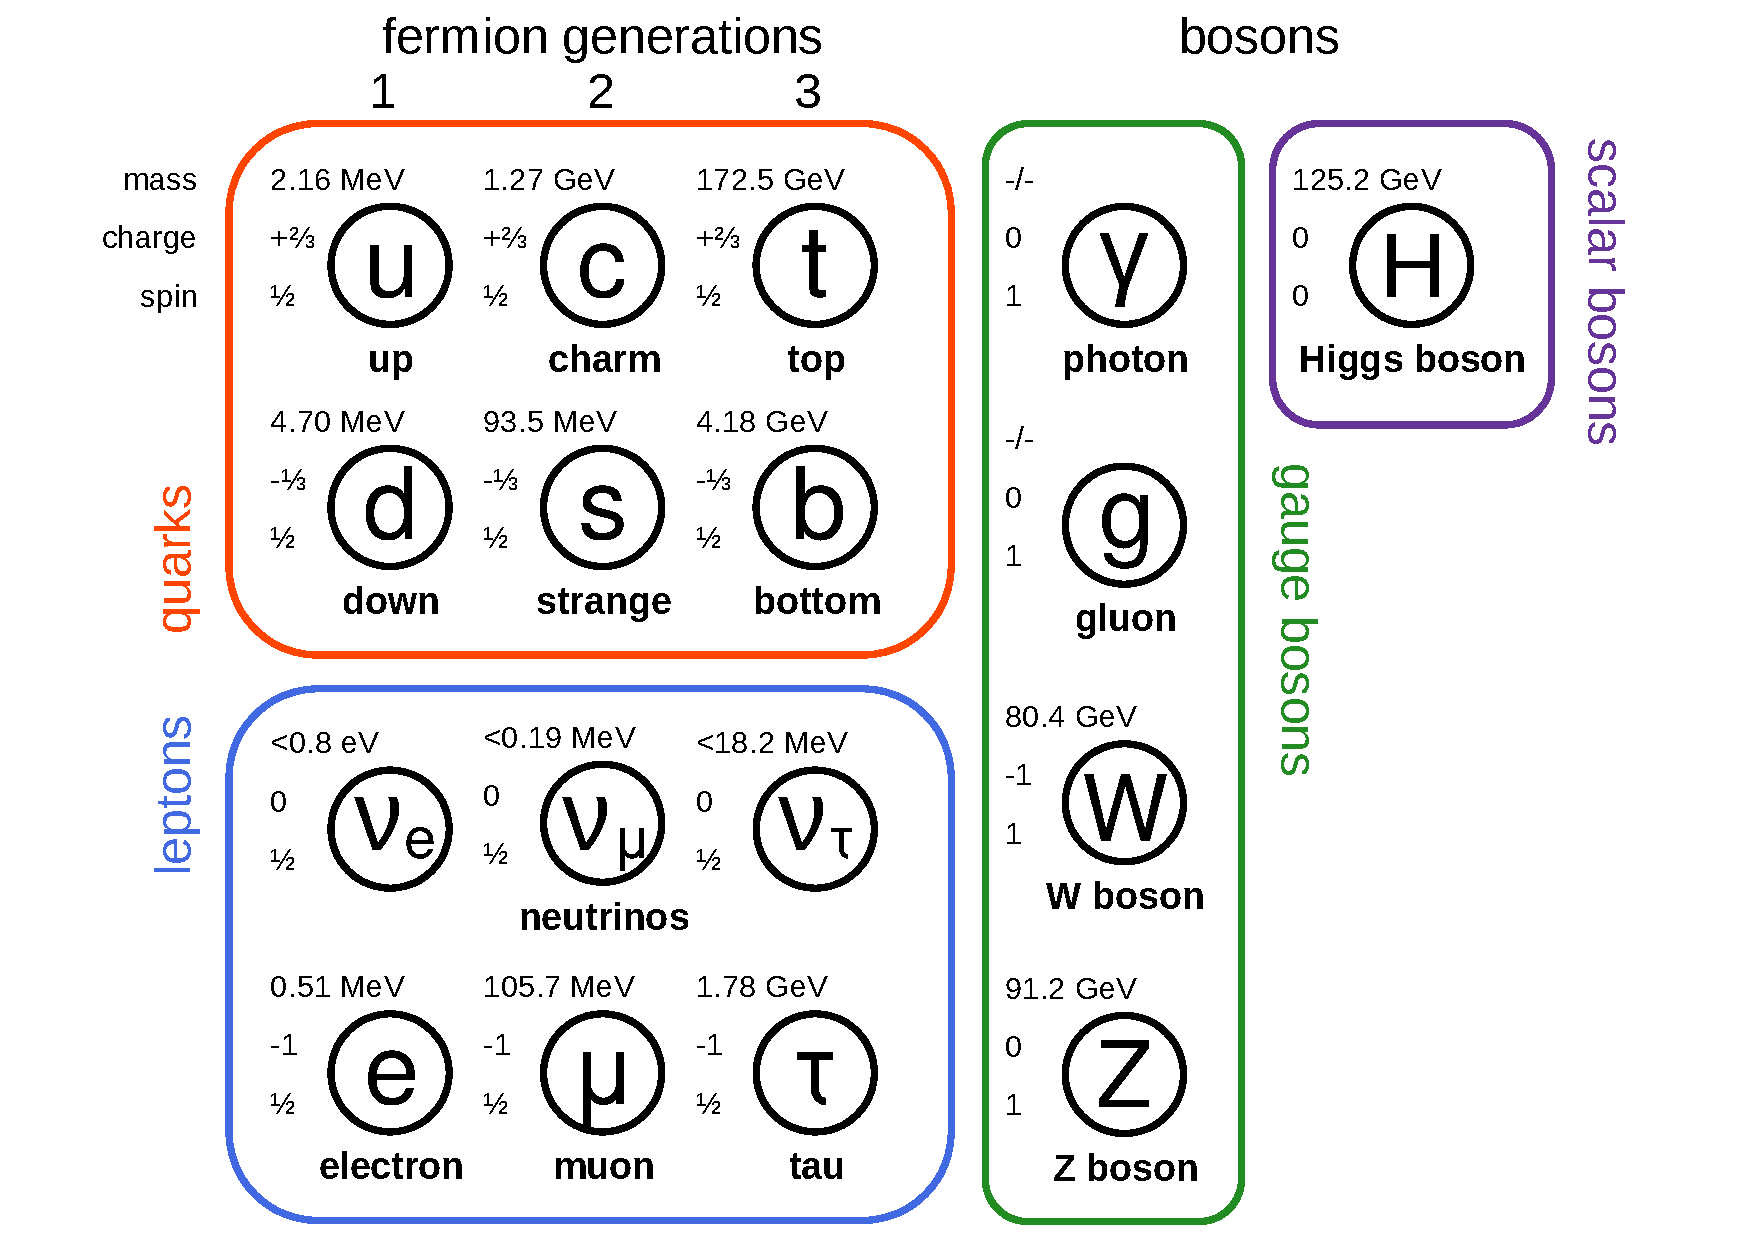
\includegraphics[width=0.9 \textwidth]{figures/smsketch_colors.pdf}
    \caption{\textbf{The Standard Model.} A schematic depiction of the particle content of the SM, showing the seventeen fundamental particles, split into six quarks, six leptons, four gauge bosons, and the Higgs boson. The mass, electromagnetic charge, and spin of the particles is given next to the labels. Mass information is taken from \citere{PDG:2022pth}.}
    \label{fig:theory:sm}
\end{figure}

The SM is formulated as a relativistic quantum field theory (QFT). That is, its most fundamental objects are fields acting on four-dimensional spacetime which, after a quantization procedure, yield physically observable particles as fundamental excitations. By the usual counting scheme, there exist seventeen different such fields, which can be classified into different groups, as schematically shown in \cref{fig:theory:sm}.

The first group consists of the twelve fermions, which have spin $\frac{1}{2}$ and make up all visible matter. They are further split into the leptons, consisting of three electrically charged leptons - electron, muon, and tau lepton - and three corresponding electrically neutral neutrinos, as well as the quarks, of which there are six different flavors, called up, down, strange, charm, bottom, and top. The quarks have fractional electric charge, and in addition carry color charge as their defining property. Of note is that the fermions are also split into three generations, with each generation consisting of a charged lepton, a neutrino, and two quarks. The only fundamental differences between the particles of different generations are their masses, though the resulting physically observable properties, such as the lifetime, might be dramatically different.

The second group of particles are the bosons, which have integer spin. Here, the four gauge bosons with spin 1 act as the force carriers of the four fundamental interactions described by the SM: the photon, for the electromagnetic interaction with coupling strength $\alpha_{\mathrm{elm}}$; the W and Z bosons, for the weak interaction with coupling strength $\alpha_W$; and the gluon, for the strong interaction with coupling strength \alphas. At high enough energies, the electromagnetic and weak interaction unify into the electroweak interaction (coupling strength \alphaew). The last and final particle is the Higgs boson, which has spin 0. Its most important role in the SM is to give mass to the fermions, as well as the W and Z bosons, through the so-called Higgs mechanism~\cite{Higgs:1964ia,Englert:1964et}, which is briefly outlined in \cref{sec:theory:higgs}.

\subsection{Quantum Chromodynamics}
\label{sec:theory:qcd}

The sector of the SM relating to the strong interaction is called \textit{quantum chromodynamics} (QCD). It is a non-Abelian gauge theory with underlying gauge group $SU(3)$, the gluon as its gauge boson and coupling strength \alphas as stated above~\cite{Schwartz:2014sze,Peskin:1995ev}. The charge under $SU(3)$ is called \textit{color charge} and is carried by all quarks, as well as by the gluon itself, which is a consequence of the non-Abelian nature of the $SU(3)$ group. Because of this, gluons can self-interact both through three-gluon and four-gluon vertices.

The self-interaction of gluons has drastic implications for the phenomenology of the theory. Because of it, the potential between to color-charged particles (i.e. quarks) rises with the distance between the two particles. This is in contrast to the electromagnetic interaction, where the Coulomb potential between two charged particles, as mediated by the photon, approaches zero for large distances. Due to this behavior, when the distance between two quarks of opposite color increases, the energy stored in the gluon field similarly increases until it is large enough to form another quark-antiquark pair from the vacuum. In this simplified picture, the two quarks from this pair would then form two bound states with the original two quarks, giving two composite particles which are color-neutral on the outside~\cite{Schwartz:2014sze}.

This principle, called \textit{confinement}, is fundamental to QCD: at low energies, no free colored particles can be observed. Because of this, quarks at low energies always form color-neutral bound states, which can be \textit{mesons} consisting of a quark and an antiquark, such as the pion, or \textit{hadrons} consisting of three quarks or three antiquarks, such as the proton and the neutron making up most visible matter. Protons and neutrons in particular consist of three light quarks (two up quarks and a down quark for the proton, and one up quark and two down quarks for the neutron) as well as a \textit{sea} of further quarks and gluons, which arise from vacuum fluctuations. The details of the proton structure, like many low-energy QCD phenomena, are nonperturbative and cannot be computed analytically from the first principles of QCD (though they can in part be inferred using heavy numerical calculations in lattice QCD). They are quantitatively described by the \textit{parton distribution functions} (PDFs), which can be seen as the probability to find a specific parton (gluon or quark) inside the proton at a given energy and momentum. More details about the description of protons in collider experiments is given in \cref{sec:mc:me}.

By contrast, at high energies, the potential between quarks reverts to the Coulomb potential, and the strong interaction slowly diminishes in strength. This behavior is called \textit{asymptotic freedom} and makes perturbative calculations for collider experiments possible. This is further reflected in the \textit{running} of the strong coupling \alphas as a function of the energy scale of the process: it slowly decreases for high energies, while it tends towards infinity at the \textit{Landau pole} located at $\Lambda_{\mathrm{QCD}} \approx \SI{250}{\MeV}$. This marks the scale at which QCD becomes nonperturbative~\cite{Peskin:1995ev,Skands:2012ts}.

\subsection{Top quark}

This thesis focuses on one particular strongly interacting fundamental particle: the top quark. As such, it will be described in further detail in this section.

The top quark was first discovered in 1995 at the Tevatron by the CDF and D0 experiments~\cite{CDF:1995wbb,D0:1995jca}. With a rest mass of $m_t \approx \SI{172.5}{\GeV}$~\cite{ATLASCMS:2024dxp}, the top quark is the most massive known fundamental particle, and as a result it has unique properties compared to the other quarks: Its extremely short lifetime of $\sim \SI{5e-25}{\s}$ is lower than the typical time needed for a quark to hadronize under the strong interaction, making it the only bare quark - that is, the only quark which,  via its decay products, is observable outside of hadrons. Among others, a consequence of this is that it fully preserves spin information during its decay, while such information is typically lost for other quarks during hadronization. More details on this are found in \cref{sec:theory:spindensity}.

A second important property of the top quark that follows from its high mass is its large Yukawa coupling to the SM Higgs boson, which is of order one. As a result, the Higgs boson couples preferentially to the top quark of all SM fermions, and the study of both the SM Higgs boson and hypothetical additional Higgs bosons (see \cref{sec:theory:bsm}) is tightly connected to the top quark. 

In the SM, the top quark decays to a bottom quark and a W boson with a branching ratio (BR) of almost 100\% (to the degree that all other decays are commonly neglected). The W boson, in turn, can decay either to a charged lepton (e, $\mu$ or $\tau$) and the corresponding neutrino with a BR of $\sim32.6\%$, or to a pair of quarks (one up- and one down-type) with a BR of $\sim67.4\%$. This results in different final states for top production processes, which are discussed more in \cref{sec:theory:ttbar}.

\subsection{Higgs mechanism}
\label{sec:theory:higgs}

The Higgs boson is the most recently discovered particle of the SM. Its existence was confirmed in 2012 at the LHC by the ATLAS and CMS collaborations~\cite{ATLAS:2012tfa,CMS:HIG-12-028,CMS:HIG-12-036}, establishing the SM in its current form as the accepted description of elementary particle physics. In the SM, the Higgs boson is described by the so-called Higgs mechanism. It is briefly discussed in this section due to its relevance for many SM extensions involving additional Higgs bosons, as searched for in \cref{ch:ah,ch:alps}.

In the SM Lagrangian, the Higgs boson appears as a complex doublet $\phi$ in the form

\begin{equation}
    \mathcal{L}_{\mathrm{SM}} \subset \left(D_\mu \phi\right)^\dagger D^\mu \phi + V(\phi)
\end{equation}

\noindent where $D_\mu$ is the covariant derivative, containing the minimal coupling to the gauge fields, and the Higgs potential $V(\phi)$ is 

\begin{equation}
    V(\phi) = \mu^2 \phi^\dagger \phi - \lambda (\phi^\dagger \phi)^2 .
\end{equation}

Here, $\mu^2$ and $\lambda$ are free parameters of the model. If both parameters are positive, this potential (known as the ``Mexican hat potential'') has a minimum at a non-zero value of

\begin{equation}
    | \phi | = \frac{\mu}{\sqrt{2 \lambda}} \equiv \frac{v}{\sqrt{2}}
\end{equation}

\noindent with the vacuum expectation value $v = \mu / \sqrt{\lambda}$. On the other hand, the minimum - corresponding to the vacuum state - is degenerate with respect to the three phases (i.e. the $SU(2)$ symmetry) of the complex doublet.

In the Higgs mechanism, this symmetry is now spontaneously broken in the transition from the high-energy state of the early universe (where the minimum is at $|\phi| = 0$) to the low-energy state observed today. The physical particles after symmetry breaking are then described by fluctuations around the new vacuum state. If the Higgs field were to be considered on its own, this would lead to one massive (corresponding to fluctuations in the $|\phi|$ direction) and three massless degrees of freedom (corresponding to the phases).

However, the interaction with the electroweak gauge fields encoded within $D_\mu$ leads to the massless degrees of freedom being absorbed into the gauge fields. This turns three of the four massless spin-1 gauge fields of the electroweak Lagrangian (with two degrees of freedom each) into massive fields instead (which have an additional longitudinal polarization, and thus three degrees of freedom). These three massive gauge fields are identified with the W and Z bosons, while the remaining massless field is identified with the photon. Finally, the leftover massive degree of freedom from the Higgs doublet $\phi$ is identified with the spin-0 boson observed at the LHC.

The resulting masses of the Z, W and Higgs bosons can be calculated as a function of $\mu^2$, $\lambda$ and the electroweak couplings and thus used to test the Higgs mechanism. In addition to the electroweak bosons, the Higgs mechanism can also give masses to fermions (charged leptons and quarks) by including a Yukawa interaction term in the Lagrangian. This results in couplings between the SM Higgs boson and the different fermions that are proportional to the respective fermion mass. 

In many possible extensions of the SM, the simple Higgs mechanism as presented here is extended or replaced by more complex theories. This can lead to modifications to the Yukawa couplings, making Yukawa coupling measurements attractive as tests of the SM. Two examples of such extensions are discussed in \cref{sec:theory:twohdm,sec:theory:alps}.

\section{The \texorpdfstring{\pptt}{pp -> tt} process}
\label{sec:theory:ttbar}

In proton-proton collisions at the LHC, the dominant production mode of top quarks is the production of a top-antitop quark pair (\ttbar). The different parts of this thesis all focus on this process in different ways, and so this chapter gives a detailed overview of relevant effects.

At LO in QCD, there are three diagrams (up to permutations of initial and final states) contributing to \ttbar production, which can be seen in \cref{fig:theory:ttbar}. They differ in their initial states: the first two diagrams are induced by gluon fusion, while the last one is induced by quark fusion (mostly from $\mathrm{u \bar{u}}$ and $\mathrm{d \bar{d}}$). The fraction of these is determined by the corresponding parton densities; at a center-of-mass energy of $\sqrt{s} \geq \SI{13}{\TeV}$, gluon fusion dominates with a fraction of roughly 90\%.

\begin{figure}[t]
    \centering
    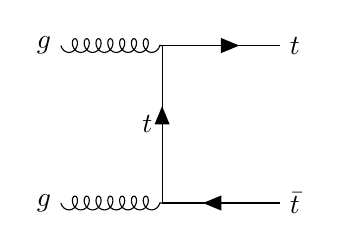
\begin{tikzpicture}[baseline=(current bounding box.center)]
      \begin{feynman}
        \vertex (i1) {\(g\)};
        \vertex [below=2.0 cm of i1] (i2) {\(g\)};
        \vertex [right=1.5 cm of i1] (a);
        \vertex [right=1.5 cm of i2] (b);
        \vertex [right=1.5 cm of a] (f1) {\(t\)};
        \vertex [right=1.5 cm of b] (f2) {\(\bar{t}\)};
        \diagram* {
          (i1) -- [gluon] (a),
          (i2) -- [gluon] (b),
          (f1) -- [anti fermion] (a) -- [anti fermion, edge label'=\(t\)] (b) -- [anti fermion] (f2)
        };
      \end{feynman}
    \end{tikzpicture}
    \hfill
    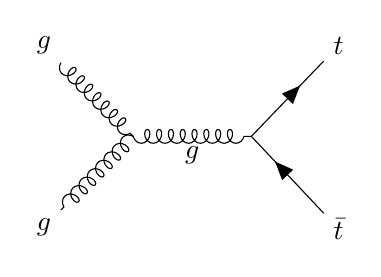
\begin{tikzpicture}[baseline=(current bounding box.center)]
      \begin{feynman}
        \vertex (a) ;
        \vertex [above left=1.3 cm of a] (i1) {\(g\)};
        \vertex [below left=1.3 cm of a] (i2) {\(g\)};
        \vertex [right=1.5 cm of a] (b);
        \vertex [above right=1.3 cm of b] (f1) {\(t\)};
        \vertex [below right=1.3 cm of b] (f2) {\(\bar{t}\)};
        \diagram* {
          (i1) -- [gluon] (a) -- [gluon] (i2),
          (a) -- [gluon, edge label'=\(g\)] (b),
          (f1) -- [anti fermion] (b) -- [anti fermion] (f2)
        };
      \end{feynman}
    \end{tikzpicture}
    \hfill
    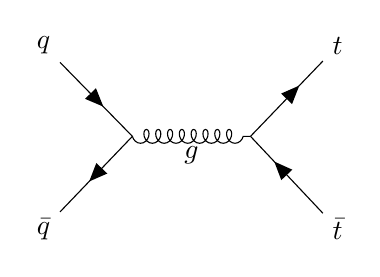
\begin{tikzpicture}[baseline=(current bounding box.center)]
      \begin{feynman}
        \vertex (a) ;
        \vertex [above left=1.3 cm of a] (i1) {\(q\)};
        \vertex [below left=1.3 cm of a] (i2) {\(\bar{q}\)};
        \vertex [right=1.5 cm of a] (b);
        \vertex [above right=1.3 cm of b] (f1) {\(t\)};
        \vertex [below right=1.3 cm of b] (f2) {\(\bar{t}\)};
        \diagram* {
          (i1) -- [fermion] (a) -- [fermion] (i2),
          (a) -- [gluon, edge label'=\(g\)] (b),
          (f1) -- [anti fermion] (b) -- [anti fermion] (f2)
        };
      \end{feynman}
    \end{tikzpicture}
    \caption{\textbf{Feynman diagrams for \pptt.} The three diagrams (up to permutations) that contribute to the \pptt process at LO in QCD.}
    \label{fig:theory:ttbar}
\end{figure}

At NLO in QCD, many more diagrams become relevant, including those induced by the fusion of one quark and one gluon, while radiating a real quark. Similarly, real emissions of gluons can take place in $gg$ or $q\bar{q}$ fusion diagrams. These effects change the kinematic properties of the produced top quarks, leading to NLO corrections for predicted distributions.

After production, both the top and antitop quark in the \ttbar pair dominantly decay into a W boson and a b (anti)quark each. This leads to three different decay channels of the \ttbar pair depending on the decays of the two W bosons, which are classified according to their number of leptons: The dilepton channel, with final state $b \bar{b} \ell^+ \ell^- \nu \bar{\nu}$; the lepton+jets channel, with final state $b \bar{b} \ell \nu q \bar{q}$; and the all-hadronic channel, with final state $b \bar{b} q q \bar{q} \bar{q}$. Here, $q$ stands in for any light quark ($u$, $d$, $s$ or $c$).

The three channels differ greatly in their experimental challenges: The dilepton channel has the lowest branching ratio of $\sim10.6\%$, which is further reduced to $\sim6.4\%$ when excluding $\tau$ leptons decaying to hadrons due to then being experimentally hard to reconstruct. It also suffers from the fact that the two produced neutrinos escape the detector unobserved and are only measured as missing transverse momentum, losing both information in the forward direction as well as the ability to disentangle the two neutrinos. On the other hand, the final state of two opposite-sign charged leptons, two b jets, and missing transverse momentum does not have many other contributing processes in the SM, leading to very pure selections (particularly when the two leptons are an electron and a muon). All results in this thesis make use of this channel prominently.

By contrast, the lepton+jets channel has a large BR of $\sim43.9\%$ ($\sim30.4\%$ when excluding $\tau$ leptons decaying to hadrons), leading to high data statistics, and allows for easier interpretation of the missing transverse momentum due to only one neutrino. However, it can suffer from contamination by W+jets and multijet QCD background (the latter with non-prompt or fake leptons), from issues with combinatorics (i.e. the assignment of experimentally measured jets to the decay products) and from hadronic jet uncertainties, which can be large. This decay channel is employed for the result in \cref{ch:ttxs} as well as in the combination in \cref{ch:ah}.

Finally, the all-hadronic channel, with a similar BR of $\sim45.4\%$, is typically difficult to isolate from the background of QCD multijet production, and in addition suffers even more strongly from combinatorics and jet uncertainties then the lepton+jets channel. As a result, it is in many cases the least precise of the three channels, and is not studied further in this work.

\subsection{Spin state of the \ttbartitle system}
\label{sec:theory:ttbarspin}

As fermions with spin $\frac{1}{2}$, top quarks have two possible spin states. As a result, the relative spins of the \ttbar system can be either aligned, leading to a total vector state with spin $S = 1$, or anti-aligned, leading to a scalar state with spin $S = 0$. Furthermore, the \ttbar system as a whole can have orbital angular momentum $L$, where $L$ is a non-negative integer. 

In analogy to atomic orbitals, the total angular momentum is then $\vec{J} = \vec{L}+\vec{S}$, and for any chosen basis the set of quantum numbers $\{S,L,J,J_z\}$ consists of conserved quantities. The angular momentum state is commonly written using a term symbol ${}^{2S+1}L_{J}$, where $2S+1$ denotes the multiplicity of the spin state, and the orbital angular momentum $L$ is written using spectroscopic notation (S for $L=0$, P for $L=1$, D for $L=2$ etc). An overview of the lowest possible states ($J \leq 1$) is given in \cref{tab:theory:spinstates}, including also the parities and charge-parities $\mathcal{P}$ and $\mathcal{C}$, which can be inferred from the intrinsic parities of top and antitop as well as the orbital angular momentum. In proton-proton collisions, a mixture of all these states is produced, with the ratio depending on the production mode ($gg$, $q\bar{q}$ or $gq$), the energy, and the kinematics of the collision. Measurements of the spin and angular momentum state of the \ttbar systems produced at the LHC thus give information about the details of the production mechanism, and can be attractive tests of the SM.

\begin{table}[]
    \centering
    \begin{tabular}{c|c|c|c|c}
         Term symbol & Spin multiplicity & $\mathcal{P}$ & $\mathcal{C}$ & \CP \\
         \hline
         \hline
         \term{1}{S}{0} & singlet & $-1$ & $+1$ & $-1$ \\
         \term{3}{P}{0} & triplet & $+1$ & $+1$ & $+1$ \\
         \term{3}{S}{1} & triplet & $-1$ & $-1$ & $+1$ \\
         \term{1}{P}{1} & singlet & $+1$ & $-1$ & $-1$ \\
         \term{3}{P}{1} & triplet & $+1$ & $+1$ & $+1$ \\
         \term{3}{D}{1} & triplet & $-1$ & $-1$ & $+1$
    \end{tabular}
    \caption{\textbf{Spin states of \ttbar.} Overview of the possible angular momentum states of the \ttbar system with $J \leq 1$, including the spin multiplicity, the parity $\mathcal{P}$, the charge-parity $\mathcal{C}$, and their product \CP.}
    \label{tab:theory:spinstates}
\end{table}


\begin{figure}[t]
    \centering
    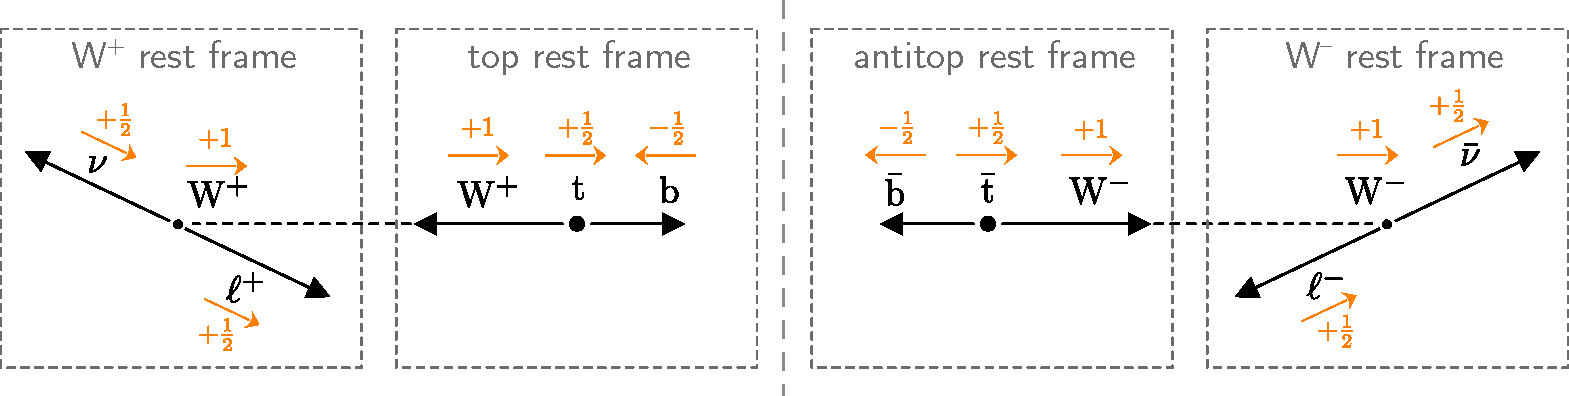
\includegraphics[width=\linewidth]{figures/spin_corrs_sketch_v3.pdf}
    \caption{\textbf{Helicity in top decays}. Sketch of the allowed helicity configurations in a top (left) and antitop quark decay (right) to a lepton. The orange arrows and numbers illustrate the spin of the respective particles. The (anti)top decay is shown in the (anti)top rest frame, and the W boson decay in the W boson rest frame, as indicated by the gray boxes. It can be seen that, due to conservation of angular momentum and the parity-violating nature of the weak interaction, the $\ell^+$ is preferred to be emitted in the direction of the $t$ spin, while the $\ell^-$ is preferred to be emitted opposite to the direction of the $\bar{t}$ spin.}
    \label{fig:theory:topspin}
\end{figure}

In practice, the spins of the top (anti)quarks cannot be observed directly, and instead must be inferred from their decay products. The way in which the spin information is passed to the decay products is determined by the maximally parity-violating nature of the weak interaction as well as by conservation of angular momentum. This is illustrated in \cref{fig:theory:topspin} (left) for the leptonic decay of the top (anti)quark: Since the b quark is almost massless compared to the top quark, so that $m_{\mathrm{b}} = 0$ can be assumed in the following, it will be ultra-relativistic. Like for all fermions, its helicity is thus determined by its chirality. As a result, for the decay $t \rightarrow W^+ b$ the b quark - left-handed due to the weak interaction - has negative helicity (spin opposite to its direction of flight), leading to a longitudinally polarized W boson through conservation of angular momentum.

Since the decay of the $W^+$ into $\ell^+ \nu$ is again mediated by the weak interaction, and both decay products are nearly massless, the helicities of $\ell^+$ and $\nu$ must be positive and negative, respectively. Boosting into the $W^+$ rest frame (leftmost box in \cref{fig:theory:topspin}), and again applying conservation of angular momentum, one then finds from the sketch that the charged lepton is emitted preferably in the direction of the top quark spin. 

Repeating the same line of arguments for the decay of the antitop (\cref{fig:theory:topspin} right), one finds that the opposite holds there: the charged lepton is emitted preferably opposite to the antitop spin. As a result, the direction of flight of the charged lepton in the center-of-mass system of its parent (anti)top can be used as a proxy for the (anti)top spin (or, equivalently, its polarization). It should be noted that this property of the top quark is unique among the quarks of the SM, since all other quarks hadronize via the helicity-ignorant strong interaction and thus lose the largest part of their spin information\footnote{See e.g. \citere{Kats:2023zxb} for the greatly reduced possibilities of measuring spin correlations in \bbbar or \ccbar systems at the LHC.}.

Returning to the full \ttbar system, and applying the above observation to both top and antitop, one can now define observables to probe the \ttbar spin state, or equivalently, the spin correlation between $t$ and $\bar{t}$. A simple such variable is the azimuthal difference \dphill between the two leptons in a dileptonic decay. Assuming that the top and antitop are emitted back-to-back, a state with the top and antitop spins aligned (i.e. $S=1$) will cause the two leptons to be emitted preferably in opposite directions, leading to large \dphill, while anti-aligned spins ($S=0$) will lead preferably to parallel leptons and thus small \dphill. While this variable has the advantage of being easy to define and experimentally clean to measure, it is suboptimal in that it is also strongly affected by the kinematics of the \ttbar production, including higher-order corrections in QCD, and is heavily sculpted when selecting certain areas of \ttbar phase space. Thus, it is afflicted with large modeling uncertainties.

A more powerful variable can be defined by employing suitable reference systems as follows: the lepton and antilepton are first Lorentz boosted into the center-of-mass frame of the \ttbar system, and then further boosted into the center-of-mass frame of their parent (anti)tops. Then, a correlation variable \chel is defined as the scalar product of their direction unit vectors in these reference frames\footnote{
In this work, the naming convention from \citere{CMS:HIG-17-027} is followed for \chel. In e.g. \citere{Bernreuther:2004jv}, this variable is instead called $\cos \varphi$.
}:

\begin{equation}
\label{eq:theory:cheldef}
    \chel = \hat{\ell}^+_{t} \cdot \hat{\ell}^-_{\bar{t}} 
\end{equation}

It can be shown that, irrespective of the mode of production of the \ttbar system and inclusive in the rest of the phase space, the distribution of this observable always follows a straight line~\cite{Bernreuther:2004jv}, i.e.

\begin{equation}
\label{eq:theory:chel}
    \frac{1}{\sigma} \frac{d \sigma}{d \chel} = \frac{1}{2} \left( 1 - D \, \chel \right)
\end{equation}

The slope $D$ depends on the spin and angular momentum of the produced \ttbar state. At LO in QCD, it can be shown that $D=-1$ for pure singlet states (anti-aligned spins, e.g. \term{1}{S}{0}, \term{1}{P}{1}) and $D=+\frac{1}{3}$ for pure triplet states (aligned spins, e.g. \term{3}{S}{1}, \term{3}{P}{0})~\cite{Maltoni:2024tul,Cheng:2024btk}. Higher-order corrections in QCD can slightly reduce these slopes through emissions of real gluons in the decay, which weaken the correlations, but these effects are of the order of $0.2\%$ at NLO for leptons~\cite{Czarnecki:1990pe,Bernreuther:2003ga}. %For states with orbital angular momentum, there is an additional degree of freedom in the decay since only the total angular momentum with respect to any axis is conserved. As a result, the slopes $D$ for these states are less steep; for example, the \term{3}{P}{0} state (with aligned spins) has a mildly negative slope of \todo{}.

In practice, any observed ensemble of \ttbar pairs will be a mixture of the different spin states depending on the production mechanism and underlying theory, which can be probed by measuring the slope $D$. As will be discussed in \cref{sec:theory:bsm}, extensions of the SM can change the predicted slope, making measurements of $D$ attractive tests for new physics. The value of $D$ has been measured e.g. in \citeres{CMS:TOP-14-023,CMS:TOP-18-006,CMS:TOP-23-007}, as well as more recently as a proxy variable in the context of measurements of quantum entanglement in \ttbar production~\cite{CMS:TOP-23-001,ATLAS:2023fsd}.

%$\todo{measurements of D, entanglement}

\subsection{Spin density matrix}
\label{sec:theory:spindensity}

A more detailed way to quantify the spin properties of the \ttbar system, respective to an arbitrary spin basis, is the production spin density matrix $\mathbf{R}$, which (when averaged over initial polarizations and colors, and summed over final colors but not over final polarizations) can be written as~\cite{Maltoni:2024tul,Cheng:2024btk,Anuar:PhD}

\begin{equation}
    \mathbf{R} = A \, \mathbb{1} \otimes \mathbb{1}
    + B_i^1 \, \sigma_i \otimes \mathbb{1}
    + B_i^2 \, \mathbb{1} \otimes \sigma_i
    + C_{ij} \, \sigma_i \otimes \sigma_j.
\end{equation}

Here, $\mathbb{1}$ is the two-dimensional identity matrix, $\sigma_i$ with $i=1,2,3$ are the Pauli matrices, and the first and second components of the tensor product refer to the spin of the top and antitop quark, respectively. The scalar coefficient $A$ describes the overall amplitude (i.e. the differential cross section as a function of the top and antitop kinematics) of \ttbar production, the vectors $\vec{B}^1$ and $\vec{B}^2$ describe the polarization of the top and antitop quark, and the matrix $\mathbf{C}$ describes the correlation between their spins. All of them are, in general, functions of the partonic center-of-mass energy and the scattering angle of the top quark relative to the incoming partons.

As explained in \cref{sec:theory:ttbarspin}, in a dileptonic decay the spin information is transferred almost completely to the charged leptons. Defining the lepton directions of flight in their parent (anti)top rest frames $\hat{\ell}_t^+$ and $\hat{\ell}_{\bar{t}}^-$ as in \cref{eq:theory:cheldef}, the resulting differential cross section in terms of the lepton angles, collectively denoted as $\Omega$, is~\cite{Anuar:PhD}

\begin{equation}
    \frac{1}{\sigma} \frac{d \sigma}{d \Omega} = 1 + \vec{B}^1 \cdot \hat{\ell}_t^+ + \vec{B}^2 \cdot \hat{\ell}_{\bar{t}}^- + (\hat{\ell}_t^+)^T \, \mathbf{C} \, \hat{\ell}_{\bar{t}}^- .
\end{equation}

By integrating out the remaining angles, it can be shown from this that irrespective of the chosen basis the slope $D$ as defined in \cref{eq:theory:chel} can be recovered from the matrix $\mathbf{C}$ as~\cite{Bernreuther:2004jv,Bernreuther:2017yhg}

\begin{equation}
    D = \frac{1}{3} \mathrm{Tr} \left[ \mathbf{C} \right] .
\end{equation}

\begin{figure}[t]
  \centering
  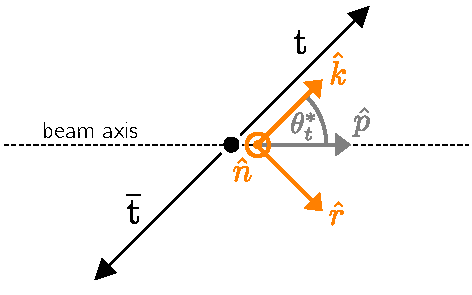
\includegraphics[width=0.6\linewidth]{figures/helicity_basis_new.pdf}
  \caption{\textbf{Helicity basis.} Sketch of the helicity basis used to define the top and antitop quark spins. The unit vectors $\hat{k}$, $\hat{r}$ and $\hat{n}$ define the right-handed basis, while the beam axis is given by $\hat{p}$ and the top quark scattering angle by $\theta^*_t$.}
  \label{fig:theory:helicitybasis}
\end{figure}

As discussed in \cref{sec:theory:ttbarspin}, $D$ is maximally negative for pure singlet states (corresponding to a positive slope in \chel). It  is thus ideal for separating those in a mixed ensemble like the one provided by \pptt production, which contains all possible spin states (cf. \cref{tab:theory:spinstates}).

One can define similar separating observables for other states using the spin density matrix by choosing a suitable spin basis. In this work, the so-called helicity basis proposed in \citere{Bernreuther:2015yna} is used. The three axes of this basis, denoted $\hat{k}$, $\hat{r}$ and $\hat{n}$, are defined as follows: $\hat{k}$ is simply the direction of flight of the top quark in the center-of-mass frame of the \ttbar system, such that the top quark spin with respect to $\hat{k}$ is equal to the helicity. The second axis, $\hat{r}$, is orthogonal to $\hat{k}$ in the scattering plane of the \pptt process. Finally, the third axis $\hat{n}$ is orthogonal on both $\hat{k}$ and $\hat{r}$, oriented such that the $\{\hat{k},\hat{r},\hat{n}\}$ system is left-handed. If $\hat{p}$ denotes the beam axis and $\theta^*_t$ the top scattering angle with respect to this axis, the latter two axes are given by

\begin{equation}
    \hat{r} = \frac{\hat{p} - \cos \theta^*_t \hat{k}} {| \hat{p} - \cos \theta^*_t \hat{k} |} \quad \mathrm{and} \quad \hat{n} = \hat{r} \times \hat{k} = \frac{\hat{p} \times \hat{k}} {| \hat{p} \times \hat{k} |}.
\end{equation}

This coordinate system is visualized in \cref{fig:theory:helicitybasis}. It is used, among others, in \citeres{CMS:TOP-18-006,CMS:TOP-23-007} to measure both the polarizations $\vec{B}^1$ and $\vec{B}^2$ and spin correlation coefficients $C_{ij}$ ($i,j = k,r,n$). In this work, only the spin correlation is considered. Particularly, in addition to \chel, the following observable is defined:

\begin{equation}
    \label{eq:theory:chan}
    \chan = - (\hat{\ell}_t^+)_k (\hat{\ell}_{\bar{t}}^-)_k + (\hat{\ell}_t^+)_r (\hat{\ell}_{\bar{t}}^-)_r + (\hat{\ell}_t^+)_n (\hat{\ell}_{\bar{t}}^-)_n
\end{equation}

\noindent where $(\hat{\ell})_i$, $i=k,r,n$ refers to the $i$-th component of the respective vector in the $\{k,r,n\}$ basis. For comparison, using the same notation, \chel can be written as

\begin{equation}
    \label{eq:theory:chel_components}
    \chel = + (\hat{\ell}_t^+)_k (\hat{\ell}_{\bar{t}}^-)_k + (\hat{\ell}_t^+)_r (\hat{\ell}_{\bar{t}}^-)_r + (\hat{\ell}_t^+)_n (\hat{\ell}_{\bar{t}}^-)_n .
\end{equation}

The only difference between \chel and \chan thus lies in the sign of the first term encoding the correlation in the $\hat{k}$ direction, i.e. the top direction of flight.
Like \chel, \chan has the advantage of always being linear in the absence of phase space cuts, i.e.

\begin{equation}
    \frac{1}{\sigma} \frac{d \sigma}{d \chan} = \frac{1}{2}\left( 1 + D^{(k)} \chan \right)
\end{equation}

\noindent where~\cite{Maltoni:2024tul}

\begin{equation}
\label{eq:theory:Dk}
    D^{(k)} = \frac{1}{3} \left( C_{kk} - C_{rr} - C_{nn} \right) .
\end{equation}

From \cref{eq:theory:Dk}, it can be seen that the slope is maximally negative, $D^{(k)} = -1$, when the top and antitop spins are anti-correlated along the top direction of flight ($C_{kk} = -1$) and correlated along the orthogonal directions ($C_{rr} = C_{nn} = +1$). The (unpolarized) state described by these correlations is a pure triplet state ($S=1$)~\cite{Maltoni:2024tul}. 

Particularly, the \term{3}{P}{0} state of \ttbar always corresponds to this spin state: It has no total angular momentum, so that its total spin and orbital angular momentum must be anti-aligned. Since the orbital angular momentum is always exactly zero in the direction of flight of the top quarks, the \ttbar system must be in an orbital angular momentum eigenstate with $L_k = 0$, and thus also in a total spin eigenstate with $S_k = 0$. In other words, the spins in the $\hat{k}$ direction are anti-aligned, corresponding to $C_{kk} = -1$. In order to arrive at $S=1$, i.e. a pure triplet state, it is required that the other entries fulfill $C_{rr} = C_{nn} = 1$.


% next: a) choice of basis - helicity basis by Bernreuther
% b) decay products - weak interaction (V-A), ??? try to understand this shit

\section{Bound state effects in \ttbartitle}
\label{sec:theory:etat}

When predicting distributions of observables for hard scattering processes such as \ttbar production, one usually employs perturbative calculations at a fixed order in the strong coupling constant \alphas, possibly matched to a parton shower (see \cref{ch:mc}). However, at low energy scales (or equivalently, long distances) the strong interaction becomes nonperturbative, leading to effects that cannot be captured in the usual perturbative expansion irrespective of the order in \alphas (though they might or might not be captured in expansions or resummations with other parameter choices).

For other quarks, long-distance effects are well known to lead to the formation of quark-antiquark bound states, called \textit{quarkonia}. Examples for \ccbar and \bbbar production are $\mathrm{J/\psi}$, $\eta_c$ or $\Upsilon$. An important question is now whether a similar bound state (``toponium'') exists for \ttbar production, which will be discussed in detail in this section.

\subsection{Properties of a \ttbartitle bound state}
\label{sec:theory:toponium_properties}

To begin, some simple properties of a possible toponium are roughly estimated by adapting the simple picture of a non-relativistic bound state. The top quark and antiquark are, for now, seen as stable particles bound by QCD, in analogy how proton and electron are bound by the electric force inside the hydrogen atom. The QCD potential between quark and antiquark as a function of the radius $r$ can be approximated as\footnote{In general, the potential also contains a linear term proportional to $r$ parameterizing the self-interaction of gluons in QCD and the resulting confinement~\cite{Deur:2016tte}. However, it is small for systems of sufficiently small size like toponium and thus neglected for the simple estimation in this section.}

\begin{equation}
  V_{\mathrm{QCD}}^{[1,8]} (r) = - \frac{C^{[1,8]} \alphas}{r} + \order{\alphas^2} ,
\end{equation}

\noindent where the color factor is $C^{[1]} = 4/3$ for color-singlet and $C^{[8]} = -1/6$ for color-octet \ttbar states. As a result, only \ttbar systems in a color-singlet state feel an attractive force and can possibly form a bound state, while color-octet states are instead repulsed.

In analogy with the hydrogen atom, one can now estimate the binding energy of a color-singlet \ttbar bound state as~\cite{Fadin:1987,Fabiano:1994cz,Maltoni:LHCTopWG}

\begin{equation}
\label{eq:theory:toponium_eb}
  E_b = -\frac{1}{2} \frac{\mt}{2} \left( C^{[1]} \alphas \right)^2
\end{equation}

\noindent and the Bohr radius of the bound state as

\begin{equation}
\label{eq:theory:toponium_rb}
  r_b = \frac{2} {C^{[1]} \alphas \mt} .
\end{equation}

To evaluate this numerically, the scale at which \alphas should be evaluated needs to be defined. An intuitive choice is the inverse of the Bohr radius $1/r_b$, corresponding to the typical energy scale of the (anti)quark~\cite{Kiyo:2008bv,Maltoni:LHCTopWG}. At one loop in QCD, the running of \alphas is given by~\cite{Schwartz:2014sze}

\begin{equation}
  \alphas (Q^2) = \frac{\alphas(m_Z^2)}{ 1 + \beta_0 \, \alphas(m_Z^2) \ln \left( \frac{Q^2}{m_Z^2} \right)} \quad \text{with} \quad \beta_0 = \frac{33 - 2 N_f}{12 \pi}
\end{equation}

\noindent where $N_f = 5$ is the number of active quark flavors and $\alphas(m_Z^2) = 0.118$ is the strong coupling constant at the reference scale of the Z boson mass, $m_Z = \SI{91.2}{\GeV}$~\cite{PDG:2022pth}.
Replacing \alphas by $\alphas(1/r_b)$ in \cref{eq:theory:toponium_rb} yields a self-consistent equation with the numerical solution

\begin{equation}
\label{eq:theory:alphas_toponium}
  \alphas(1/r_b) = 0.158 \quad \text{and} \quad r_b = \SI{0.056}{\per\GeV} \approx \SI{0.01}{\femto\meter} .
\end{equation}

This extremely small radius would make a possible \ttbar bound state the smallest known non-pointlike object~\cite{Fu:2025yft}.

Inserting $\alphas(1/r_b)$ into \cref{eq:theory:toponium_eb} finally gives for the binding energy and ``mass'' of toponium:

\begin{equation}
\label{eq:theory:toponium_eb_num}
  E_b = - \SI{1.93}{\GeV} \quad \implies \quad M = 2 \mt + E_b \approx \SI{343}{\GeV}
\end{equation}

\noindent where a value of $\mt = \SI{172.5}{\GeV}$ was used for the top quark mass. Varying the scale used to evaluate \alphas up and down by a factor 2, as typically done, results in a variation of $\Delta E_b \approx \pm\SI{0.5}{\GeV}$. A further useful quantity is the average velocity of the top (anti)quarks in the bound state, given simply by (in units of the speed of light)~\cite{Maltoni:LHCTopWG}:

\begin{equation}
  v_0 = C^{[1]} \alphas = 0.21 .
\end{equation}

However, this simple picture is spoiled by the large width of the top quark of about $\Gammat = \SI{1.4}{\GeV}$~\cite{PDG:2022pth} and resulting short average lifetime of $\tau_\mathrm{t} \approx 5 \times 10^{-25}$~s. Since both the top quark and antiquark making up the bound state can in principle decay independently, the dominant decay of toponium will be through disassociation, i.e. through one of the constituent quarks decaying to $Wb$ as usual~\cite{Fabiano:1994cz}. The width and lifetime of toponium can thus be respectively estimated as $2 \Gammat$ and $\frac{1}{2} \tau_\mathrm{t}$. This can be compared to the formation time of toponium, estimated as the classical revolution time of the quark and antiquark and given by~\cite{Maltoni:LHCTopWG}

\begin{equation}
  \tau_{\mathrm{form}} = \frac{2 \pi r_b}{v_0} \approx 1 \times 10^{-24}~\si{\second} .
\end{equation}

Since $\tau_{\mathrm{form}} > \frac{1}{2} \tau_\mathrm{t}$, either the top or the antitop quark will in most cases decay before toponium can form, so that \ttbar does not form stable bound states~\cite{Fabiano:1994cz,Fadin:1987}. One can estimate the fraction of at-rest \ttbar pairs that live long enough to form a bound state by approximating the lifetime of a \ttbar system through an exponential distribution, which gives $\exp(-2 \tau_{\mathrm{form}} / \tau_\mathrm{t}) \approx 1\%$. Based on this simple picture, \ttbar bound state formation is expected to be a rather small effect.

\subsection{Non-relativistic QCD calculations}

A more quantitative picture of \ttbar bound state effects is given by the framework of non-relativistic QCD (NRQCD)~\cite{Fadin:1990wx,Sumino:2010bv,Kiyo:2008bv,Garzelli:2024uhe}. 
In this approach, the partonic differential cross section for the production of a \ttbar pair from two initial state partons $i$ and $j$ as a function of its invariant mass \mtt can be written in a factorized form as~\cite{Kiyo:2008bv}

\begin{equation}
\label{eq:theory:ttbar_factorization}
  \frac{d \hat{\sigma}(ij \rightarrow \ttbar)}{d \mtt} (\hat{s}, \mtt) = F_{ij \rightarrow \ttbar} (\hat{s}, \mtt) \, \frac{1}{\mt^2} \, J (\mtt)
\end{equation}

\noindent where $\hat{s}$ is the partonic center-of-mass energy squared\footnote{At LO in QCD, there is no additional radiation, and so $\hat{s} = \mtt^2$.}, $F_{ij \rightarrow \ttbar} (\hat{s}, \mtt)$ is the \textit{hard function}, which contains the hard scattering matrix element for \pptt, and $J (\mtt)$ is the \textit{long-distance function} that encodes possible bound state effects. The hard function can be computed in the usual manner in relativistic perturbative QCD at a fixed order in \alphas (cf. \cref{sec:mc:me}). The long-distance function is obtained from the solutions to the Schr\"odinger equation describing top quark and antiquark, analogously to the hydrogen atom as discussed in the previous section. Here, it is assumed that the relative velocity of the top and antitop quark is small and they can thus be considered non-relativistic.

If the top quarks are considered stable, i.e. $\Gammat = 0$, there is a discrete set of solutions with masses $M_n = 2 \mt + E_n$, and the long-distance function below the threshold is given by~\cite{Kiyo:2008bv}

\begin{equation}
\label{eq:theory:longdistance_stable}
  J(\mtt) = \sum_n | \Psi_n (0) |^2 \pi \delta(\mtt - M_n)
\end{equation}

\noindent where $| \Psi_n (0) |^2$ is the squared wave function at the origin for solution $n$. This picture thus corresponds to a discrete set of cleanly separated, stable bound states described by $\delta$ functions, similar to \ccbar and \bbbar bound states.

In practice, the finite top width is of a similar order of magnitude as the binding energy (see previous section), and cannot be neglected. One can take the finite top width into account by replacing the long-distance function with~\cite{Kiyo:2008bv}

\begin{equation}
\label{eq:theory:longdistance_unstable}
  J (\mtt) = \mathrm{Im} \, G (\vec{r} = 0; \mtt + i \Gammat)
\end{equation}

\noindent where $G (\vec{r} = 0; \mtt + i \Gammat)$ is the \textit{Green's function} of the non-relativistic Schr\"odinger equation, evaluated at zero distance ($\vec{r} = 0$) using a complex mass $\mtt + i \Gammat$. 

The long-distance function is shown numerically in \cref{fig:theory:greensfunction} for both the stable top and finite width case, evaluated at LO in QCD using the expressions in \citere{Kiyo:2008bv}. The same scales and values of \alphas as in \cref{eq:theory:alphas_toponium} have been used for the evaluation.
As discussed in the previous section, bound-state effects are only present for a color-singlet state, while for a color-octet state, the long-distance function is smaller than the long-distance function for free quarks, indicating a suppression of the cross section for color-octet states close to the threshold.

For color-singlet states, in the finite width case the bound state energy levels are no longer cleanly separated, but smeared together with the \ttbar continuum by the finite top width. The bound state and the \ttbar continuum are thus in principle not separable, and bound state effects should be seen as a correction to the usual fixed-order \ttbar continuum spectrum. Because of this, this effect is sometimes called a ``quasi-bound state'' or a ``virtual bound state".

\begin{figure}[t]
    \centering
    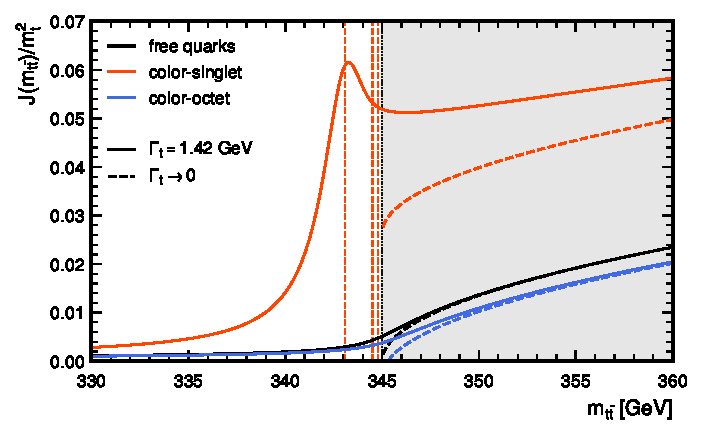
\includegraphics[width=0.85\linewidth]{figures/greensfunction.pdf}
    \caption{\textbf{Long-distance function encoding \ttbar bound state effects.} The long distance function $J(\mtt)$ (\cref{eq:theory:ttbar_factorization}), normalized to the top mass squared, as a function of \mtt around the \ttbar threshold. The free quark case (i.e. no interaction) is shown in black, and the color-singlet and color-octet cases are shown in orange and blue, respectively. Dashed lines correspond to stable top quarks ($\Gammat \rightarrow 0$, \cref{eq:theory:longdistance_stable}), split into a discrete spectrum below and a continuous spectrum above the \ttbar threshold (gray shaded area). Solid lines to the case of a finite top mass (\cref{eq:theory:longdistance_unstable}). All curves have been computed using the expressions in \citere{Kiyo:2008bv}.}
    \label{fig:theory:greensfunction}
\end{figure}

Still, a peak in the long-distance function is clearly visible at $\mtt \approx 2 \mt - \SI{2}{\GeV}$, coinciding with the binding energy estimated in the simple picture of the previous section. This location of the peak is confirmed by multiple independent full NRQCD calculations, taking into account also the hard function as well as higher orders of \alphas in the QCD potential~\cite{Fadin:1990wx,Kiyo:2008bv,Sumino:2010bv,Ju:2020otc,Garzelli:2024uhe}. The details of the line shape differ between some of the calculations, and should thus be considered uncertain. However, the experimental resolution of \mtt is expected to be much larger than the bound state width of order $\sim 2 \Gammat$ (see \cref{sec:ah:kinreco}), making the details of the spectrum irrelevant to an experimental search.

Besides the \mtt spectrum, one can infer the angular momentum state of the \ttbar bound state from the available production mechanisms at the LHC. Since \qqbar systems are always color octets, \ttbar bound states can thus at LO be produced only from gg initial states in proton-proton collisions. Since both of the top quarks have low velocity, states with orbital angular momentum $L \neq 0$ will be strongly suppressed (beyond NLO in NRQCD~\cite{Kiyo:2008bv}). Furthermore, the gg initial state in \ttbar production close to the \ttbar threshold always has spin $S = 0$ (and thus total angular momentum $J = 0$), with $S = 2$ contributions suppressed by powers of the top velocity~\cite{Cheng:2024btk}, so that the resulting \ttbar system must be in the \termc{1}{S}{0}{1} state. At NLO in QCD, also \termc{3}{S}{1}{1} states can be produced; however, the contribution is very small (less than $0.1\%$ of the total cross section~\cite{Kiyo:2008bv}).

%In the \pptt process, such effects might play a role in the vicinity of the \ttbar production threshold, i.e. for $\mtt \sim 2 \mt$, where the relative velocities of the produced top quarks become small. In particular, one possible class of effects not included in simple expansions in \alphas are \ttbar bound states (``toponium''). Such states (also called quarkonia) are well-known in \ccbar and \bbbar production, where they lead to composite particles such as $\mathrm{J/\psi}$, $\eta_c$ or $\Upsilon$. When translating this knowledge to \ttbar, however, there is a significant difference: due to the large top quark mass, the lifetime of the top quark is expected to be shorter than the (formal) lifetime of any possible \ttbar bound state. As a result, the state would in the majority of cases not decay e.g. to photons, gluons or hadrons like the lighter quarkonia, but instead disassociate by one of the constituent top quarks decaying normally to Wb. This phenomenon, sometimes called a ``quasi-bound state'' or a ``virtual bound state", would lead to a possible peak in the \mWWbb spectrum slightly below the \ttbar threshold.

% Calculations of the \mWWbb spectrum at the \ttbar threshold including the effects from a possible bound state have been performed independently in \citeres{Fadin:1990wx,Kiyo:2008bv,Sumino:2010bv,Ju:2020otc,Garzelli:2024uhe}. All of these calculations work in the framework of non-relativistic QCD (NRQCD), which treats the slowly moving ($v \ll c$) top (anti)quarks as non-relativistic particles. This approach can be seen as a low-energy effective field theory (EFT) of the SM where high-energy modes have been integrated out, or alternatively, as an alternate perturbative expansion in the ratio $\alphas/\beta$, where $\beta$ is the top quark velocity. The result is a non-relativistic Schr\"odinger equation for the wavefunction of the \ttbar system, with the interaction between the top quarks described by the low-energy limit of the QCD Coulomb potential, representing the exchange of soft gluons. At LO, it is given by~\cite{Kiyo:2008bv}

% \begin{equation}
%     V_{\mathrm{QCD}}^{[1,8]} (q) = - \frac{4 \pi \alphas C^{[1,8]}}{q^2} ,
% \end{equation}

% \noindent where the color factor is $C^{[1]} = 4/3$ for color-singlet and $C^{[8]} = -1/6$ for color-octet states. As a result, only \ttbar systems in a color-singlet state feel an attractive force and can possibly form a bound state, while color-octet states are instead repulsed. At the LHC, \ttbar bound states can thus at LO be produced only from gg initial states, since \qqbar systems are always color-octets. From this, the spin state of the produced bound state can be inferred: Since both of the top quarks have low velocity, states with orbital angular momentum $L \neq 0$ will be strongly suppressed (beyond NLO in NRQCD~\cite{Kiyo:2008bv}). Furthermore, the gg initial state in \ttbar production close to the \ttbar threshold always has spin $S = 0$ (and thus total angular momentum $J = 0$), with $S = 2$ contributions suppressed by powers of the top velocity~\cite{Cheng:2024btk}, so that the resulting \ttbar system must be in the \termc{1}{S}{0}{1} state. At NLO in QCD, also \termc{3}{S}{1}{1} states can be produced; however, the contribution is very small (less than $0.1\%$ of the total cross section~\cite{Kiyo:2008bv}).

% \citeres{Kiyo:2008bv,Sumino:2010bv,Ju:2020otc,Garzelli:2024uhe} agree that the binding energy of the \ttbar bound state, defined as the difference of the peak position in the \mWWbb spectrum to $2 \mt$, is around \SI{-2}{\GeV}, resulting in a ``mass'' of \SI{343}{\GeV} for the \ttbar bound state for a top mass of \SI{172.5}{\GeV}. The exact line shape of the peak is less well known. However, the experimental resolution of \mWWbb is expected to be much larger than the bound state width of order $\sim 2 \Gammat$ (see \cref{sec:ah:kinreco}), making the details of the spectrum irrelevant to an experimental search.

\subsection{Modeling in Monte Carlo simulation}

The existing NRQCD calculations predict only certain differential distributions and cannot be directly compared to experimental data on a per-event level. Because of this, a simplified model for the \ttbar bound state that can be used in MC simulation (cf. \cref{ch:mc}) is introduced following \citeres{Maltoni:2024tul,Maltoni:2024csn,Fuks:2021xje,Aguilar-Saavedra:2024mnm}. Instead of a first-principles calculation, the bound state effects are modeled as an additional spin-0 state \etat, which is added to the conventional perturbative QCD (pQCD) calculation of \ttbar. \etat is defined to couple directly to gluons and top quarks via the interaction Lagrangian~\cite{Maltoni:2024tul,Fuks:2021xje}

\begin{equation}
\label{eq:theory:etatlagrangian}
  \mathcal{L}_{\etat} = - \frac{1}{4} g_{\mathrm{gg} \etat} \etat G^{a}_{\mu \nu} \tilde{G}^{a \mu \nu} - i g_{\ttbar \etat} \etat \bar{t} \gamma_5 t
\end{equation}

\noindent where $G^{a}_{\mu \nu}$ is the gluon field strength tensor, $\tilde{G}^{a}_{\mu \nu}$ its dual, and $g_{\mathrm{gg} \etat}$ as well as $g_{\ttbar \etat}$ are arbitrary coupling strengths. The resulting model has three free parameters: the binding energy $E_b = \metat - 2 \mt$, the total width \Gammaetat and the production cross section $\sigma(\etat)$ (the latter determining the couplings $g_{\mathrm{gg} \etat}$ and $g_{\ttbar \etat}$). In \citere{Fuks:2021xje}, they are determined by fitting them to the NRQCD calculation from \citere{Sumino:2010bv}, yielding

\begin{equation}
  \label{eq:theory:etatparams_7gev}
  E_b = \SI{-2}{\GeV} \implies \metat = \SI{343}{\GeV}, \quad \Gammaetat = \SI{7}{\GeV}, \quad \sigma(\etat) = \SI{6.4}{\pb}
\end{equation}

The binding energy is again consistent with the simple estimation in \cref{eq:theory:toponium_eb_num}.

In the generation of events, the top quarks are now allowed to be fully off-shell by calculating the full amplitude $p p \rightarrow \etat \rightarrow W^+ W^- b \bar{b}$, thus making sure that the phase-space region $\mWWbb < 2 \mt$ is populated. Furthermore, \citere{Fuks:2021xje} recommends that the contribution of \etat should be restricted to the region $|\mWWbb - \metat| \leq \SI{6}{GeV}$ so that the bulk of the \ttbar phase space, in which the pQCD calculation is expected to be accurate while the NRQCD calculation misses relativistic corrections, is not affected.

However, \citeres{Maltoni:2024csn,Aguilar-Saavedra:2024mnm} recommend instead

\begin{equation}
  \label{eq:theory:etatparams_2p8gev}
  E_b = \SI{-2}{\GeV} \implies \metat = \SI{343}{\GeV}, \quad \Gammaetat = 2 \Gammat = \SI{2.8}{\GeV}
\end{equation}

\noindent and no cut on $|\mWWbb - \metat|$.

\begin{figure}[t]
    \centering
    %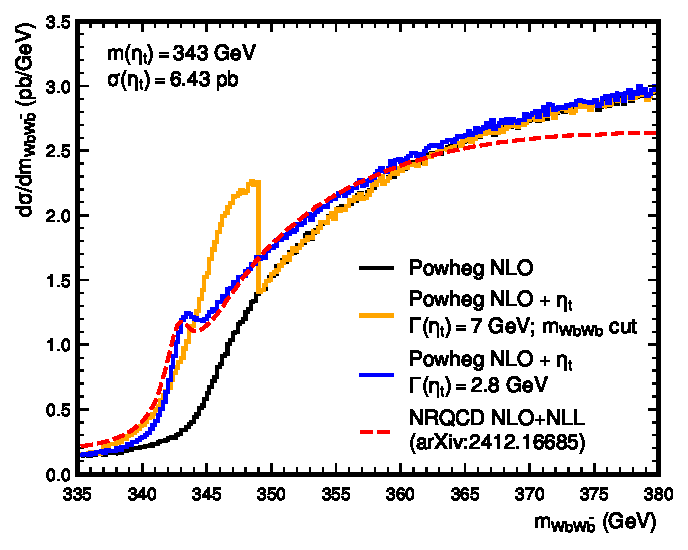
\includegraphics[width=0.8\linewidth]{figures/ah/powheg_etat_nlo.pdf}
    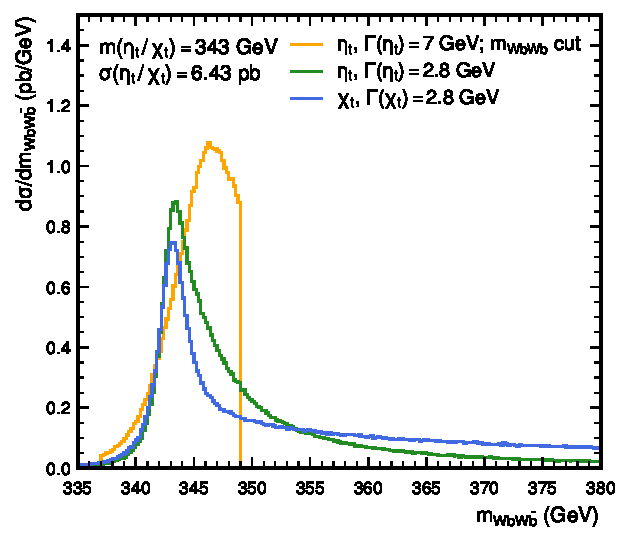
\includegraphics[width=0.49\linewidth]{figures/ah/etat_chit_small.pdf}
    \hfill
    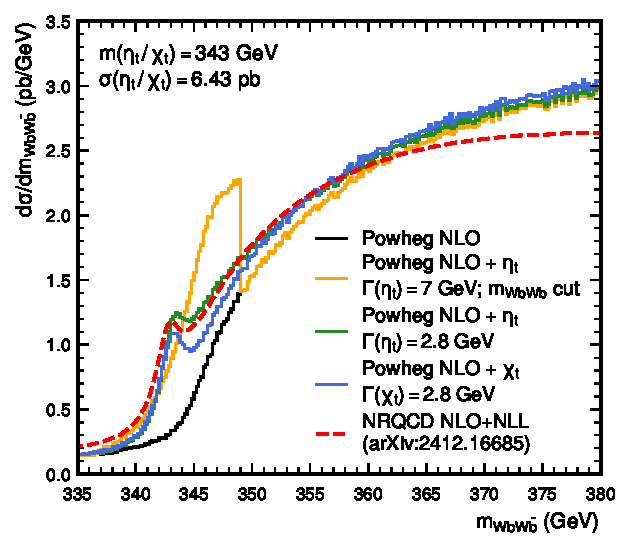
\includegraphics[width=0.49\linewidth]{figures/ah/powheg_etat_nlo_small.pdf}
    \caption{\textbf{Line shape of \etat and \chit.} The \mWWbb distribution close to the \ttbar threshold, as predicted by the \etat and \chit models on their own (left) and stacked on top of a pQCD \ttbar prediction from \powheg NLO (right, see \cref{sec:mc:ttbar}). For the orange line, the \etat width is chosen to be \SI{7}{\GeV}, and a cut on $|\mWWbb - \metat|$ is applied (\cref{eq:theory:etatparams_7gev}), while for the green line, the \etat width is chosen as \SI{2.8}{\GeV}, and no further cuts are made (\cref{eq:theory:etatparams_2p8gev}). The blue line shows \chit for a width of \SI{2.8}{\GeV}. In the right plot, all models are compared to an NRQCD prediction from \citere{Garzelli:2024uhe}.}
    \label{fig:theory:etat}
\end{figure}

The resulting \mWWbb distribution for the combination of pQCD \ttbar and \etat is shown in \cref{fig:theory:etat} at the level of hard scattering for both parameterizations, on its own as well as stacked on top of a pQCD prediction of the \ttbar continuum at NLO in QCD. The stacked distributions are compared to an NRQCD prediction from \citere{Garzelli:2024uhe}.
%In addition to the parameters given in \cref{eq:theory:etatparams}, a case with a lower width of $\Gamma_{\etat} = \SI{2.8}{\GeV}$ is also shown. 
At the level of hard scattering, the lower width of $\Gammaetat = 2 \Gammat$ agrees much better with the predicted NRQCD spectrum and avoids an unphysical discontinuity due to the \mWWbb cutoff. Thus, this parameterization will be used in this work wherever possible, i.e. in \cref{sec:ah:excess,sec:ah:limits}, though the parameterization of \cref{eq:theory:etatparams_7gev} is retained for the sake of consistency with other results in \cref{sec:ah:combination}. For more details, see these sections.

In the final stages of this work, a more involved model for \ttbar bound states was published in \citere{Fuks:2024yjj}. There, instead of simulating an additional pseudoscalar state \etat, the bound state effects are included in leading-order color-singlet \ttbar production by directly reweighting produced events with the ratio of Green's functions. This model is in principle fully predictive, i.e. it does not require fitting parameters to external calculations. However, it could not be validated in time for inclusion in the results of \cref{ch:ah}, it does not explicitly distinguish between \ttbar spin states, and it is also unclear on how to match it to the \ttbar continuum. Because of this, it is not further considered here and its investigation left for future work.
%\todo{decide on how to treat 7 and 2.8 GeV in the end}
%However, already after parton showering the difference between the cases is negligibly small due to smearing from intial and final state radiation. At detector level, this smearing is expected to increase even more due to the rather coarse experimental resolution of the \mtt reconstruction (see \cref{sec:ah:kinreco}). In general, the experimental signature of \etat will be mostly independent on the assumed mass and width in the considered ranges. Because of this, the original specification from \citere{Fuks:2021xje} is deemed sufficient and used in the remainder of this work.

While NRQCD predicts any possible \ttbar bound state contribution in pp collisions to be dominated by the \termc{1}{S}{0}{1} state, with contributions from excited states strongly suppressed, experimentally it will still be useful to compare this spin state to other possibilities. To this end, a second toy model, denoted \chit, is defined in analogy to \etat by the interaction Lagrangian

\begin{equation}
  \mathcal{L}_{\chit} = - \frac{1}{4} g_{\mathrm{gg} \chit} \chit G^{a}_{\mu \nu} \tilde{G}^{a \mu \nu} - g_{\ttbar \chit} \chit \bar{t} t
\end{equation}

\noindent where $g_{\mathrm{gg} \chit}$ and $g_{\ttbar \chit}$ are again arbitrary couplings. This Lagrangian contains a \CP-even coupling to the top quark, compared to the \CP-odd coupling in \cref{eq:theory:etatlagrangian}. It thus produces \ttbar systems in the \termc{3}{P}{0}{1} state, which is the only other possible state with $J = 0$ (cf. \cref{tab:theory:spinstates}). The free parameters of this model are again cross section, mass, and width; they are set here to the same values as for \etat in all cases\footnote{In \citere{Jiang:2024fyw}, an estimation similar to the one in \cref{sec:theory:toponium_properties} at the stable-top level results in a $\sim\SI{3}{\GeV}$ higher mass for a \term{3}{P}{0} bound state than for a \term{1}{S}{0} bound state. Similar arguments can be made based on analogies to \ccbar and \bbbar quarkonia~\cite{Barnes:2005pb}. However, it is unknown whether this would be noticeable even in the hard-scattering level spectrum due to the large smearing from the top width. It is anyway expected to be irrelevant within the experimental resolution.}. 
The resulting \mWWbb line shape is also seen in \cref{fig:theory:etat}. It shows a small peak similar to \etat at $\sim \SI{343}{\GeV}$, though it exhibits a more pronounced tail at high \mWWbb since the \term{3}{P}{0} state carries one unit of orbital angular momentum and thus favors higher top quark velocities. In \cref{sec:ah:parityscan}, the \chit model will be used in conjunction with \etat to probe the spin state of the observed excess. Other possible states, such as the vector state \termc{3}{S}{1}{1}, are not considered here and instead left for future work.

% perturbative vs non-perturbative
% quarkonia: J/Psi, Upsilon
% also for ttbar? lifetime very short - might decay before bound state forms

% formalism: pNRQCD
% what actually is that? Greens fct ? resummation in alphas/beta ?
% problem: top is unstable - width ~ binding energy, cannot neglect

% consider pseudoscalar (i.e. spin-singlet) state - largest at LHC
% color-singlet vs color-octet: only the singlet potential is attractive
% --> color-octet contributions dont give resonances
% can get gq -> singlet or even qq -> singlet in NLO, but small

% Predicted: binding energy ~ 2 GeV

% difficulties: how to match to relativistic regime?
% how to treat soft gluon emissions ?
% how to treat off-shell tops / interference with tW / WWbb ?

% mass resolution at LHC is poor - dont need details of the spectrum
% --> model as generic pseudoscalar state eta_t coupling directly to gg and ttbar - this is just a toy model
% note that seperation ``ttbar'' vs ``etat'' is nonphysical
% i.e. parametrize the enhancement through bound-state effects by etat


\section{Beyond the Standard Model}
\label{sec:theory:bsm}

The Standard Model, greatly successful as it is at describing the results of collider experiments so far, is nonetheless known to be incomplete. In fact, there exist several experimental results which cannot be explained by SM predictions, such as the observation of dark matter in many astrophysical contexts~\cite{Bertone:2004pz,Porter:2011nv,Arbey:2021gdg}, the observed matter-antimatter asymmetry in the universe~\cite{Dine:2003ax,Canetti:2012zc}, or the observed masses of the neutrinos~\cite{deGouvea:2016qpx,Dev:2023iyn}. 

In addition, the SM is plagued by several theoretical challenges that will likely not be overcome without major modifications to the theory. Chief among these is the unification of the forces of the SM - the electroweak and strong interactions - with gravity as described by General Relativity, which is not included in the SM at all. Doing so has proven extremely challenging, and no fully consistent unified theory of all forces is known yet. Further open questions are, for example, the hierarchy or naturalness problem~\cite{Nelson:1985,Koren:2020pio,Craig:2022eqo} or the strong \CP problem~\cite{Peccei:1977hh,Peccei:1977ur}.

In order to solve these problems in a satisfactory manner, a more general theory will have to be found, which should include the SM as its low-energy limit. In many cases, this will result in additional as of yet undiscovered particles. There is a multitude of such Beyond the Standard Model (BSM) extensions, each attacking different parts of the problems, and one of the major tasks of particle physics is to explore which parts of the parameter space of these models can be probed with the current experiments.

This work, in particular, aims to probe models predicting new, heavy spin-0 states coupling strongly to the top quark. 
Such models are interesting for several reasons: extensions of the Higgs sector of the SM (cf. \cref{sec:theory:higgs}) are commonly proposed to solve e.g. the naturalness problem of the SM, and usually contain additional scalar particles with Yukawa interactions~\cite{Branco:2011iw,Huitu:2019,Muhlleitner:2017dkd}. 
Additional scalars could also be mediators between the SM and dark matter~\cite{DMLHC:2015,Arina:2016}, and in certain cases could even solve the strong \CP problem (\cite{Dimopoulos:2016lvn,Gherghetta:2016fhp}, cf. \cref{sec:theory:alps}).

In \cref{sec:theory:ah}, the effect of additional scalars in the \pptt process are outlined in a generic fashion.
Following that, two explicit realizations of such models are discussed, namely the Two-Higgs Doublet Model (2HDM) (\cref{sec:theory:twohdm}) and Axion-Like Particle (ALP) models (\cref{sec:theory:alps}).

\subsection{Heavy scalars in \ttbartitle production}
\label{sec:theory:ah}

Consider an unspecified BSM extension predicting (possibly among others) a massive spin-0 state $\Phi$ coupling to top quarks via a Yukawa interaction. In the absence of couplings to other particles, the Lagrangian of such a state can be written as~\cite{Maltoni:2024tul}

\begin{equation}
\label{eq:theory:lag_ah}
    \mathcal{L}_{\Phi} = \, \frac{1}{2} (\partial_\mu \Phi ) (\partial^\mu \Phi ) +\frac{m_{\Phi}^2}{2} \Phi^2 
    + g_{\mathrm{\Phi \bar{t} t}} \frac{\mt}{v} \bar{t} \Phi \left( \cos{\alpha} + i \gamma_5 \sin{\alpha} \right) t .
    %+ i  \gAtt \, \frac{\mt}{v} \bar t  \gamma_5 \, t  \, \Phi 
    %-  \gHtt \, \frac{\mt}{v} \bar t \, t  \, \Phi .
\end{equation}

\noindent where $m_\Phi$ is the mass of the new state and $g_{\mathrm{\Phi \bar{t} t}}$ is a coupling modifier, scaled to the SM Higgs-top Yukawa coupling with the SM Higgs vacuum expectation value $v$. The phase $\alpha$ is a free parameter determining the \CP structure of the $\Phi \bar{t} t$ coupling: For $\alpha = 0$, the coupling is purely \CP-even or scalar, while for $\alpha = \pi/2$, the coupling is purely \CP-odd or pseudoscalar. Intermediate values for $\alpha$ will cause \CP-mixed couplings, which in general will result in  \CP violation in processes involving top quarks. Possible experimental indicators of such \CP violation in \pptt are e.g. discussed in \citere{Bernreuther:2017yhg}.

\begin{figure}[!t]
    \centering
    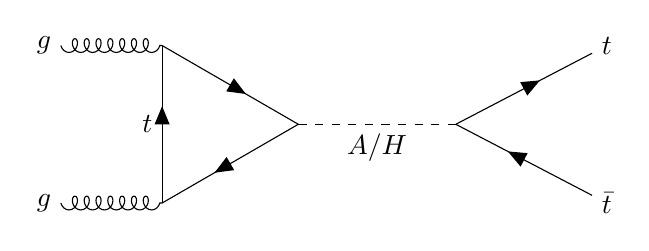
\begin{tikzpicture}[baseline=(current bounding box.center)]
      \begin{feynman}
        \vertex (i1) {\(g\)};
        \vertex [below=2.0 cm of i1] (i2) {\(g\)};
        \vertex [right=1.5 cm of i1] (a);
        \vertex [right=1.5 cm of i2] (b);
        \vertex [below right=1.0 cm and 1.73 cm of a] (c);
        \vertex [right=2.0 cm of c] (d);
        \vertex [right=5.46 cm of a] (f1) {\(t\)};
        \vertex [right=5.46 cm of b] (f2) {\(\bar{t}\)};
        \diagram* {
          (i1) -- [gluon] (a),
          (i2) -- [gluon] (b),
          (c) -- [anti fermion] (a) -- [anti fermion, edge label'=\(t\)] (b) -- [anti fermion] (c),
          (c) -- [scalar, edge label'=\(A/H\)] (d),
          (f1) -- [anti fermion] (d) -- [anti fermion] (f2)
        };
      \end{feynman}
    \end{tikzpicture}
    \caption{\textbf{Feynman diagram for $\mathrm{gg \rightarrow A/H \rightarrow \ttbar}$.} Only the leading-order gluon fusion diagram is shown, with a top quark running in the loop.}
    \label{fig:theory:ggAH}
\end{figure}

In the scope of this work, only the \CP-conserving cases of $\Phi$ are considered. For convenience, the pure pseudoscalar case will in the following be called A, while the pure scalar case will be called H.

Similar to the SM Higgs boson, the most important production channel of either state at the LHC will be through loop-induced gluon fusion, followed by associated production with either \ttbar or a single top quark. Only the former is considered here; experimental searches for the latter case can be found e.g. in \citere{CMS:EXO-22-014-PAS}. Furthermore, the decay of the new state will depend on its mass: For low masses, the particle will decay either through loop-induced couplings to e.g. gg or $\gamma \gamma$ or, if present, through couplings to other SM or BSM particles than the top quark. For masses of $\mAH > 2 \mt$, however, the decay to \ttbar is kinematically allowed and will in many cases be dominant due to the large Yukawa coupling. In this case, the process $\mathrm{gg \rightarrow A/H \rightarrow \ttbar}$ will lead to the same final state as SM \ttbar production, as illustrated in \cref{fig:theory:ggAH}. This process will be considered in more detail in the rest of this chapter, and one of the main results of this thesis is an experimental search for such a signature (\cref{ch:ah}).



\begin{figure}[ht!]
    \centering
    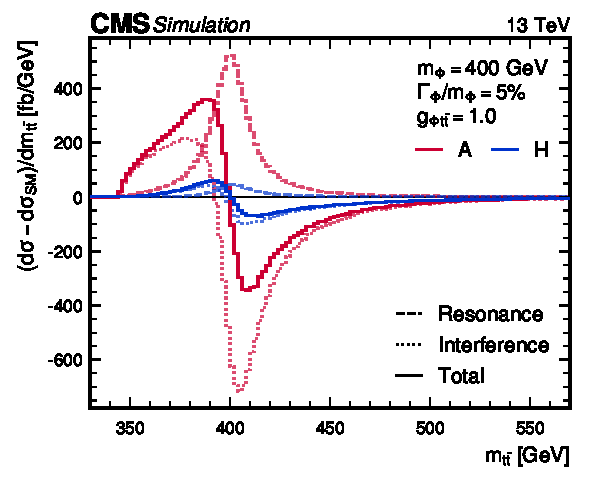
\includegraphics[width=0.49\linewidth]{figures/ah/ah_xs/ahspectrum_400.pdf}
    \hfill
    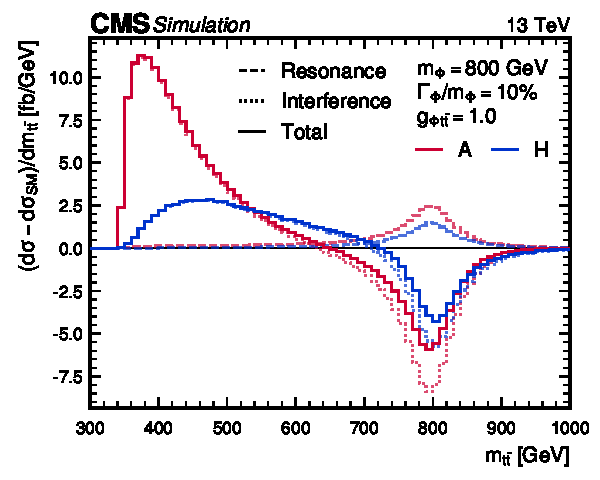
\includegraphics[width=0.49\linewidth]{figures/ah/ah_xs/ahspectrum_800.pdf}
    \caption{\textbf{Differential cross sections for $\mathrm{pp} \rightarrow \mathrm{A/H} \rightarrow \ttbar$.} The proton-proton differential cross section as a function of the invariant \ttbar mass, with the SM prediction subtracted, for $\mAH = \SI{400}{GeV}$, $\wAH/\mAH = 5\%$(left) and $\mAH= \SI{800}{\GeV}$, $\wAH/\mAH = 10\%$ (right) as well as for A (red) and H (blue), at a coupling modifier of $\gAHtt = 1$. The resonance and interference components as well as their sum are shown as dashed, dotted and solid lines, respectively. They are calculated from same the Monte Carlo simulation samples described in \cref{sec:ah:datasets}.}
    \label{fig:theory:ahxs}
\end{figure}

\cref{fig:theory:ahxs} shows the predicted differential cross sections of this model in terms of \mtt, the invariant mass of the \ttbar pair, for different A/H masses. The cross section is shown as the difference to the SM prediction at the level of the hard scattering and at LO in QCD. It can be seen that the total effect of A and H is a very distinct peak-dip structure around the A/H mass. This is because the $\mathrm{gg \rightarrow A/H \rightarrow \ttbar}$ production channel interferes with SM $\mathrm{gg \rightarrow \ttbar}$ production, which leads to deficits in certain regions of phase space due to destructive interference. For high A/H masses, there is an additional broad peak at low masses of \mtt. This originates from the gluon PDF, which is steeply increasing for small parton momentum fractions, corresponding to low \mtt, and thus compensates the suppression by the off-shell A/H at low \mtt for the A/H-SM interference.

A further consequence of the interference is that the differential cross section scales non-linearly with the coupling modifiers \gAtt and \gHtt. The dependence (for arbitrary observables) can be parameterized as 

\begin{equation}
\label{eq:theory:ahxs}
    d \sigma = d \sigma^{\mathrm{SM}} + \gAHtt^2 \, d \sigma^{\mathrm{int}} + \gAHtt^4 \, d \sigma^{\mathrm{res}}
\end{equation}

\noindent where the superscripts ``SM", ``int'' and ``res'' refer to the SM, SM-A/H interference, and resonant A/H contributions, respectively.

\begin{figure}[ht!]
    \centering
    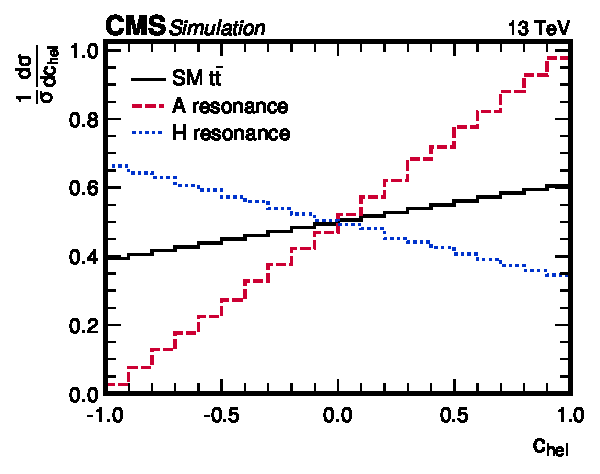
\includegraphics[width=0.49\linewidth]{figures/ah/chel_lhe_paper.pdf}
    \hfill
    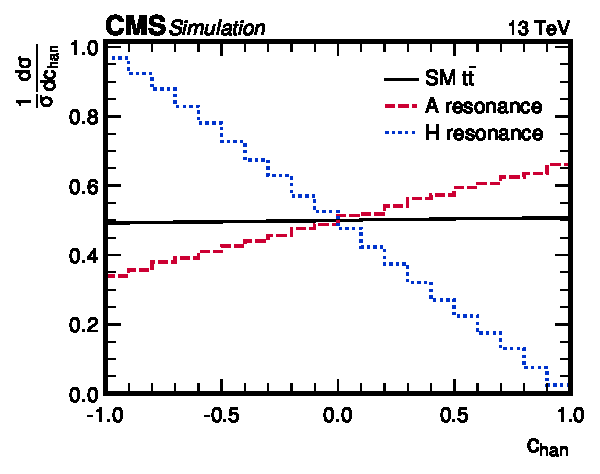
\includegraphics[width=0.49\linewidth]{figures/ah/chan_lhe_paper.pdf}
    \caption{\textbf{Distributions of \chel and \chan for $\mathrm{A/H} \rightarrow \ttbar$.} The differential cross sections as a function of \chel (left) and \chan (right) for A (red), H (blue) and the SM (black) for comparison~\cite{CMS:HIG-22-013}. They are calculated from same the Monte Carlo simulation samples described in \cref{sec:ah:datasets}.}
    \label{fig:theory:ah_chelchan}
\end{figure}

In addition to the \mtt spectrum, an A/H contribution is also expected to modify the spin state of the \ttbar system. As a single spin-0 particle, an intermediate A/H resonance has neither spin nor orbital angular momentum. Due to conservation of angular momentum, this implies that the \ttbar system will be produced in a state with $J = 0$, which leaves only the \term{1}{S}{0} and \term{3}{P}{0} states (cf. \cref{tab:theory:spinstates}).

Furthermore, the spin-0 intermediate state has positive intrinsic parity and is charge-neutral. This implies that for H, whose interaction with the top quark is \CP-even, the \ttbar system will be in the \term{3}{P}{0} state ($\CP = +1$, cf. \cref{tab:theory:spinstates}). For A, on the other hand, the interaction is \CP-odd, leading to the \term{1}{S}{0} state ($\CP = -1$). As a result, the processes $\mathrm{gg \rightarrow A \rightarrow \ttbar}$ and $\mathrm{gg \rightarrow H \rightarrow \ttbar}$ always produce pure spin singlet and spin triplet states, respectively.

%separately $\mathcal{C}$- and $\mathcal{P}$-conserving, the \ttbar system will have quantum numbers of $\mathcal{C} = +1$ and $\mathcal{P} = +1$, which is true for the \term{3}{P}{0} state. For A, on the other hand, the interaction is maximally $\mathcal{P}$-violating, leading to quantum numbers of $\mathcal{C} = +1$ and $\mathcal{P} = -1$, which matches the \term{1}{S}{0} state. As a result, the process $\mathrm{gg \rightarrow A \rightarrow \ttbar}$ will always produce the \term{1}{S}{0} spin singlet state, while $\mathrm{gg \rightarrow H \rightarrow \ttbar}$ will produce the \term{3}{P}{0} spin triplet state.

As explained in \cref{sec:theory:ttbarspin,sec:theory:spindensity}, the observable \chel has maximal slope $D$ for spin-singlet states, making it a good discriminator between A and the SM. For H, it can be shown that the produced triplet state instead maximizes the slope $D^{(k)}$ of the observable \chan, as defined in \cref{eq:theory:chan}~\cite{Maltoni:2024tul}. The distributions of both observables can be seen in \cref{fig:theory:ah_chelchan}, with the SM prediction shown as well for comparison. Both \chel and \chan will be used in the experimental search for such states presented in \cref{ch:ah}.

\subsection{Two-Higgs Doublet Model}
\label{sec:theory:twohdm}

A common class of models predicting additional scalars as discussed in \cref{sec:theory:ah} are Two-Higgs-Doublet Models (2HDMs)~\cite{Lee:1973iz,Branco:2011iw}. In these models, there are two complex $SU(2)$ Higgs doublets with eight degrees of freedom in total (as opposed to a single doublet in the SM), which after electroweak symmetry breaking results in five physical states (compare \cref{sec:theory:higgs}). Such a structure for the Higgs sector arises, for example, in many supersymmetric models~\cite{Haber:1984rc} or axion models~\cite{Kim:1986ax}.

In general, 2HDMs can include \CP-violating interactions (similar to \cref{sec:theory:ah}) as well as flavor-changing neutral currents (FCNCs). Both of these phenomena are experimentally well constrained, and so it makes sense to restrict oneself to \CP- and flavor-conserving limits. Doing so leads to definite quantum numbers of the five physical scalar states of the 2HDM: two neutral scalar (\CP-even) states h and H, a neutral pseudoscalar (\CP-odd) state A, and two charged states $\mathrm{H}^+$ and $\mathrm{H}^-$. Usually, the state h is identified with the SM Higgs boson at a mass of \SI{125}{\GeV}. Then, the two other neutral states H and A - if massive enough - could play the role of additional Higgs bosons decaying to \ttbar as discussed in \cref{sec:theory:ah}.

Depending on the nature of the discrete symmetry that is used to impose flavor conservation, there can be different types of 2HDMs, which differ in the structure of the couplings to the SM. No particular 2HDM type is assumed in this work, and the results of \cref{ch:ah} are instead presented in terms of the generic model of \cref{sec:theory:ah}.

\subsection{Axion-Like Particles}
\label{sec:theory:alps}

Another very generic class of BSM scalars relevant to the \pptt process are axions and Axion-Like Particles (ALPs), denoted here as $a$. 
Axions were originally conceived as solutions to the strong \CP problem~\cite{Peccei:1977hh,Peccei:1977ur,Weinberg:1977ma,Wilczek:1977pj}, which is a result of the non-trivial vacuum structure of QCD. When deriving the effective QCD Lagrangian, the presence of certain classes of topological solutions to the classical Yang-Mills equations leads to an additional \CP-violating term~\cite{DiLuzio:2020wdo}

\begin{equation}
\label{eq:theory:strongcp}
    \mathcal{L}^{QCD} \supset \theta \frac{\alphas}{8 \pi} G^{a}_{\mu \nu} \tilde{G}^{a \mu \nu},
\end{equation}

\noindent where $G^{a}_{\mu \nu}$ is again the gluon field strength and $\tilde{G}^{a}_{\mu \nu}$ its dual. The coefficient $\theta$ of this term is a free parameter in the range $[0,2\pi]$, with no particular value preferred from first principles. However, experimentally, no \CP violation in QCD has been observed, and $\theta$ is strongly bounded at $|\theta| \leq 10^{-10}$ (the strongest bounds coming from measurements of the electric dipole moment of the neutron~\cite{DiLuzio:2020wdo,Pendlebury:2015lrz,Abel:2020pzs}). 
The fact that \textit{a priori} the angle $\theta$ can take any value, but is bounded this strongly from the experiment, is called the strong \CP problem-
%The strong \CP problem thus consists of explaining why the \CP-violating $G^{a}_{\mu \nu} \tilde{G}^{a \mu \nu}$ term vanishes.

A possible natural solution of this problem is to introduce a new spin-0 BSM particle $a$, called the axion~\cite{Weinberg:1977ma,Wilczek:1977pj}, with a Lagrangian~\cite{DiLuzio:2020wdo}
%The most prominent way to solve the strong \CP problem is by introducing a new real scalar field $a$, the axion field, with a Lagrangian~\cite{DiLuzio:2020wdo}

\begin{equation}
\label{eq:theory:axionlagrangian}
    \mathcal{L}^{\mathrm{ax}} = \frac{1}{2} (\partial_\mu a) (\partial^\mu a) + \frac{\alphas}{8 \pi} \frac{a}{f_a} G^{a}_{\mu \nu} \tilde{G}^{a \mu \nu} + \text{interaction terms}
\end{equation}

\noindent where $f_a$ is called the axion scale, and all other interaction terms with SM fields are required to be invariant under a shift $a \rightarrow a + \kappa f_a$ with arbitrary $\kappa$. It can be shown that this Lagrangian, when added to the SM QCD Lagrangian including the term in \cref{eq:theory:strongcp}, leads to a global minimum at $a/f_a + \theta = 0$, so that after a field shift the \CP-violating term is absorbed in the axion-gluon coupling and no \CP violation is expected in QCD alone. This is known as the Peccei-Quinn mechanism.

In \cref{eq:theory:axionlagrangian}, the axion-gluon interaction term has dimension 5 and is thus non-renormalizable, with the cutoff scale given by $f_a$. The axion must thus be necessarily be seen as a low-energy EFT description of different physics at the higher scale $f_a$. Many different UV-complete models including axions exist~\cite{DiLuzio:2020wdo,Kim:1979if,Shifman:1979if,Dine:1981rt,Zhitnitsky:1980tq}, which lead to different interaction terms with other SM particles such as photons, electroweak bosons or massive fermions.

In this work, a focus is placed upon models which predict couplings to SM fermions, particularly the top quark. The EFT Lagrangian is parameterized in a model-independent approach as~\cite{Georgi:1986df}

\begin{equation}
\begin{split}
\label{eq:theory:alplagrangian}
    \mathcal{L}^{\mathrm{ALP}} =& \, \frac{1}{2} (\partial_\mu a) (\partial^\mu a)
    + \frac{m_a^2}{2} a^2
    - c_G \frac{a}{f_a} G^{a}_{\mu \nu} \tilde{G}^{a \mu \nu}
    - c_B \frac{a}{f_a} B_{\mu \nu} \tilde{B}^{\mu \nu} \\
    & - c_W \frac{a}{f_a} W^{a}_{\mu \nu} \tilde{W}^{a \mu \nu}
    - \sum_f c_f \frac{\partial^\mu a}{f_a} \bar{\Psi}_f \gamma_\mu \Psi_f ,
\end{split}
\end{equation}

\noindent where the index $f$ runs over the SM fermions, $\Psi_f$ are the fermion fields, $B_{\mu \nu}$ and $W^{a}_{\mu \nu}$ are the EW boson fields before symmetry breaking, and the free parameters are the scale $f_a$, the mass $m_a$, and the couplings to gluons $c_G$, to EW bosons $c_B$ and $c_W$ and to fermions $c_f$ (where no flavor mixing was assumed). This Lagrangian, depending on the choice of the free parameters, might or might not correspond to a UV-complete model and solve the strong \CP problem. Because of this, the field $a$ is here called an Axion-Like Particle. Even when it does not correspond to a true axion, it might be a physically well-motivated extension of the SM, e.g. as a dark matter candidate or mediator.

In the ALP-fermion interaction term in \cref{eq:theory:alplagrangian}, the shift symmetry of $a$ is directly manifest since it only depends on the derivative of $a$. However, by employing the equations of motion for $a$ as well as the Higgs mechanism, one can rewrite \cref{eq:theory:alplagrangian} with a Yukawa-like interaction instead~\cite{Brivio:2017ije,Bauer:2020jbp,Bonnefoy:2022rik}. Dropping the EW bosons and fermions other than the top quark leads to

\begin{equation}
\label{eq:theory:alplagrangian2}
    \mathcal{L}^{\mathrm{ALP}} = \, \frac{1}{2} (\partial_\mu a) (\partial^\mu a)
    + \frac{m_a^2}{2} a^2
    - \cG \frac{a}{f_a} G^{a}_{\mu \nu} \tilde{G}^{a \mu \nu}
    + i \ct \mt \frac{a}{f_a} \bar{t} \gamma^5 t .
\end{equation}

Performing this basis change induces an additional ALP-gluon coupling term (in general dependent on the other SM couplings), which was absorbed by redefining the Wilson coefficient from $c_G$ to \cG as~\cite{Bauer:2020jbp,Jeppe:2024sxt}

\begin{equation}
  \cG = c_G + \frac{\alphas}{8 \pi} \ct
\end{equation}

\noindent where couplings to EW bosons and other fermions were again dropped. This basis will be used in the remainder of this work. 

\begin{figure}[!t]
    \centering
    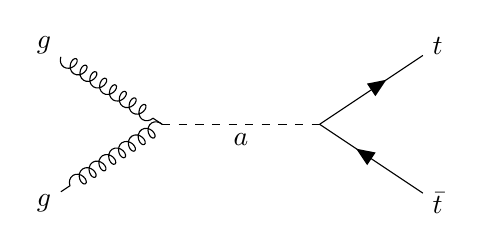
\begin{tikzpicture}[baseline=(current bounding box.center)]
      \begin{feynman}
        \vertex (i1) {\(g\)};
        \vertex [below=2.0 cm of i1] (i2) {\(g\)};
        \vertex [below right=1.0 cm and 1.5 cm of i1] (c);
        \vertex [right=2.0 cm of c] (d);
        \vertex [right=5 cm of i1] (f1) {\(t\)};
        \vertex [right=5 cm of i2] (f2) {\(\bar{t}\)};
        \diagram* {
          (i1) -- [gluon] (c) -- [gluon] (i2),
          (c) [dot] -- [scalar, edge label'=\(a\)] (d),
          (f1) -- [anti fermion] (d) -- [anti fermion] (f2)
        };
      \end{feynman}
    \end{tikzpicture}
    \quad \quad
    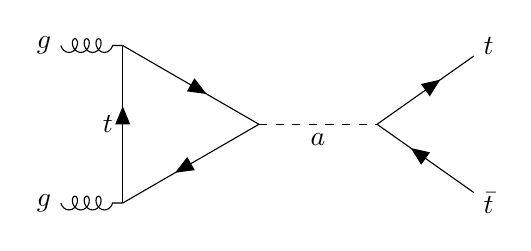
\begin{tikzpicture}[baseline=(current bounding box.center)]
      \begin{feynman}
        \vertex (i1) {\(g\)};
        \vertex [below=2.0 cm of i1] (i2) {\(g\)};
        \vertex [right=1 cm of i1] (a);
        \vertex [right=1 cm of i2] (b);
        \vertex [below right=1.0 cm and 1.73 cm of a] (c);
        \vertex [right=1.5 cm of c] (d);
        \vertex [right=4.46 cm of a] (f1) {\(t\)};
        \vertex [right=4.46 cm of b] (f2) {\(\bar{t}\)};
        \diagram* {
          (i1) -- [gluon] (a),
          (i2) -- [gluon] (b),
          (c) -- [anti fermion] (a) -- [anti fermion, edge label'=\(t\)] (b) -- [anti fermion] (c),
          (c) -- [scalar, edge label'=\(a\)] (d),
          (f1) -- [anti fermion] (d) -- [anti fermion] (f2)
        };
      \end{feynman}
    \end{tikzpicture}
    \caption{\textbf{Feynman diagrams for $gg \rightarrow a \rightarrow \ttbar$.} The left diagram corresponds to the gluon-ALP contact interaction and scales with $\cG\ct$, while the right diagram shows the top quark loop and scales with $\ct^2$.}
    \label{fig:theory:ggALP}
\end{figure}

It can be seen by comparing \cref{eq:theory:alplagrangian2} to \cref{eq:theory:lag_ah} that the ALP-top coupling has the exact same structure as the generic \CP-odd boson introduced in \cref{sec:theory:ah}. Thus, if the ALP is heavy enough to be produced at the LHC and decay to \ttbar, it can be searched for in \ttbar final states similarly to the generic pseudoscalar A. Such heavy ALP masses can  be reached naturally and serve as solutions to the strong \CP problem e.g. in UV models containing extra non-Abelian gauge groups, resulting in containing forces with large containment scales~\cite{Rubakov:1997vp,Holdom:1982ex,Dimopoulos:2016lvn,Gherghetta:2016fhp}.

If, in addition, the ALP couplings also satisfy $\cG = 0$, the two Lagrangians in \cref{eq:theory:alplagrangian2,eq:theory:lag_ah} are identical, and all conclusions drawn on A can be directly transferred to the ALP. On the other hand, if $\cG \neq 0$, an additional production diagram involving a gluon contact interaction becomes available, as depicted in \cref{fig:theory:ggALP} (left). A phenomenological study characterizing both cases in detail forms the core of \cref{ch:alps} of this work.

% ALPs: another model of generic spin-0 particles
% motivation: axions: solve the strong \CP problem
% axions are restricted to certain masses vs couplings
% have U(1) shift symmetry
% ALPs: all particles with this shift symmetry - very generic
% not a UV complete theory: dimension 5 operators, ALP scale
% explicit realizations (maybe)
% large mass range allowed
% ch 8 focus on large masses, top couplings

\chapter{Experimental methods}
\label{ch:methods}

\section{The Large Hadron Collider}
\label{sec:methods:lhc}

At the time of writing, the Large Hadron Collider~\cite{Bruning:2004ej} at CERN is the largest and most powerful particle accelerator in the world. Located underground at the border of France and Switzerland close to Geneva, it consists of two circular beamlines of roughly 27~km circumference in which proton bunches are accelerated and collided. Superconducting magnets, cooled with liquid helium to temperatures of around 4~K, generate magnetic fields of over 8~T to keep the protons on their circular orbit, and similarly superconducting electromagnetic radio-frequency cavities accelerate the protons to beam energies up to 7~TeV. When operating as designed, around 2800 proton bunches per beam containing $3\times10^{14}$ protons total are present in the beamline simultaneously, revolving with a frequency of about 11.245~kHz. From this, peak instantaneous luminosities of about \SI{20}{\kilo\hertz\per\micro\barn} can be reliably reached. Alternatively, the LHC can also collide heavy ions, such as lead or oxygen, instead of protons.

\begin{figure}[!t]
    \centering
    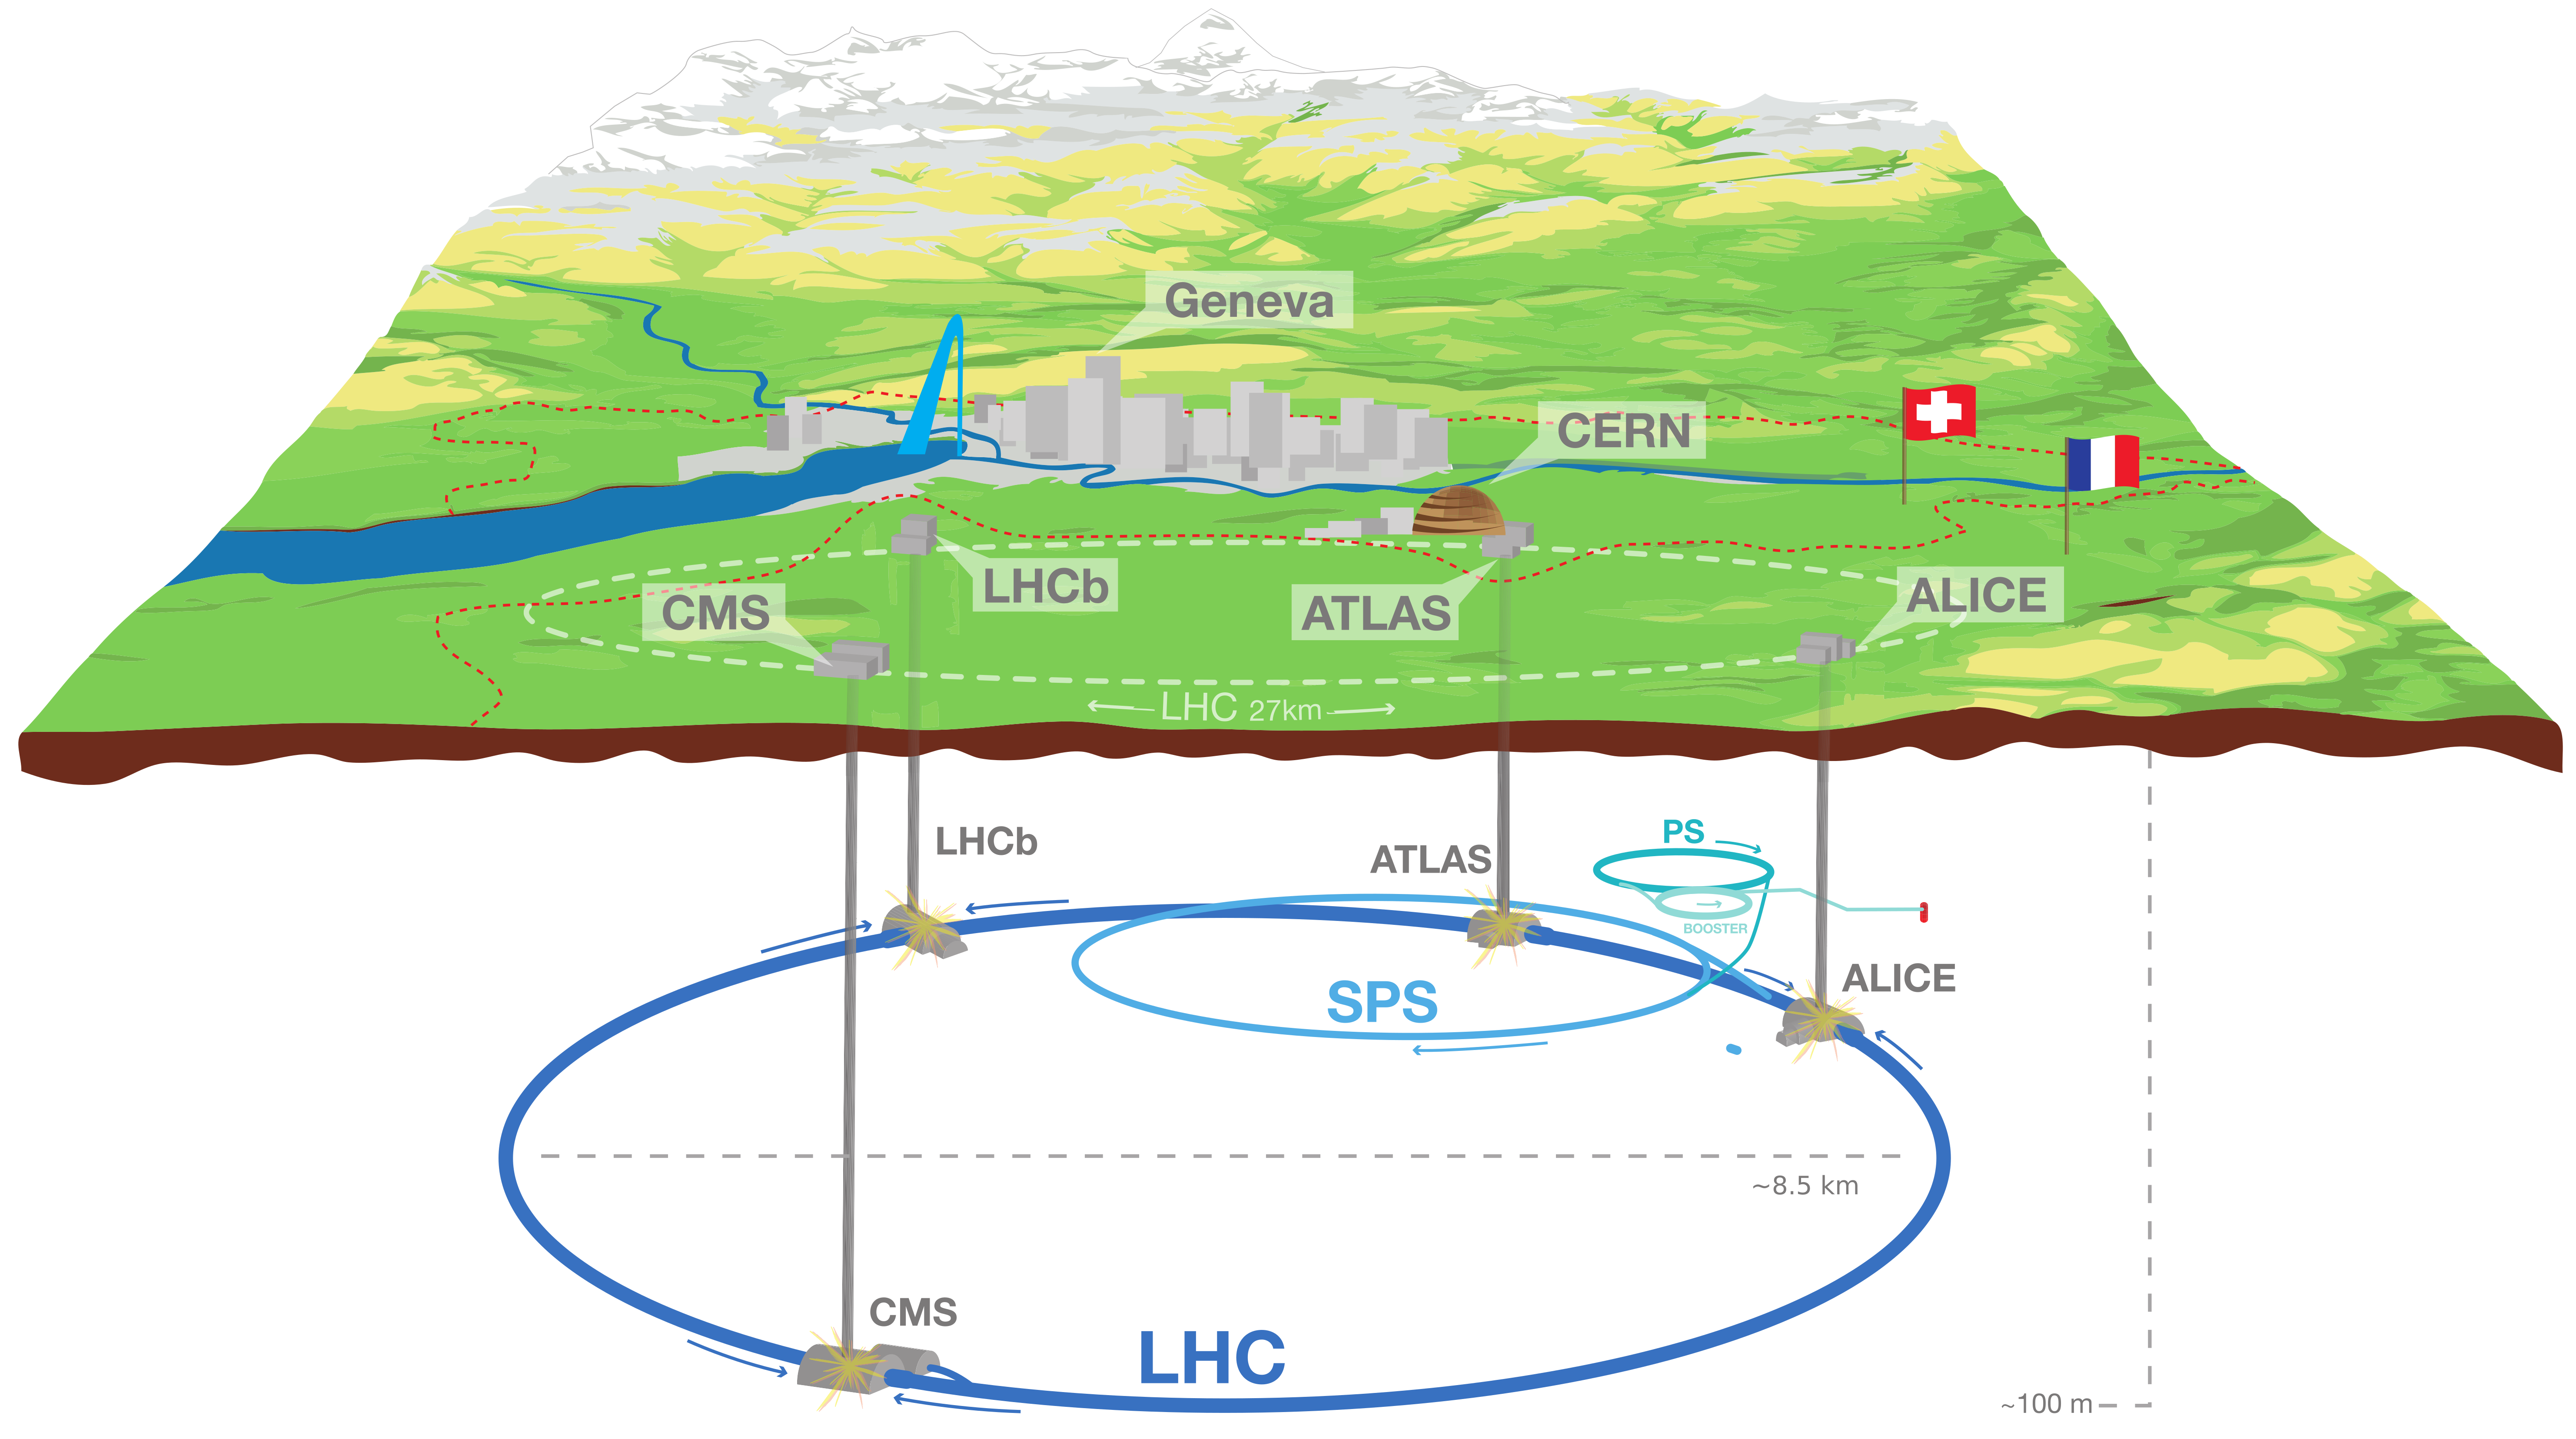
\includegraphics[width=\textwidth]{figures/lhc_sketch.pdf}
    \caption{\textbf{The Large Hadron Collider}. A sketch of the LHC and its location in Geneva, Switzerland, including its two pre-accelerators PS and SPS as well as the four large experiments ATLAS, CMS, ALICE and LHCb. \textit{Figure taken from \citere{LHC:sketch}}.}
\end{figure}

There are four large experiments making use of the colliding beams at the LHC, located at the four interaction points. The two larger of these are ATLAS~\cite{ATLAS:2008xda} and CMS~\cite{CMS:2008xjf}, both of which are general-purpose experiments intended to study all aspects of the Standard Model in proton-proton collisions. The work of thesis was performed as part of the CMS Collaboration, and so the CMS experiment is described in \cref{sec:methods:cms} in more detail. The two smaller experiments, on the other hand, are specialized for certain tasks, namely the study of B physics and exotic hadrons for LHCb~\cite{LHCb:2008vvz} and the study of heavy-ion collisions for ALICE~\cite{ALICE:2008ngc}.

The data taken at the LHC so far can be divided into three Runs. Run~1 lasted from 2010--2012, during which the LHC operated at center-of-mass energies of 7 and 8~TeV, significantly below the original target values, and yielded a total integrated luminosity of about \SI{29}{\fbinv}. It is this data that led to the original discovery of the Higgs boson. Following this, after two years of pause, Run~2 resumed in 2015 with a center-of-mass energy of 13~TeV and lasting to 2018. Around \SI{140}{\fbinv} of data was collected during this time. This complete data set, save for the small contribution from 2015, is analyzed in \cref{ch:ah} of this thesis.

Then, Run~3 of the LHC started in 2022 after another three years of pause, and is planned to last until 2026 at the time of writing. The center-of-mass energy was again increased slightly to 13.6~TeV, and in the years 2022--2024 around \SI{196}{\fbinv} have been recorded, already surpassing Run~2. In \cref{ch:ttxs} of this thesis, the very first data of Run~3, corresponding to \SI{1.21}{\fbinv} taken in July and August 2022 at CMS, are analyzed in the context of a \ttbar cross section measurement. 

In the future, it is planned to upgrade the LHC to be able to run at higher instantaneous luminosities as well as a further increased energy of 14~TeV~\cite{ZurbanoFernandez:2020cco}. The CMS detector will similarly be upgraded to replace aging components and deal with the increased pileup conditions~\cite{CMS:TDR-15-02,CMS:PRF-21-001}, and a total integrated luminosity of around \SI{3}{\abinv} is expected to be collected. In \cref{ch:alps}, among others, sensitivity projections for this luminosity are made for Axion-Like Particles decaying to \ttbar.

\section{The CMS experiment}
\label{sec:methods:cms}

The Compact Muon Solenoid experiment~\cite{CMS:2008xjf,CMS:PRF-21-001}, located at Interaction Point~5 of the LHC close to Cessy, France, is a general-purpose particle detector targeting a broad range of SM and BSM phenomena. Its main feature is a superconducting solenoid magnet creating a strong magnetic field of 3.8~T. CMS is a hermetic detector, covering almost the full solid angle in space, and is split into a \textit{barrel}, covering a range of $\abseta \lesssim 1.5$, and two forward \textit{endcaps}, covering $\abseta \gtrsim 1.5$. 
Here, $\eta = \sinh^{-1} (p_z / \pt)$ is the \textit{pseudorapidity}, which is commonly used in collider experiments to quantify the forward momenta $p_z$ of particles relative to their transverse momenta \pt.
CMS consists of several subdetectors, which are geared towards different particle types and properties.

\begin{figure}[!t]
    \centering
    \includegraphics[width=\textwidth]{figures/cms_photo.jpg}
    \caption{\textbf{Photo of the CMS detector}. A photograph of the opened CMS detector, taken during the installation of the tracker. \textit{Figure taken from \citere{CMS:detector_photo}}.}
\end{figure}

\paragraph{Subdetectors}
The innermost part of CMS is the \textit{tracker}, which is a silicon detector comprised of several layers of silicon pixel and strip sensors~\cite{CMS:2014pgm,CMSTrackerGroup:2020edz}. These record interactions with particles (``tracker hits'') shooting outwards from the interaction point in the center in three-dimensional space. Through reconstruction of the particle tracks and fits of the curvature due to the magnetic field, the tracker thus allows for the measurement of particle momenta. Furthermore, extrapolating the tracks back to their origin allows for the determination of the point of interaction, and thus for discrimination between particles arising from different proton-proton interactions. Due to the presence of the beam pipe, the tracker covers only pseudorapidities of $\abseta < 2.5$, enabling high precision momentum determination in this range only.

\begin{figure}[!t]
    \centering
    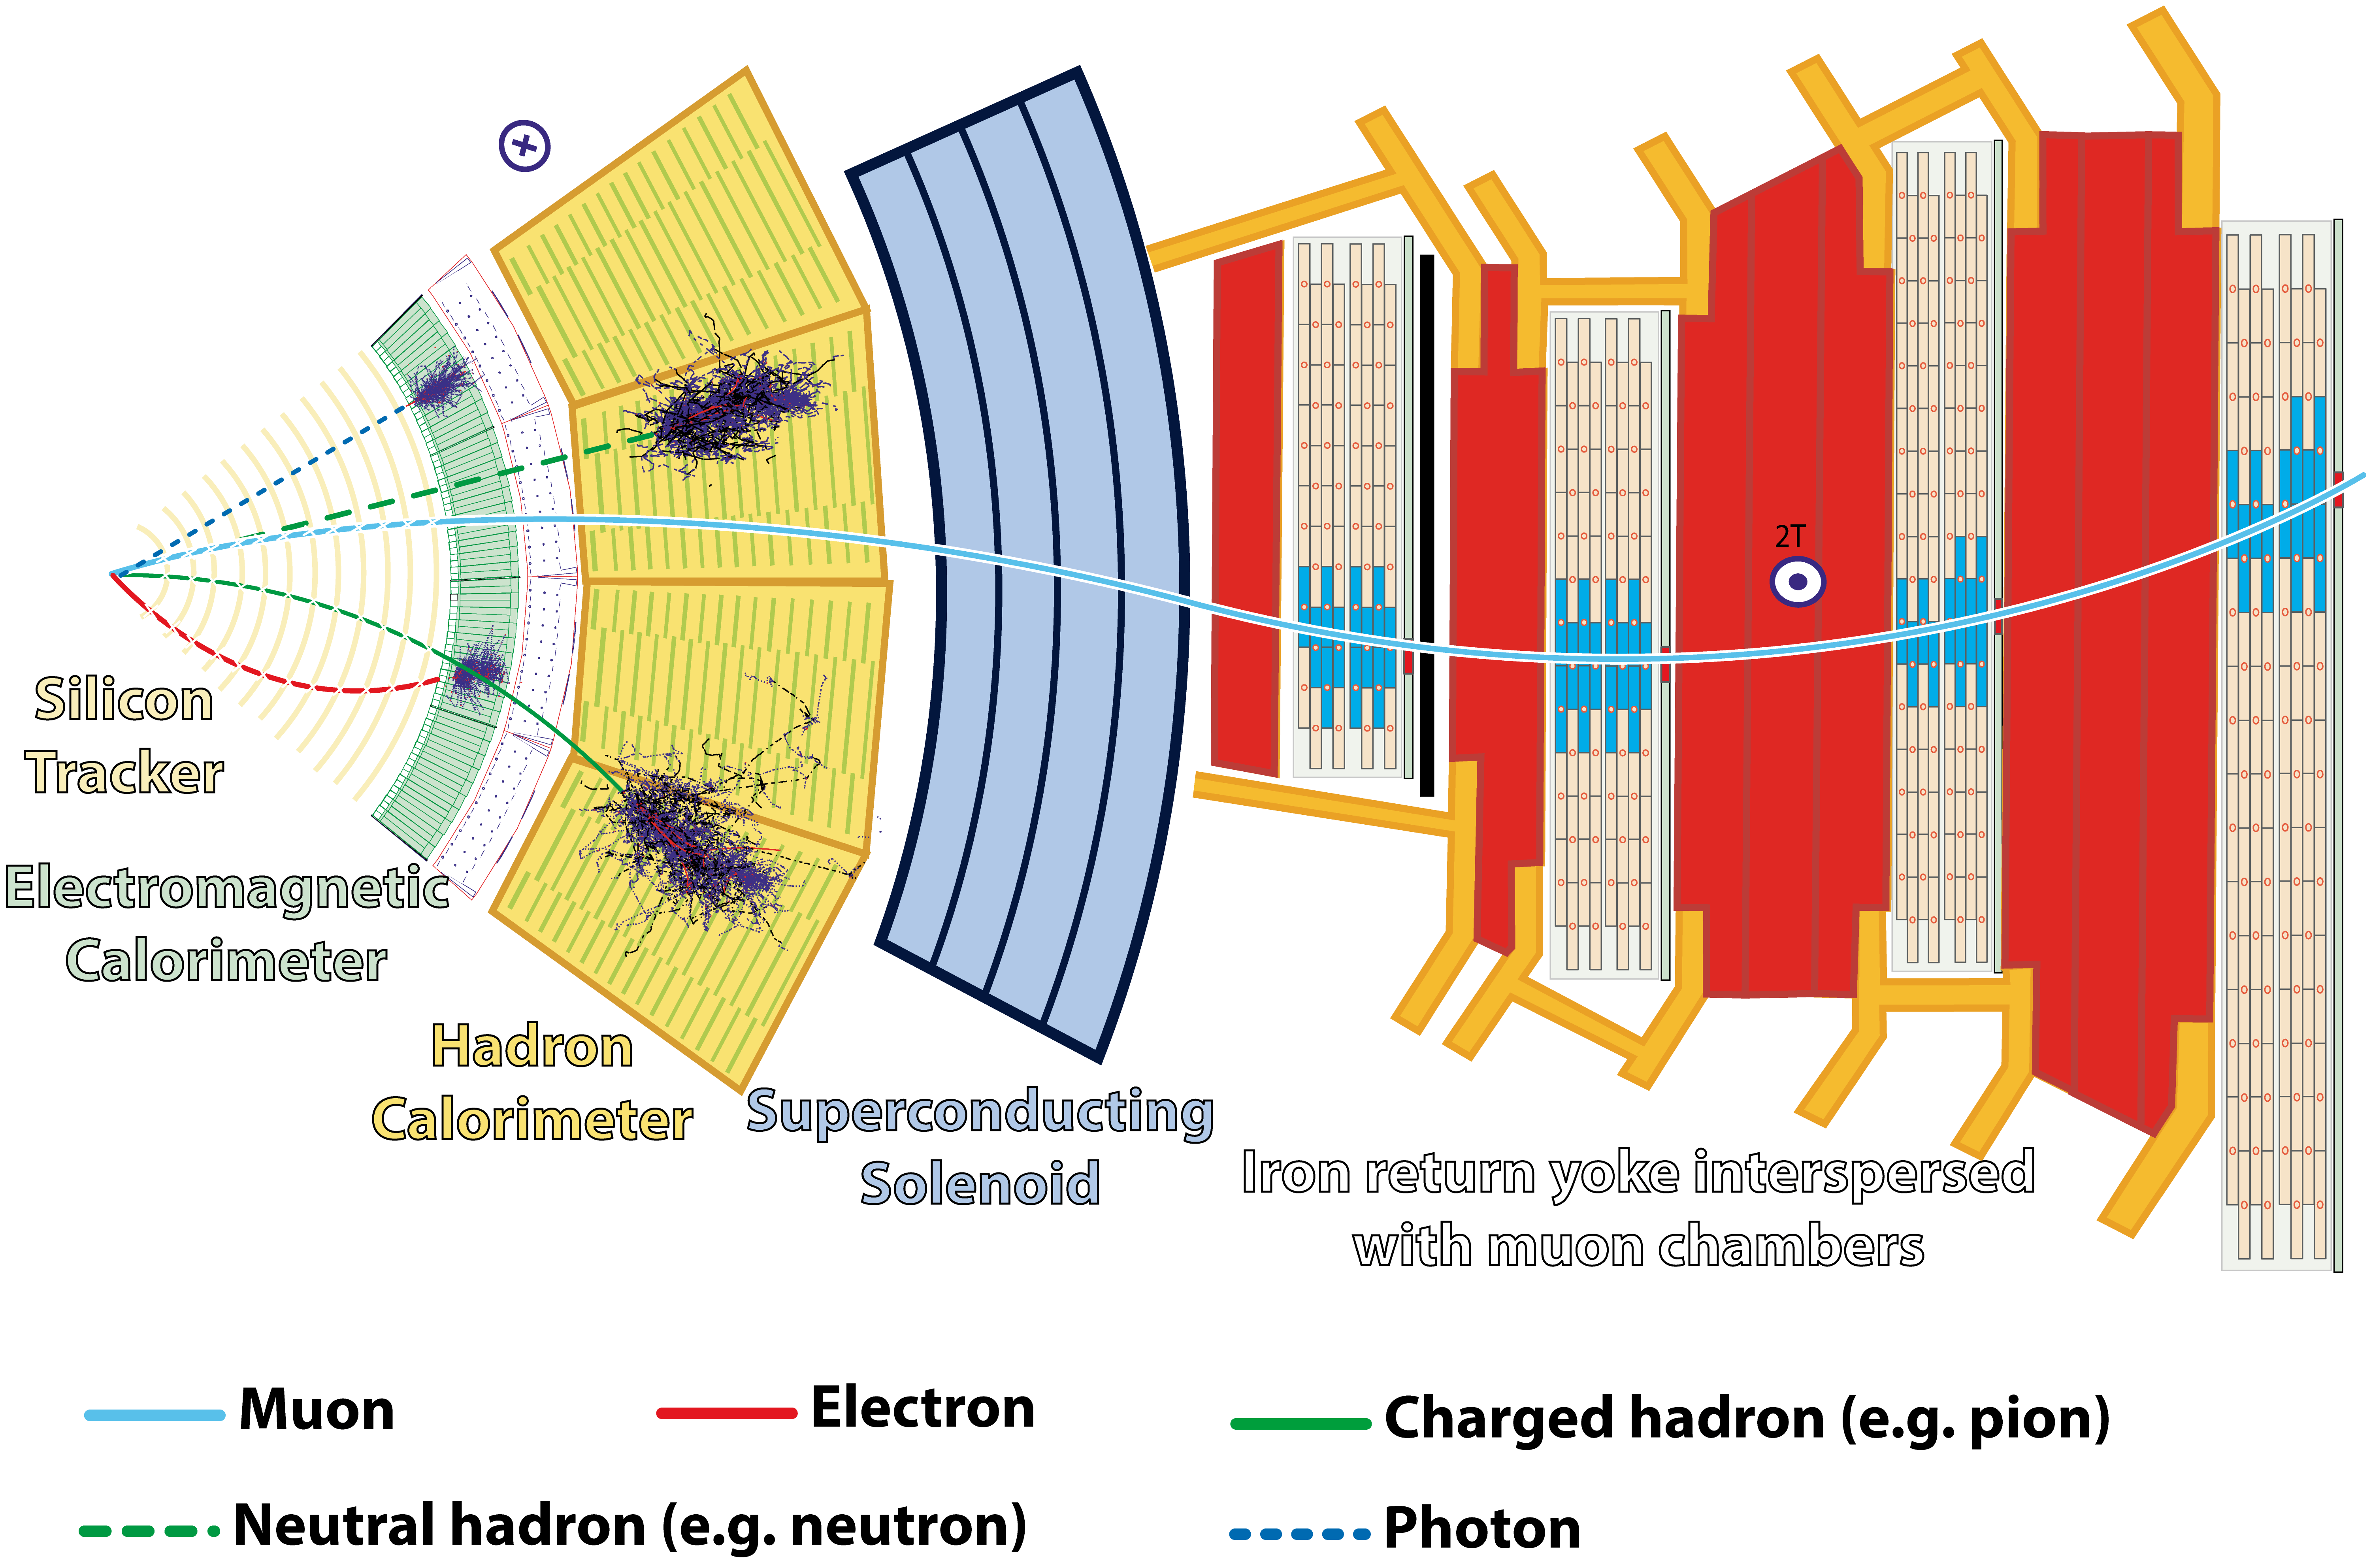
\includegraphics[width=\textwidth]{figures/cms_slice.png}
    \caption{\textbf{Sketch of the CMS subdetectors}. A cross section view of the different CMS subdetectors, with the trajectories of example particles and their interactions. \textit{Figure taken from \citere{CMS:detector_slice}}.}
\end{figure}

The second-to-innermost subdetector is the \textit{electromagnetic calorimeter} (ECAL), which is intended to measure the energy of electrons and photons~\cite{CMS:1997ysd,CMS:EGM-17-001}. It consists of transparent lead tungstate cells, in which incoming electrons or photons create electromagnetic showers leading to avalanches of electron-positron pairs and photon radiation. These are then recorded by photo diodes, and the energy of the incoming particle can be reconstructed from the amount of measured photons. Pseudorapidities of $\abseta < 1.48$ and $1.65 > \abseta < 3$ are covered for the barrel and the endcaps, respectively. The majority of electrons and photons are fully stopped in the ECAL and do not interact with the further subdetectors.

Following the ECAL, the \textit{hadronic calorimeter} (HCAL) measures the energy of charged or neutral hadrons~\cite{CMS:1997xji,CMS:2012tda}. It is a sampling calorimeter consisting of interleaved absorber plates, which initiate hadronic showers through the strong interaction with the nuclei of the material, and scintillators, which transmute the hadronic showers into photons to be detected by photodectectors. The HCAL covers $\abseta < 1.4$ and $1.4 < \abseta < 3$ for the barrel and endcaps, respectively, and additionally features a forward section ranging up to $\abseta < 5$, though the latter is not used anywhere in this work.

Surrounding the HCAL lies the superconducting solenoid, further surrounded by the final subdetector: the \textit{muon chambers}~\cite{CMS:1997iti,Pozzobon:2701333}. They are interspersed with four layers of the iron return yoke of the magnet, which confines the magnetic field. Since muons interact only sparsely with matter, they escape the calorimeters and the solenoid unhindered, and are detected in four muon subsystems working in accord at different pseudorapidities: the drift tubes ($\abseta < 1.2$), cathode strip chambers ($0.9 < \abseta < 2.4$), resistive plate chambers ($\abseta < 1.9$) and gas electron multipliers ($1.6 < \abseta < 2.4$). All of them are gas detectors, which are sensitive to the ionization of a gas when a muon passes through it, and record hits of the muon trajectory, thus allowing for a momentum measurement similar to the tracker.

\paragraph{Trigger system}
Besides the different subdetectors, a crucial part of the CMS experiment is the \textit{trigger system}~\cite{CMS-TRG-12-001}. It is necessary due to the large number of bunch crossings at the LHC, which, if they were all recorded, would produce data rates far in excess of the computational bandwidth and storage capacities available. To combat this, only events which are of physical interest should be recorded. It is the task of the trigger system to determine what these events should be.

The trigger system is split into two parts. The first is the low-level or level-one trigger (L1T)~\cite{CMS:TRG-17-001}, which is a hardware trigger consisting of custom electronics and whose inputs are directly the output signals of several of the subdetectors. It is designed to trigger on signatures consistent with specific objects, such as electrons, muons or hadronic jets, with significant energy. Since it needs to take a decision for every collision event, it only has a time interval of around \SI{4}{\micro\second} to do so, requiring purpose-built low-latency electronics. Its target is an output event rate of 100~kHz, which can be adjusted by prescaling certain trigger paths so that only a fraction of passing events is recorded.

The second part of the trigger system is the high-level trigger (HLT)~\cite{CMSTrigger:2005yhe,Varghese:20232Q}. It is a software trigger, running on a GPU-accelerated server farm directly in the CMS service cavern, on which a dedicated, speed-optimized version of the standard CMS object reconstruction algorithm is executed for each event passing the L1T. Specific triggers are then implemented as decisions based on these reconstructed trigger objects, allowing large freedom in selecting events based on the desired physics program. Typical triggers require, for example, the presence of different numbers or combinations of electrons, muons, photons, hadronic jets or missing transverse momentum. The transverse momentum thresholds and further requirements on these objects need to be adjusted so that the total trigger rate is reduced to an average of around 400~Hz. Only these events are then saved to hard drives, and kept for further analysis.

\section{Object reconstruction}
\label{sec:methods:reco}

In order to interpret the physics behind a collision event, the outputs of the subdetectors have to be translated into physics objects which can be mapped to the underlying physical particles. At CMS, this is done with a single unifying method, the Particle Flow (PF) algorithm~\cite{CMS:PRF-14-001}, which is designed to combine the information from the several subdetectors to build physics objects (called PF candidates) as appropriate. The physics objects relevant to this work are listed in the following.

\textit{Charged particle tracks} are obtained from the tracker by fitting recorded tracker hits using a $\chi^2$ minimization, and their momentum and charge are estimated from their curvature as described above~\cite{CMS:2014pgm}. 
%Information from the muon chambers is also included to identify and precisely determine the momenta of muon tracks. 
By extrapolating the tracks back to their origin, the position of vertices in space can also be determined. 
    
From this, the \textit{primary vertices} (PVs) can be found, which are the locations of the proton-proton interactions that caused the tracks in the first place. By contrast, secondary vertices arise from the decays of particles with long enough lifetime that they move a significant distance from the PV. PVs are determined by a likelihood fit to all tracks of sufficient quality~\cite{CMS:2014pgm}. In each event, the PV whose tracks show the largest \pt sum is designated the hard-scattering PV, assumed to correspond to the physical process of interest, while further PVs are due to soft-QCD pileup interactions. The number of PVs per event is thus a good measure of the amount of pileup.
    
The other main ingredient besides tracks and vertices are \textit{calorimeter clusters} from either the ECAL or the HCAL. A clustering algorithm is required here because particles typically deposit their energy in more than one calorimeter crystal.

By matching the positions of calorimeter clusters and charged particle tracks, \textit{electrons} (for the ECAL) and \textit{charged hadrons} (for the HCAL) can be constructed. The combined measurements of the momentum (from the curvature) and the deposited energy (from the calorimeter) allows for the reconstruction of the mass, and thus the identification of the particle.
For electrons, the effect of bremsstrahlung originating in the tracker volume has to be considered, usually resulting in multiple calorimeter clusters per electron (called a supercluster) which need to be combined together. Isolation criteria on the clusters are also required to veto electrons that are part of a hadronic jet (see below). 
By contrast, calorimeter clusters which do not have charged tracks are assigned to \textit{photons} (for the ECAL) or \textit{neutral hadrons} (for the HCAL). 
CMS furthermore employs algorithms to remove hadrons that are believed to originate from pileup instead of the hard-scattering vertex. In Run~2, the Charged Hadron Subtraction (CHS) method~\cite{CMS:PRF-14-001} was used for this purpose, while in Run~3, the better performing PUPPI method~\cite{Bertolini:2014bba,CMS:2020ebo} was used instead.

\textit{Muons} interact only very rarely with the calorimeter, and are instead built by directly combining charged tracks with hits in the muon chambers. In this work, muons are only considered if they match to hits in both subdetectors.

From these definitions, further high-level objects can be built. The first are \textit{hadronic jets}, which are clustered from all other PF candidates using the anti-$k_T$ algorithm with a distance parameter of $\Delta R = 0.4$~\cite{Cacciari:2008gp} (referred to as AK4 jets). This algorithm is infrared- and collinear-safe, i.e. it is insensitive to soft and/or collinear radiation in QCD, which is nonperturbative~\cite{Skands:2012ts}. It further has the advantage that the resulting jets are approximately circular in the $\varphi$--$\eta$ plane, making them experimentally intuitive to handle. Since leptons or photons can be created from electroweak decays of hadrons, these also need to be included in the jet clustering; to ensure that they are not double-counted, leptons and photons that are included in jets are not further considered as standalone objects.

Hadronic jets can further be \textit{b tagged}, that is, identified as originating from a B hadron. Since the strong interaction is flavor-conserving, the decay of B hadrons to hadrons of other flavors has to be mediated by the flavor-mixing in the weak interaction, leading to comparatively long lifetimes. B hadrons can thus be identified through secondary vertices corresponding to the B hadron decay, which can be displaced from the PV by several millimeters. In practice, machine learning-based classifiers like the \textsc{DeepJet} algorithm~\cite{DeepJet:2020} are used, which take more properties of the jet into account besides the displacement of the secondary vertex.

Finally, the \textit{missing transverse momentum} \ptmissvec can be calculated as the negative of the vectorial sum of all transverse momenta in the event~\cite{CMS:JME-17-001}. Since the initial state of a collision at the LHC has negligible transverse momentum, \ptmissvec represents the total transverse momentum of the particles that left the detector unobserved. In the SM, this is the case for neutrinos, but it could also be BSM particles such as e.g. dark matter candidates.



\chapter{Measurement of the inclusive \ttbartitle cross section at \texorpdfstring{$\sqrt{s}$}{sqrt(s)} = 13.6 TeV}
\label{ch:ttxs}

%This chapter describes the measurement of the inclusive \ttbar production cross section at the LHC at the center-of-mass energy of \sqrtsRIII. First, a motivation and overview of the analysis design will be given. Then, object and cut definitions as well as several applied corrections will be explained in detail. Finally, the likelihood fit used to extract the cross section, including all uncertainties, is described and the result discussed.

\section{Introduction}

% motivation: new com energy, possible glimpse at new physics; new run, new calibrations, top physics requires most objects -> good check of performance

% method needs to be tuned for early measurement
% special mention: lepton sf -> can be estimated in situ
% do one fit with and one without

In July 2022, the LHC officially resumed collecting data after over three years of shutdown, thereby starting LHC Run~3. It did so at a new, unprecedented center-of-mass energy of \sqrtsRIII, inviting the experiments to measure physical observables at the new energy frontier.

One important such observable is the inclusive \ttbar production cross section. It is, in essence, the total rate of top quark pair production at the LHC, integrated over the kinematic distributions of the particles produced. As mentioned in \cref{ch:theory}, the top quark has a special place in the standard model as the heaviest known elementary particle, as well as the only colored particle that decays before hadronizing. 
It is thus important for many potential BSM scenarios, such as models with additional Higgs bosons, which might couple strongly to the top quark. 
As such, measurements of top quark-related observables at the highest possible energies are attractive tests of the SM. The inclusive \ttbar production cross section, as one of the simplest top quark observables, is well suited for a first measurement at the new center-of-mass energy.

Simultaneously, restarting such a large experiment as CMS after a three-year shutdown poses many experimental challenges. Due to the change in energy, as well as physical changes in the accelerator and detector, new calibrations as well as validations of some previous calibrations are required to ensure that the detector performance is understood. An early measurement of the inclusive \ttbar cross section is well suited to serve as such a cross-check: Because of the decay chain of the top quark, a top quark measurement involves many of the different objects reconstructed at CMS, which
%, as described in Ch. \ref{sec:methods:reco}, 
allows for a check of a wide landscape of calibrations.

The measurement described in this chapter was designed specifically with these motivations in mind, and as such exhibits several novel features. Firstly, it combines events from both the dilepton and \ljets decay channels of \ttbar, categorized by lepton flavor content, combining the higher statistics of the \ljets channel with the high purity of the \emu channel and allowing to constrain uncertainties on the lepton identification efficiency directly from the data. This is done using a simultaneous maximum likelihood fit (cf. \cref{ch:stat}) to the event yields in the different categories, with experimental and theoretical uncertainties treated as nuisance parameters.

Secondly, the events are additionally categorized by their number of b-tagged jets (cf. \cref{sec:methods:reco}), which similarly allows for an in-situ measurement of the b-tagging efficiencies. This averts needing to wait for external b-tagging calibrations, allowing for a measurement as early as possible.

\begin{figure}[!t]
    \centering
    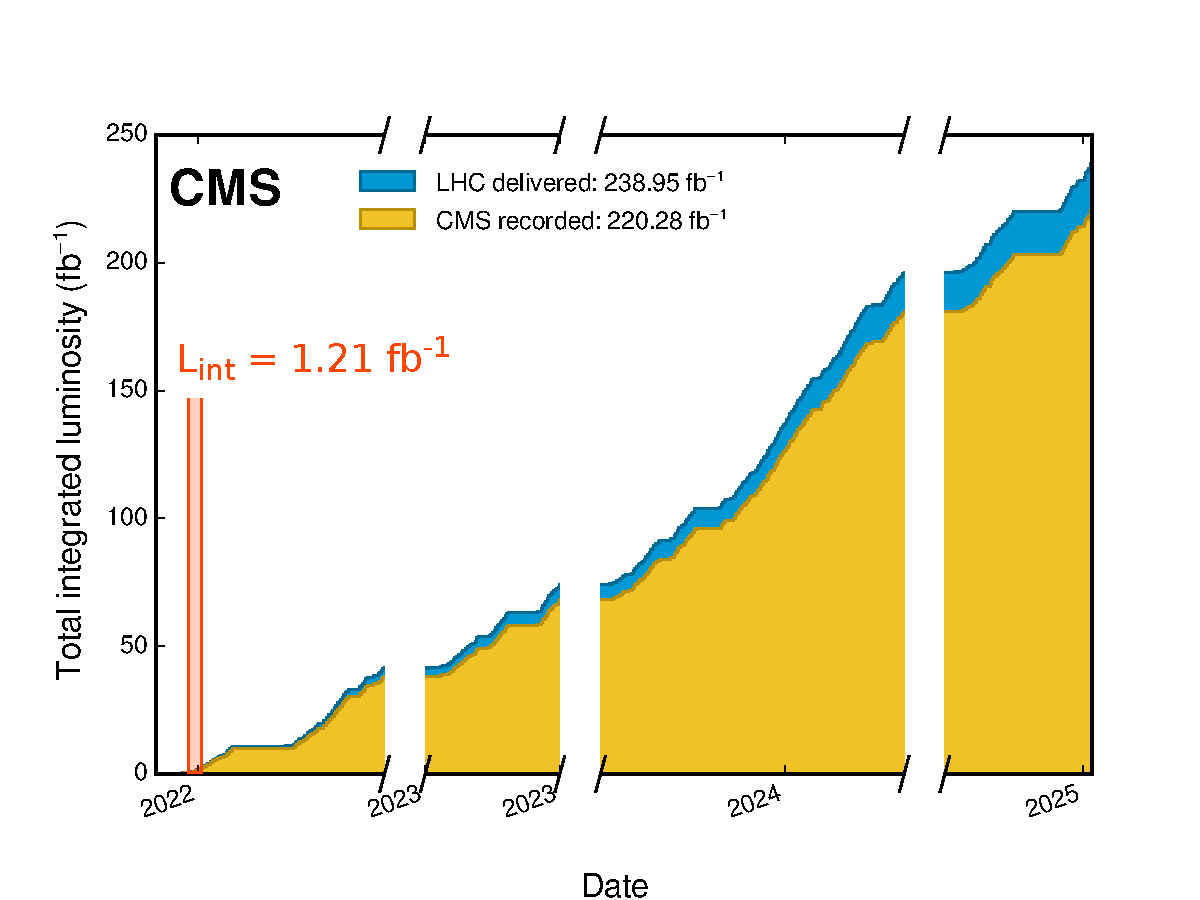
\includegraphics[width=0.8\textwidth]{figures/ttxs/lumiplot_thesis.pdf}
    \caption{\textbf{Integrated luminosity in Run~3.} The cumulative integrated luminosity delivered to and recorded by CMS in Run~3 at the time of writing, corresponding to the period July 2022--August 2025. The dataset used for the analysis in this chapter, corresponding to \lumiRIII, is marked in orange. \textit{Figure adapted from \citere{CMS:lumiplot}}.}
    \label{fig:ttxs:lumi}
\end{figure}

The results of this work were first presented as a Physics Analysis Summary in September~2022~\cite{CMS:TOP-22-012-PAS}, only two months after the start of data taking, as the first public physics result of LHC Run~3. It was published later in \textit{JHEP} as \citere{CMS:TOP-22-012}, again representing the first published Run~3 result. A similar result by ATLAS was published afterwards in \citere{ATLAS:2023slx}.

This chapter is structured as follows: In \cref{sec:ttxs:setup}, the used data sets, object definitions, and event selection criteria are described, followed by the derivation and application of needed corrections in \cref{sec:ttxs:corrections}, and the resulting data-MC agreement is shown in \cref{sec:ttxs:control}. The considered systematic uncertainties are listed in \cref{sec:ttxs:systematics}, and the fit results are presented in \cref{sec:ttxs:fitresults}. The chapter is concluded by a short summary and outlook in \cref{sec:ttxs:summary}.

\section{Data sets and event selection}
\label{sec:ttxs:setup}

In this section, the choice of data sets for experimental data and for simulation, as well as the choice of triggers, is described. Following that, the object and event selection procedure is outlined and several event categories to be used in the likelihood fit are defined. 

\subsection{Data sets}
\label{sec:ttxs:datasets}

\paragraph{Experimental data}
The measurement is performed on data recorded during the period between July 27\textsuperscript{th} and August 02\textsuperscript{nd} 2022, corresponding to an integrated luminosity of \lumiRIII. This amount of data is chosen as a balance between sensitivity and speed for the early measurement: It roughly corresponds to the point where the measurement precision is no longer primarily limited by the quantity of the data, while at the same time restricting to a data set where beam and detector conditions were stable and comparable to the data-taking in Run~2.

% TODO luminosity measurement

Both single-lepton and dilepton triggers were used to select events used in this measurement during detector operation, identifying leptons in the pseudorapidity range of $\abseta < 2.5$. The \pt requirements of the triggers are summarized in Tab.~\ref{tab:ttxs:triggers}.

\begin{table}
    \centering
    \begin{tabular}{c|c}
        Trigger & Lepton requirement \\
        \hline
        \hline
        \ejets & e($\pt > 32$ GeV) \\
        \mujets & \textmu($\pt > 27$ GeV) \\
        \ee & e($\pt > 23$ GeV) and e($\pt > 12$ GeV) \\
        \mumu & \textmu($\pt > 17$ GeV) and \textmu($\pt > 8$ GeV) \\
        \emu & e($\pt > 23$ GeV) and \textmu($\pt > 8$ GeV)  or \\
        & e($\pt > 12$ GeV) and \textmu($\pt > 23$ GeV)
    \end{tabular}
    \caption{\textbf{Trigger definitions} as used for the \ttbar cross section measurement. The leptons are required to be isolated and in the pseudorapidity range  $\abseta < 2.5$.}
    \label{tab:ttxs:triggers}
\end{table}

\paragraph{Simulation}
To compare the data with predictions, Monte Carlo (MC) simulation is used to simulate both the \ttbar signal as well as most important background processes, specifically single-top quark production in the $t$-channel, associated tW production, Z+jets production, W+jets production, and diboson (WW, WZ and ZZ) production. Example Feynman diagrams for these processes are shown in \cref{fig:ttxs:feynman}. The programs used for the different samples, as well as the respective orders in QCD, are collected in \cref{tab:ttxs:simulation}. For Z/W+jets production, up two four additional partons are included in the LO matrix element using the MLM merging scheme~\cite{Mangano:2006rw}.


\begin{figure}[t]
    \centering
    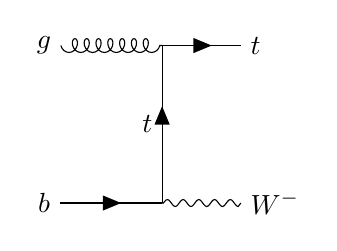
\begin{tikzpicture}[baseline=(current bounding box.center)]
      \begin{feynman}
        \vertex (i1) {\(g\)};
        \vertex [below=2.0 cm of i1] (i2) {\(b\)};
        \vertex [right=1.5 cm of i1] (a);
        \vertex [right=1.5 cm of i2] (b);
        \vertex [right=1.0 cm of a] (f1) {\(t\)};
        \vertex [right=1.0 cm of b] (f2) {\(W^-\)};
        \diagram* {
          (i1) -- [gluon] (a),
          (i2) -- [fermion] (b),
          (a) -- [anti fermion, edge label'=\(t\)] (b),
          (a) -- [fermion] (f1),
          (b) -- [boson] (f2),
        };
      \end{feynman}
    \end{tikzpicture}
    \hspace{1.0cm}
    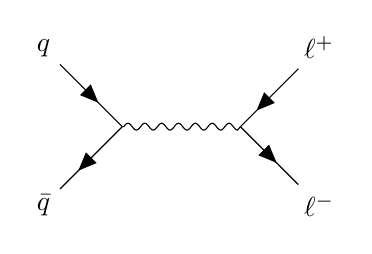
\begin{tikzpicture}[baseline=(current bounding box.center)]
      \begin{feynman}
        \vertex (i1) {\(q\)};
        \vertex [below=2.0 cm of i1] (i2) {\(\bar{q}\)};
        \vertex [below right=1.0 cm and 1.0 cm of i1] (a);
        \vertex [right=1.5 cm of a] (b);
        \vertex [right=3.5 cm of i1] (f1) {\(\ell^+\)};
        \vertex [right=3.5 cm of i2] (f2) {\(\ell^-\)};
        \diagram* {
          (i1) -- [fermion] (a),
          (i2) -- [anti fermion] (a),
          (a) -- [boson, edge label'=\(\Zgamma\)] (b),
          (b) -- [anti fermion] (f1),
          (b) -- [fermion] (f2),
        };
      \end{feynman}
    \end{tikzpicture}
    \hspace{1.0cm}
    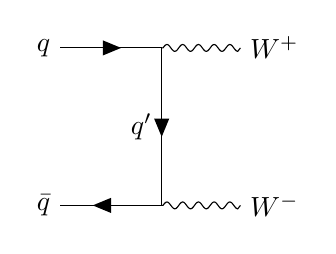
\begin{tikzpicture}[baseline=(current bounding box.center)]
      \begin{feynman}
        \vertex (i1) {\(q\)};
        \vertex [below=2.0 cm of i1] (i2) {\(\bar{q}\)};
        \vertex [right=1.5 cm of i1] (a);
        \vertex [right=1.5 cm of i2] (b);
        \vertex [right=1.0 cm of a] (f1) {\(W^+\)};
        \vertex [right=1.0 cm of b] (f2) {\(W^-\)};
        \diagram* {
          (i1) -- [fermion] (a),
          (i2) -- [anti fermion] (b),
          (a) -- [fermion, edge label'=\(q^\prime\)] (b),
          (a) -- [boson] (f1),
          (b) -- [boson] (f2),
        };
      \end{feynman}
    \end{tikzpicture} \\
    \vspace{0.3cm}
    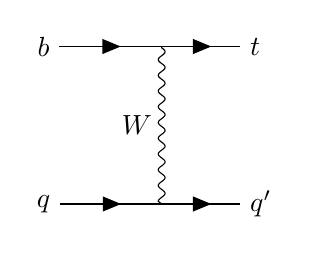
\begin{tikzpicture}[baseline=(current bounding box.center)]
      \begin{feynman}
        \vertex (i1) {\(b\)};
        \vertex [below=2.0 cm of i1] (i2) {\(q\)};
        \vertex [right=1.5 cm of i1] (a);
        \vertex [right=1.5 cm of i2] (b);
        \vertex [right=1.0 cm of a] (f1) {\(t\)};
        \vertex [right=1.0 cm of b] (f2) {\(q^\prime\)};
        \diagram* {
          (i1) -- [fermion] (a),
          (i2) -- [fermion] (b),
          (a) -- [boson, edge label'=\(W\)] (b),
          (a) -- [fermion] (f1),
          (b) -- [fermion] (f2),
        };
      \end{feynman}
    \end{tikzpicture}
    \hspace{1.0cm}
    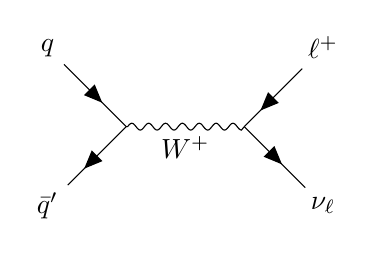
\begin{tikzpicture}[baseline=(current bounding box.center)]
      \begin{feynman}
        \vertex (i1) {\(q\)};
        \vertex [below=2.0 cm of i1] (i2) {\(\bar{q}^\prime\)};
        \vertex [below right=1.0 cm and 1.0 cm of i1] (a);
        \vertex [right=1.5 cm of a] (b);
        \vertex [right=3.5 cm of i1] (f1) {\(\ell^+\)};
        \vertex [right=3.5 cm of i2] (f2) {\(\nu_\ell\)};
        \diagram* {
          (i1) -- [fermion] (a),
          (i2) -- [anti fermion] (a),
          (a) -- [boson, edge label'=\(W^+\)] (b),
          (b) -- [anti fermion] (f1),
          (b) -- [fermion] (f2),
        };
      \end{feynman}
    \end{tikzpicture}
    \caption{\textbf{Feynman diagrams for the background processes.} Examples of Feynman diagrams for (from top left to bottom right) tW production, $\Zgamma \rightarrow \ell\ell$ production, WW production, $t$-channel single top production, and $\mathrm{W} \rightarrow \ell\nu$ production, constituting the most important backgrounds.}
    \label{fig:ttxs:feynman}
\end{figure}

All of the generated events are interfaced to \textsc{Pythia 8} for parton showering and hadronization, and further processed in a full simulation of the CMS detector as described in \cref{ch:mc}. The proton structure in the matrix element calculation is described by the NNPDF3.1 parton distribution function (PDF) set at NNLO. Note that another background contribution, from QCD-produced multijet events with fake or non-prompt leptons, is not simulated, but estimated from data (see \cref{sec:ttxs:datadriven}).

Theoretical predictions, as well as the measured integrated luminosity, are used to normalize the cross sections of the signal and background samples, which are collected in \cref{tab:ttxs:crosssections}. In particular, the \ttbar signal is normalized to a cross section of \xsecpred computed at NNLO+NNLL in QCD~\cite{Czakon:2011xx}, which is also used as a prediction for comparison with the SM.

\subsection{Object definition}
\label{sec:ttxs:objects}

\paragraph{Leptons}

Electrons or muons are considered for the analysis if they have $\pt > 10$ GeV and $\abseta < 2.4$. For electrons, the range $1.44 < |\eta_{\mathrm{SC}}| < 1.57$ is removed, where $\eta_{\mathrm{SC}}$ is the pseudorapidity of the ECAL supercluster from which the electron was reconstructed and the interval corresponds to the transition region between barrel and endcaps in the ECAL. Furthermore, additional identification criteria (ID) are applied to remove non-prompt or fake (i.e. wrongly reconstructed) leptons and enrich the selection with \ttbar events.

For electrons, the ``tight'' working point of the cut-based ID described in \citere{CMS:EGM-17-001} is applied, which includes information from both the details of the electromagnetic shower in the ECAL and the track, as well as the matching between the two. It also includes a requirement for the electron to be isolated from other particles such as hadrons, which is implemented in the form of the relative isolation variable \Irel. It is defined as the scalar \pt sum of all particles in a cone around the lepton in question, divided by the lepton \pt. Here, $\Delta R = \sqrt{(\Delta \eta)^2 + (\Delta \varphi)^2} < 0.3$ is used for the radius of the cone. Additional corrections accounting for pileup particles are applied.

\begin{table}[!t]
    \centering\renewcommand\arraystretch{1.2}
    \begin{tabular}{c|c|c}
     Process & QCD order & ME Generator \\
     \hline
     \hline
     \ttbar & NLO & \powhegvtwo (\texttt{hvq}) \\
     tW & NLO & \powhegvtwo (\texttt{ST\_wtch}) \\
     $t$-channel single top & NLO & \powhegvtwo (\texttt{ST\_tch}) + \textsc{MadSpin} \\
     Z/W+jets & LO & \amcatnlo (MLM merging)\\
     WW, WZ \& ZZ & LO & \pythia 8.2
\end{tabular}
\caption{\textbf{Simulated signal and background samples.} An overview of the different simulated processes, as well as the theoretical order in QCD and the ME generator used to simulate them. For all samples, \textsc{Pythia 8.2} is used for showering and hadronization.}
\label{tab:ttxs:simulation}
\end{table}

\begin{table}[h]
    \centering\renewcommand\arraystretch{1.2}
    \begin{tabular}{c|c|c|c}
         Process & Cross section (pb) & Order & Program / reference \\
         \hline
         \hline
         \ttbar & 921 & NNLO+NNLL & Top++~\cite{Czakon:2011xx} \\
         tW & 87.6 & NNLO (approx.) & \cite{Kidonakis:2021vob} \\
         $t$-channel single top & 232.2 & NNLO & MCFM~\cite{Campbell:2020fhf} \\
         $\Zgamma\mathrm{+jets} \rightarrow \ell\ell$ & \multirowcell{2}{$25.5 \times 10^3$} & \multirowcell{2}{NNLO} & \multirowcell{2}{DYTurbo~\cite{Camarda:2019zyx}}  \\
         $\mll > \SI{10}{\GeV}$ & & & \\
         $\mathrm{W+jets} \rightarrow \ell\nu$, & $63.2 \times 10^3$ & NNLO & DYTurbo~\cite{Camarda:2019zyx} \\
         WW & 116.8 & NNLO & MATRIX~\cite{Grazzini:2017mhc} \\
         WZ & 54.3 & NLO & MATRIX~\cite{Grazzini:2017mhc} \\
         ZZ & 16.7 & NLO & MATRIX~\cite{Grazzini:2017mhc}
    \end{tabular}
    \caption{\textbf{Cross sections for signal and background processes at \sqrtsRIII.} The cross sections used for the normalization of the signal and background processes, as well as the orders in QCD at which they were computed. Where applicable, cross sections are given as the sum of the process and its charge conjugate.}
    \label{tab:ttxs:crosssections}
\end{table}

For muons, a similar cut-based ID is used as described in \citere{CMS:MUO-16-001}, also at the tight working point. Here, criteria on the compatibility of tracks in the inner tracker, the muon detectors and the reconstructed primary vertex are employed. Again, a cut on \Irel is used, defined equivalently but with a cone size of $\Delta R < 0.4$.

\paragraph{Jets}

The anti-$k_T$ algorithm~\cite{Cacciari:2008gp} is used to cluster reconstructed particles into jets with a distance parameter of 0.4. In order for a jet to be considered, it is required to have $\pt > 30$ GeV and $\abseta < 2.4$, and jets overlapping with any considered leptons (i.e. fulfilling the above criteria) are removed. %Again, additional ID criteria, based on the fractions of \pt originating from neutral hadron, charged hadron and electromagnetic jet constituents, are used to reject 

\paragraph{Tagging of b jets}

A special role is played by jets originating from the showering and hadronization of b quarks. Naively, two such jets are expected per \ttbar event from the two top decays, although in practice one or both jets may fall out of acceptance of the detector or otherwise not be identified. Furthermore, additional b quarks may be produced by radiation at higher orders in QCD. Correctly tagging these jets as such can greatly improve signal purity by cutting away backgrounds such as Z+jets, W+jets and QCD multijet events.

Here, the \textsc{DeepJet} algorithm~\cite{DeepJet:2020,CMS:BTV-16-002}, which is based on a deep neural network (DNN) classifier, is used to identify (``tag'') b jets. A working point with an identification efficiency of more then 75\% is used, with misidentification rates of around 17\% for charm jets and around 1\% for other jets from light quarks or gluons.

\subsection{Channel definition}
\label{sec:ttxs:channels}

Events are selected with either one or two leptons, corresponding respectively to the \ljets and dilepton decay channels of \ttbar. They are categorized into separate channels by their lepton flavor content, and additional requirements are applied for the different channels. 

\paragraph{Dilepton channels}

Events with exactly two leptons, required to have opposite electric charge, are sorted into three dilepton channels (\emu, \ee, and \mumu). The presence of at least one jet is required, and in the same-flavor channels (\ee and \mumu), at least one jet is required to be b tagged in order to reject Z+jets and QCD multijet background. In the much purer \emu channel, on the other hand, events without b tags are retained to later help constrain the b tagging efficiency in the fit to data.

In order to reject even more Z+jets background, events in the same-flavor channels with an invariant dilepton mass of $| \mll - m_Z | < 15$ GeV, where $m_Z$ is the Z boson mass, are removed.

\paragraph{\ljets channels}

Events with exactly one lepton are sorted into the \ejets or \mujets channels based on their flavor. At least three jets are required, of which at least one needs to be b tagged. Note that regardless of these selections, there is still non-negligible background from QCD multijet events where the lepton is non-prompt or fake, which is estimated from data (see \cref{sec:ttxs:datadriven}).

\paragraph{\pt requirement}

In all channels, the considered leptons are required to have $\pt > 35$ GeV. This requirement is needed in the \ljets channels in order to stay above the single-lepton trigger \pt thresholds (compare Tab. \ref{tab:ttxs:triggers}). In this measurement, the choice is made to apply the same \pt requirement also both leptons in the dilepton channels to ensure consistency between the lepton definitions. This is done to help constrain the lepton ID scale factors using the combination of lepton flavor channels, which otherwise might not be accurate since the scale factors for different lepton definitions might differ. In particular it opens up the possibility to extract a result on the cross section without any prior knowledge on the lepton ID efficiencies, which was done in the first published version of this analysis \cite{CMS:TOP-22-012-PAS}. %\todo{decide on whether to add this cross check here}% and is included in this thesis as a cross-check (see sec. ??).

\paragraph{b tag and jet categorization}

In practice, the efficiency of the b tagging algorithm used might be different between simulation and data, necessitating a correction to prevent bias. In this analysis, this efficiency is measured simultaneously with the cross section directly in the data. To do so, the lepton flavor channels are additionally split into categories based on the number (exactly 0, 1, or 2) of b tagged jets. Since only the \emu channel allows events with 0 b tags, this results in 11 categories total. To gain further sensitivity to the b tagging efficiency and to increase possible separation between \ttbar signal and background, the selected events are finally coarsely binned into the number of accepted jets for the eventual fit, giving a total number of 40 bins.


\section{Corrections}
\label{sec:ttxs:corrections}

While the simulation used in CMS tries to describe as many physics and detector effects as possible, in practice it should always be expected that not all observables agree with the experimental data perfectly. This is especially true for an early analysis such as this, as the detector conditions might have changed significantly during the long shutdown between LHC Runs 2 and 3, and the simulation had not been recalibrated at the time of the measurement. 

Because of this, the analysis setup is designed to either directly measure or cross-check as many required experimental calibration and correction factors as possible. This includes pileup corrections, efficiency scale factors for triggers, electrons, muons and b tags, as well as jet energy corrections, all of which are briefly described in this section.

In addition to these experimental corrections, background processes might also be imperfectly described by the simulation because of theoretical shortcomings. In this case, ways have to be found to correct them directly from the experimental data. Here, two such cases are relevant and will be presented in the latter half of this section: The Z+jets background in the dilepton channels and in the presence of b tagged jets, for which the normalization is taken from data; and the QCD background in the \ljets channels, which uses a fully data-driven estimation and foregoes simulation entirely.

\subsection{Experimental corrections}
\label{sec:ttxs:scalefactors}

\paragraph{Pileup reweighting}

The simulation samples used in this analysis were generated before the start of Run 3 data taking using a projected estimate of the average pileup. As a result, the pileup distribution in the simulation does not match the one observed in data, which could influence mostly jet-related variables such as the number of jets and the jet \pt.

Since at the time of the measurement, no theory-based calculation for the correct pileup distribution were available, an experimental approach was taken. Three experimental observables that are strongly correlated with pileup were identified: 

\begin{itemize}
    \item The number of well-reconstructed primary vertices per event $n_{\mathrm{PV}}$;
    \item The median \pt density in the calorimeter, calculated from calorimeter-only jets as $\rho^{\mathrm{calo}} = \mathrm{med} (\pt / A)$, where $A$ is the jet area defined in the $\varphi$-$\eta$ plane and the median is taken over all jets in the event;
    \item The median \pt density in the tracker $\rho^{\mathrm{trk}}$, defined equivalently as $\rho^{\mathrm{calo}}$, but for jets calculated only from tracker information.
\end{itemize}

A binned reweighting from simulation to data is derived for each observable based on the full data sample, and the average of the three weights is applied to the simulation, so that approximate agreement is achieved in all three variables. The distributions before and after reweighting can be seen in \cref{fig:ttxs:pileup}.

% outputs/2022_datamc_run3jec_nopileup_300822
% outputs/2022_datamc_ul18jec_pu_triggersf_310822

\begin{figure}[p]
    \centering
    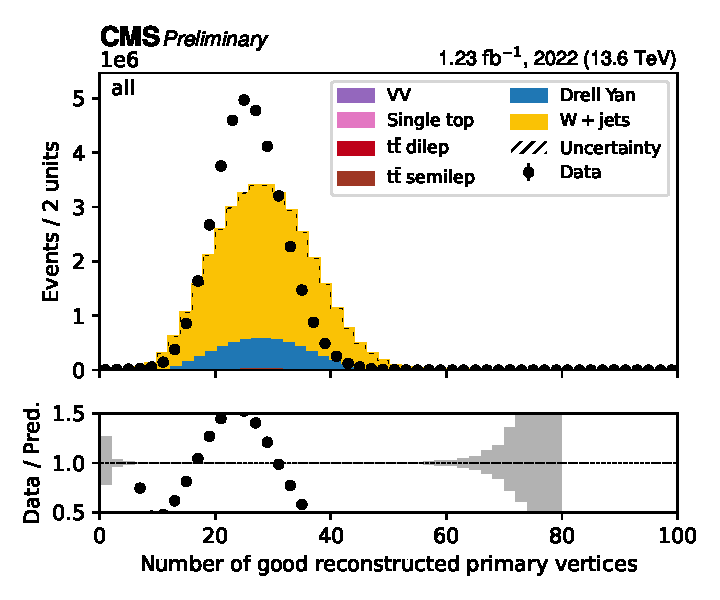
\includegraphics[width=0.49 \textwidth]{figures/ttxs/pileup/nvtx_orig.pdf}
    \hfill
    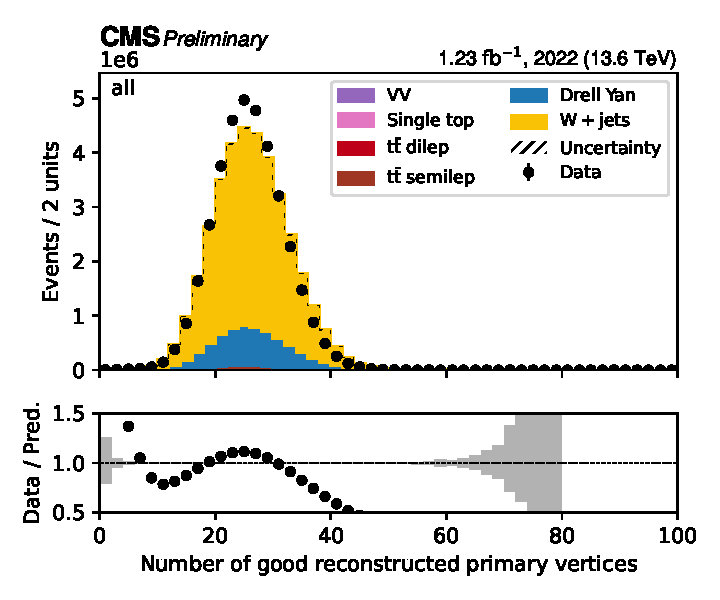
\includegraphics[width=0.49 \textwidth]{figures/ttxs/pileup/nvtx_reweighted.pdf}
    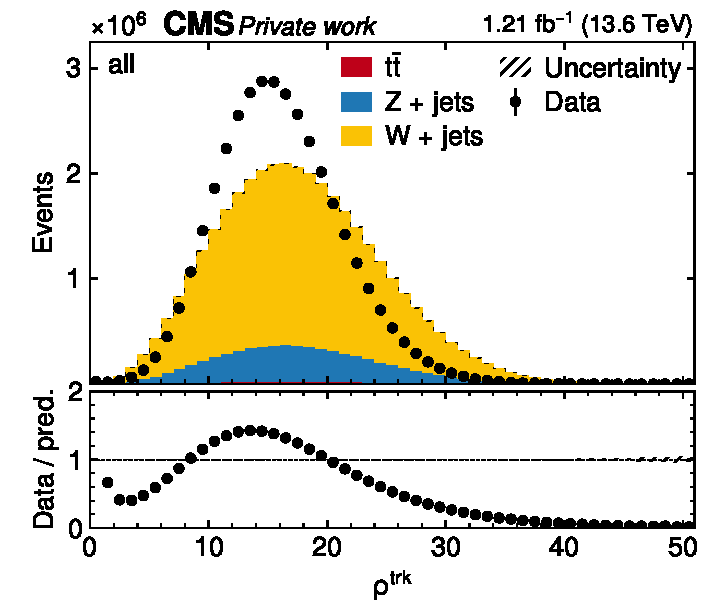
\includegraphics[width=0.49 \textwidth]{figures/ttxs/pileup/rhoFastjetCentralChargedPileUp_orig.pdf}
    \hfill
    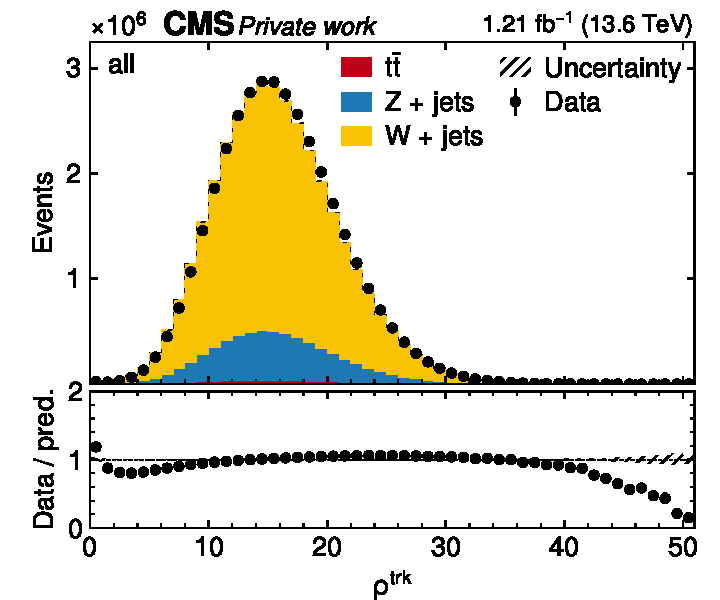
\includegraphics[width=0.49 \textwidth]{figures/ttxs/pileup/rhoFastjetCentralChargedPileUp_reweighted.pdf}
    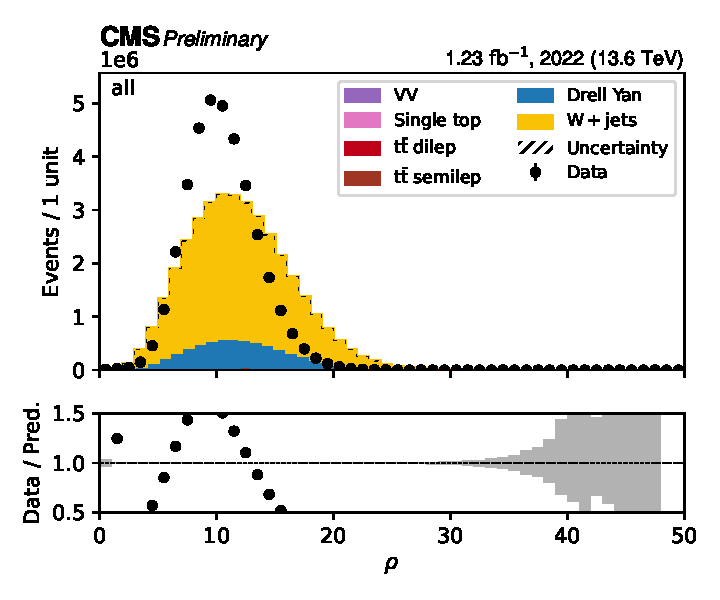
\includegraphics[width=0.49 \textwidth]{figures/ttxs/pileup/rhoFastjetCentralCalo_orig.pdf}
    \hfill
    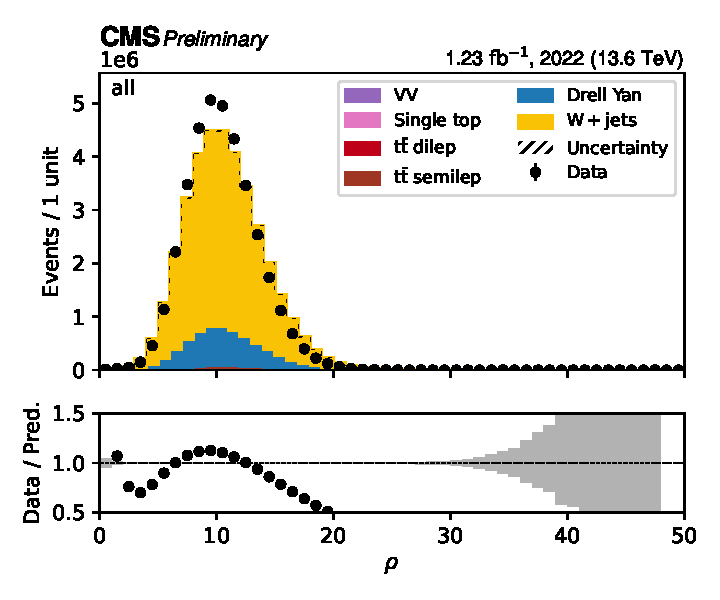
\includegraphics[width=0.49 \textwidth]{figures/ttxs/pileup/rhoFastjetCentralCalo_reweighted.pdf}
    \caption{\textbf{Pileup reweighting.} Pileup-related distributions in MC and data in before (left) and after reweighting (right). From top to bottom: number of primary vertices as well as the mean energy densities $\rho^{\mathrm{trk}}$ (calculated using tracker input) and $\rho^{\mathrm{calo}}$ (calculated using calorimeter input).}
    \label{fig:ttxs:pileup}
  \end{figure}

\paragraph{Trigger scale factors}

The trigger efficiency, i.e. the probability for an event falling into the selection phase space to be triggered by the low- and high-level triggers, can differ between simulation and data.
In principle, both dilepton and single-lepton triggers are used for this measurement and should be considered for the efficiency calculation. However, due to the high offline \pt requirements for the two leptons applied in all channels, the fraction of events that are triggered only by the dilepton triggers is negligibly small, and can be neglected for the purpose of determining the scale factor. Thus, only the single-lepton triggers are considered in this section for simplicity.
%It should be noted that, while both dilepton and single-lepton triggers are used for the measurement, the single-lepton triggers by far dominate the selected event count due to the high \pt thresholds required, and so the efficiency is measured for the single-lepton triggers only for simplicity.

The efficiency measurement is performed by the so-called tag-and-probe (T\&P) method, using $\mathrm{Z} \rightarrow \mathrm{e^+ e^-}$ and $\mathrm{Z} \rightarrow \mathrm{\mu^+ \mu^-}$ events. They are selected using the same definitions presented above, including the lepton identification, except for requiring their invariant mass to fulfill $| \mll - m_Z | < 20$ GeV. At least one of the leptons is required to pass the relevant single-lepton trigger and is then designated the tag, while the other lepton might or might not pass the trigger and is designated the probe. Assuming the probability for the two leptons to pass the trigger to be independent of each other, the trigger efficiency, given by probability of the probe to pass, can be written as

\begin{equation}
    \epsilon_{\mathrm{tr}} = \frac{N (\text{Probe passes})}{ N (\text{Probe passes}) + \frac{1}{2} N (\text{Probe fails}) }
\end{equation}

where $N$ corresponds to to the number of events in which the second lepton either passes or fails the trigger, and the combinatoric factor $\frac{1}{2}$ comes from the fact that either one or the other lepton can fail. 

The efficiency is measured in this way in coarse bins of lepton \pt and \abseta, separately for muons and electrons, in both simulation and experimental data. It is then applied to simulation in the following way: For \ljets events, a simple ratio $\epsilon_{\mathrm{tr,data}} / \epsilon_{\mathrm{tr,sim}}$ is applied to each simulation event as a scale factor, which is displayed in \cref{fig:ttxs:triggersf}. For dilepton events, on the other hand, the fact that only one lepton needs to pass the single-lepton trigger needs to be taken into account. This leads to a per-event efficiency given by

\begin{equation}
\label{eq:ttxs:triggersf}
    \epsilon_{\mathrm{tr,\ell \ell}} = \epsilon_{\mathrm{tr,\ell 1}} + \epsilon_{\mathrm{tr,\ell 2}} - \epsilon_{\mathrm{tr,\ell 1}} \epsilon_{\mathrm{tr,\ell 2}}
\end{equation}

where $\epsilon_{\mathrm{tr,\ell 1}}$ and $\epsilon_{\mathrm{tr,\ell 2}}$ are the efficiencies evaluated at the \pt and \abseta of the two leptons, respectively. Again, the ratio of this event efficiency in data and simulation is applied to the simulation.

\begin{figure}[t]
    \centering
    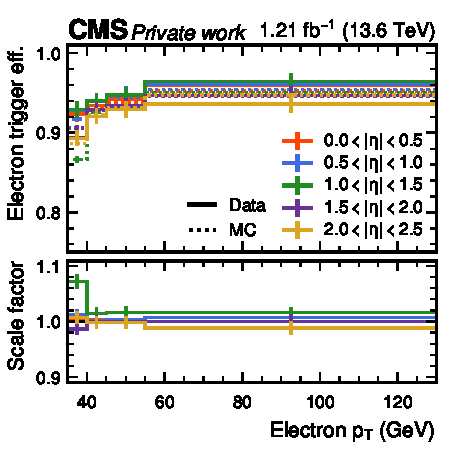
\includegraphics[width=0.49 \textwidth]{figures/ttxs/scalefactors/trigger_eff_e.pdf}
    \hfill
    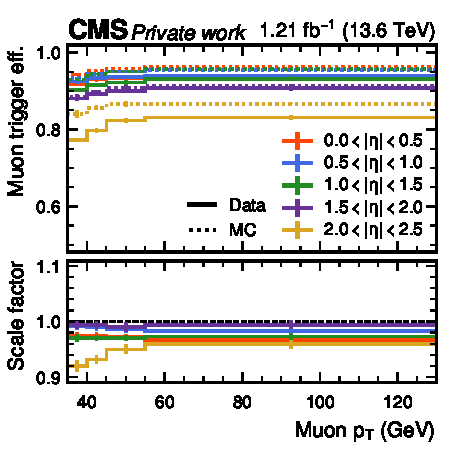
\includegraphics[width=0.49 \textwidth]{figures/ttxs/scalefactors/trigger_eff_mu.pdf}
    \caption{\textbf{Trigger scale factors.} Single-lepton trigger efficiencies in data and MC (top) and scale factors (bottom) for electrons (left) and muons (right) as a function of lepton \pt and $|\eta|$, calculated using a tag-and-probe-method. The error bars designate both statistical and systematic uncertainties.}
    \label{fig:ttxs:triggersf}
\end{figure}

\paragraph{Lepton scale factors}

Similarly to the triggers, the reconstruction and identification of leptons can exhibit different efficiencies between simulation and data, and thus require scale factors. 
%Two orthogonal approaches are taken with respect to this: In the first approach, 
The efficiencies are measured with a similar tag-and-probe method as for the triggers, and the simulation is corrected to the data. This is the standard approach commonly taken in CMS, detailed in \citeres{CMS:EGM-17-001,CMS:MUO-16-001} for electrons and muons, respectively.%, and will be used in the figures presented in this thesis unless stated otherwise. 
The efficiency measurement was not performed as part of this thesis, but is still shown in \cref{fig:ttxs:muonsf,fig:ttxs:elesf} for reference. The muon scale factors are split into a reconstruction and an identification part, while these are combined for the electron scale factors.  

\begin{figure}[t]
    \centering
    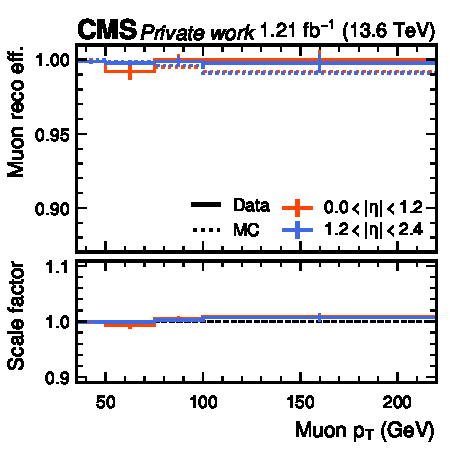
\includegraphics[width=0.49 \textwidth]{figures/ttxs/scalefactors/lepton_eff_mu_reco.pdf}
    \hfill
    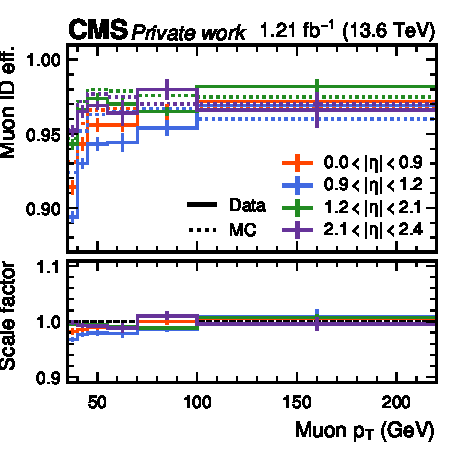
\includegraphics[width=0.49 \textwidth]{figures/ttxs/scalefactors/lepton_eff_mu_id.pdf}
    \caption{\textbf{Muon scale factors}. Muon efficiencies in data and MC (top) and scale factors (bottom), split into reconstruction (left) and identification (right) and shown as a function of lepton \pt and $|\eta|$, calculated using a tag-and-probe-method. The error bars designate both statistical and systematic uncertainties.}
    \label{fig:ttxs:muonsf}
  \end{figure}
  
  \begin{figure}[t]
    \centering
    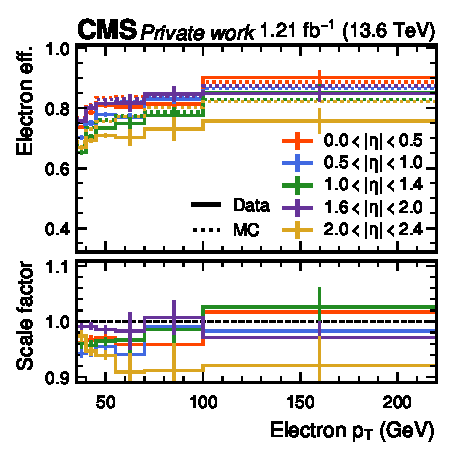
\includegraphics[width=0.49 \textwidth]{figures/ttxs/scalefactors/lepton_eff_e.pdf}
    \caption{\textbf{Electron scale factors.} Combined electron efficiencies in data and MC (top) and scale factors (bottom) as a function of lepton \pt and $|\eta|$, calculated using a tag-and-probe-method. The error bars designate both statistical and systematic uncertainties.}
    \label{fig:ttxs:elesf}
  \end{figure}

%In the second, alternative, approach, on the other hand, no correction to the simulation is made, and instead the lepton efficiencies in data in the selection phase space are measured simultaneously with the cross section using the likelihood fit. This will be further described in sec. ??.

\paragraph{b tagging scale factors}

The performance of b tagging algorithms, such as the \textsc{DeepJet} algorithm used in this analysis, is known to differ between simulation and data, necessitating corrections. This is particularly relevant here, as the multivariate classifier behind \textsc{DeepJet} had not been re-trained on Run~3 data at the time of the measurement; instead, the Run~2 calibration was used. 

Since no external calibration of b tagging efficiencies for Run~3 was available within the timeframe of this study, the b tagging efficiency in data is extracted directly from the data itself. This is achieved by performing a simultaneous likelihood fit with the ttbar cross section, as described in \cref{sec:ttxs:systematics}. As a result, no b tagging scale factors are applied beforehand. 

\paragraph{Jet energy corrections}

Another observable that often differs significantly between observed data and simulation is the measured energy response of the jets. Both its mean value, the jet energy scale (JES), and the jet energy resolution (JER) require corrections, which are together referred as jet energy corrections (JECs). Both are centrally provided by CMS following the methods of \citere{CMS:JME-13-004}. 

The derivation of the JES is performed in multiple steps:
first, the expected fraction of jet energy due to pileup, determined from MC simulation, is removed from all jets in data and MC. Second, the difference in jet energy between detector- and particle-level jets in simulation is determined as a function of jet kinematics, and detector-level jets are corrected accordingly in both data and simulation.
Third, residual disagreements of the simulation with the data are corrected using experimental jet measurements in dijet, $\gamma$+jets, Z+jets, and multijet events, again parametrized as a function of jet kinematics~\cite{CMS:JME-13-004}.

Similarly, JER scale factors are determined by correcting the resolution in simulation to the one seen in data, based on dijet, $\gamma$+jets and Z+jets events~\cite{CMS:JME-10-011}. They are then applied to jets in simulation by scaling the difference between detector- and particle-level jet energy for jets where a matched particle-level jet is found, while a stochastic smearing is used otherwise.


\subsection{Data-driven background estimation}
\label{sec:ttxs:datadriven}

\paragraph{QCD background}

A significant background contribution in the \ljets channels, especially in the categories with only one b tag, is given by QCD multijet events with one reconstructed lepton. The lepton in question might be non-prompt, e.g. from radiated photons splitting into leptons or decays of heavy flavor hadrons, or it might be fake, i.e. a different particle (such as a photon or pion in the case of electrons) misidentified as a lepton.

It is often not practical to estimate this background using MC simulation as is done for the other backgrounds in this analysis. The reason is that, due to the large cross section of QCD multijet events at the LHC but low ratio of events with a fake or non-prompt lepton, very large MC data sets are needed to achieve significant statistics in the selected phase space, requiring excessive computing power. In addition to that, fake leptons are known not to be well-described by the simulation.

Instead, a fully data-driven approach is taken to estimate the QCD background in the \ljets channels. For this, multiple control regions (CRs) orthogonal to the signal region (SR) are defined. In the first CR, denoted ``QCD CR'', the same cuts as in the SR are applied, except that the requirement for the single lepton to be isolated from other particles (\Irel, see \cref{sec:ttxs:objects}) is inverted. It is expected that QCD events that fall in either the QCD CR or the SR show similar shapes in observable distributions, as long as said observables are uncorrelated with the lepton isolation. Thus, the shape of the QCD background can be extracted from the CR and applied in the SR. \cref{fig:ttxs:np_plots_mj_CR,fig:ttxs:np_plots_ej_CR} show the distributions of several key distributions for the QCD background in the \mujets and \ejets channels, respectively, which is estimated by subtracting all simulated (MC) processes from the data.

\begin{figure}[!ht]
    \centering
    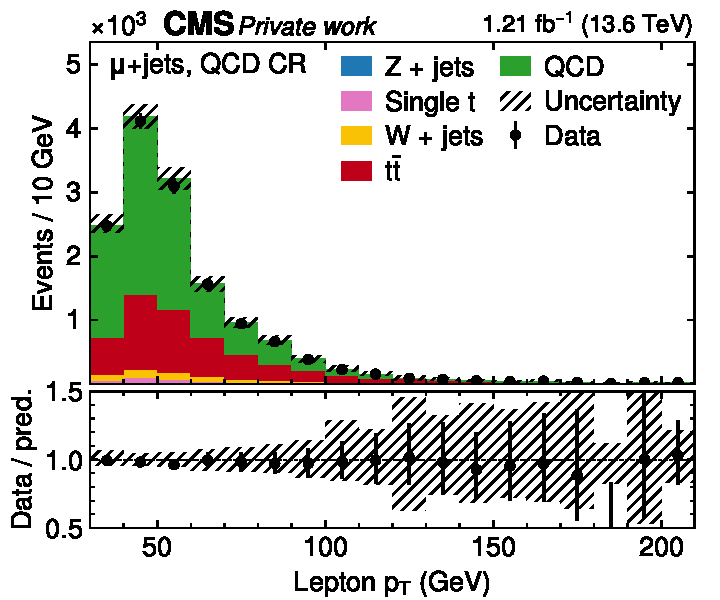
\includegraphics[width=0.49 \textwidth]{figures/ttxs/np_plots_run3/lep_pt_mj_CR.pdf}
    \hfill
    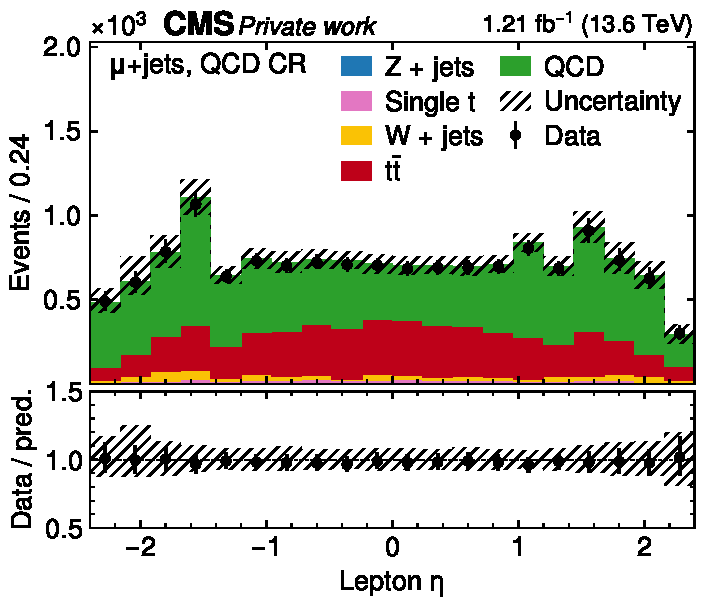
\includegraphics[width=0.49 \textwidth]{figures/ttxs/np_plots_run3/lep_eta_mj_CR.pdf}
    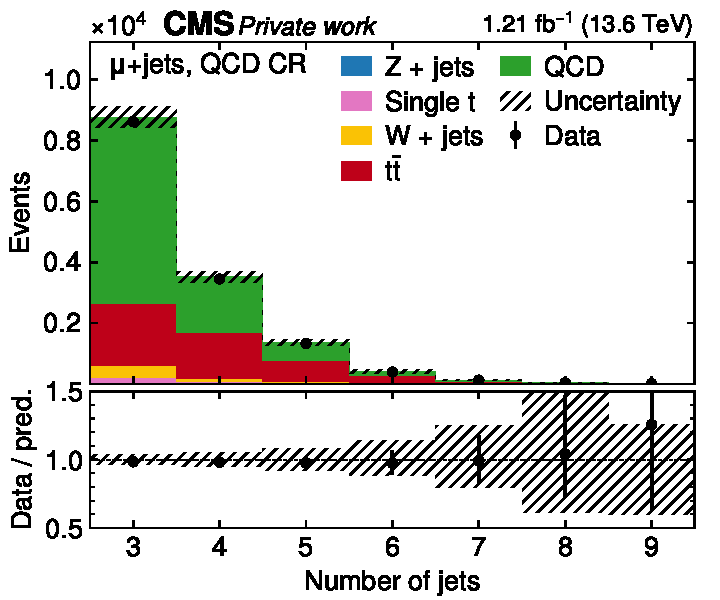
\includegraphics[width=0.49 \textwidth]{figures/ttxs/np_plots_run3/njet_mj_CR.pdf}
    \hfill
    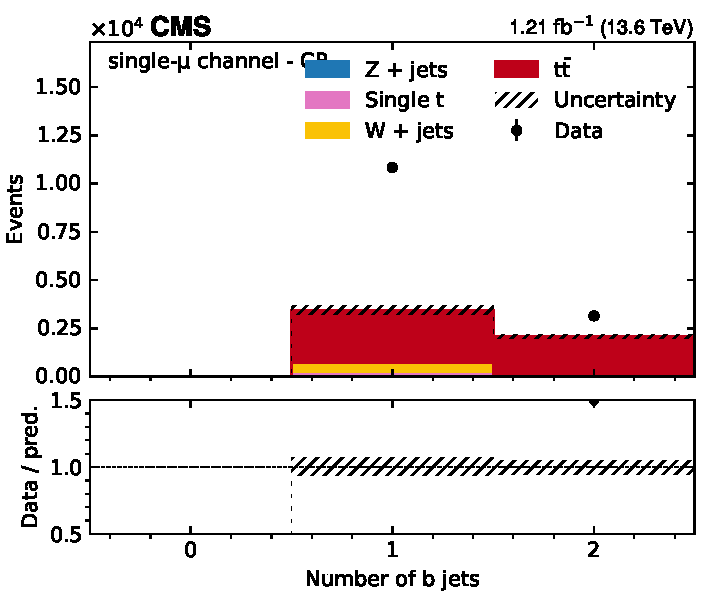
\includegraphics[width=0.49 \textwidth]{figures/ttxs/np_plots_run3/nbtag_mj_CR.pdf}
    \caption{\textbf{QCD control region for \mujets.} Distributions in the QCD CR for the \mujets channel. From top left to bottom right: $\pt$ of the lepton, $\eta$ of the lepton, the number of jets, and the number of b-tagged jets. The uncertainty bands include MC statistical and systematic uncertainties. The difference between data and MC prediction is considered QCD background and shown in green.}
    \label{fig:ttxs:np_plots_mj_CR}
\end{figure}

\begin{figure}[!ht]
    \centering
    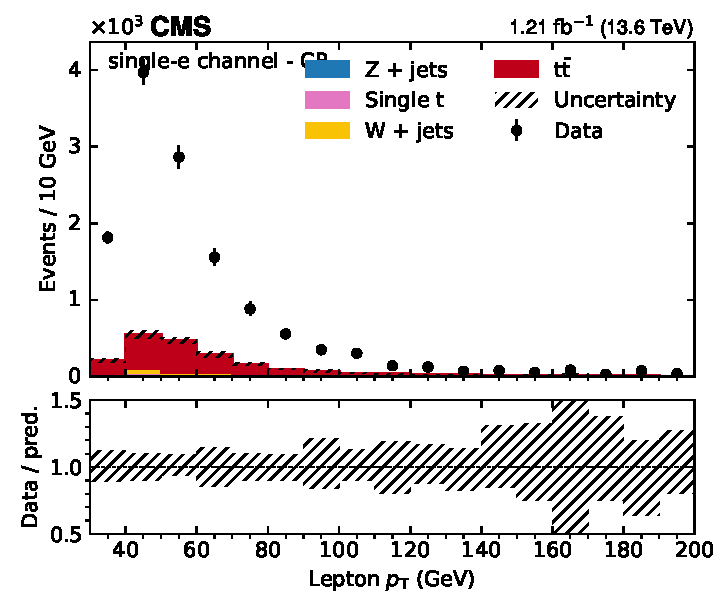
\includegraphics[width=0.49 \textwidth]{figures/ttxs/np_plots_run3/lep_pt_ej_CR.pdf}
    \hfill
    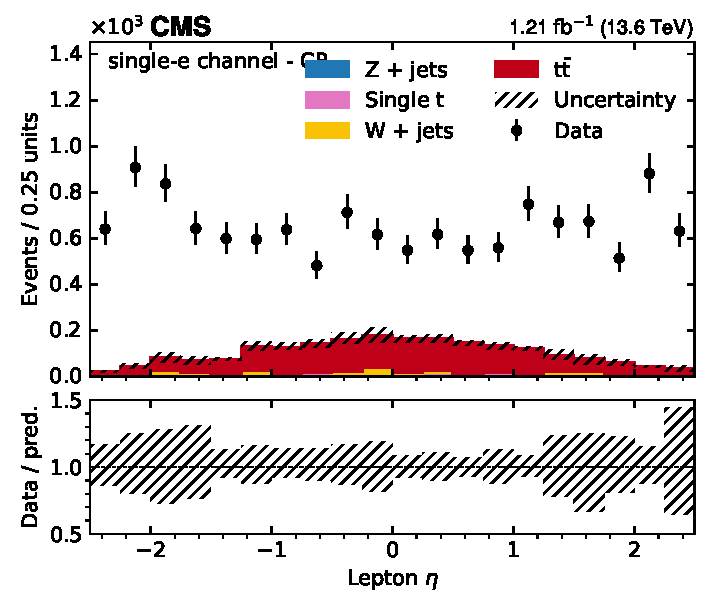
\includegraphics[width=0.49 \textwidth]{figures/ttxs/np_plots_run3/lep_eta_ej_CR.pdf}
    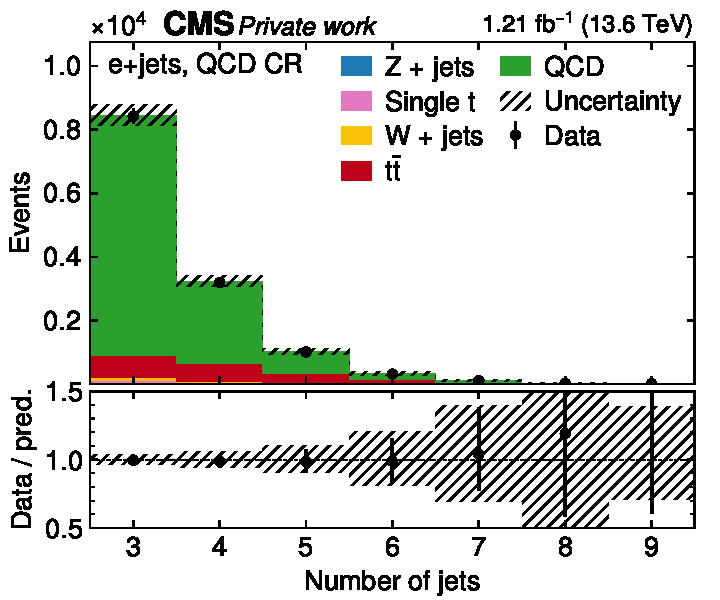
\includegraphics[width=0.49 \textwidth]{figures/ttxs/np_plots_run3/njet_ej_CR.pdf}
    \hfill
    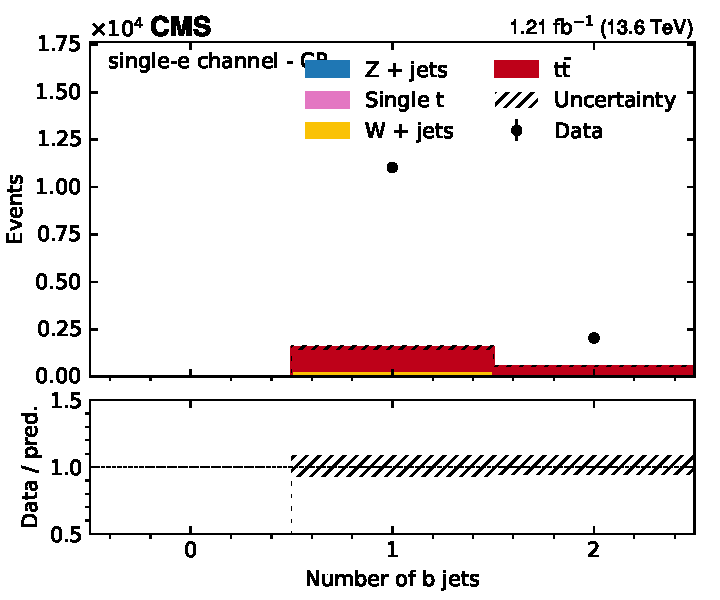
\includegraphics[width=0.49 \textwidth]{figures/ttxs/np_plots_run3/nbtag_ej_CR.pdf}
    \caption{\textbf{QCD control region for \ejets.} Distributions in the QCD CR for the \ejets channel, same as in \cref{fig:ttxs:np_plots_mj_CR}. The difference between data and MC prediction is considered QCD background and shown in green.}
    \label{fig:ttxs:np_plots_ej_CR}
  \end{figure}

The normalization of the QCD background is fixed through the so-called \textit{ABCD method}~\cite{CDF:1995eix,CDF:2000gwd}, for which an additional CR (the ``1-jet CR'') is defined.
It again contains events that pass the main selection, except for requiring exactly one jet (as opposed to at least three jets in the SR or QCD CR). These events are enriched with QCD events and contain negligible amounts of \ttbar signal. They are used to measure the ratio $f_{\mathrm{fake}}$ of QCD events that pass or fail the lepton isolation requirement, given by

\begin{equation}
\label{eq:ttxs:abcd_fakerate}
    f_{\mathrm{fake}} = \frac{ N_{\text{1 jet, pass}}^{\text{data}} - N_{\text{1 jet, pass}}^{\text{MC}} }{ N_{\text{1 jet, fail}}^{\text{data}} - N_{\text{1 jet, fail}}^{\text{MC}} }
\end{equation}

\noindent where $N_{\text{1 jet, pass}}$ and $N_{\text{1 jet, fail}}$ denote 1-jet-events that pass and fail the lepton isolation requirement, respectively; ``data'' refers to the experimental data, and ``MC'' refers to the sum of all non-QCD processes, which are estimated by MC simulation. Here, this ratio is measured in four coarse bins of lepton \pt and \abseta to accurately model lepton-related distributions; it can be seen in \cref{fig:ttxs:fakerate}.

\begin{figure}[!ht]
    \centering
    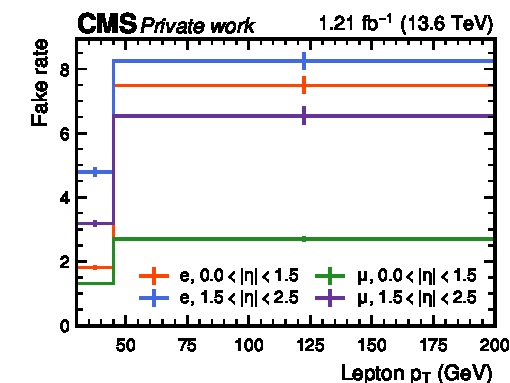
\includegraphics[width=0.58 \textwidth]{figures/ttxs/np_plots_run3/fakerate.pdf}
    \caption{\textbf{QCD fake rate}. The fake rate for the QCD background estimated in the 1 jet bin, separately for electrons and muons as, a function of lepton \pt and $|\eta|$. The error bars designate statistical uncertainties only.}
    \label{fig:ttxs:fakerate}
\end{figure}

Naively, the full distribution of the QCD background in the SR for any observable can then be written as

\begin{equation}
\label{eq:ttxs:abcd_naive}
    N_{\text{SR}}^{\text{QCD}} = ( N_{\text{CR}}^{\text{data}} - N_{\text{CR}}^{\text{MC}} ) \times f_{\mathrm{fake}}
\end{equation}

\noindent where $N_{\text{CR}}^{\text{data}}$ and $N_{\text{CR}}^{\text{MC}}$ refer to the total data and non-QCD MC yields in the QCD CR.

In practice, this is complicated by the fact that a non-negligible amount of \ttbar signal is present in the QCD CR, whose cross section, as the parameter of interest in the measurement, is not known \textit{a priori}. %A modified method to correct for this is given in Appendix ??.
To circumvent this problem, a modified method is introduced, which is agnostic about the prediction for the \ttbar cross section. 
One sets for the SR

\begin{equation}
\label{eq:ttxs:abcd_modified1}
    N^{\mathrm{data}}_{\mathrm{SR}} = N^{\ttbar}_{\mathrm{SR}}+ N^{\mathrm{MC,BG}}_{\mathrm{SR}} + N^{\mathrm{QCD}}_{\mathrm{SR}}
\end{equation}

\noindent and similarly for the QCD CR

\begin{equation}
\label{eq:ttxs:abcd_modified2}
    N^{\mathrm{data}}_{\mathrm{CR}} = N^{\ttbar}_{\mathrm{CR}} + N^{\mathrm{MC,BG}}_{\mathrm{CR}} + N^{\mathrm{QCD}}_{\mathrm{CR}},
\end{equation}

\noindent where $N^{\mathrm{data}}$ is the total data yield, $N^{\ttbar}$ is the \ttbar signal contribution, $N^{\mathrm{MC,BG}}$ is the contribution of non-QCD backgrounds as predicted by MC, and $N^{\mathrm{QCD}}$ is the QCD contribution. It is assumed that the ratio $f_{\mathrm{sig}}$ of signal events in the SR and QCD CR (but not necessarily the normalization) is correctly predicted by MC:

\begin{equation}
\label{eq:ttxs:abcd_modified3}
    f_{\mathrm{sig}} := \frac{ N^{\ttbar}_{\mathrm{CR}} }{ N^{\ttbar}_{\mathrm{SR}} } = \frac{ N^{\mathrm{\ttbar,MC}}_{\mathrm{CR}} }{ N^{\mathrm{\ttbar,MC}}_{\mathrm{SR}} }
\end{equation}

Furthermore, one sets similar to \cref{eq:ttxs:abcd_naive}

\begin{equation}
\label{eq:ttxs:abcd_modified4}
    N^{\mathrm{QCD}}_{\mathrm{SR}} = N^{\mathrm{QCD}}_{\mathrm{CR}} \times f_{\mathrm{fake}}
\end{equation}

\noindent where $f_{\mathrm{fake}}$ is still given by \cref{eq:ttxs:abcd_fakerate}, which is unaffected since the \ttbar signal contamination in the 1-jet CR is negligible.

Combining all these equations, one can first replace $N^{\ttbar}_{\mathrm{CR}}$ in \cref{eq:ttxs:abcd_modified2} by $f_{\mathrm{sig}} N^{\ttbar}_{\mathrm{SR}}$ according to \cref{eq:ttxs:abcd_modified3}, then eliminate $N^{\ttbar}_{\mathrm{SR}}$ in favor of $N^{\mathrm{data}}_{\mathrm{SR}}$, i.e. the total data yield in the SR, and get

\begin{equation}
    N^{\mathrm{QCD}}_{\mathrm{SR}} = f_{\mathrm{fake}} \, \left( N^{\mathrm{data}}_{\mathrm{CR}} - N^{\mathrm{MC,BG}}_{\mathrm{CR}} - f_{\mathrm{sig}} \left( N^{\mathrm{data}}_{\mathrm{SR}} - N^{\mathrm{MC,BG}}_{\mathrm{SR}} - N^{\mathrm{QCD}}_{\mathrm{SR}} \right) \right) .
\end{equation}

Solving this equation for $N^{\mathrm{QCD}}_{\mathrm{SR}}$ finally yields the corrected QCD contribution in the SR:

\begin{equation}
\label{eq:ttxs:abcd_modified}
    N^{\mathrm{QCD}}_{\mathrm{SR}} = \left( N^{\mathrm{data}}_{\mathrm{CR}} - N^{\mathrm{MC,BG}}_{\mathrm{CR}} - f_{\mathrm{sig}} ( N^{\mathrm{data}}_{\mathrm{SR}} - N^{\mathrm{MC,BG}}_{\mathrm{SR}} )\right)
    \times \frac{ f_{\mathrm{fake}} } {1 - f_{\mathrm{sig}} f_{\mathrm{fake}}}
\end{equation}

The resulting QCD distributions from this method are further treated in the same way as the MC backgrounds, and can be seen together with them in \cref{fig:ttxs:control_em,fig:ttxs:control_eemm,fig:ttxs:control_ljets}.
  

\paragraph{Z+jets background}

In contrast to the QCD background, the Z+jets background is generally well-described by MC simulation. 
However, in the considered phase space, the requirement of at least one reconstructed b jet can introduce modeling challenges, as b quarks are treated as massless at the matrix-element level. This approximation may lead to inaccuracies in the predicted kinematic properties of b quarks compared to those observed in data.
%However, in the phase space used in the analysis, there can be problems related to the requirement of at least one reconstructed b jet. In Z+jets events, b quarks can in principle be produced as real emissions through higher-order corrections in QCD. However, in the LO simulation used here this is done by the parton shower, which might lead to poor modeling of the b quark properties compared to data. This in turn could influence the acceptance of Z+jets events, leading to an incorrect normalization in events with one or more b tags.

Here, a data-driven normalization is derived for Z+jets events with one or two b tags in the dilepton channels, following the method of \citere{CMS:EXO-22-014-PAS}. This is important especially in the same-flavor channels, where Z+jets is a dominant background.

The normalization is derived using a CR in which the cut on \mll is inverted, i.e. in events with $| \mll - m_Z | < 15$ GeV (``inside the Z window''), which are strongly enriched in Z+jets contributions. It is assumed that the Z+jets contribution in the \emu channel (which stems mostly from $\mathrm{Z} \rightarrow \tau \tau$ events) is negligible compared to the \ee and \mumu channels, and that all other backgrounds (including \ttbar) are approximately equal in the three dilepton channels up to combinatorics, in the sense that their differences are small compared to the Z+jets event yield. Then, said Z+jets yield in the Z window in the same-flavor channels can be estimated directly from data by subtracting the \emu channel -- and with it, the other backgrounds - from the \ee and \mumu channels. This results in

\begin{equation}
\label{eq:ttxs:zjets_yield}
    N_{\mathrm{ee / \mu\mu}}^{\mathrm{Z+jets}} = N_{\mathrm{ee / \mu\mu,\,in}}^{\mathrm{data}} - \frac{1}{2} N_{\mathrm{\emu,\,in}}^{\mathrm{data}} \, k_{\mathrm{ee / \mu\mu,\,in}}
\end{equation}

\noindent where $N_{\mathrm{\ell \ell},\,in}^{\mathrm{data}}$ refers to the number of observed events inside the Z window for the respective channel, and $k_{\mathrm{ee}} = k_{\mathrm{\mu\mu}}^{-1} = \sqrt{N_{\mathrm{ee,\,in}}^{\mathrm{data}} / N_{\mathrm{\mu\mu,\,in}}^{\mathrm{data}}}$ is a efficiency factor to correct for the different acceptance of electrons and muons.

To estimate the Z+jets background in the SR, the ratio $\Rinout = N_{\mathrm{in}}^{\mathrm{Z+jets}} / N_{\mathrm{out}}^{\mathrm{Z+jets}}$, defined as the number of Z+jets events inside and outside the Z mass window, needs to be determined. While this ratio could be taken directly from simulation (as done in \citeres{CMS:EXO-16-049,CMS:HIG-17-027}), it may be inaccurately modeled in MC. To reduce potential bias, a more conservative strategy is adopted. A second CR with zero b-tagged jets, which is not used in the main measurement for the same-flavor channels, is introduced to estimate the ratio under looser assumptions:

%To translate this yield from the CR to the SR, the ratio $\Rinout = N_{\mathrm{in}}^{\mathrm{Z+jets}} / N_{\mathrm{out}}^{\mathrm{Z+jets}}$ (referring to \textit{inside} and \textit{outside} of the Z window) of event numbers between those two regions has to be estimated. This could in principle be done by directly using the MC simulation (as done in e.g. \citeres{CMS:EXO-16-049,CMS:HIG-17-027}). However, since this ratio might by itself be mismodeled in MC, a more cautious approach is taken here. A second CR is defined from events with 0 b tags (which are not considered in the main measurement in the same-flavor channels) and used to construct to construct a more loose assumption:

\begin{equation}
    \frac{  \Rinout^{\text{data}} ( \geq \text{1 b tag} ) } { \Rinout^{\text{MC}} ( \geq \text{1 b tag} ) } = \frac{  \Rinout^{\text{data}} ( \text{0 b tags} ) } { \Rinout^{\text{MC}} ( \text{0 b tags} ) }
\end{equation}

This equation means that the \textit{ratio of ratios} $\Rinout( \geq \text{1 b tag} ) / \Rinout( \text{0 b tags} )$ is assumed to be well described by MC.
It can be solved for the Z+jets yield outside of the Z window in the same-flavor channels, yielding

\begin{equation}
\begin{split}
    N_{\mathrm{out}}^{\mathrm{Z+jets}} &= \frac {N_{\mathrm{in}}^{\mathrm{Z+jets}}} {\Rinout^{\text{data}} ( \geq \text{1 b tag} )}  \\
    &= \frac{  \Rinout^{\text{MC}} ( \text{0 b tags} ) } { \Rinout^{\text{data}} ( \text{0 b tags} ) } \, \frac {N_{\mathrm{in}}^{\mathrm{Z+jets}}} {\Rinout^{\text{MC}} ( \geq \text{1 b tag} )}
\end{split}
\end{equation}

\noindent where $N_{\mathrm{in}}^{\mathrm{Z+jets}}$ is given by \cref{eq:ttxs:zjets_yield}. In practice, this yield is quoted  as a scale factor compared to the nominal MC prediction. For the \emu channel (in which Z+jets is much less important), the scale factor is simply assumed to be the geometric mean of the \ee and \mumu scale factors.

\begin{table}[t]
    \begin{centering}
    \begin{tabular}{c|c|c}
    \ee & \emu & \mumu \tabularnewline
    \hline
    \hline
    $1.36 \pm 0.04$ & $1.32 \pm 0.03$ & $1.28 \pm 0.03$
    \end{tabular}
    \par\end{centering}
    \caption{\textbf{Z+jets scale factors.} Ratio of the Z+jets event yields estimated in data using the method described in \cref{sec:ttxs:datadriven} to the prediction by the MC simulation. Uncertainties are statistical only.}
    \label{tab:ttxs:dysf}
\end{table}

The final scale factors can be seen in \cref{tab:ttxs:dysf}.

\section{Control distributions}
\label{sec:ttxs:control}

The agreement between simulation and data in several control distributions is presented in \cref{fig:ttxs:control_em,fig:ttxs:control_eemm,fig:ttxs:control_ljets}. All corrections described in the previous section are applied in these figures. In addition, they are scaled by the b tagging efficiency scale factors obtained in the final likelihood fit (\cref{sec:ttxs:fitresults}) to better reflect the estimates for essential calibrations.

\begin{figure}[!hp]
\centering
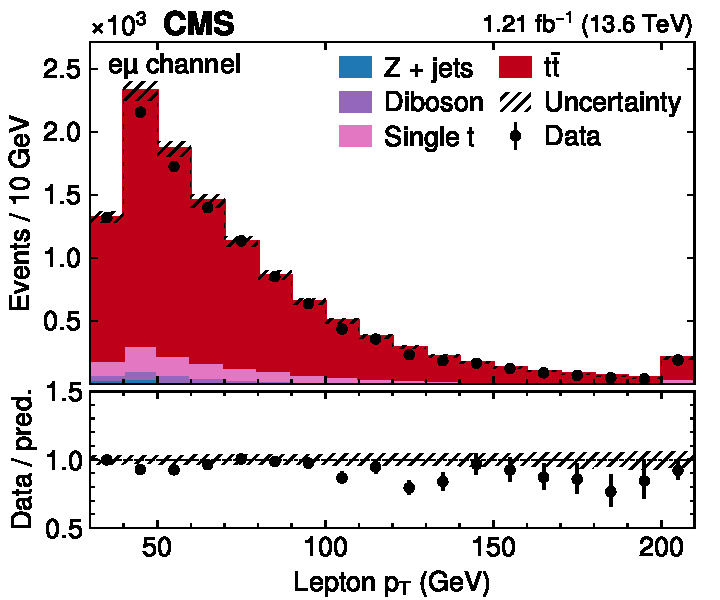
\includegraphics[width=0.49\textwidth]{figures/ttxs/lep_pt_em.pdf}
\hfill
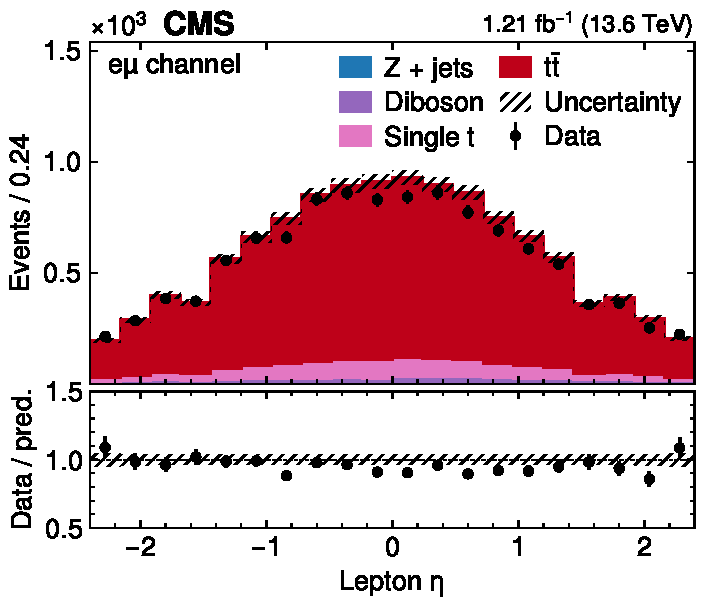
\includegraphics[width=0.49\textwidth]{figures/ttxs/lep_eta_em.pdf}
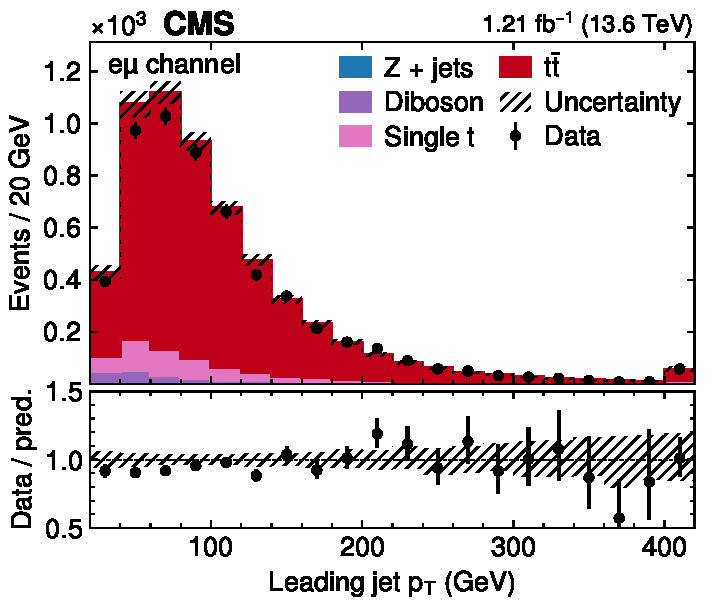
\includegraphics[width=0.49\textwidth]{figures/ttxs/1st_jet_pt_em.pdf}
\hfill
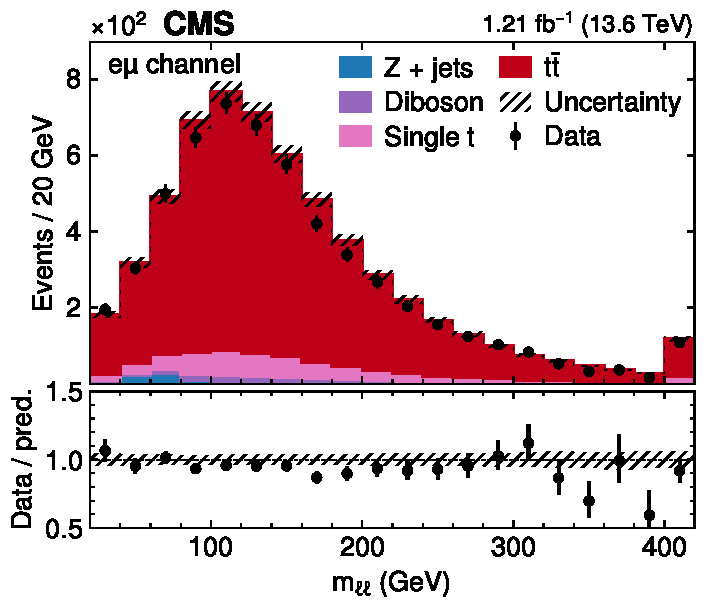
\includegraphics[width=0.49\textwidth]{figures/ttxs/mll_em.pdf}
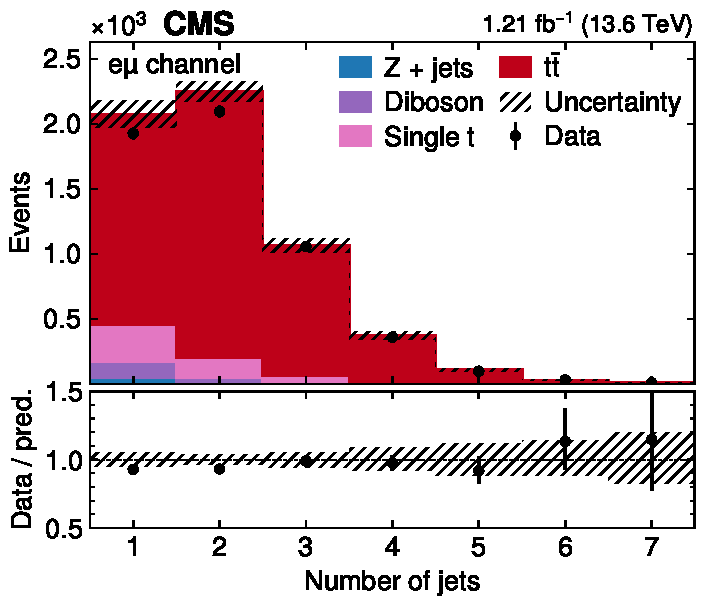
\includegraphics[width=0.49\textwidth]{figures/ttxs/njet_em.pdf}
\hfill
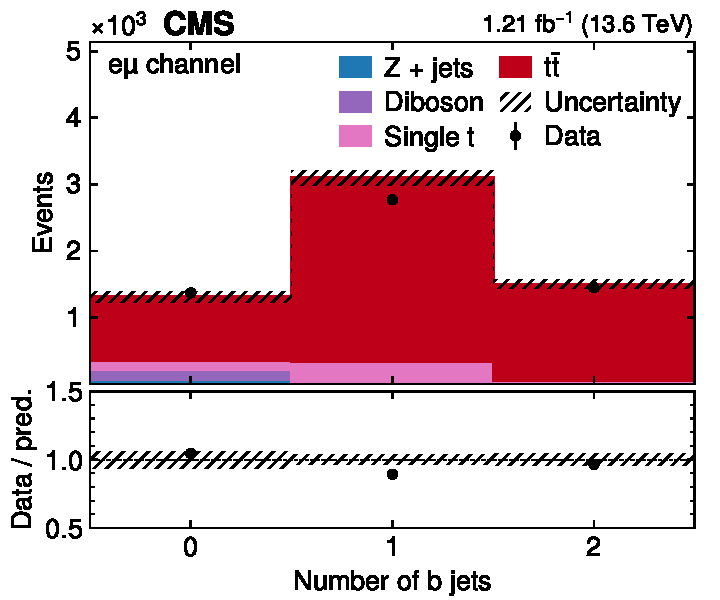
\includegraphics[width=0.49\textwidth]{figures/ttxs/nbtag_em.pdf}
\caption{
    \textbf{Control distributions in the \emu channel.} Shown are (from top left to bottom right) the distributions of \pt of both leptons, \abseta of both leptons, \pt of the leading jet, the invariant lepton mass \mll, the number of jets and the number of b jets. All figures show both data (black dots) and different simulated background processes (colored bars). For the latter, all corrections described in \cref{sec:ttxs:corrections} as well as post-fit b tagging scale factors (\cref{sec:ttxs:fitresults}) are applied, and the shaded area covers both statistical and systematic uncertainties. \textit{Figure taken from \citere{CMS:TOP-22-012}}.
}
\label{fig:ttxs:control_em}
\end{figure}

\begin{figure}[!hp]
\centering
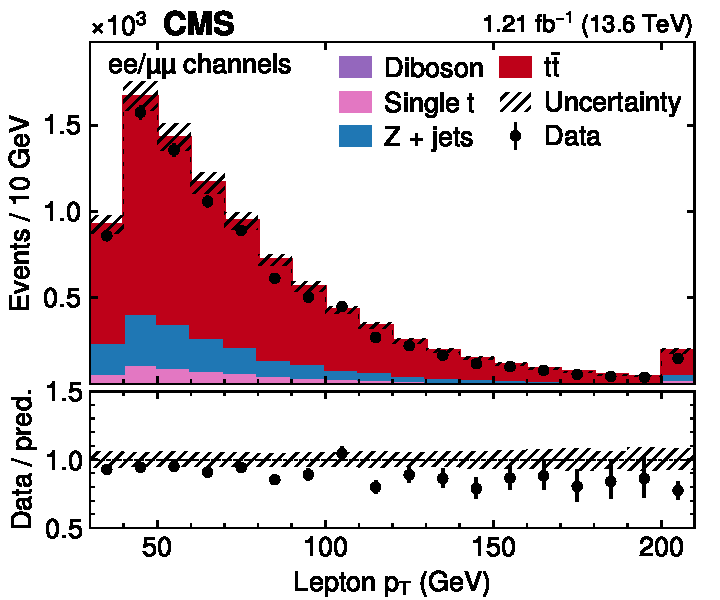
\includegraphics[width=0.49\textwidth]{figures/ttxs/lep_pt_eemm.pdf}
\hfill
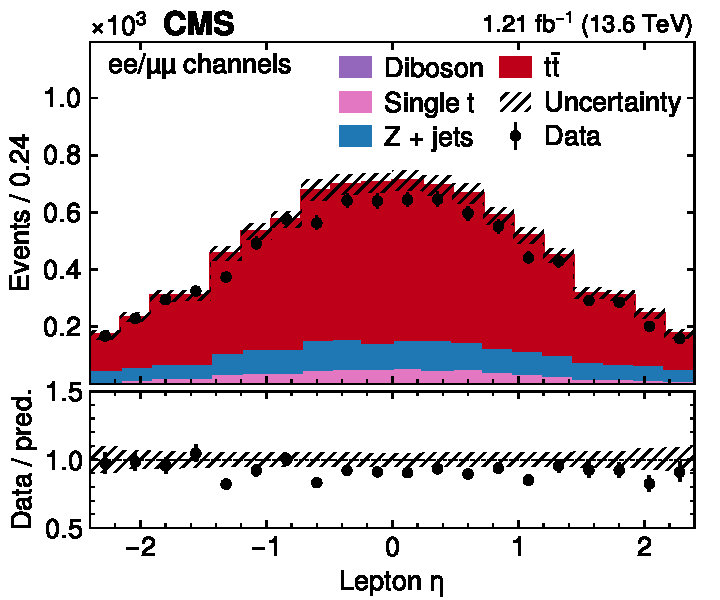
\includegraphics[width=0.49\textwidth]{figures/ttxs/lep_eta_eemm.pdf}
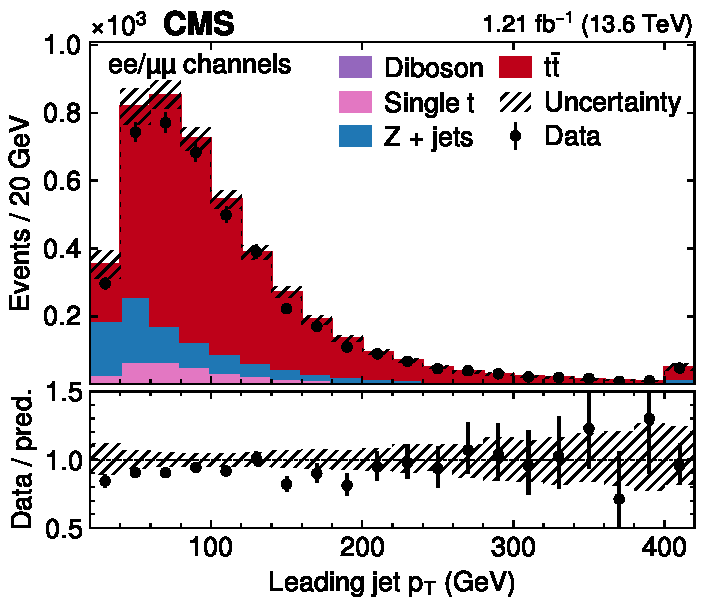
\includegraphics[width=0.49\textwidth]{figures/ttxs/1st_jet_pt_eemm.pdf}
\hfill
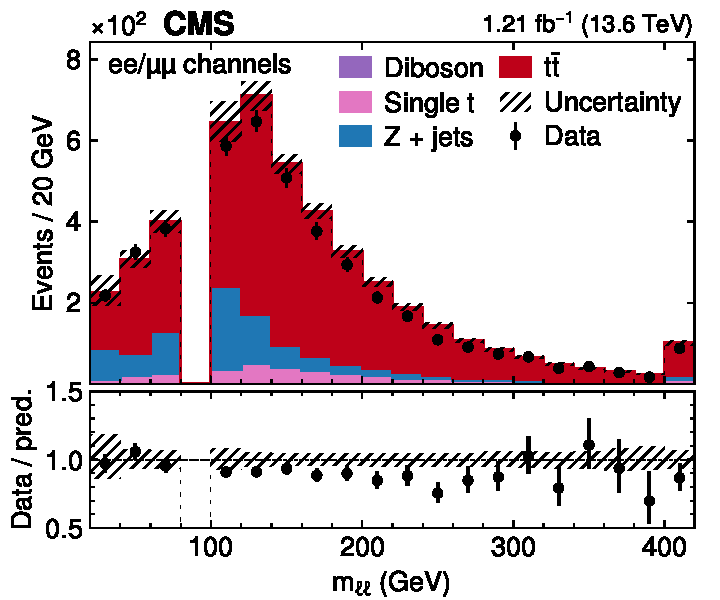
\includegraphics[width=0.49\textwidth]{figures/ttxs/mll_eemm.pdf}
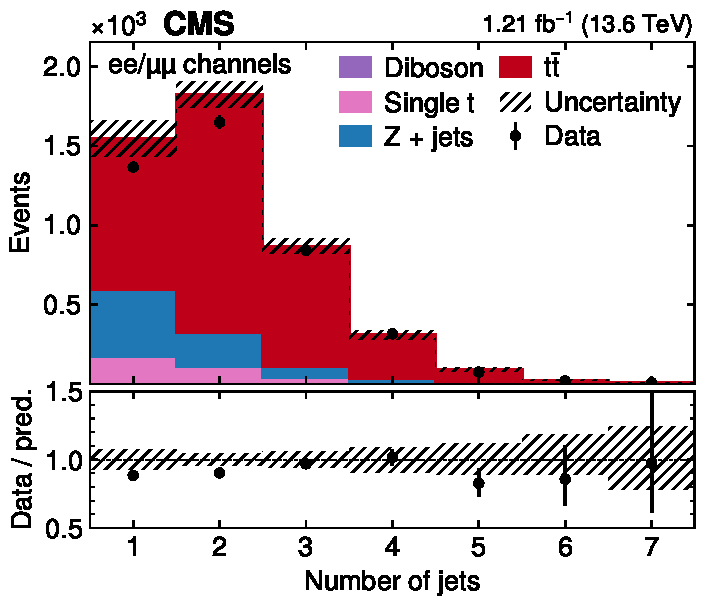
\includegraphics[width=0.49\textwidth]{figures/ttxs/njet_eemm.pdf}
\hfill
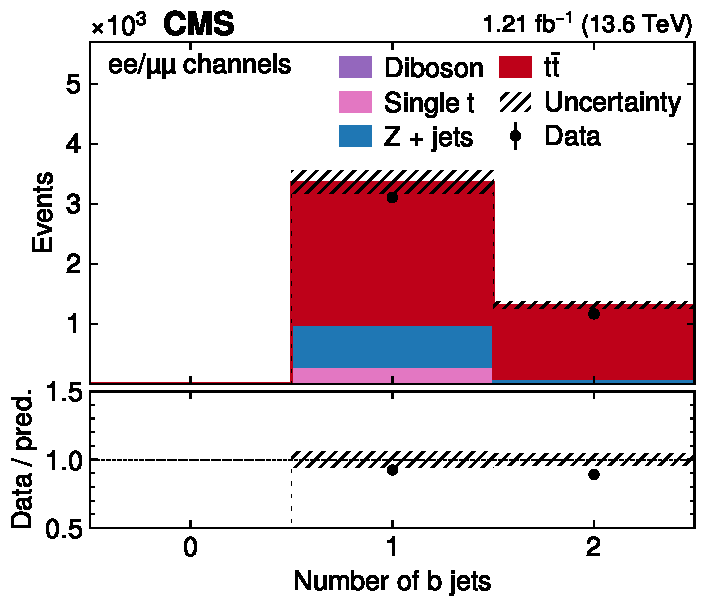
\includegraphics[width=0.49\textwidth]{figures/ttxs/nbtag_eemm.pdf}
\caption{
    \textbf{Control distributions in the \ee and \mumu channels.} The distributions are shown in the same manner as in Fig.~\ref{fig:ttxs:control_em}. \textit{Figure taken from \citere{CMS:TOP-22-012}}.
}
\label{fig:ttxs:control_eemm}
\end{figure}

\begin{figure}[!hp]
\centering
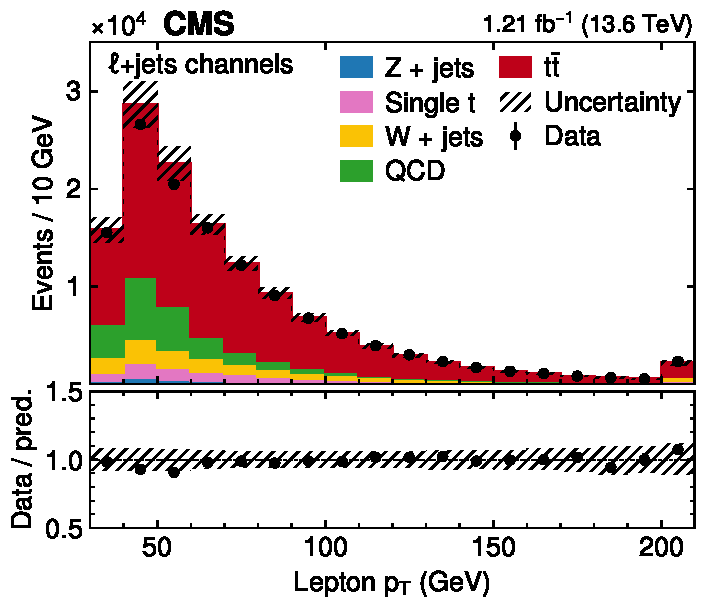
\includegraphics[width=0.49\textwidth]{figures/ttxs/lep_pt_lj.pdf}
\hfill
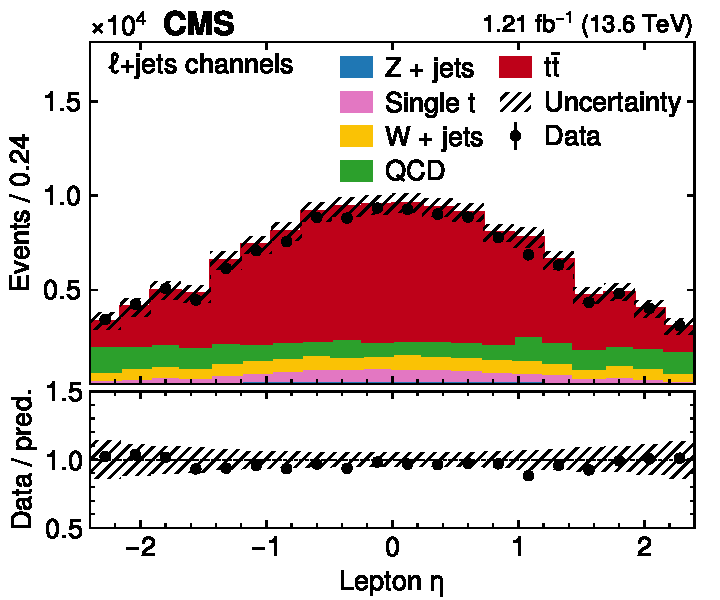
\includegraphics[width=0.49\textwidth]{figures/ttxs/lep_eta_lj.pdf}
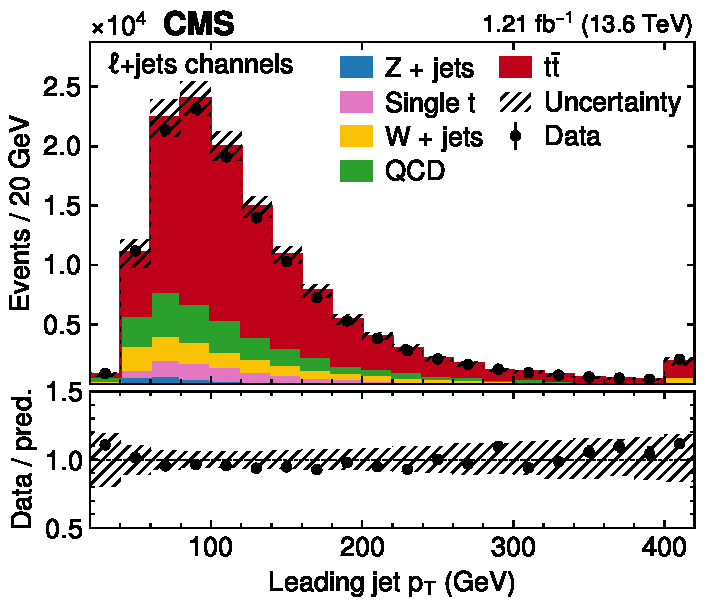
\includegraphics[width=0.49\textwidth]{figures/ttxs/1st_jet_pt_lj.pdf}
\hfill
\includegraphics[width=0.49\textwidth]{figures/ttxs/1st_jet_eta_lj.pdf}
\includegraphics[width=0.49\textwidth]{figures/ttxs/njet_lj.pdf}
\hfill
\includegraphics[width=0.49\textwidth]{figures/ttxs/nbtag_lj.pdf}
\caption{
   \textbf{Control distributions in the \ljets channels.} The distributions are shown in the same manner as in Fig.~\ref{fig:ttxs:control_em}, except for the center-right figure, which here shows \abseta of the leading jet. \textit{Figure taken from \citere{CMS:TOP-22-012}}.
}
\label{fig:ttxs:control_ljets}
\end{figure}

Good agreement between data and simulation within the full uncertainties is seen in all distributions.

%\section{Likelihood fit}
%\label{sec:ttxs:fit}


\section{Systematic uncertainties}
\label{sec:ttxs:systematics}

% required: general shape uncertainties, special treatment of btag uncertainty, special treatment of lepton uncs in free floating case, XS uncs, lumi unc.

In order to translate the distribution of observed and expected events into a result for the inclusive \ttbar cross section while taking into account all relevant sources of systematic uncertainties, a binned profile maximum likelihood fit as described in \cref{ch:stat} is performed using the tool \texttt{combine}~\cite{CMS:CAT-23-001}.
The parameter of interest (POI) used for this fit is the signal strength $r = \sigmatt / \sigmatt^{\text{pred}}$, i.e. the inclusive \ttbar cross section normalized to its theoretical prediction. A linear signal model is used as defined in \cref{eq:methods:linearsignal}, and the \ttbar cross section is extracted using its maximum likelihood estimate and uncertainty.

This section describes the considered systematic uncertainties, which can be divided into experimental uncertainties, arising from incomplete knowledge of the details of the detector and resulting differences between data and simulation, and theoretical uncertainties, which concern imperfect modeling of the underlying physical processes in the different event generators. %All of them will be described in this section.

All systematic uncertainties are included in the fit as nuisance parameters (NPs) as discussed in \cref{ch:stat}. In practice, NPs which encode shape effects on the considered observables are implemented using \textit{template morphing}, i.e. a smooth polynomial interpolation between the nominal shape and the shapes encoding the variations by $\pm 1$ standard deviations. NPs that encode only normalization effects are instead implemented as simple log-normal uncertainties. Both definitions can be found in detail in \citere{CMS:CAT-23-001}.

Special attention is given in this section to some experimental uncertainties which are important to this measurement. This includes the luminosity, which is the dominating uncertainty, as well as 
%the lepton identification and 
the b tagging uncertainties due to the special way they are treated in the fit.

\paragraph{Luminosity uncertainty}

In order to translate event yields into a result on any cross section, the total integrated luminosity is required as a calibration constant. Any experimental error on the luminosity will be directly transferred to the total error on the measurement, and thus minimizing the luminosity uncertainty is crucial for any cross section measurement.

For the data set used in this analysis, the total integrated luminosity was measured by the CMS Collaboration with an estimated uncertainty of 2.3\%. Of this number, 2.1\% is due to the calibration of the integrated luminosity, using the methods presented in \citere{CMS:LUM-17-003}.%The largest contribution comes from the so-called \textit{factorization bias}, which arises in the van der Meer method from the assumption that the transverse luminous area factorizes in the $x$ and $y$ coordinates, and from residual beam position deviations.

The agreement in the absolute scale is checked by comparing different independently calibrated luminosity measurements. The integrated luminosity measured with the hadronic forward calorimeter and the silicon pixel detector is found to agree at a level of better than 0.8\%.
Accounting for residual differences in time stability and linearity between the luminosity detectors results in a total uncertainty of 2.3\%. This preliminary estimate of the integrated luminosity at the time of publication was further validated using the yield of reconstructed Z bosons decaying into muon pairs~\cite{CMS:DP-2023-003}. After correcting for efficiencies and normalizing to the fiducial cross section predicted at NNLO with next-to-NNLL corrections, good agreement was observed.\footnote{Since publication of this result, a more precise luminosity measurement for 2022 data has become available in \citere{CMS:LUM-22-001-PAS}.}
%Taking additional contributions due to residual differences in the time-stability and linearity between the luminosity detectors into account leads to the full figure of 2.3\%.
%The preliminary estimate of the integrated luminosity at the time of publication was further cross-checked by using the yield of reconstructed Z bosons decaying into pairs of muons~\cite{CMS:DP-2023-003}, corrected for efficiencies and normalized to the fiducial cross section prediction calculated at NNLO with next-to-NNLL corrections applied, which also showed good agreement.\footnote{Since publication of this result, a more precise luminosity measurement for 2022 data has become available in \citere{CMS:LUM-22-001-PAS}.}

In contrast to all other uncertainties described below, the uncertainty in the integrated luminosity is not directly included in the likelihood fit, but rather treated as an external uncertainty and added in quadrature afterwards, since it is expected to factorize completely from all other uncertainties.
The impact of varying the normalization of the backgrounds estimated from simulation by the integrated luminosity uncertainty was found to be negligible.
% TODO.

\paragraph{b tagging uncertainty}

As mentioned in \cref{sec:ttxs:scalefactors}, the efficiency for correctly identifying a jet originating from a b quark (b tagging) is expected to be different in data and simulation. At the time of this measurement, directly after the start of Run 3, no general-purpose b tagging studies had been available. Thus, the approach adopted here is to consider the b tagging efficiency in data to be completely unknown and measure it concurrently with the cross section in the likelihood fit.

For this purpose, the probability for an event with $n_{\mathrm{jet}}$ selected jets to have $n_{\mathrm{b tag}}$ correctly identified b jets, depending on the assumed b tagging efficiency $\epsilon_b$, is assumed to be a multinomial of the form

\begin{equation}
\label{eq:ttxs:btags}
    P (n_{\mathrm{b tag}} | n_{\mathrm{jet}}) \propto \epsilon_b^{n_{\mathrm{b tag}}} (1 - \epsilon_b)^{ n_{\text{no tag}}}
\end{equation}

Here, $n_{\text{no tag}}$ is the number of true b jets in the event which fall into the acceptance of the selection, but fail to be tagged by \textsc{DeepJet}. It is estimated from MC simulation. %Note that this might be lower then the number of b jets expected from the physical process (e.g. 2 for \ttbar). 

By taking the ratio of eq. \ref{eq:ttxs:btags} in data and simulation, one can derive a per-event weight which corrects the number of b tags in MC:
%. From this, a shape template depending on $\epsilon_b$ in data is constructed and included in the fit as a nuisance parameter. It can be seen in Fig. ??.

\begin{equation}
%\begin{split}
\label{eq:ttxs:btagsf}
    w_b = \frac
    {(\epsilon_b^{\mathrm{data}})^{n_{\mathrm{b tag}}} (1 - \epsilon_b^{\mathrm{data}})^{n_{\text{no tag}}}}
    {(\epsilon_b^{\mathrm{MC}})^{n_{\mathrm{b tag}}} (1 - \epsilon_b^{\mathrm{MC}})^{n_{\text{no tag}}}} 
    = (f_b)^{n_{\mathrm{b tag}}} \, \left( \frac{1 - f_b \, \epsilon_b^{\mathrm{MC}}}{1 - \epsilon_b^{\mathrm{MC}}} \right)^{n_{\text{no tag}}}
%\end{split}
\end{equation}

Here, $f_b = \epsilon_b^{\mathrm{data}}/\epsilon_b^{\mathrm{MC}}$ is the unknown b tagging scale factor. It is left freely floating in the likelihood fit. This is technically implemented by producing shape templates from MC with $f_b$ varied up and down by a fixed value and interpolating in between. This shape template can be seen in \cref{fig:ttxs:btagsf}, where it is evident that the categorization in the number of b tags gives significant constraining power for $f_b$. In the 1b categories, the shape with respect to the number of jets deviates significantly from a flat variation proportional to $f_b$ as naively expected. This is because of out-of-acceptance jets, corresponding to the second factor in \cref{eq:ttxs:btagsf}.

\begin{figure}[ht]
    \centering
    \includegraphics[width=0.99\textwidth]{figures/ttxs/scalefactors/btagsf.pdf}
    \caption{
       \textbf{b tagging scale factor variation.} The effect of varying the b tagging scale factor $f_b$ in \ttbar MC by an arbitrary value of $\pm 0.1$, shown for the number of jets in the 11 fit categories.
    }
    \label{fig:ttxs:btagsf}
\end{figure}

%Note that any dependence of $\epsilon_b$ on the jet kinematics factorizes out as long as said dependency is the same in data and MC. Possible kinematic dependencies of the ratio $f_b$ are neglected; since no kinematic information is used in the fit, this is deemed acceptable.
Note that, since $f_b$ is taken to be a single number, this method only corrects the overall b jet efficiency and does not consider any dependence of $\epsilon_b$ on jet kinematics. Because this measurement uses the same jet quality requirements (particularly the same \pt cuts) in all channels, and assuming that the b jet \pt and $\eta$ spectra in the different channels are roughly similar, any kinematic dependence is effectively integrated out in the overall efficiency scale factor $f_b$. %The fact that the spectrum itself is not corrected is not considered an issue here since the likelihood fit does not use kinematic information directly.
The lack of corrections to the spectrum is not considered problematic in this context, as the likelihood fit does not rely directly on kinematic information.

\paragraph{Lepton identification uncertainty}

% TODO: the structure is kinda shit here - scale factors + uncertainty + cross check. maybe try to merge some of these?

The uncertainty assumed on the lepton identification scale factors comes from two different sources: First, an inherent uncertainty originating in the tag-and-probe method (as described in \cref{sec:ttxs:scalefactors}) is considered. It consists of statistical uncertainties from both data and simulation, a systematic uncertainty derived from a comparison with a different Z+jets simulation sample produced at NLO in QCD, and another systematic uncertainty due to the choice of fitting function. Together, they make up for an uncertainty of $\sim 0.8\% \, (0.5\%)$ on the electron (muon) scale factors in the bulk of the phase space, and can rise up towards $\sim 5\%$ for high lepton \pt.

Secondly, it is taken into account that the scale factor between data and simulation might be slightly different in the Z+jets selection used for the T\&P method and the \ttbar selection used for the measurement of the cross section. The most important reason for this is the requirement of (b tagged) jets in almost all considered categories, as well as the requirement for at least three jets in the lepton+jets channels. 
This effect has been studied at CMS in the past and the difference found to be less then 0.5\% for muons and 1.0\% for electrons. Taking a conservative approach, these values are used as an additional component in the respective uncertainties.

In the first, preliminary version of this measurement~\cite{CMS:TOP-22-012-PAS}, the dedicated lepton efficiency scale factors as measured with the T\&P method were not yet available, and a different approach was taken. Similar to the b tagging efficiency, the lepton efficiency scale factors were kept freely floating the likelihood fit. Due to the different dependency on the lepton efficiencies in the different lepton flavor channels, the fit was able to constrain the efficiencies to a precision of 2\%~\cite{CMS:TOP-22-012}. The resulting scale factors were later found to be in good agreement with those obtained from the T\&P method, serving as a valuable cross-check. However, this method ultimately led to less precision and was thus not used in the final result.
\todo{decide on removing as Alexander suggested}

\paragraph{Pileup uncertainty}

As described in \cref{sec:ttxs:scalefactors}, three different pileup-related variables are employed to reweight the simulation to the observed data, and the average of the three weights is used as the nominal value. This method is repeated using only one of the variables - the number of good reconstructed vertices $n_{\mathrm{PV}}$ - and the difference in expected yields treated as an uncertainty. 
This procedure was compared to the usual estimation of pileup-related uncertainties in CMS. There, the theoretical expectation for the number of interactions %is derived as a function of total inelastic proton-proton cross section, and the latter is than varied by its experimental uncertainty.
%It was found that the heuristic method used here leads to larger uncertainties, and can thus be considered more conservative.
is taken as the product of the instantaneous luminosity and the total inelastic cross proton-proton cross section of $\SI{69.2 \pm 3.2}{\milli\barn}$ at \sqrtsRII~\cite{CMS:LUM-17-003}. It was found that the heuristic method used here leads to
larger uncertainties than the one from the inelatic cross section, and can thus be considered more conservative.

\paragraph{Jet energy uncertainties}

Uncertainties in the jet energy calibration are split into 26 different sources concerning different experimental and theoretical effects, following the standard CMS procedure outlined in \citere{CMS:JME-13-004}. 17 of these sources are found to be non-negligible and included in the fit, while the others are indistinguishable from fluctuations due to limited MC statistics. These sources include, among others, uncertainties due to jet \pt resolution and jet flavor composition, statistical uncertainties in the derivations of the energy corrections, and residual differences between data and simulation.

\paragraph{Trigger uncertainties}

Since the trigger scale factors are derived using the tag-and-probe method in the same way as the lepton scale factors, similar uncertainties are applied, including the uncertainties of 0.5\% for muons and 1.0\% for electrons due to extrapolation between Z+jets and \ttbar topologies. The only difference is that in the dilepton channels the uncertainties need to be propagated according to \cref{eq:ttxs:triggersf}. This has the effect of greatly reducing the impact of the trigger uncertainties in those channels compared to the lepton ID uncertainties, since the nominal per-event trigger efficiency is already very close to one.

\paragraph{Matrix element scale uncertainties}

The theoretical predictions of both signal and background are calculated using matrix elements at either LO or NLO in perturbative QCD, matched to a parton shower. Since this effectively means truncating the perturbative expansion of the scattering amplitude at a given power in the strong coupling constant, the effect of higher-order terms is neglected in the calculation.

At the same time, the necessity of renormalization of divergent diagrams and factorization of non-perturbative contributions introduces non-physical parameters into the prediction in the form of the renormalization and factorization scales $\mu_R$ and $\mu_F$ (cf. \cref{sec:mc:me}). These parameters are usually set to typical energy scales of the considered process, and might also depend on the event kinematics (dynamic scales).

To estimate possible uncertainties due to these missing terms as well as due to the choice of scales, the scales $\mu_R$ and $\mu_F$ are varied separately by a factor of 2 up and down, and the resulting change in simulation is taken as an uncertainty in the form of shape templates \cite{Cacciari:2004}. %In order to not double-count uncertainties in the cross section prediction for the backgrounds (see below), but keep possible rate variations due to acceptance effects, the templates are normalized to the nominal cross section values before any selection cuts are applied. Different physical processes are considered to be uncorrelated since they are produced with different generators and at different orders. 
To avoid double-counting uncertainties in the background cross section predictions (see below) while still accounting for possible rate variations due to acceptance effects, the templates are normalized to the nominal cross section values before applying any selection cuts.

\paragraph{PDF uncertainties}

The PDFs used to evaluate the non-perturbative contribution of the proton-proton collision have systematic uncertainties attached. They are estimated by independently reweighting the simulation to 100 different replicas of the used NNPDF 3.1 PDF set and taking the envelope of the resulting changes, following the recommendations of the PDF4LHC working group \cite{Butterworth:2015oua}. Additionally, the effect of the choice of the strong coupling constant in the PDF is assessed using a similar reweighting, and attached as a separate nuisance parameter. Analogously to the matrix element uncertainties, the resulting variations are normalized before any selection cuts to keep acceptance and shape effects while not double-counting cross section changes.

\paragraph{Parton shower uncertainties}

The parton shower model used for the predictions is only accurate (at most) at LL and LC in QCD (cf. \cref{sec:mc:showering}) and thus requires appropriate uncertainties. For this purpose, the scales at which the strong coupling constant is evaluated are varied up and down by a factor 2 separately for initial and final state radiation and for different processes, and the resulting changes are propagated to the fit as shape templates.

\paragraph{ME/PS matching uncertainty}

For the simulation of the \ttbar signal, an additional uncertainty concerning the matching between matrix element simulation in \powheg and parton showering in \pythia is considered. This is done by varying the $h_{\mathrm{damp}}$ parameter in \powheg controlling the amount of radiation generated at matrix element level, following \citere{CMS:TOP-16-021}.

\paragraph{Top quark \pt uncertainty}

It has been shown in previous measurements of \ttbar differential cross sections that the \pt spectrum of the top quark is significantly softer in data than in the standard \powheg MC simulation~\cite{CMS:TOP-17-014,CMS:TOP-16-007,CMS:TOP-16-008}. This effect is propagated to the \pt spectra of the top decay products and can thus lead to misestimation of the acceptance due to lepton and b jet \pt requirements. Fixed-order predictions at NNLO in QCD and NLO in EW are known to largely alleviate the discrepancy~\cite{Czakon:2017wor}. Thus, a common strategy is to reweight the top quark \pt spectrum in MC simulation to the one extracted from such fixed-order predictions.

At the time of the measurement, fixed-order predictions at NNLO in QCD and NLO EW were available only for \sqrtsRII and could not be directly applied to the MC simulation at \sqrtsRIII. Instead, the simulation is left uncorrected for the nominal prediction, and a variation is constructed by calculating the ratio of the fixed-order prediction from \citere{Czakon:2017wor} and the \powheg MC simulation at \sqrtsRII, and applying it to the \powheg MC simulation at \sqrtsRIII. The difference between uncorrected prediction and the variation is assigned as an additional uncertainty, which is one-sided by construction.

\paragraph{Background cross section uncertainties}

For the cross sections of the different processes, log-normal rate uncertainties are assigned based on the process and order at which it was calculated. Separate 15\% uncertainties are used for the $t$-channel single-top and tW backgrounds since they are generated at NLO with a NNLO prediction for the cross section, while
for W+jets and Diboson, 30\% is used since these samples are only generated at LO. For Z+jets, this is reduced to 20\% due to the data-driven estimation of the normalization.
Additionally, for the fully data-driven QCD background, two separate nuisance parameters for the \ejets and \mujets channels are defined, covering a conservative uncertainty of 30\% each.

\paragraph{Background statistical uncertainties}

Finally, since the background in this measurement is estimated either using MC simulation or data-driven methods, an independent statistical uncertainty needs to be attached to each bin, reflecting the finite number of events it contains. This is done using the so-called \textit{Barlow--Beeston light} method~\cite{Barlow:1993dm}. For MC backgrounds, these uncertainties are minuscule. However, for the data-driven QCD background, they also contain the propagated statistical uncertainty due to the limited number of data events in the CRs, which is in general non-negligible.


\section{Fit results}
\label{sec:ttxs:fitresults}

\begin{figure}[!ht]
\centering
\includegraphics[width=0.99\textwidth]{figures/ttxs/prefithist.pdf}
\includegraphics[width=0.99\textwidth]{figures/ttxs/postfithist.pdf}

\caption{
   \textbf{Comparison of data and simulation before and after the fit.} The distribution of the number of jets in the different fit categories is shown for data and simulation before (top) and after the likelihood fit (bottom). The fit greatly improves the agreement and strongly constrains the background uncertainties. \textit{Figure taken from \citere{CMS:TOP-22-012}}.
}
\label{fig:ttxs:prepostfit}
\end{figure}

Performing the fit yields a \ttbar signal strength of $r = 0.959 \pm 0.025$, where the uncertainty includes statistical and all systematic contributions, except for the 2.1\% uncertainty on the luminosity. This corresponds to an inclusive \ttbar cross section of

\[
    \sigmatt = 881 \pm 23 \, \text{(stat+syst)} \pm 20 \, \text{(lumi)} \, \text{pb}.
\]

The result is in good agreement with the standard model prediction of $\sigmatt^{\text{pred}} = 924^{+32}_{-40} \, \text{pb}$.

Fig.~\ref{fig:ttxs:prepostfit} shows the agreement between data and simulation before and after the fit. It can be immediately seen that the fit greatly reduces the uncertainty on the prediction by constraining systematic uncertainties and simultaneously improves the agreement compared to the data. 

Of particular note here is the free-floating b tagging efficiency (compare sec.~\ref{sec:ttxs:systematics}), whose effect can be directly read off from the categorization in the number of b jets: Before the fit (Fig.~\ref{fig:ttxs:prepostfit} top), the event yield for two or more b jets is overestimated in the simulation, while the yield for zero b jets is underestimated. This suggests that the b tagging efficiency is slightly lower in the data than assumed in the simulation. Indeed, the fit confirms this: the b tagging scale factor between data and simulation in the phase space of this measurement is measured to be $f_b  = 0.980 \pm 0.009$. As a result, after the fit (Fig.~\ref{fig:ttxs:prepostfit} bottom), the event yields agree in all b jet categories.

\subsection{Statistical checks}

To better understand the sources of systematic uncertainty, as well as the contributions of the different measurement channels, the fit is repeated twice, restricted to either the dilepton or the \ljets channels. For both cases as well as the combination, the contribution of different groups of nuisance parameters is calculated by freezing the groups to their postfit values and repeating the fit, as explained in \cref{ch:stat}. It should be noted that this procedure does not take into account correlations between the groups, and thus the sum in quadrature of the separate components will in general not add up to the total uncertainty.

The results can be found in \cref{tab:ttxs:systematics}, where it can be seen how the combination of channels helps to reduce the total uncertainty: in the dilepton channels, the dominating uncertainties are the lepton identification uncertainty, which enters twice compared to the \ljets channels, as well as the statistical uncertainty of the data due to the relatively low branching ratio. In the \ljets channels, b tagging, JES, and pileup uncertainties dominate, reflecting the less clean selection and increased importance of jets. When the channels are combined, the uncertainty contribution of these groups lies inbetween the two separate numbers, showing how the channel combination represents a tradeoff between the advantages and disadvantages of either channel.

\begin{table}[!t]
\centering\renewcommand\arraystretch{1.1}
\begin{tabular}{l|c c c}
    Source & Full measurement & dilepton only & \ljets only\\
    \hline
    \hline
    Lepton ID efficiencies & 1.6 & 2.2 & 1.0 \\
    Trigger efficiency & 0.3 & \makebox[0pt][r]{$<$}0.1 & 0.5 \\
    JES & 0.6 & 0.7 & 1.1 \\
    b tagging efficiency & 1.1 & 0.8 & 2.1 \\
    Pileup reweighting & 0.5 & 0.2 & 1.1 \\
    ME scale, \ttbar & 0.5 & 0.4 & 0.5 \\
    ME scale, backgrounds & 0.2 & 0.1 & 0.3 \\
    ME/PS matching & 0.1 & 0.4 & 0.7 \\
    PS scales & 0.3 & 0.5 & 0.4 \\
    PDF and \alphas & 0.3 & 0.4 & 0.4 \\
    Top quark \pt & 0.5 & 0.3 & 0.5 \\
    tW background & 0.7 & 1.0 & 0.4 \\
    $t$-channel single-t background & 0.4 & \makebox[0pt][r]{$<$}0.1 & 0.5 \\
    Z+jets background & 0.3 & 0.2 & \makebox[0pt][r]{$<$}0.1 \\
    W+jets background & \makebox[0pt][r]{$<$}0.1 & \makebox[0pt][r]{$<$}0.1 & 0.2 \\
    Diboson background & 0.6 & 0.6 & \makebox[0pt][r]{$<$}0.1 \\
    QCD multijet background & 0.3 & -- & 0.5 \\
    Statistical uncertainty & 0.5 & 1.2 & 0.5 \\ \hline
    Combined uncertainty & 2.6 & 3.4 & 3.3 \\ \hline
    Integrated luminosity & 2.3 & 2.3 & 2.3 \\
\end{tabular}
\caption{
    \textbf{Sources of systematic uncertainty.} The relative per-cent contribution of different groups of sources of systematic uncertainty for the full measurement as well as for restrictions to the dilepton and \ljets channels only. They are calculated according to \cref{ch:stat} and do not take correlations between the different groups into account.
}
\label{tab:ttxs:systematics}
\end{table}

Furthermore, the nuisance parameter pulls, constraints and impacts, as defined in \cref{ch:stat}, are shown in \cref{fig:ttxs:impacts} for the channel combination. One can see how the electron identification scale factors, which are the leading impact, are constrained by the combination of channels, while the same is not true of the muon identification scale factors due to their lower prefit uncertainty.

\begin{figure}[!ht]
    \centering
    \includegraphics[width=0.9\linewidth]{figures/ttxs/impacts_v2.pdf}
    \caption{\textbf{Nuisance parameter pulls, constraints and impacts.} The expected and observed values are shown as shaded bands and error bars, respectively. Nuisance parameters are sorted by their observed impact on the signal strength $r$. For the b tagging scale factor, for which no prefit uncertainty is defined, the post-fit uncertainty is shown instead of the pull. \textit{Figure taken from the supplementary material of \citere{CMS:TOP-22-012}}.}
    \label{fig:ttxs:impacts}
\end{figure}


%\subsection{Lepton efficiency check}

\subsection{Top quark mass dependence}
\label{sec:ttxs:topmass}

An additional source of uncertainty that has not been considered so far is the choice of top quark mass in the \ttbar MC simulation. It affects the selection efficiency indirectly via the \pt cuts on leptons and jets, with higher top quark mass values leading to harder spectra and thus to larger efficiencies.

Contrary to other uncertainty sources, the top quark mass is not profiled in the likelihood fit. Instead, the dependence of the extracted \ttbar cross section is explicitly quantified as a function of the top quark mass by shifting its value in simulation by $\pm \SI{3}{\GeV}$ from its default of $\mt = \SI{172.5}{\GeV}$.
The extraction of \sigmatt is then repeated and the dependence on \mt extracted through a simple linear fit. This strategy has been taken in previous CMS and ATLAS \ttbar cross section measurements~\cite{CMS:TOP-17-001,ATLAS:2020aln}, and thus facilitates comparison with previous results.

For an upwards shift of $\Delta \mt = \SI{1}{\GeV}$, the \ttbar cross section is found to shift downwards by \SI{8.5}{\pb}, and vice versa. If one takes the current experimental uncertainty of \SI{0.3}{\GeV}~\cite{PDG:2022pth} as an allowed range for \mt, this would lead to an additional uncertainty on \sigmatt of 0.3\%.
% todo: impacts and GOF
% lepton SF consistency check
% tt curve

\section{Summary and Outlook}
\label{sec:ttxs:summary}

\begin{figure}[!ht]
    \centering
    \includegraphics[width=0.8\linewidth]{figures/ttxs/tt_curve.pdf}
    \caption{\textbf{Summary of \sigmatt measurements.} An overview of inclusive \ttbar cross section measurements at CMS at different center-of-mass energies~\cite{CMS:TOP-11-007, CMS:TOP-14-018, CMS:TOP-12-006, CMS:TOP-13-004, CMS:TOP-17-001, CMS:TOP-18-005, CMS:TOP-20-001, CMS:TOP-20-004} as well as comparison to the SM prediction~\cite{Czakon:2013goa}. This measurement is displayed as the red dot. \textit{Figure taken from \citere{CMS:TOP-22-012}}.}
    \label{fig:ttxs:ttcurve}
\end{figure}

In this chapter, the inclusive \ttbar cross section is measured for the first time at a center-of-mass energy of \sqrtsRIII. Data corresponding to an integrated luminosity of \lumiRIII from the beginning of LHC Run~3 are analyzed. Despite this comparatively small amount of data, a total precision of ca. 3\% with respect to the inclusive cross section is achieved.

\cref{fig:ttxs:ttcurve} compares the result of this chapter to other inclusive \ttbar cross section measurements performed by CMS at other center-of-mass energies~\cite{CMS:TOP-17-001, CMS:TOP-11-007, CMS:TOP-14-018, CMS:TOP-12-006, CMS:TOP-13-004, CMS:TOP-18-005, CMS:TOP-20-001, CMS:TOP-20-004}, as well as to the SM prediction~\cite{Czakon:2013goa}. The precision is comparable to other measurements at $\sqrt{s} = 7$, $8$, and $\SI{13}{\TeV}$, some of them with significantly higher integrated luminosities. All results are in agreement with the SM.

This measurement was designed specifically for the earliest data of Run~3, in order to achieve high precision without relying on a full suite of calibrations being available. In particular, b tagging and lepton efficiencies can be constrained in situ using the combination of dilepton and \ljets channels as well as the categorization by number of b-tagged jets. No large inconsistencies for any of the considered physics objects were found. The measurement was made public in September of 2022 just two months after the start of Run~3 and constituted the first public physics result of LHC Run~3. At the time, it provided a valuable first proof that CMS data taken in Run~3 were of high quality and ready for physics.

The next step for this result would be to transfer the technique developed in this work to well-understood data and high integrated luminosities in order to achieve the highest precision possible for \sigmatt. Such a measurement will certainly be dominated by systematic uncertainties, most importantly the luminosity and the lepton identification efficiencies (as already partly the case here). 
The channel combination method developed here could potentially help reduce the latter uncertainty through an in situ constraint, while the former is independent of the analysis strategy and requires more precise luminosity measurements for improvement. In addition, a more detailed study of the individual sources of uncertainty will likely be necessary to assess whether some can be reduced through improved calibrations.
%The channel combination method developed here could potentially help reduce the latter of these through an in situ constraint, while the former is orthogonal to the analysis strategy and its reduction requires more precise luminosity measurements. It will likely also be necessary to study the different sources of uncertainty in more detail, and investigate whether some of them can be reduced through more careful calibrations.

Additionally, one could try to use such a high-precision \ttbar cross section measurement to indirectly measure the top quark mass, one of the fundamental parameters of the Standard Model, by comparing the measured value of \sigmatt to SM predictions for different top quark masses. For this purpose, it would be important to reduce the dependence on the top quark mass in simulation (c.f. \cref{sec:ttxs:topmass}), for example by reducing the \pt requirements on leptons and jets as much as experimentally feasible. 
All of this leaves multiple parts for future studies to tread, which will be exciting to follow in the coming years as larger parts of the Run~3 data set are analyzed at CMS.
%All of this is, however, not part of this thesis and material for future work.
% what about outlook to higher lumi values? easy to do...


\chapter{Simulation of on-~and off-shell \ttbartitle production with \texorpdfstring{\bbfourl}{bb4l}}
\label{ch:bb4l}

\section{Introduction}

The accurate modeling of top quark production processes at the LHC is of crucial importance for precision measurements of top quark properties. In particular, the fact the top quark is an unstable colored resonance with a short lifetime presents challenges for correctly modeling its mass line shape as used for top mass and width measurements~\cite{Tarrach:1980up,Smith:1996xz,Hoang:2020iah}. Typically, the modeling is done with full NLO MC simulations matched to a parton shower (NLO+PS), and multiple such generators are available with different features and degrees of accuracy.

In this chapter, the predictions of some of these generators from the \powheg framework~\cite{Powheg:2004,Powheg:2007} are compared to each other, as well as to unfolded data measured in \citere{ATLAS:2018ivx}, for different variables relevant to top mass and/or width measurements. A particular focus is the generator \bbfourl \cite{Jezo:2016ujg}, which specifically improves the treatment of the unstable top resonance and of the interference between \ttbar and tW, and is described in detail in \cref{sec:bb4l:bb4l}. In this work, \bbfourl is implemented and validated for the first time in the CMS simulation setup. The comparison is done at the generator level, i.e. including parton showering and hadronization but not detector simulation and experimental reconstruction.

The results of this work have been published in a CMS public note as \citere{CMS:NOTE-2023-015}. Since the publication of this note, a new version of \bbfourl has been made available~\cite{Jezo:2023rht}. In this thesis, updated results including both versions will be shown.

\section{The Monte Carlo generator \texorpdfstring{\bbfourl}{bb4l}}
\label{sec:bb4l:bb4l}

\bbfourl ~\cite{Jezo:2016ujg,Jezo:2023rht} is a full NLO+PS MC generator for the process $pp \to b \bar{b} \ell^+ \ell^- \nu_\ell \bar{\nu}_\ell$, including all off-shell contributions. This includes the dilepton decay channel of both \ttbar and tW production, as well as non-resonant contributions involving Z or Higgs bosons, as shown in \cref{fig:bb4l:feynman}. Since these processes all lead to the same final state at NLO in QCD, they interfere which each other and cannot be easily separated. \bbfourl includes this interference by construction since it computes the full amplitude including all diagrams at once.

\begin{figure}[t]
    \centering
    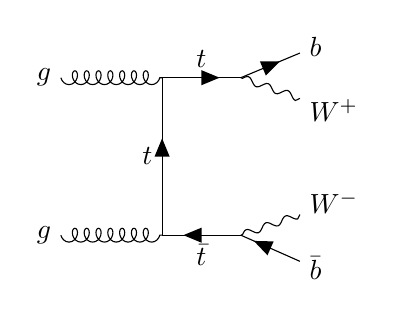
\begin{tikzpicture}[baseline=(current bounding box.center)]
      \begin{feynman}
        \vertex (i1) {\(g\)};
        \vertex [below=2.0 cm of i1] (i2) {\(g\)};
        \vertex [right=1.5 cm of i1] (a);
        \vertex [right=1.5 cm of i2] (b);
        \vertex [right=1.0 cm of a] (c);
        \vertex [right=1.0 cm of b] (d);
        \vertex [above right=0.15 cm and 0.75 cm of c] (fb1) {\(b\)};
        \vertex [below right=0.15 cm and 0.75 cm of c] (fW1) {\(W^+\)};
        \vertex [above right=0.15 cm and 0.75 cm of d] (fW2) {\(W^-\)};
        \vertex [below right=0.15 cm and 0.75 cm of d] (fb2) {\(\bar{b}\)};
        \diagram* {
          (i1) -- [gluon] (a),
          (i2) -- [gluon] (b),
          (c) -- [anti fermion, edge label'=\(t\)] (a) -- [anti fermion, edge label'=\(t\)] (b) -- [anti fermion, edge label'=\(\bar{t}\)] (d),
          (c) -- [fermion] (fb1),
          (c) -- [boson] (fW1),
          (d) -- [anti fermion] (fb2),
          (d) -- [boson] (fW2),
        };
      \end{feynman}
    \end{tikzpicture}
    \hfill
    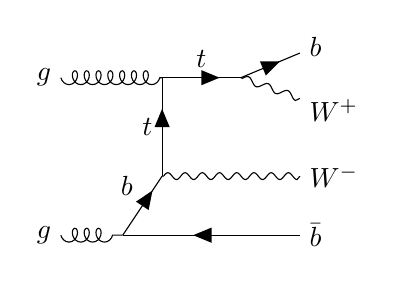
\begin{tikzpicture}[baseline=(current bounding box.center)]
      \begin{feynman}
        \vertex (i1) {\(g\)};
        \vertex [right=1.5 cm of i1] (a);
        \vertex [below=2.0 cm of i1] (i2) {\(g\)};
        \vertex [below=1.25 cm of a] (b);
        \vertex [right=1.0 cm of a] (c);
        \vertex [right=1.0 cm of i2] (d);
        \vertex [above right=0.15 cm and 0.75 cm of c] (fb1) {\(b\)};
        \vertex [below right=0.15 cm and 0.75 cm of c] (fW1) {\(W^+\)};
        \vertex [right=1.75 cm of b] (fW2) {\(W^-\)};
        \vertex [right=2.25 cm of d] (fb2) {\(\bar{b}\)};
        \diagram* {
          (i1) -- [gluon] (a),
          (i2) -- [gluon] (d),
          (c) -- [anti fermion, edge label'=\(t\)] (a) -- [anti fermion, edge label'=\(t\)] (b) -- [anti fermion, edge label'=\(b\)] (d),
          (c) -- [fermion] (fb1),
          (c) -- [boson] (fW1),
          (d) -- [anti fermion] (fb2),
          (b) -- [boson] (fW2),
        };
      \end{feynman}
    \end{tikzpicture}
    \hfill
    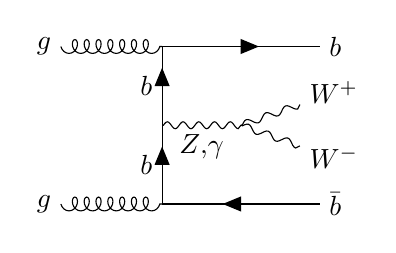
\begin{tikzpicture}[baseline=(current bounding box.center)]
      \begin{feynman}
        \vertex (i1) {\(g\)};
        \vertex [below=2.0 cm of i1] (i2) {\(g\)};
        \vertex [right=1.5 cm of i1] (a);
        \vertex [right=1.5 cm of i2] (b);
        \vertex [below=1.0 cm of a] (c);
        \vertex [right=1.0 cm of c] (d);
        \vertex [right=2.0 cm of a] (fb1) {\(b\)};
        \vertex [above right=0.15 cm and 0.75 cm of d] (fW2) {\(W^+\)};
        \vertex [below right=0.15 cm and 0.75 cm of d] (fW1) {\(W^-\)};
        \vertex [right=2.0 cm of b] (fb2) {\(\bar{b}\)};
        \diagram* {
          (i1) -- [gluon] (a),
          (i2) -- [gluon] (b),
          (fb1) -- [anti fermion] (a) -- [anti fermion, edge label'=\(b\)] (c) -- [anti fermion, edge label'=\(b\)] (b) -- [anti fermion] (fb2),
          (c) -- [boson, edge label'=\(Z\mathrm{,}\gamma\)] (d),
          (d) -- [boson] (fW1),
          (d) -- [boson] (fW2),
        };
      \end{feynman}
    \end{tikzpicture}
    \caption{\textbf{Feynman diagrams for \bbfourl.} Examples of Feynman diagrams for the $pp \to b \bar{b} W^+ W^-$ process as described by \bbfourl, including double-resonant (left), single-resonant (center) and non-resonant contributions (right). The decay of the W bosons into leptons is not shown for brevity.}
    \label{fig:bb4l:feynman}
\end{figure}

In addition, by considering the full amplitude instead of splitting it into production and decay, \bbfourl treats the top quark as an unstable resonance without approximations. It is implemented in the ``resonance-aware'' version of \powheg, called \powhegvres~\cite{Jezo:2015aia}, which includes the hardest QCD radiation also for unstable resonances - such as top quarks - in addition to the hardest initial state radiation always provided by \powheg. As a result, an event generated by \bbfourl can have up to three hard emissions at matrix element level. The correct description of these FSR emissions is relevant e.g. for observables related to the mass of the top quark, and can be challenging for parton showers, leading to large uncertainties.

This work investigates two different versions of \bbfourl. The first version is the one originally published in \citere{Jezo:2016ujg} and publicly available on the \powheg website~\cite{Powheg:website}. In the following, it will be referred to as \bbfourl v1.

The second version of \bbfourl was recently published in \citere{Jezo:2023rht}. Its most prominent feature compared to the previous version is the addition of the lepton+jets decay channel of \ttbar, i.e. the $b \bar{b} \ell \nu_{\ell} q \bar{q}'$ final state. Moreover, it includes several improvements to the dilepton final state, such as avoidance of spurious finite width effects and improved resonance history projectors (see \citere{Jezo:2023rht} for details). At the time of writing this thesis, the new code is not publicly available. A preview version was made available to the CMS collaboration by the authors, and the dilepton final state of this version - referred to as \bbfourl v2 - is shown in this work. The lepton+jets final state, on the other hand, was not ready for validation in the preview version, and so could not be included.

\section{Other \ttbartitle Monte Carlo generators}
\label{sec:bb4l:others}

The distributions predicted by \bbfourl are compared to three other MC generators for the \tttW final state, which are briefly presented in this section. All of these are implemented in \powhegvtwo, and as such do not contain explicit treatment of radiation in unstable resonances.

\subsection{\texorpdfstring{\hvq}{hvq}}

\hvq~\cite{Frixione:2007nw}, standing for \textit{heavy quark}, is the standard code used, at the time of writing, by both the ATLAS and CMS collaborations for producing \ttbar MC events. It applies the narrow-width approximation (NWA) to generate stable \ttbar pairs at NLO in QCD, with up to one additional ISR emission. The top quarks are then randomly smeared according to the top quark width, giving an approximate treatment of finite-width effects. Following this, the top quarks are decayed - in this case, in the dilepton channel for all lepton flavors - using internal \powheg routines~\cite{Frixione:2007zp}. These routines work at tree level at LO in QCD and preserve spin correlations. Further ISR emissions as well as all FSR emissions are provided by the parton shower.

\subsection{\texorpdfstring{\ST}{ST\_wtch}}

Since \hvq generates only the double-resonant \ttbar amplitude, a second generator has to be used alongside it for the single-resonant tW and \tttW interference contributions. Here, \ST~\cite{Re:2010bp} is used for this purpose. It works very similar to \hvq, also generating a stable tW pair in the NWA, smearing with the top width and decaying the particles using the same routines.

However, in order to at least approximately recover the full $b \bar{b} W^+ W^-$ amplitude, it is necessary to select a scheme for the treatment of the \tttW interference to prevent double-counting. Since the separation between \ttbar and tW is not well defined at NLO, such schemes will to some degree always be ad-hoc and ambiguous. Two such schemes are implemented for \ST, and both are compared in this work: in the first, called diagram removal (DR), all terms involving the square of double-resonant diagrams are simply removed from the squared amplitude. This is the most intuitive choice, but has the disadvantage of not being gauge invariant~\cite{Frixione:2008yi}. The second method, diagram subtraction (DS), keeps double-resonant diagrams in the squared amplitude, and subtracts a gauge invariant counter-term to remove the double counting~\cite{Tait:1999cf,Frixione:2008yi,Re:2010bp}. For both schemes, the prediction of \ST is added to the one of \hvq (together called \tttWsum) to produce distributions that can be compared to \bbfourl.

\subsection{\texorpdfstring{\ttb}{ttb\_NLO\_dec}}

The generator \ttb~\cite{Campbell:2014kua}, similar to \hvq, works in the NWA and thus generates stable \ttbar pairs with ad-hoc smearing. However, unlike \hvq, it is fully NLO-accurate not only in the production, but also in the decay of the top quarks. This means that, like \bbfourl, it generates up to one hard FSR emission per decaying top quark, leading to up to three hard emissions in the final state. 

It also provides an LO-accurate treatment of the \tttW interference by reweighting the generated \ttbar events to the full off-shell LO amplitude. Thus, like \bbfourl, it can be used on its own and does not need to be added together with e.g. \ST, but is expected to work at a lower accuracy since it includes more approximations.

\section{Technical setup}
\label{sec:bb4l:setup}

For all generators, LHE events were generated and then showered and hadronized with the multi-purpose generator \pythia. Wherever possible, the same settings were used for the different generators, an overview of which can be found in \cref{tab:bb4l:settings}. They are mostly identical to the default settings used by CMS for MC generation, as discussed in \citere{CMS:GEN-17-001}.

\begin{table}
\centering
\begin{tabular}{c c}
    Parameter & Value \\
    \hline
    \hline
    \multicolumn{2}{c}{\powheg settings} \\
    Top quark mass & \SI{172.5}{\GeV} \\
    Top quark width & \SI{1.33}{\GeV} \\
    \hdamp & $1.38 \, m_t$~\cite{CMS:TOP-16-021} \\
    PDF set & NNPDF 3.1~\cite{NNPDF:2017mvq}\\
    \hline
    \multicolumn{2}{c}{\pythia settings} \\
    \pythia version & 8.307 \\
    \pythia tune & CP5~\cite{CMS:GEN-17-001}\\
    \hline
    \multicolumn{2}{c}{\texttt{PowhegHooks} settings~\cite{Pythia:2022}} \\
    \texttt{POWHEG:veto} & \texttt{on} \\
    \texttt{POWHEG:pThard} & 0 \\
    \texttt{POWHEG:pTdef} & 1
\end{tabular}
\caption{\textbf{Generator settings.} An overview of the settings for \powheg and \pythia, as well as the matching between them, for all considered generators.}
\label{tab:bb4l:settings}
\end{table}

\subsection{Parton shower matching}
\label{sec:bb4l:matching_theory}

Special care has to be taken regarding the matching of the \powheg ME generators to the parton shower as provided by \pythia.  %In particular, since \powheg already generates events with one or more hard or soft emissions, depending on the process, these configurations must be removed in some form from the \pythia shower to prevent double-counting~\cite{Corke:2010zj}.
For \hvq and \ST, this is accomplished here using a shower veto as described in \cref{sec:mc:showering}, and technically implemented using the \texttt{PowhegHooks} module of \pythia. By default, this module can only handle one ISR emission at matrix element level, and thus needs to be extended for \bbfourl and \ttb, which also contain FSR emissions in the top decay. This was implemented by the \bbfourl authors in the \texttt{PowhegHooksBB4L} module as described in detail in \citere{FerrarioRavasio:2018whr}. An updated form of this module compatible with \bbfourl v2 is used here. Similarly to the ISR case, it is possible to directly start the shower at the energy scale of the \powheg emission, or alternatively employ a veto for emissions above this scale. The latter is used as the default option, and compared to the former in \cref{sec:bb4l:matching}.

%In the naive approach, this is achieved by starting the parton shower in \pythia only at the hardness scale of the emission generated by \powheg (sometimes called ``wimpy shower''). This way, only additional softer emissions are generated by the shower, and double-counting is avoided. However, this works only as long as the hardness scale definitions in \powheg and \pythia are the same. In practice, they are equal approximately but not exactly, leading to possible inaccuracies.

%A more thorough approach can be achieved by always starting the parton shower at the high kinematic limit (``power shower''), calculating the hardness according to the \powheg definition for each generated emission, and vetoing emissions with hardness larger than the emission generated by \powheg. For ISR emissions this method is implemented in \pythia  as part of the \texttt{PowhegHooks} module, and used for all generators considered here.

%For \hvq and \ST, which generate only ISR emissions at ME level, this treatment are sufficient. However, for \bbfourl and \ttb, the veto procedure has to be extended to the FSR emissions generated by \powheg in the top decay. This was implemented by the \bbfourl authors in the \texttt{PowhegHooksBB4L} module, a modified form of which is used here, and described in detail in \citere{FerrarioRavasio:2018whr}. Similarly to the ISR case, it is possible to directly start the shower at the hardness scale of the \powheg emission, or employ a veto for emissions above this scale. The latter is used as the default options, and compared to the former in \cref{sec:bb4l:matching}.

\subsection{Same-flavor leptons}
\label{sec:bb4l:sameflavor}

By default, both versions of \bbfourl generate only dilepton final states with opposite-flavor leptons (electrons, muons or $\tau$ leptons). This is because, in principle, there are additional diagrams contributing to the $b \bar{b} \ell^+ \ell^- \nu_\ell \bar{\nu}_\ell$ amplitude for same-flavor leptons, such as $b \bar{b} ZZ$ with $ZZ \rightarrow \ell^+ \ell^- \nu_\ell \bar{\nu}_\ell$, that are not included in \bbfourl.

In practice, the effect of these diagrams will be small, especially in experimental analyses where a cut is applied to reject resonant same-flavor lepton pairs close to the Z boson mass (compare \cref{sec:ttxs:channels}). To make sure that \bbfourl can be used in CMS for experimental analyses involving all lepton flavors, a relabeling procedure already included in \bbfourl is extended to also produce same-flavor lepton final states, neglecting the aforementioned diagrams. This procedure is used for all \bbfourl distributions shown in this chapter.

\section{Results}

\subsection{Comparison between generators}

In this section, the two \bbfourl versions are compared against each other, as well as to the alternative generators introduced in \cref{sec:bb4l:others}, for different observables. All of these comparisons are done after parton showering and hadronization, but without any detector simulation.

The package \rivet~\cite{Rivet:2019rhm} was used to analyze the events. For some observables, publicly available analysis packages were employed, which is stated in the captions of the figures where applicable. Furthermore, some observables include distributions at the jet level, which are obtained by running an anti-$k_\mathrm{T}$ algorithm with distance parameter $\Delta R = 0.4$ (AK4)~\cite{Cacciari:2008gp}.

\paragraph{Lepton observables} To begin the comparison, events with at least two leptons of opposite sign satisfying $\pt > \SI{20}{\GeV}$ and $\abseta < 2.4$ are selected. Photons surrounding the leptons in a small cone of $\Delta R < 0.1$, originating from photon radiation, are clustered together with the leptons (``dressed leptons''). The \pt distributions of the leading and subleading of these two leptons are shown in \cref{fig:bb4l:leppt}. They show good agreement between the generators within the renormalization and factorization scale uncertainties. \tttWsum using the DR scheme predicts a slightly harder lepton spectrum then the others, while the DS scheme agrees with \bbfourl and \ttb.

\begin{figure}[tp]
    \centering
    \includegraphics[width=0.49 \textwidth]{figures/bb4l/generators/MC_TTBAR_DILEP_SPINDENSITY_lep_pt_1.pdf}
    \hfill
    \includegraphics[width=0.49 \textwidth]{figures/bb4l/generators/MC_TTBAR_DILEP_SPINDENSITY_lep_pt_2.pdf}
    \caption{\textbf{Distributions of lepton \pt} of the leading (left) and subleading
      (right) lepton for
      \bbfourl v1 (red), v2 (aqua), \tttWsum with the DR (blue) and DS scheme
      (green), as well as \ttb (magenta). The shaded bands show the
      uncertainty due to scale variations, while the error bars show
      the statistical uncertainty. \textit{Figure adapted from \citere{CMS:NOTE-2023-015}}.}
    \label{fig:bb4l:leppt}
\end{figure}

The same trend can be seen in \cref{fig:bb4l:mll} for the invariant lepton mass \mll, both inclusively and split by lepton flavor channels. The per-channel distributions are all comparable within statistical uncertainties, which validates the extension to same-flavor leptons for \bbfourl presented in \cref{sec:bb4l:sameflavor}.

\begin{figure}[tp]
    \centering
    \includegraphics[width=0.49 \textwidth]{figures/bb4l/generators/MC_TTBAR_DILEP_SPINDENSITY_mll.pdf}
    \hfill
    \includegraphics[width=0.49 \textwidth]{figures/bb4l/generators/MC_TTBAR_DILEP_SPINDENSITY_mll_emu.pdf}
    \includegraphics[width=0.49 \textwidth]{figures/bb4l/generators/MC_TTBAR_DILEP_SPINDENSITY_mll_ee.pdf}
    \hfill
    \includegraphics[width=0.49 \textwidth]{figures/bb4l/generators/MC_TTBAR_DILEP_SPINDENSITY_mll_mumu.pdf}
    \caption{\textbf{Distributions of \mll} for all lepton flavors combined (upper left) as well as in the \emu (upper right), \ee (lower left) and \mumu channels (lower right), shown in the same manner as in \cref{fig:bb4l:leppt}. \textit{Figure adapted from \citere{CMS:NOTE-2023-015}}.}
    \label{fig:bb4l:mll}
\end{figure}

\paragraph{Jet observables} Next, some selected AK4 jet observables are compared. 
%For this purpose, the jets are obtained with an anti-$k_\mathrm{T}$ algorithm with distance parameter $\Delta R = 0.4$ (AK4)~\cite{Cacciari:2008gp}.
Jets containing a B hadron are identified as b jets using a ghost association technique~\cite{Cacciari:2007fd,Cacciari:2008gn}. 

\begin{figure}[tp]
    \centering
    \includegraphics[width=0.49 \textwidth]{figures/bb4l/generators/MC_TTBAR_DILEP_SPINDENSITY_njet.pdf}
    \hfill
    \includegraphics[width=0.49 \textwidth]{figures/bb4l/generators/MC_HFJETS_ptBJetLead.pdf}
    \caption{\textbf{Number of jets and b jet \pt}. Distributions of the inclusive number of AK4 jets (left) and the \pt of the leading b jet (right, \rivet analysis \texttt{MC\_HFJETS}), shown in the same manner as in \cref{fig:bb4l:leppt}. \textit{Figure adapted from \citere{CMS:NOTE-2023-015}}.}
    \label{fig:bb4l:jets1}
\end{figure}

\begin{figure}[tp]
    \centering
    \includegraphics[width=0.49 \textwidth]{figures/bb4l/generators/MC_HFJETS_efracB.pdf}
    \hfill
    \includegraphics[width=0.49 \textwidth]{figures/bb4l/generators/MC_HFDECAYS_avg_rho_B_jet.pdf}
    \caption{\textbf{b fragmentation and jet shape.} Distributions of the b quark fragmentation (left, \rivet analysis \texttt{MC\_HFJETS}) and the average differential b jet shape (right, \rivet analysis \texttt{MC\_HFDECAYS}), shown in the same manner as in \cref{fig:bb4l:leppt}. \textit{Figure adapted from \citere{CMS:NOTE-2023-015}}.}
    \label{fig:bb4l:jets2}
\end{figure}

%\cref{fig:bb4l:jets1} shows the inclusive number of jets and the \pt of the leading b jet for the different cases. Several differences are observable here both between the two versions of \bbfourl and between \bbfourl and the other generators. For the number of jets, these are mostly covered by the scale uncertainties, while for the b jet \pt, there is an uncovered discrepancy at very low \pt. 
\cref{fig:bb4l:jets1} shows the inclusive jet multiplicity and the transverse momentum of the leading b jet for the different generator setups. Several differences can be observed, both between the two versions of \bbfourl and between \bbfourl and the other generators. For the jet multiplicity, the variations are largely covered by the scale uncertainties. However, for the leading b jet transverse momentum, a discrepancy remains at very low \pt that is not accounted for by these uncertainties.
It is interesting to note that the number of jets agrees well between \tttWsum and \bbfourl v2, while \bbfourl v1 and \ttb disagree and predict a larger number of jets. The origin of these discrepancies, especially between the \bbfourl versions, is not yet understood and subject of discussion with the authors of the program.

Next, \cref{fig:bb4l:jets2} shows the b quark fragmentation, defined as the fraction of energy of the central B hadron in a jet compared to the total jet energy, as well as the average differential b jet shape $\langle \rho (R) \rangle$, which is the transverse momentum density of the particles making up the b jet as a function of its radius $R$. Both of these variables are sensitive to final-state radiation from the top decay, and are thus expected to be affected by the full NLO calculation performed by \bbfourl. It can be seen that both versions of \bbfourl predict softer b jet spectra and wider jets than both \tttWsum and \ttb, which can be interpreted as more FSR emissions being generated. Notably, this effect cannot be solely due to the inclusion of hard FSR emissions in \bbfourl since these are also present in \ttb.

In general, all of these trends for \bbfourl (softer lepton and b jet spectra as well as wider jets) agree with what was observed in Refs.~\cite{FerrarioRavasio:2018whr,ATLAS:PHYS-PUB-2021-042}, but differ from the results initially reported in \citere{Jezo:2016ujg}.

\paragraph{Invariant b$\ell$ mass} A common proxy observable to use for measurements of the top quark mass in dilepton events is the invariant mass of a b jet and a lepton, \mbl. To do so, a procedure is needed to unambiguously assign the leptons and b jets (of which there might be varying numbers per event depending on the event selection) to each other. Here, exactly two b jets per event are required, and the so-called minimax mass is used, defined as

\begin{equation}
    \mblminimax = \min{ \left[  \max{ \left( m_{b_1 \ell_1},
          m_{b_2 \ell_2} \right) }, \max{ \left( m_{b_1 \ell_2},
          m_{b_2 \ell_1} \right) } \right] }.
\end{equation}

This prescription amounts to maximizing the invariant mass over the two b-$\ell$ pairs in the event, and then minimizing it over the two possible assignments of b jets and leptons. It is notable in that, for double-resonant \ttbar events, it shows a kinematic cutoff at a value of $\sqrt{\smash[b]{m_t^2 - m_W^2}} \approx \SI{150}{\GeV}$. As a result, the tail above this cutoff is sensitive to single-resonant tW events as well as \tttW interference and thus to the top quark width.

\begin{figure}[tp]
    \centering
    \includegraphics[width=0.49 \textwidth]{figures/bb4l/generators/ATLAS_2018_I1677498_d03-x01-y01.pdf}
    \caption{\textbf{Distribution of \mblminimax}, shown in the same manner as in \cref{fig:bb4l:leppt}. ATLAS data from \citere{ATLAS:2018ivx} is overlaid as black dots, and the \rivet routine from said reference was used to obtain the distributions. \textit{Figure adapted from \citere{CMS:NOTE-2023-015}}.}
    \label{fig:bb4l:mbl}
\end{figure}

\cref{fig:bb4l:mbl} shows the distribution of \mblminimax, again for all considered cases. It can be seen that both versions of \bbfourl are in good agreement with each other, and are also in agreement with \ttb except for the lowest bin. Unfolded ATLAS data taken from \citere{ATLAS:2018ivx} is overlaid on top of the predictions, and shows good agreement for both \bbfourl and \ttb. 
In the tail, the two interference handling schemes for \tttWsum show significant differences as expected, with \bbfourl and \ttb lying between them. Since \bbfourl is expected to provide a more accurate prediction of the interference then either scheme, this validates that using the difference of the schemes as an uncertainty covers the true values, as is done in many CMS and ATLAS measurements. Going forward, such uncertainties could be dropped from future measurements by using \bbfourl predictions directly.

\paragraph{Top quark reconstruction} Finally, in order to directly study the effects on top quark observables, a simple generator-level top quark reconstruction is performed. To do so, two dressed leptons and two b jets are selected as before, while the two neutrinos in the dileptonic top decay are taken from truth-level information. The W bosons are reconstructed from the neutrinos and charged leptons according to the lepton charge, and then combined with the b jets by choosing the pairs for which the difference $\Delta m_t$ between the invariant masses is minimal. 

This reconstruction procedure is not equivalent to a full experimental reconstruction, in which neutrinos are measured only as missing transverse momentum and thus cannot be directly assigned to the leptons. It also does not include any detector resolution effects. However, it does take into account the effects of FSR in the top decay by considering the full b jets instead of parton-level b quarks, which is why it was chosen for the comparison.

\begin{figure}[tp]
    \centering
    \includegraphics[width=0.49 \textwidth]{figures/bb4l/generators/MC_TTBAR_DILEP_SPINDENSITY_anytop_mass.pdf}
    \hfill
    \includegraphics[width=0.49 \textwidth]{figures/bb4l/generators/MC_TTBAR_DILEP_SPINDENSITY_anytop_pt.pdf}
    \caption{\textbf{Top quark line shape and \pt.} Distributions of the reconstructed top quark mass (left) and \pt (right), summed for both top and antitop quark, shown in the same manner as in \cref{fig:bb4l:leppt}. \textit{Figure adapted from \citere{CMS:NOTE-2023-015}}.}
    \label{fig:bb4l:top}
\end{figure}

\cref{fig:bb4l:top} shows the resulting distributions for the top quark mass and \pt. It can be seen that the different generators show different line shapes for the top quark mass: \bbfourl predicts a small shift towards lower values compared to \tttWsum for both interference handling schemes as well as \ttb, and also predicts significantly lower amounts of off-shell tops with masses below the pole mass compared to \tttWsum. Both of these facts are important for precision top mass measurements, in which such shifts can influence the final fit results. The presence of these differences is expected: due to the use of the NWA for both \tttWsum and \ttb, the top line shape can only be modeled approximately in these generators, while \bbfourl provides a true NLO-accurate description. It can furthermore be seen that the two \bbfourl versions are not in perfect agreement with each other, though the difference is within the scale uncertainties.

For the top quark \pt, on the other hand, any trend in the comparison between the generators is covered by the scale uncertainties, though \bbfourl does seem to again predict softer \pt spectra than the other generators, consistent with the trends observed for the lepton \pt and \mll.

\begin{figure}[tp]
    \centering
    \includegraphics[width=0.49 \textwidth]{figures/bb4l/generators/MC_TTBAR_DILEP_SPINDENSITY_ttbar_mass.pdf}
    \hfill
    \includegraphics[width=0.49 \textwidth]{figures/bb4l/generators/MC_TTBAR_DILEP_SPINDENSITY_ttbar_pt.pdf}
    \caption{\textbf{Kinematics of the \ttbar system.} Distributions of the reconstructed invariant mass (left) and \pt (right) of the \ttbar system, shown in the same manner as in \cref{fig:bb4l:leppt}. \textit{Figure adapted from \citere{CMS:NOTE-2023-015}}.}
    \label{fig:bb4l:ttbar}
\end{figure}

Lastly, the invariant mass and \pt distributions of the \ttbar system as a whole are shown in \cref{fig:bb4l:ttbar}. For \mtt, no clear trend can be seen for any of the considered generators. The \pt of the \ttbar system, on the other hand, shows significant differences both between the two \bbfourl versions and between \bbfourl and the other generators (which agree with each other). It should be noted that, since the initial state of the \pptt process has no \pt\footnote{Non-zero \pt of the incoming partons can be modeled with transverse momentum distributions~\cite{Boer:2011fh}, but this is not considered here.}, this variable is exactly zero at LO in QCD, and consequently determined only by emissions at NLO and beyond. As a result, it is expected to be sensitive to the NLO calculation and matching between matrix element and parton shower.

\subsection{Comparison of FSR matching settings}
\label{sec:bb4l:matching}

Complementary to the previous generator comparisons, this section investigates the effect of the matching between matrix element and parton shower for FSR in \bbfourl. As explained in \cref{sec:bb4l:matching_theory}, two principal options are available to match \bbfourl to \pythia in the used module \texttt{PowhegHooksBB4L}: In the first and nominal approach (denoted ``FSR veto''), the parton shower is started at the kinematic limit, and FSR emissions that lie above the \powheg energy scale of the relevant emission from the top decay as generated by \powheg are vetoed.

In the second approach (``Res. scale''), the shower is directly started at the energy scale of the \powheg FSR emission. This neglects the fact that the hardness scale definitions used in \powheg and \pythia as ordering variables are similar but do not match exactly. When the \pythia emission is only slightly softer (by the \pythia definition) than the \powheg emission, it is thus possible that it is in fact harder than the \powheg emission by the \powheg definition, leading to double-counting. Similarly, an emission that is only slightly harder by the \pythia definition and is thus not generated might in fact be softer by the \powheg definition, leading to under-counting.

In order to demonstrate the importance of correct parton shower matching, a third case (``Kin. limit'') is considered, in which the parton shower for FSR emissions is started naively at the kinematic limit without any veto procedure specifically directed at \bbfourl. This approach is thus expected to double-count FSR emissions.

The comparison in this section has been performed with \bbfourl v1. The matching for ISR emissions, done by \texttt{PowhegHooks}, is left identical between the three cases, as given in \cref{tab:bb4l:settings}.

\begin{figure}[tp]
    \centering
    \includegraphics[width=0.49 \textwidth]{figures/bb4l/matching/ADDED_top_mass.pdf}
    \hfill
    \includegraphics[width=0.49 \textwidth]{figures/bb4l/matching/MC_HFJETS_efracB.pdf}
    \caption{\textbf{Comparison of FSR matching settings.} Distributions of the reconstructed top quark mass (left, same as in \cref{fig:bb4l:top}) and the b quark fragmentation (right, same as in \cref{fig:bb4l:jets2}), for \bbfourl with different FSR matching settings as explained in the text (\cref{sec:bb4l:matching}). The shaded bands show scale uncertainties. \textit{Figure taken from \citere{CMS:NOTE-2023-015}}.}
    \label{fig:bb4l:matching}
\end{figure}

\cref{fig:bb4l:matching} shows the distributions of the top quark mass, reconstructed the same as before, and the b fragmentation for the different matching choices. Both of these observables were chosen for their sensitivity to FSR effects. It can be seen that the options ``FSR veto'' and ``Res. scale'' agree reasonably well with each other, with the top mass line shape showing a small shift between them within the scale uncertainties. This implies that the mismatch between the \powheg and \pythia energy scale definitions has a subleading effect in practice. On the other hand, the naive ``Kin. limit'' approach shows a large discrepancy due to its double-counting of FSR emissions, highlighting the importance of correct FSR matching procedures for NLO generators.

\subsection{Recoil in top decay}
\label{sec:bb4l:recoil}

In the simple parton shower in \pythia, there is a well-known problem affecting the virtualities of heavy unstable colored resonances, such as the top quark, in the treatment of FSR emissions in the resonance decay~\cite{Brooks:2019xso}. In particular, when performing a gluon emission off the decaying top quark and thus changing a $t \rightarrow Wb$ configuration to $t \rightarrow Wbg$, there is an ambiguity on how to distribute the recoil imposed by the gluon between the top decay products (W and b quark) such that the four-momentum of the $Wbg$ system is conserved.

\pythia 8.307, which is the version used for the previous studies in this chapter, offers two different treatments for this problem, which amount to assigning the recoil to only the W (``recoil to W'') or only to the b quark (``recoil to b''). Both of these are approximations, since a true treatment would distribute the recoil between the W and b quark in some form. CMS, and thus the studies previously shown in this chapter, use the ``recoil to b'' option.

Since \pythia 8.310, a third option (``recoil to top'') has been made available via the setting \texttt{TimeShower:recoilStrategyRF}. For this option, the W is chosen as the recoiler at first, but the emissions are then reweighted in such a way as to approximate the radiation pattern expected in a true resonance-aware shower~\cite{Brooks:2019xso}. It has been found in \citere{ATLAS:2022jbw} that the difference between this improved method and the old ones can have a substantial impact on top mass proxy observables and consequently measured top mass values, and there have been discussions on whether such a difference should be included as a systematic uncertainty.

This problem, in its core, is an issue of the parton shower and not the ME generator. Nonetheless, \bbfourl is expected to alleviate some of the ambiguities since it always includes the hardest gluon emission in each top decay at the ME level, where no question of assigning the recoil is raised. For subsequent and thus subleading emissions, the issue in principle still persists.

To estimate the effect of the top recoil in \bbfourl and compare it to \tttWsum, events from both generators are re-showered in \pythia 8.310 with the two choices of setting
\begin{align*}
\begin{split}
  \texttt{TimeShower:recoilStrategyRF = 1} &\quad \text{(``recoil to b'')} \quad \text{and} \\
  \texttt{TimeShower:recoilStrategyRF = 2} &\quad \text{(``recoil to top'')}.
\end{split}
\end{align*}
\bbfourl v2 is used for this comparison, and all other settings are kept at the nominal. For \tttWsum, only the DR scheme is considered for the interference handling.

\begin{figure}[tp]
    \centering
    \includegraphics[width=0.49 \textwidth]{figures/bb4l/recoil/MC_TTBAR_DILEP_SPINDENSITY_anytop_mass.pdf}
    \hfill
    \includegraphics[width=0.49 \textwidth]{figures/bb4l/recoil/MC_HFJETS_efracB.pdf}
    \caption{\textbf{Comparison of top recoil strategies.} Distributions of the reconstructed top quark mass (left, same as in \cref{fig:bb4l:top}) and the b quark fragmentation (right, same as in \cref{fig:bb4l:jets2}), for \bbfourl and \tttWsum with two different recoil treatments, as defined in the text (\cref{sec:bb4l:recoil}). The shaded bands show scale uncertainties.}
    \label{fig:bb4l:recoil}
\end{figure}

The results are shown in \cref{fig:bb4l:recoil} for the reconstructed top mass and the b quark fragmentation. Large differences are visible between the two recoil strategies for \tttWsum, as expected from Refs.~\cite{Brooks:2019xso,ATLAS:2022jbw}. For \bbfourl, on the other hand, the differences are very small, and lie within the scale uncertainties for the top quark mass. This implies that the effect of the recoil in subleading emissions is negligible in \bbfourl for the shown observables. As a result, \bbfourl circumvents the problem of top recoil that can otherwise be significant for \ttbar analyses.
\todo{After discussion with Afiq I am not really convinced whether these results are actually correct... In particular, are we sure that the recoil strategy option in pythia works correctly when matched to bb4l? Simone is unfortunately no longer around to ask. Should I remove it?}

\section{Summary and Outlook}

In this chapter, several generator-level studies of the MC generator \bbfourl, which generates the full $b \bar{b} \ell^+ \ell^- \nu_{\ell} \bar{\nu}_{\ell}$ final state including \tttW interference and off-shell top effects at NLO in QCD, have been presented. \bbfourl has been compared to other common \ttbar generators, namely \hvq, \ST (with two interference handling schemes) and \ttb, for different lepton, (b) jet and reconstructed top quark observables. For \mblminimax, \bbfourl agrees well with ATLAS data from \citere{ATLAS:2018ivx}, improving greatly upon the two interference handling schemes DR and DS for \tttWsum. For the reconstructed top quark mass, \bbfourl shows a significant shift compared to \tttWsum. In addition, two different \bbfourl versions have been compared, finding slight differences within scale uncertainties, and the matching of ME and parton shower as well as the treatment of the top recoil in \bbfourl have been studied further.

These studies represent valuable information for the choice of \ttbar MC generator in upcoming CMS measurements. For analyses in which \ttbar and tW are major backgrounds, \bbfourl can help reduce uncertainties originating in the \tttW interference treatment, and provide a more accurate description when off-shell regions of phase space are probed. This is briefly explored in \cref{sec:ah:gennps} in the context of a search for \ttbar bound state effects, which are naturally located in an off-shell-region. 
%Furthermore, \bbfourl will be of use when the \pptt process is instead the signal of a measurement. 
Furthermore, \bbfourl will be crucial for a simultaneous top mass and width measurement using MC templates, as originally proposed in \citere{FerrarioRavasio:2018whr}, in CMS. Alternatively, one might perform an differential \tttWsum cross section measurement, where \bbfourl could be used to unfold the data to generator level. 
%However, both of these ideas are outside the scope of this thesis, and are left for future work.

\chapter{Search for heavy scalar or pseudoscalar bosons in \ttbartitle final states}
\label{ch:ah}

\section{Introduction}
\label{sec:ah:intro}

Having studied \ttbar production at the energy frontier of \sqrtsRIII in \cref{ch:ttxs} as well as the modeling of off-shell top quarks in \cref{ch:bb4l}, this chapter is dedicated to a precision analysis of \ttbar using the large, well-studied Run~2 data set at \sqrtsRII, in the context of a search for new scalar or pseudoscalar bosons.

Additional spin-0 particles are predicted in many attractive extensions of the Standard Model, and can be searched for in \ttbar final states at the LHC if the new states are heavy (i.e. have a mass larger than $2\mt$), electrically neutral, and exhibit Yukawa-like couplings to fermions (see \cref{sec:theory:ah}). A generic model for such states with either pseudoscalar (A) or scalar (H) couplings to top quarks was given in \cref{eq:theory:lag_ah}.

In addition, \ttbar bound state effects are expected in the SM in several calculations, with a pseudoscalar component dominating at the LHC as discussed in \cref{sec:theory:etat}. 
Since additional BSM particles and bound state effects are expected to lead to similar experimental signatures, it makes sense to search for them for using the same methods.
%Since the experimental invariant mass resolution for the \ttbar final state is rather coarse, additional BSM particles and bound state effects are expected to lead to similar experimental signatures, and it thus makes sense to search for them for using the same methods.

%and searches for such particles at the LHC have potential of discovering hints for new physics. Oftentimes, such models predict Yukawa-type couplings for the new particles to SM fermions, which scale with the fermion mass. It is thus natural to search for interactions of new spin-0 states with the heaviest fundamental particle in the SM: the top quark.

%In particular, if the mass of any such new state is larger than double the top quark mass, it can decay to a \ttbar final state. This decay channel will be dominant in many scenarios. If the new state is produced in gluon fusion, the resulting process will interfere with SM \ttbar production as discussed in \cref{sec:theory:ttbar}, leading to an interference pattern in the invariant \ttbar mass that can be probed experimentally.

%To do so, a generic model describing the new particles is defined, containing two new spin-0 states A and H which both couple solely to the top quark via a pseudoscalar (for A) and a scalar (for H) Yukawa interaction. The Lagrangian reads

%\begin{equation}
%\label{eq:ah:lagrangian}
%\begin{split}
%    \mathcal{L}_{\AH} =& \, \frac{1}{2} (\partial_\mu A ) (\partial^\mu A ) +\frac{\mA^2}{2} A^2  
%    + i  \gAtt \, \frac{\mt}{v} \bar t  \gamma_5 \, t  \, A \\
%    & + \frac{1}{2} (\partial_\mu H ) (\partial^\mu H ) +\frac{\mH^2}{2} H^2  
%    -  \gHtt \, \frac{\mt}{v} \bar t \, t  \, H \,
%\end{split}
%\end{equation}

%Here, \mA and \mH are the masses of the new particles, \gAtt and \gHtt are the coupling modifiers for the top quark Yukawa couplings, \mt is the top quark mass, and $v$ is the vacuum expectation value of the SM Higgs boson. 

%This model assumes that the two states A and H do not mix, which is equivalent to the assumption that there is no \CP violation [??]. Apart from this assumption, it is fully generic and can be mapped onto any of the models discussed in \cref{sec:theory:ah}, provided that only couplings to the top quark are considered. This makes it ideal for an experimental search, as results presented using this model can be easily reinterpreted in various models of interest.

%In addition to the masses and coupling modifiers, the decay widths \wA and \wH of the two particles are also considered as free parameters, yielding six free parameters total. This is because, due to interactions with other SM particles besides the top quark, or with additional BSM particles, concrete models (e.g. the 2HDM) will predict different decay widths then the natural width expected in the simplified model. In particular, if either or both of the particles is to be considered a dark matter mediator, it will have a significant branching ratio to dark matter particles, increasing its absolute width.

This chapter presents such a search for new spin-0 states with either scalar or pseudoscalar interactions with the top quark, using the full Run~2 data set with an integrated luminosity of \SI{138}{\fbinv} at the CMS experiment. It follows up on a similar search done using only \SI{35.9}{\fbinv} of data taken in 2016~\cite{CMS:HIG-17-027}. Similar searches have also been published by ATLAS, one with \SI{20.3}{\fbinv} of data taken at $\sqrt{s}=\SI{8}{\TeV}$~\cite{ATLAS:2017snw} and one with \SI{140}{\fbinv} of data taken at $\sqrt{s}=\SI{13}{\TeV}$~\cite{ATLAS:2024vxm}.

The work done as part of this thesis focused on the dilepton decay channel of \ttbar, which is thus described in detail in~\cref{sec:ah:setup,sec:ah:ttbarweights,sec:ah:mereweighting,sec:ah:systs,sec:ah:prefit}. A significant excess of events is observed at invariant masses close to the \ttbar threshold, which is interpreted either as a pseudoscalar \ttbar bound state (\cref{sec:ah:etat,sec:ah:parityscan,sec:ah:checks}) or as an additional scalar or pseudoscalar boson (\cref{sec:ah:bestfitah}). For the latter interpretation, exclusion limits for a large mass range are also presented in \cref{sec:ah:limits}. Following this, the dilepton channel is combined with a similar analysis of the \ljets decay channel, which is discussed in \cref{sec:ah:combination}, and exclusion regions are provided for the presence of either one or two additional bosons. The results of this work are briefly compared in \cref{sec:ah:comparison} to preliminary ATLAS results in \citere{ATLAS:CONF-2025-008} which confirmed this measurement, to earlier ATLAS results in \citere{ATLAS:2024vxm} in which no excess was observed, and to other \ttbar measurements. Finally, a summary and outlook are given in \cref{sec:ah:summary}.

The results presented here were first made public as a Physics Analysis Summary~\cite{CMS:HIG-22-013-PAS}, and later submitted to \textit{Reports on Progress in Physics} in an updated form in two parts: first in \citere{CMS:TOP-24-007} focusing solely on the interpretation of a \ttbar bound state, and second in \citere{CMS:HIG-22-013} focusing on the interpretation in terms of additional bosons. 
They build upon the framework developed in \citeres{Anuar:PhD,Rubenach:PhD}, with this work consisting of 
%They are the continuation of a previous PhD thesis~\cite{Rubenach:PhD}, in which the analysis strategy of the dilepton channels as well as the procedure of obtaining exclusion limits for additional bosons was designed. Following up on this, the contribution of the work at hand consists of 
the implementation of matrix element reweighting for the signal simulation (\cref{sec:ah:mereweighting}), the simulation and scrutinization of the \ttbar bound state signal (\cref{sec:theory:etat}), the comparison with other MC generators for the \ttbar continuum (\cref{sec:ah:gennps}), the interpretation of the observed excess in terms of \ttbar bound states or additional bosons including all corresponding cross-checks (\cref{sec:ah:excess}), the combination with the \ljets channel (\cref{sec:ah:combination}), the comparison to other results (\cref{sec:ah:comparison}), and the preparation of the results for publication in Refs.~\cite{CMS:HIG-22-013} and \cite{CMS:TOP-24-007}.

\section{Analysis setup}
\label{sec:ah:setup}

This section describes the analysis strategy in the dilepton channels, consisting of the considered data sets, object definitions, event selection criteria, corrections and reconstruction algorithms.

\subsection{Data sets}
\label{sec:ah:datasets}

\paragraph{Experimental data} 
The analysis is performed using the full CMS Run~2 ultra-legacy (UL) data set, which is the final, re-reconstructed and recalibrated data set recommended by CMS for physics analyses. It is split into the three data taking years of Run~2: 2016, 2017 and 2018, where 2016 is further split into two parts, denoted ``2016pre'' and ``2016post", because of a modification of the silicon strip tracker readout chip settings that affects the efficiency of the track hit reconstruction during the 2016 data-taking period~\cite{CMS-DP-2020-045}.

A similar combination of dilepton and single-lepton triggers as in \cref{sec:ttxs:datasets} is used for all years, with the \pt thresholds varying slightly between data taking eras, as shown in \cref{tab:ah:triggers}. 

\begin{table}
\centering
\begin{tabular}{c|c|c}
    Trigger & Year & Lepton \pt requirement \\
    \hline
    \hline
    \multirowcell{3}{single-e} & 2016 & e~($\pt > \SI{27}{\GeV}$) \\
    & 2017 & e~($\pt > \SI{35}{\GeV}$) \\
    & 2018 & e~($\pt > \SI{32}{\GeV}$) \\
    \hline
    \multirowcell{3}{single-\textmu} & 2016 & \textmu~($\pt > \SI{24}{\GeV}$) \\
    & 2017 & \textmu~($\pt > \SI{27}{\GeV}$) \\
    & 2018 & \textmu~($\pt > \SI{24}{\GeV}$) \\
    \hline
    \multirowcell{2}{\emu} & \multirowcell{2}{all} & e~($\pt > \SI{12}{\GeV}$) and \textmu~($\pt > \SI{23}{\GeV}$) or \\
    & & e~($\pt > \SI{23}{\GeV}$) and \textmu~($\pt > \SI{8}{\GeV}$) \\
    \hline
    \ee & all & $\text{e}_1$~($\pt > \SI{23}{\GeV}$) and $\text{e}_2$~($\pt > \SI{12}{\GeV}$) \\
    \hline
    \mumu & all & $\text{\textmu}_1$~($\pt > \SI{17}{\GeV}$) and $\text{\textmu}_2$~($\pt > \SI{8}{\GeV}$)
\end{tabular}
\caption{\textbf{Trigger \pt thresholds.} Overview of the used triggers in the three data taking years, as well as their lepton \pt thresholds.}
\label{tab:ah:triggers}
\end{table}

\paragraph{Background simulation}
Since the final state of the signals considered in this analysis are the same as in the SM \ttbar background, it is clear that a large irreducible background is expected. As a result, it is essential that the SM Monte Carlo simulation is as both theoretically precise and has sufficient statistics, and that any remaining imprecisions are covered by the systematic uncertainty model.

The SM \ttbar background is again simulated at NLO in QCD, employing the narrow-width approximation (NWA) with a Breit-Wigner smearing for the top decay, using the MC generator package \powhegvtwo and interfaced to \textsc{Pythia 8} for showering, as discussed in detail in \cref{sec:mc:ttbar}. Equivalent settings as in \cref{sec:ttxs:datasets} and \cref{sec:bb4l:setup}, corresponding to the CMS defaults, have been used. To achieve the necessary precision, the NLO simulation is reweighted to higher orders in both QCD and electroweak (EW) processes, which is described in \cref{sec:ah:ttbarweights}.

In addition, several minor backgrounds are included, a summary of which can be found in \cref{tab:ah:simulation}. Of note here is the Z+jets background, which is simulated at NNLO in QCD using the MiNNLO method in \powhegvtwo~\cite{Monni:2019whf,Monni:2020nks}. It was found here that the higher-order corrections are relevant to the analysis especially for low values of the invariant dilepton mass \mll. Most processes are normalized to cross sections predicted at higher orders of QCD where available, which can be found in \cref{tab:ah:crosssections}.

\begin{table}
    \centering\renewcommand\arraystretch{1.2}
    \begin{tabular}{c|c|c}
     Process & QCD order & ME Generator \\
     \hline
     \hline
     \ttbar & NLO & \powhegvtwo (\texttt{hvq}~\cite{Frixione:2007nw}) \\
     tW & NLO & \powhegvtwo (\texttt{ST\_wtch}~\cite{Re:2010bp}) \\
     \Zgamma+jets & NNLO & \powhegvtwo (\texttt{Zj} MiNNLO~\cite{Monni:2019whf,Monni:2020nks}) \\
     $t$-channel single top & NLO & \powhegvtwo (\texttt{ST\_tch}~\cite{Alioli:2009je}) + \textsc{MadSpin}~\cite{Artoisenet:2012st} \\
     $s$-channel single top & NLO & \amcatnlo \\
     $\ttbar \mathrm{W}$ & NLO & \amcatnlo \\
     $\ttbar \mathrm{Z}$ & NLO & \amcatnlo \\
     WW, WZ \& ZZ & LO & \pythia 8.2 \\
     \hline
     \AH signal & LO & \amcatnlo \\
     \etat signal & LO & \amcatnlo
\end{tabular}
\caption{\textbf{Simulated background and signal samples.} An overview of the different background and signal processes considered, as well as the theoretical order in QCD and the ME generator used to simulate them. For all samples, \textsc{Pythia 8.2} is used for showering and hadronization.}
\label{tab:ah:simulation}
\end{table}

\begin{table}
    \centering\renewcommand\arraystretch{1.2}
    \begin{tabular}{c|c|c|c}
         Process & Cross section (pb) & Order & Program / reference \\
         \hline
         \hline
         \ttbar & 833.9 & NNLO+NNLL & Top++~\cite{Czakon:2011xx} \\
         tW & 71.7 & NNLO (approx.) & \cite{Kidonakis:2021vob} \\
         $t$-channel single top & 217.0 & NLO & Hathor~\cite{Aliev:2010zk,Kant:2014oha} \\
         $s$-channel single top & 10.3 & NLO & Hathor~\cite{Aliev:2010zk,Kant:2014oha} \\
         $\ttbar \mathrm{W}$ & 0.64 & NLO & \amcatnlo \\
         $\ttbar \mathrm{Z}$ & 0.75 & NLO & \amcatnlo \\
         $\Zgamma\mathrm{+jets} \rightarrow \ell\ell$, & \multirowcell{2}{$24.7 \times 10^3$} & \multirowcell{2}{NNLO} & \multirowcell{2}{FEWZ~\cite{Melnikov:2006kv,Li:2012wna}}  \\
         $\mll > \SI{10}{\GeV}$ & & & \\
         WW & 118.7 & NNLO & \cite{Gehrmann:2014fva} \\
         WZ & 47.1 & NLO & MCFM~\cite{Campbell:2010ff} \\
         ZZ & 16.5 & NLO & MCFM~\cite{Campbell:2010ff}
    \end{tabular}
    \caption{\textbf{Cross sections for background processes at \sqrtsRII.} The cross sections used for the normalization of background processes, as well as the orders in QCD at which they were computed. Where applicable, cross sections are given as the sum of the process and its charge conjugate.}
    \label{tab:ah:crosssections}
\end{table}

\paragraph{Signal simulation}

The signal for the general \AH model described in \cref{sec:ah:intro} is generated at LO in QCD using \amcatnlo with a custom Universal FeynRules Output (UFO) model. The $\mathrm{pp} \to \AH \to \ttbar$ resonance and the \AH-SM interference are simulated separately, and both are again showered with \textsc{Pythia 8}. In order to cover the phase space of the \AH model, the signals are generated for all combinations of the following values of the \AH masses and widths:

\begin{equation}
\begin{split}
    m_{\AH} &\in \{ 365, 400, 500, 600, 800, 1000 \} \, \si{\GeV} \\
    \Gamma_{\AH} / m_{\AH} &\in \{ 2.5, (5), 10, 25 \} \, \%
\end{split}
\end{equation}

Samples with a width of $5\%$, indicated by the bracket, were generated only for a mass of \SI{400}{\GeV}, which leads to 38 signal points total. In addition, samples for the pseudoscalar case only were generated with

\begin{equation}
    \mA \in \{ 450, 550, 700, 900 \} \, \si{GeV}, \quad \wA / \mA = 9 \, \%.
\end{equation}

All of these samples were combined and reweighted at matrix element level to obtain phase space points between these mass and width values, as described further in \cref{sec:ah:mereweighting}.

Furthermore, signal samples for possible \ttbar bound state effects are generated using the color-singlet \etat and \chit models as defined in \cref{sec:theory:etat}, using custom UFO models implemented in \amcatnlo and again showered with \pythia.
The branching ratio of $\mathrm{W} \rightarrow \ell \nu$ is taken to be $11.1\%$, corresponding to the default value used by \amcatnlo.

For all signal and background samples, the detector response is simulated with \textsc{Geant 4} and the full CMS simulation and reconstruction chain as described in \cref{sec:mc:detector} is performed.

\subsection{Object definition}
\label{sec:ah:objects}

\paragraph{Leptons} 

All electrons and muons are required to have $\abseta < 2.4$ and $\pt > \SI{20}{\GeV}$, corresponding to a less stringent cut than in \cref{ch:ttxs}. Similar to \cref{sec:ttxs:objects}, electrons in the transition region between barrel and endcaps in the ECAL, corresponding to $1.44 < |\eta_{\mathrm{SC}}| < 1.57$, are removed, and additional ID criteria are applied for both types of leptons.

For electrons, instead of a cut-based ID as in \cref{sec:ttxs:objects}, the multivariate classifier (MVA)-based ID described in \citere{CMS:EGM-17-001} is used at a working point giving 90 \% background rejection. This ID already includes an isolation requirement as part of the MVA training, and no further requirement is applied.

For muons, on the other hand, the same cut-based ID from \citere{CMS:MUO-16-001} as in \cref{sec:ttxs:objects}, also at the tight working point, is used, and the same \Irel requirement using a cone size of $\Delta R < 0.4$ is applied in addition.

\paragraph{Jets} 

Like in \cref{sec:ttxs:objects}, jets are reconstructed using the anti-$k_T$ algorithm~\cite{Cacciari:2008gp} with a distance parameter of $0.4$. They are required to fulfill $\pt > \SI{20}{\GeV}$, $\abseta < 2.4$, and have a minimum distance of $\Delta R > 0.4$ from all leptons passing the above criteria in the event. The Charged Hadron Subtraction (CHS) method~\cite{CMS:PRF-14-001} is used to remove hadrons that originate from pileup from the jet clustering.

Additional ID criteria are applied to reject jets originating in detector noise and reconstruction failures~\cite{CMS:2020ebo}. They consist of requirements on the multiplicities of the different jet constituents (charged hadrons, neutral hadrons, and electrons or photons) as well as their energy fractions relative to the total jet energy. The required values are centrally provided depend on the jet \abseta as well as on the analysis era. In total, a genuine jet efficiency of about 99 \% is achieved, while about 99.9 \% of noise jets are rejected in the relevan \abseta range~\cite{CMS:2020ebo}.

The \textsc{DeepJet} algorithm~\cite{DeepJet:2020}, same as in \cref{sec:ttxs:objects}, is used to identify jets originating from the showering and hadronization of b quarks. The medium working point of \textsc{DeepJet} in CMS is chosen, which has a b jet identification efficiency of 77 \%, as well as a misidentification rate of 15 \% for c quark jets and of 2 \% for light quark and gluon jets~\cite{CMS:BTV-16-002}.

\paragraph{Missing transverse momentum}

In the dileptonic decay of \ttbar, the two neutrinos leave the detector unseen, leading to a loss of information. However, their combined transverse momentum can be inferred through the missing transverse momentum \ptmissvec, defined as the negative vectorial sum of all reconstructed objects (jets, leptons and photons)~\cite{CMS:JME-17-001}. As with the jets, hadrons likely to originate from pileup are removed from the calculation of \ptmissvec using the CHS method~\cite{CMS:PRF-14-001}. Along with the leptons and jets, \ptmissvec will be used to reconstruct the \ttbar system.

\subsection{Event selection}

Events are selected with exactly two leptons of opposite electric charge and sorted into three channels (\ee, \emu and \mumu) by lepton flavor, similar to \cref{sec:ttxs:channels}. The two leptons need to fulfill $\pt > \SI{25}{\GeV}$ and $\pt > \SI{20}{\GeV}$ for the leading and subleading lepton, respectively, and their invariant mass is required to be $\mll > \SI{20}{\GeV}$ in order to reject background from $\gamma^*$+jets production and low-mass resonances. 

In all channels, at least two jets with $\pt > \SI{30}{\GeV}$ are required, of which at least one needs to be b tagged. Furthermore, in the same-flavor lepton channels (\ee and \mumu), additional cuts are applied to reject Z+jets background: Events with $|\mll - m_Z| < \SI{15}{\GeV}$, i.e. close to the Z boson mass peak, are discarded (again just as in \cref{sec:ttxs:channels}), and the magnitude of the missing transverse momentum is required to be $\ptmiss > \SI{40}{\GeV}$.

The effect of all selection cuts is summarized in \cref{tab:ah:cutflows}.

%\begin{figure}[t]
%    \centering
%    \includegraphics[width=\textwidth]{figures/ah/cutflows.pdf}
%    \caption{\textbf{Selection cuts.} Shown is the data yield in 2018 (corresponding to $\Lint = \lumiVIII$) after successively applying all selection cuts. Starting with the requirement of two opposite-sign leptons, the three channels are marked with different colors.}
%    \label{fig:ah:cutflows}
%\end{figure}

\begin{table}[!th]
    \begin{centering} 
    \begin{tabular}{c||c|c|c|c|c}
     & \multicolumn{3}{c|}{Data yield$/10^3$} & \multicolumn{2}{c}{$\ttbar \rightarrow \ell\ell$ MC} \tabularnewline
     Cut & \ee & \emu & \mumu & efficiency (\%) & purity (\%) \tabularnewline
    \hline
    \hline
    Triggers & \multicolumn{3}{c|}{3504932} & 64.4 & -- \tabularnewline
    \hline
    Two OC leptons & 65589 & 2240 & 108363 & 20.6 & 1.4 \tabularnewline
    \hline
    Lepton \pt & 65189 & 2169 & 106112 & 20.3 & 1.4 \tabularnewline
    \hline
    $\mll > 20$ GeV & 64746 & 2081 & 103276 & 19.8 & 1.4 \tabularnewline
    \hline
    Z window (\ee/\mumu) & 5795 & 2081 & 9367 & 17.6 & 12.7 \tabularnewline
    \hline
    At least 2 jets & 1235 & 1287 & 1947 & 15.4 & 43.2 \tabularnewline
    \hline
    Jet \pt & 644 & 999 & 985 & 12.9 & 59.2 \tabularnewline
    \hline
    At least one b tag & 319 & 853 & 489 & 11.7 & 84.6 \tabularnewline
    \hline
    \ptmiss (\ee/\mumu) & 234 & 853 & 354 & 10.7 & 88.9 \tabularnewline
    \end{tabular}
    \par\end{centering}
    \caption{\textbf{Selection cuts and event yields.} The data yield in all analysis eras after successively applying all selection cuts, separately for the three lepton flavor channels. The second-to-last column shows the selection efficiency of $\ttbar \rightarrow \ell\ell$ events ($\ell = \text{e}, \text{\textmu}, \tau$), and the last column shows the purity, defined as the fraction of $\ttbar \rightarrow \ell\ell$ events and total event yield. Both efficiency and purity are evaluated using simulation.}
    \label{tab:ah:cutflows}
\end{table}

\subsection{Experimental corrections}
\label{sec:ah:expcorrs}

Similar as in \cref{sec:ttxs:corrections}, several corrections are applied to the MC simulation in order to achieve good agreement with the data. In contrast to the \ttbar cross section measurement, where most of these corrections were derived as part of this work, many of the experimental corrections used in this chapter were provided centrally by the CMS collaboration. These will only be described very briefly; more details can be found in the associated references.

\paragraph{Trigger scale factors}

The selection efficiency of the triggers from \cref{tab:ah:triggers} needs to be corrected in simulation to the one measured in data. This is done via scale factors, which were centrally derived by CMS as a function of the \pt of the two leptons using the so-called cross-trigger method: Events are selected using a different set of triggers - here, a combination of jet and \ptmiss triggers - which is assumed to be fully orthogonal to the lepton triggers used for the main selection. Thus, the event sample is unbiased with respect to the lepton triggers, and the lepton trigger efficiency can be measured as the fraction of the events who pass the lepton triggers in addition to the jet/\ptmiss triggers. This is done independently for all data taking years. The resulting scale factor can differ from unity by up to 5 \% for leptons with $\pt \approx \SI{20}{\GeV}$ and less then 1 \% for higher \pt values.

\paragraph{Lepton scale factors}

Differences in the efficiency for a lepton to pass the identification and isolation criteria as defined in \cref{sec:ah:objects} are measured using the tag-and-probe method, as in \cref{sec:ttxs:corrections}, and applied to simulation using scale factors binned in \pt and \abseta of the lepton. The scale factor typically differs from unity by about 1-5 \%, with the magnitude increasing for high \abseta. For more details on this method see Refs.~\cite{CMS:EGM-17-001,CMS:MUO-16-001}.

\paragraph{Pileup reweighting}

In contrast to the data-driven reweighting method used for the inclusive \ttbar cross section measurement (\cref{sec:ttxs:corrections}), the mean number of pileup interactions per bunch crossing in simulation is reweighted to year-dependent distributions provided centrally by CMS. These have been derived from measurements of the instantaneous luminosity combined with a total inelastic proton-proton cross section of $\SI{69.2 \pm 3.2}{\milli\barn}$ at \sqrtsRII~\cite{CMS:LUM-17-003}.


\paragraph{Jet energy and \ptmiss corrections}

The difference in the jet energy response of the detector (JES) as well as the jet energy resolution (JER) in data and simulation was corrected in the same way as described in \cref{sec:ttxs:corrections}, using centrally derived jet energy corrections (JECs) as described in \citere{CMS:JME-13-004}. These corrections are further propagated to the calculation of \ptmissvec~\cite{CMS:JME-17-001}. Possible additional corrections to the $x$ and $y$ components of \ptmissvec were investigated, but found to not be required for good description of the observables considered in this analysis. 

\paragraph{b tagging scale factors}

The identification efficiency of the \textsc{DeepJet} b tagging algorithm was calibrated using events with jets containing a muon, likely originating from the semileptonic decay of a B hadron, following the methodology described in \citere{CMS:BTV-16-002}. Note that the calibration done on dileptonic \ttbar events presented in the same reference is not used as an input here, since it was derived in part on the same data set and would thus lead to double-counting. However, similar to the discussion in \cref{sec:ttxs:fitresults}, it is expected that the b tagging efficiency will be constrained from the data during the likelihood fit.

\paragraph{ECAL L1 pre-firing}

In the 2016 and 2017 data-taking years, the L1 trigger of the electromagnetic calorimeter was affected by a gradual shift in the timing of the inputs in the forward region ($\abseta > 2.0$)~\cite{CMS:TRG-17-001}. This effect, called L1 pre-firing, is corrected for using simulation scale factors computed from data.

\paragraph{Z+jets background normalization}

In the same-flavor lepton channels (\ee and \mumu), Z+jets events constitute a minor but important background. Since this analysis is sensitive to small shape effects, it is necessary to precisely model this background both in shape and normalization. An NNLO Monte Carlo simulation (see \cref{tab:ah:simulation}) is used for this purpose, which generates up to two addtional partons (including b quarks) in the final state, as required by the event selection of at least two jets and at least one b tag. Still, in order to be certain of the Z+jets rate, the same data-driven estimation as presented in \cref{sec:ttxs:datadriven}, using a control region with $|\mll - m_Z| < \SI{15}{\GeV}$ and a sideband with zero b tagged jets, is performed. The resulting ratios of Z+jets yields compared to the prediction of the original simulation can be found in \cref{tab:ah:dysf}.

\begin{table}[!th]
    \begin{centering} 
    \begin{tabular}{c|c|c|c|c}
     & 2016pre & 2016post & 2017 & 2018\tabularnewline
    \hline
    \hline
    \ee & $0.96\pm0.010$ & $0.97\pm0.008$ & $0.87\pm0.006$ & $0.88\pm0.005$\tabularnewline
    \hline 
    \emu & $0.96\pm0.007$ & $0.97\pm0.005$ & $0.88\pm0.004$ & $0.89\pm0.003$\tabularnewline
    \hline 
    \mumu & $0.96\pm0.009$ & $0.97\pm0.006$ & $0.90\pm0.005$ & $0.90\pm0.004$
    \end{tabular}
    \par\end{centering}
    \caption{\textbf{Z+jets scale factors.} Ratio of the Z+jets event yields estimated in data using the method described in \cref{sec:ttxs:datadriven} to the prediction by the MC simulation for the four data-taking periods. The results in the \emu channel are the geometric means of those in the \ee and \mumu channels. Uncertainties are statistical only.}
    \label{tab:ah:dysf}
\end{table}
    

\subsection{Reconstruction of the \ttbartitle system}
\label{sec:ah:kinreco}

Having identified the relevant objects - leptons, jets and \ptmissvec - in an event, the next step consists of reconstructing the \ttbar system, i.e. the four-momenta of the top and antitop quark. %Due to the presence of the two neutrinos in the dileptonic \ttbar decay, which escape the detector unobserved except for \ptmissvec and thus represent a loss of information, this is a non-trivial procedure which requires several assumptions on the kinematic properties. 
The presence of two neutrinos in dileptonic \ttbar decays, which escape detection except through missing transverse momentum, leads to a significant loss of information. As a result, reconstructing the full event kinematics is non-trivial and requires several assumptions.
In this work, a variation of the algorithm first presented in \citere{CMS:TOP-12-028} is used, which is briefly outlined in this section.

The algorithm works in two steps, starting with the assignment of jets to the b and \bbar quarks originating from the \ttbar decay. To do so, pairs of jets are selected from all jets in the event (passing the requirements outlined in \cref{sec:ah:objects}) depending on the number $n_b$ of b tagged jets: For events with $n_b \geq 2$, all permutations of two b tagged jets each are considered as candidate pairs, while for events with $n_b = 1$, the candidate pairs are formed by pairing the single b tagged jet with all other jets in the event. 

From these candidates, the best pair is now chosen based on the invariant masses $m_{\ell^+ b}$ and $m_{\ell^- \bar{b}}$ of the b/\bbar candidate and the corresponding (anti)lepton. First, the expected truth-level distribution of $m_{\ell b}$ is determined from MC simulation, which can be seen in \cref{fig:ah:kinreco_mlb}. Then, in each event, the likelihoods to observe the respective 
values of $m_{\ell^+ b}$ and $m_{\ell^- \bar{b}}$ for each candidate pair are computed from the expected distribution.
The candidate pair that maximizes the product of the two likelihoods for $m_{\ell^+ b}$ and $m_{\ell^- \bar{b}}$ is chosen for the remainder of the reconstruction.
%As a result, the number of such $b \bar{b}$ candidate pairs in an event will be $n_{\mathrm{cand}} = n_b (n_b - 1)$ for events with at least two b tagged jets and $n_{\mathrm{cand}} = 2 n_l$ for events with one b tagged jet. Here, $n_b$ and $n_l$ are the number of b tagged and non-btagged jets in the event, respectively. 

\begin{figure}[!th]
    \centering
    \includegraphics[width=0.5\linewidth]{figures/ah/kinreco/mlb.pdf}
    \caption{\textbf{Probability distribution of $m_{\ell b}$.} The truth-level probability distribution of $m_{\ell b}$, as calculated from \ttbar MC simulation and used for assigning the b/\bbar candidates as well as for the weighted average over the smeared solutions. \textit{Figure reproduced from \citere{Rubenach:PhD}.}}
    \label{fig:ah:kinreco_mlb}
\end{figure}

Next, the four-momenta of the top and antitop quark are reconstructed using the momentum conservation equations. That is, one demands

\begin{equation}
\begin{split}
    p_t &= p_{W^+} + p_{b} = p_{\ell^+} + p_{\nu_{\ell}} + p_{b} \\
    p_{\bar{t}} &= p_{W^-} + p_{\bar{b}} = p_{\ell^-} + p_{\bar{\nu}_{\ell}} + p_{\bar{b}}
\end{split}
\end{equation}

\noindent where all variables are understood as four-momenta. The lepton and b quark momenta are experimentally measured, while the neutrino momenta are unknowns. Demanding them to be massless, i.e. $p_{\nu_{\ell}}^2 = p_{\bar{\nu}_{\ell}}^2 = 0$, yields the six components of the two neutrino three-momenta as free parameters.

To resolve the ambiguities, several assumptions need to be made. First, it is assumed that all of the missing transverse momentum in the event stems from the neutrinos, i.e.

\begin{equation}
    p_{\nu_{\ell},x} + p_{\bar{\nu}_{\ell},x} = p_{x}^{\mathrm{miss}} , \quad p_{\nu_{\ell},y} + p_{\bar{\nu}_{\ell},y} = p_{y}^{\mathrm{miss}} .
\end{equation}

Additionally, it is assumed that both the top quarks and W bosons are exactly on-shell, that is

\begin{equation}
    p_{W^+}^2 = m_W^2 , \quad p_{W^-}^2 = m_W^2
\end{equation}

\noindent and

\begin{equation}
    p_{t}^2 = m_t^2 , \quad p_{\bar{t}}^2 = m_t^2
\end{equation}

\noindent where $m_t$ and $m_W$ are the pole masses of the top quark and W boson, respectively. Applying these six constraints leads to a system of quartic equations for the neutrino three-momenta $\vec{p}_{\nu_{\ell}}$ and $\vec{p}_{\bar{\nu}_{\ell}}$, which was solved in \citere{Sonnenschein:2006ud}. From these, the top and antitop quark four-momenta can then be calculated. Since the quartic equation can in general have up to four solutions, the solution with the lowest value of the invariant \ttbar mass \mtt is chosen. This was found in \citere{Korol:2016wzq} to minimize the bias in \mtt especially for low-\mtt events.

\begin{figure}[!th]
    \centering
    \includegraphics[width=0.49\linewidth]{figures/ah/kinreco/energyfl.pdf}
    \hfill
    \includegraphics[width=0.49\linewidth]{figures/ah/kinreco/alphal.pdf}
    \includegraphics[width=0.49\linewidth]{figures/ah/kinreco/energyfj.pdf}
    \hfill
    \includegraphics[width=0.49\linewidth]{figures/ah/kinreco/alphaj.pdf}
    \caption{\textbf{Probability distributions used in the smearing of jets and leptons.} The probability distributions for the ratio of measured and truth-level energies (left) as well as the angular difference between measured and truth-level three-momenta (right) for leptons (top) and jets (bottom). All distributions were calculated using \ttbar MC simulation. \textit{Figure reproduced from \citere{Rubenach:PhD}.}}
    \label{fig:ah:kinreco_smear}
\end{figure}

In practice, however, this method will often not give a solution even for those b jets which are correctly assigned to the truth-level b quarks. This is because the experimental inputs to the method - the jet and lepton four-momenta as well as \ptmissvec - will deviate from their truth-level values within the experimental resolution of the detectors and object reconstruction. In addition, the constraints will not be fulfilled exactly: There might be additional \ptmiss in the event because of e.g. neutrinos produced in $\tau$ lepton or B hadron decays, and the W bosons and top quarks might be off-shell with respect to their pole masses within their respective widths.

To alleviate this, several of the input variables are randomly smeared to model the experimental resolution. For both the b jets and leptons, the energies are varied while keeping their masses constant, and the directions of their three-momenta are varied in a uniformly random direction. For both of these cases, the variations are randomly sampled from distributions obtained by comparing the measured and truth-level four-momentum in the nominal \ttbar MC simulation, as shown in \cref{fig:ah:kinreco_smear}. The smearing of the jets is also propagated to the calculation of \ptmissvec. Additionally, the values of $m_W$ used for the constraints on $p_{W^+}$ and $p_{W^-}$ are randomly sampled from a relativistic Breit-Wigner distribution corresponding to the W boson width $\Gamma_W$. This smearing procedure is repeated 100 times per event with different random values, resulting in up to 100 reconstructed \ttbar systems per event, depending on the number of cases where there is no real solution. %Combined with the $n_{\mathrm{cand}}$ possible $b \bar{b}$ assignments, this results in $100 n_{\mathrm{cand}}$ reconstructed \ttbar systems per event, of which not all might have real solutions.

Finally, one unambiguous solution per event is constructed by again using the invariant lepton-b quark masses and their truth-level likelihoods. 
For each iteration of the smearing procedure that yielded a real solution, a weight is defined as the product of the likelihoods for obtaining the smeared values of $m_{\ell^+ b}$ and $m_{\ell^- \bar{b}}$, i.e.
%To finally construct one unambiguous solution per event, the invariant lepton-b quark masses $m_{\ell^+ b}$ and $m_{\ell^- \bar{b}}$ are calculated for each real solution and compared to their expected truth-level distributions, evaluated again in the nominal \ttbar simulation. A weight is constructed as the product of the truth-level probabilities to obtain the given $m_{\ell^+ b}$ and $m_{\ell^- \bar{b}}$ values, i.e.

\begin{equation}
\label{eq:ah:kinrecoweight}
    w = \mathcal{P} (m_{\ell^+ b}) \cdot \mathcal{P} (m_{\ell^- \bar{b}})
\end{equation}

The final solution for the reconstructed top and antitop four-momenta is defined as the weighted average over all real solutions, using the weight as given in \cref{eq:ah:kinrecoweight}.

\begin{figure}[t]
    \centering
    \includegraphics[width=0.99\linewidth]{figures/ah/mtt_resolution.pdf}
    \caption{\textbf{Bias and resolution of \mtt.} Relative bias and resolution of the \ttbar reconstruction algorithm, defined in \cref{eq:ah:deltamtt}, as a function of parton-level \mtt after parton showering and evaluated in MC simulation of dileptonic \ttbar.}
    \label{fig:ah:resolution}
\end{figure}

For $\ttbar \rightarrow \bbllnunu$ events passing all previous selection steps, the efficiency of the full reconstruction algorithm to give any solution is ca. $90\%$, as evaluated in MC simulation. To asses the accuracy of the reconstruction relative to the parton-level top quarks, defined after parton showering, a per-event relative deviation is defined as 

\begin{equation}
\label{eq:ah:deltamtt}
    \Delta \mtt = \frac{\mtt^{\mathrm{reco}} - \mtt^{\mathrm{gen}}} {\mtt^{\mathrm{gen}}},
\end{equation}

\noindent where $\mtt^{\mathrm{reco}}$ and $\mtt^{\mathrm{gen}}$ stand for the reconstructed and truth-level \mtt, respectively. The mean and standard deviation of $\Delta \mtt$ are then the relative bias and resolution of the reconstruction algorithm. They are evaluated in simulation of dileptonic \ttbar and shown in \cref{fig:ah:resolution} as a function of truth-level \mtt. The method shows a bias towards high \mtt for events with $\mtt^{\mathrm{gen}} \lesssim \SI{500}{\GeV}$ and towards low \mtt for $\mtt^{\mathrm{gen}} \gtrsim \SI{600}{\GeV}$, with resolutions in the range of $17-25\%$. It should be noted here that this bias relative to the truth level is by itself not problematic as long as the MC describes the data well, since it is expected to be the same in both simulation and data and e.g. no unfolding of the reconstructed distributions to the truth level is attempted. This is explicitly checked in \cref{sec:ah:checks}.

\subsection{Sensitive observables}

To distinguish the A/H and \etat signals from the background, three sensitive observables are considered. The first is the invariant \ttbar mass \mtt, defined with the reconstruction procedure as explained in the last section. As shown in \cref{fig:theory:ahxs}, an A/H signal is expected to result in a peak-dip structure in \mtt, where the zero crossing between peak and dip should be in the vicinity of the A/H mass. The magnitude as well as ratio of the peak and the dip depend non-linearly on the coupling modifier. The \etat signal, on the other hand, is expected to peak slightly below the \ttbar production threshold at $\mtt \simeq 2 \mt - \SI{2}{GeV}$ as discussed in \cref{sec:theory:etat} and shown in \cref{fig:theory:etat}. In practice, due to the limited detector resolution, the exact position of this peak will not be observable, and the signal will result in a generic enhancement of the yield for very low values of \mtt.

In addition, the two spin correlation observables \chel and \chan, as defined in \cref{eq:theory:cheldef} and \cref{eq:theory:chan}, are used to gain further sensitivity. Both variables are again defined using the \ttbar system reconstruction as described in the previous section. As discussed in \cref{sec:theory:spindensity}, they are ideal for separating spin-singlet and spin-triplet states, respectively. Thus, A and \etat signals, producing singlet states, will have enhanced contributions at high values of \chel, while H signals, producing \term{3}{P}{0} triplet states, will be enhanced at low values of \chan. This allows not only for better discrimination between signal and background, but also to probe the \CP structure of a possible observed signal. 

\begin{figure}[t]
    \centering
    \includegraphics[width=0.99\linewidth]{figures/ah/mttchelchan.pdf}
    \caption{\textbf{3D template for \mttchelchan} for SM \ttbar (top) as well as three different example signals (bottom, shown as the ratio to SM \ttbar), corresponding to the luminosity taken in 2018 only.}
    \label{fig:ah:mttchelchan}
\end{figure}


To combine all three variables, three-dimensional templates are created with $20 \times 3 \times 3$ bins in the three observables \mtt, \chel and \chan. For \mtt, a non-equidistant binning is chosen to account for the decrease in production cross section at high values. An example can be seen in \cref{fig:ah:mttchelchan} for SM \ttbar and three different signals (A, H and \etat).

\section{Higher-order corrections in \ttbartitle}
\label{sec:ah:ttbarweights}

In this analysis, the SM \ttbar background is irreducible - after all, it leads to the exact same final state as the signal. As a result, it is crucial to model it as precisely as possible: a mismodeling of the \ttbar kinematic distribution, especially in \mtt, might otherwise be confused for a signal and lead to bias.

As discussed in \cref{sec:mc:ttbar}, the MC simulation used for the SM \ttbar background is performed at NLO in QCD, employing the NWA for the top quarks. On top of this, two different sets of corrections are applied to include missing higher orders, namely NNLO QCD and NLO electroweak (EW) corrections. Both of these are estimated by comparing the MC simulation, which is matched to a parton shower, to fixed-order predictions. The simulation is then reweighted using scale factors binned two-dimensionally in \mtt and $\cost_t$, where the latter is the cosine of the scattering angle of the top quark to the beam axis in the \ttbar rest frame. These two variables fully define the kinematics of the top quarks in the \ttbar rest frame, save for FSR emissions.%In the SM, this variable is strongly correlated with the observables \chel and \chan, and is thus used in their place since spin correlation observables cannot be defined in calculations at stable top level.

\subsection{NNLO QCD corrections}

The NNLO QCD predictions are obtained with the program MATRIX~\cite{Grazzini:2017mhc}. They are computed at the level of stable top quarks with a dynamic scale choice of 
\begin{equation}
    \mu_R = \mu_F = \frac{1}{2} \left(\sqrt{mt^2+p_{T,\mathrm{t}}^2} + \sqrt{\mt^2+p_{T,\mathrm{\bar{t}}}^2}\right) , 
\end{equation}

\noindent where $p_{T,\mathrm{t}}$ and $p_{T,\mathrm{\bar{t}}}$ are the transverse momenta of the top and antitop. \cref{fig:ah:ewqcdcorrs} shows the resulting effect on the 3D \mttchelchan distribution at the detector level as the black line. They are on the order of $1-2\%$.

\begin{figure}[t]
    \centering
    \includegraphics[width=0.99\linewidth]{figures/ah/ewqcdcorrs.pdf}
    \caption{\textbf{Effect of NNLO QCD and NLO EW corrections} on the 3D \mttchelchan distribution after reconstruction in the form of ratios to the uncorrected distributions. The NNLO QCD corrections are shown as the solid black line, while the NLO EW corrections are shown in orange for the multiplicative scheme and in blue for the additive scheme. The effect of varying \yt by $\pm 0.1$ in the NLO EW corrections is shown as the shaded bands.}
    \label{fig:ah:ewqcdcorrs}
\end{figure}

\subsection{NLO EW corrections}
\label{sec:ah:ewcorr}

\begin{figure}[t]
    \centering
    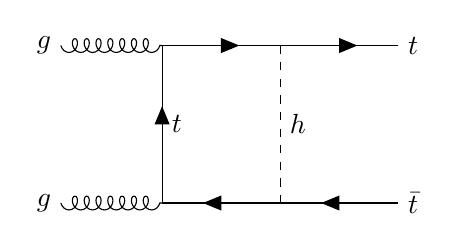
\begin{tikzpicture}
      \begin{feynman}
        \vertex (i1) {\(g\)};
        \vertex [below=2.0 cm of i1] (i2) {\(g\)};
        \vertex [right=1.5 cm of i1] (a);
        \vertex [right=1.5 cm of i2] (b);
        \vertex [right=1.5 cm of a] (c);
        \vertex [right=1.5 cm of b] (d);
        \vertex [right=1.5 cm of c] (f1) {\(t\)};
        \vertex [right=1.5 cm of d] (f2) {\(\bar{t}\)};
        \diagram* {
          (i1) -- [gluon] (a),
          (i2) -- [gluon] (b),
          (c) -- [scalar, edge label=\(h\)] (d),
          (f1) -- [anti fermion] (c) -- [anti fermion] (a) -- [anti fermion, edge label=\(t\)] (b) -- [anti fermion] (d) -- [anti fermion] (f2)
        };
      \end{feynman}
    \end{tikzpicture}
    \caption{\textbf{EW correction involving a SM Higgs boson.} An example Feynman diagram for NLO EW corrections to \ttbar production involving the exchange of a virtual SM Higgs boson $h$.}
    \label{fig:ah:ewcorr_feynman}
\end{figure}

The NLO corrections in the electroweak coupling \alphaew are computed with the HATHOR code~\cite{Aliev:2010zk, Kuhn:2005it, Kuhn:2006vh, Kuhn:2013zoa} using a dynamic scale choice of $\mu_R = \mu_F = \frac{1}{2} \mtt$. Of particular interest here is a class of diagrams which contain an exchange of a virtual SM Higgs boson, an example of which is seen in \cref{fig:ah:ewcorr_feynman}. The matrix element for this diagram is proportional to the square of the SM Higgs-top Yukawa coupling \yt, giving a $\yt^2$-dependent correction to \ttbar distributions from the interference with LO diagrams. This correction is sizable mostly for low \mtt values, and is important for this analysis because the SM Higgs exchange might change the \ttbar spin state and thus \chel and \chan. To accurately account for this, the correction is derived separately for the different initial states ($gg$, $q\bar{q}$ and $gq$) of \ttbar production.

The results obtained with HATHOR are accurate only to LO in \alphas, i.e. \order{\alphas^2}, and as of the time of writing no full calculation including both NLO QCD and EW effects exists. Thus, there is an ambiguity on how the NLO-accurate (in QCD) MC simulation and the NNLO-accurate corrections presented in the previous section should be combined with the EW corrections.

Formally, the differential cross section as predicted by Powheg can be decomposed as

\begin{equation}
    d \sigma_{\powheg} = \alphas^2 d \sigma_{\mathrm{LO}} + \alphas^3 d \sigma_{\mathrm{NLO}}
\end{equation}

\noindent where additional terms beyond $\order{\alphas^3}$ due to additional radiation in Powheg and Pythia are not written for simplicity. On the other hand, HATHOR predicts

\begin{equation}
    d \sigma_{\mathrm{HATHOR}} = \alphas^2 d \sigma_{\mathrm{LO}} + \alphas^2 \alphaew d \sigma_{\mathrm{EW}}.
\end{equation}

One possible way to combine the calculations is the additive scheme, given by


\begin{equation}
\begin{split}
\label{eq:ah:ewadd}
    d \sigma_{\mathrm{add.}} &= d \sigma_{\powheg} + d \sigma_{\mathrm{HATHOR}} - \alphas^2 d \sigma_{\mathrm{LO}} \\
    &= \alphas^2 d \sigma_{\mathrm{LO}} + \alphas^3 d \sigma_{\mathrm{NLO}} + \alphas^2 \alphaew d \sigma_{\mathrm{EW}}
\end{split}
\end{equation}

\noindent which is formally accurate to $\order{\alphas^3}$ and $\order{\alphas^2 \alphaew}$. This approach does not include any cross terms of order $\order{\alphas^3 \alphaew}$, which are not fully calculated by either Powheg or HATHOR. However, it is reasonable to assume that these cross terms factorize approximately, leading to the alternative multiplicative scheme~\cite{Kuhn:2013zoa}

\begin{equation}
\begin{split}
\label{eq:ah:ewmult}
    d \sigma_{\mathrm{mult.}} &= d \sigma_{\powheg} \times \frac{d \sigma_{\mathrm{HATHOR}}} {\alphas^2 d \sigma_{\mathrm{LO}}} \\
    &= \alphas^2 d \sigma_{\mathrm{LO}} + \alphas^3 d \sigma_{\mathrm{NLO}} + \alphas^2 \alphaew d \sigma_{\mathrm{EW}} + \alphas^3 \alphaew \frac {d \sigma_{\mathrm{NLO}} \, d \sigma_{\mathrm{EW}}}{d \sigma_{\mathrm{LO}}}
\end{split}
\end{equation}

The difference between the two schemes is in the last term of order $\order{\alphas^3\alphaew}$, which is an approximation to the QCD-EW cross terms. In this work, the multiplicative approach is used for all nominal results, while the difference to the additive approach is included as a systematic uncertainty. In both cases, the needed term $\alphas^2 d \sigma_{\mathrm{LO}}$ is computed with \amcatnlo.

\begin{figure}[t]
    \centering
    \includegraphics[width=0.49\linewidth]{figures/ah/ewqcdcorrs_yt_mtt.pdf}
    \hfill
    \includegraphics[width=0.49\linewidth]{figures/ah/ewqcdcorrs_yt_chel.pdf}
    \caption{\textbf{Effect of \yt variations} in the NLO EW corrections for inclusive \mtt (left) and \chel for $\mtt < \SI{400}{\GeV}$ (right), shown as the ratio to the nominal distributions ($\yt = 1.0$) for detector-level reconstructed observables.}
    \label{fig:ah:yt_variation}
\end{figure}

The effect of both approaches on the 3D \mttchelchan distribution at the detector level after parton showering can be seen in \cref{fig:ah:ewqcdcorrs}. The multiplicative scheme leads to a larger correction of roughly $2-4\%$, while the additive scheme only gives $1-2\%$. 

Furthermore, the effect of varying \yt modifies not only the \mtt distribution close to the \ttbar threshold, but also the distribution of \chel. This is shown again more explicitly in \cref{fig:ah:yt_variation} for the one-dimensional \mtt and \chel distributions. As a result, such a variation in data could potentially be confused for a pseudoscalar signal. It is thus important to include it as a systematic uncertainty, as described in \cref{sec:ah:systs}.


\section{Matrix element reweighting for \AH signals}
\label{sec:ah:mereweighting}

In order to probe the full phase space of the generic \AH model as described in \cref{sec:ah:intro}, predictions at different \AH masses and widths with a sufficiently small spacing are required so that interpolation between the points is possible. However, generating a separate MC sample for each mass and width point is computationally very expensive.

\subsection{Principle of the method}

As an alternative, it is possible to re-use existing samples for different mass and width points via matrix element reweighting. This method works by noting that a given MC sample can be seen as a random sample, drawn from a probability distribution of the form

\begin{equation}
\label{eq:ah:merewprob}
    \mathcal{P}(x_i^{\mathrm{ME}}, x_j^{\mathrm{reco}}) = \mathcal{P}^{\mathrm{ME}} (x_i^{\mathrm{ME}}) \cdot \mathcal{P}^{\mathrm{rem}} (x_j^{\mathrm{reco}} | x_i^{\mathrm{ME}})
\end{equation}

Here, $x_i^{\mathrm{ME}}$ are all variables defining the event at the matrix element (ME) level, i.e. at the level of the hard interaction, and $x_j^{\mathrm{reco}}$ are all variables after detector simulation and object reconstruction. For the case of the \AH signals, which are generated at LO in QCD, $x_i^{\mathrm{ME}}$ is given by the four-momenta and helicities of the final-state particles (leptons, neutrinos and b quarks) in the hard process. The $x_j^{\mathrm{reco}}$ consist of all possible reconstruction-level variables that are relevant to the analysis, such as e.g. jet and lepton four-momenta, lepton identification criteria or \ptmissvec. 

$\mathcal{P}^{\mathrm{ME}} (x_i^{\mathrm{ME}})$ refers to the probability density of the ME-level variables as predicted by the ME generator, which will be proportional to the absolute square of the matrix element. This function will depend on the chosen scenario of the \AH model, i.e. $m_{\AH}$ and $\Gamma_{\AH}$. Meanwhile, the conditional probability density $\mathcal{P}^{\mathrm{rem}} (x_j^{\mathrm{reco}} | x_i^{\mathrm{ME}})$ encodes the effects of all other components of the simulation chain, such as the parton shower, hadronization, detector simulation and reconstruction. It gives the probability to observe reconstruction-level variables $x_j^{\mathrm{reco}}$ for an event with ME-level variables $x_i^{\mathrm{ME}}$.

The principal assumption of the method is now that $\mathcal{P}^{\mathrm{rem}}$, and thus the whole simulation chain except for the matrix element, is independent of the underlying \AH signal scenario ($m_{\AH}$ and $\Gamma_{\AH}$). This assumption is certainly true for the detector simulation and reconstruction, while care must be taken for the parton shower, which in general needs to be matched to the matrix element and can this way have a residual dependence. The validity of the assumption will be discussed in more detail below.

If the assumption is fulfilled, a given \AH MC sample generated with parameters $m_{\AH}^0$ and $\Gamma_{\AH}^0$ can now be reweighted to a different \AH scenario with parameters $\hat{m}_{\AH}$ and $\hat{\Gamma}_{\AH}$ by applying to each event $i$ a weight 

\begin{equation}
\label{eq:ah:merewweight}
    w_i = \frac{ \mathcal{P}^{\mathrm{ME}} (x_i^{\mathrm{ME}} | \hat{m}_{\AH} , \hat{\Gamma}_{\AH} ) } { \mathcal{P}^{\mathrm{ME}} (x_i^{\mathrm{ME}} | m_{\AH}^0 , \Gamma_{\AH}^0 ) }
\end{equation}

The quantities in the denominator and nominator are the ME-level probability densities for each event, evaluated at the original and target \AH parameters, respectively. When this weight is inserted into \cref{eq:ah:merewprob}, the original probability cancels, giving the correct probability density for the target scenario $\hat{m}_{\AH}$ and $\hat{\Gamma}_{\AH}$.

In practice, this method will only work if the MC sample used for the reweighting has sufficient phase space overlap with the target \AH scenario, i.e. if the two probabilities in \cref{eq:ah:merewweight} are not too different from each other for the majority of the events. Otherwise, the weights will become very small in some regions of the phase space and very large in others, resulting in poor statistics for the reweighted sample.

The method was implemented by directly evaluating the squared matrix elements for the different \AH hypotheses, using the standalone reweighting interface provided by \amcatnlo and the same UFO model as for the signal generation. 

\subsection{Combination of multiple origin samples}

At the time of this analysis, a set of signal samples for different \AH scenarios (as given in \cref{sec:ah:datasets}) was already available. These samples were used as origin samples for the reweighting. To maximize the statistical power of the method and to mitigate problems from poor phase space overlap, subsets of the available samples were combined during reweighting and ranked with an average event weight.

In detail, this procedure works as follows: First, a set of several samples $j$ (the origin samples) with different parameters $m_{\AH}$ and $\Gamma_{\AH}$ are all reweighted separately to the same target parameters $\hat{m}_{\AH}$ and $\hat{\Gamma}_{\AH}$ with per-event weights $w_{i,j}$ as given in \cref{eq:ah:merewweight}. These need to be multplied with a possible generator weight of the origin sample $u_{i,j}$, giving the total per-event weight $\hat{w}_{i,j} = w_{i,j} u_{i,j}$. For fully unweighted origin samples, $u_{i,j} = 1$. 

Then, the different samples are weighted with a per-sample weight $v_j$ proportional to

\begin{equation}
\label{eq:ah:sampleweights}
    v_j \propto {\langle \hat{w}_{i,j} \rangle}^{-1} =  \frac{ \sum_i \hat{w}_{i,j} }{ \sum_i \hat{w}_{i,j}^2 }
\end{equation}

\noindent where the sums run over all the events $i$ in the considered sample $j$. This expression is the inverse of the average ME weight for sample $j$. It is chosen such that samples with large phase space overlap with the target \AH scenario - and thus small ME weights $w_{i,j}$ - are assigned a large weight $v_j$ in the combination of samples. Similarly, samples with poor phase space overlap, and thus large average ME weights, get assigned small weights and contribute less strongly to the combined sample. Finally, the total combined sample is normalized to the expected cross section for the target scenario, which is calculated independently. It is shown in App.~\ref{app:mereweighting} that this procedure minimizes the total statistical error of the combined sample.

In practice, all available masses and parities (A and H) are combined for each target \AH mass. Resonance and interference contributions are treated separately from each other. Furthermore, it was found that, for the resonance contribution only, it is necessary to split the combination of different \AH widths into two halves: those with $\wAH/\mAH$ less or greater than 10\%. This is due to an interplay of \amcatnlo and the \pythia shower leading to a dependency on the \AH width in the matrix element, which is not taken into account in the reweighting. For $\wAH/\mAH < 10\%$ (narrow resonance), \amcatnlo includes the intermediate \AH particle in the event record, which is then treated by \pythia as a unstable resonance and its virtuality as predicted by the matrix element is preserved. For $\wAH/\mAH \geq 10\%$ (broad resonance), the \AH particle is not included in the event record, and its virtuality is thus not preserved. This leads to slight differences in distributions affected by the parton showering. The choice of 10\% for the transition between the two modes is an arbitrary parameter, and thus not necessarily physical. Nonetheless, it was decided in this analysis to not mix the two width ranges in the reweighting in order to obtain full closure with a standalone generation.

\subsection{Validation}

The combined reweighting is validated for two masses of $\mAH = 400$ and 800 GeV as well as widths of 2.5 and 10\%. For each of these points, the reweighting is performed as stated above, but leaving out \AH scenarios with the same mass from the combination of origin samples since otherwise the weights would be trivially one. The reweighted \mtt distributions at generator level are then compared to the standalone samples at the same \mAH and \wAH.

The resulting comparisons and residuals can be seen in \cref{fig:ah:merew_validation} for A and H, separated into the resonance and interference contributions. It can be seen that the closure between reweighting and standalone generation is excellent within the statistical uncertainties.

\begin{figure}[!p]
    \centering
    \includegraphics[width=0.49\textwidth]{figures/ah/me_reweighting/A_res.pdf}
    \hfill
    \includegraphics[width=0.49\textwidth]{figures/ah/me_reweighting/H_res.pdf}
    \includegraphics[width=0.49\textwidth]{figures/ah/me_reweighting/A_int.pdf}
    \hfill
    \includegraphics[width=0.49\textwidth]{figures/ah/me_reweighting/H_int.pdf}
    \caption{\textbf{Validation of the ME reweighting.} Comparison of standalone generated (lines) and reweighted (diamond markers) \mtt distributions for different values of \mAH and \wAH. From top left to bottom right: A resonance, H resonance, A interference, H interference. The lower panel shows the difference of reweighted and standalone distributions, normalized to the standalone distributions. The error bars give the combined statistical uncertainty of the reweighted and standalone sample.}
    \label{fig:ah:merew_validation}
\end{figure}

\section{Systematic uncertainties}
\label{sec:ah:systs}

Similar to \cref{sec:ttxs:systematics}, systematic uncertainties affect the distributions of both SM background and signal processes. They are listed in this section, split into theory (\cref{sec:ah:theorysysts}) and experimental uncertainties (\cref{sec:ah:expsysts}).

\subsection{Theory uncertainties}
\label{sec:ah:theorysysts}

\paragraph{Scale uncertainties}
Uncertainties due to missing higher orders in the matrix element as well as the parton shower are included separately for the SM \ttbar, tW, and Z+jets backgrounds as well as all considered signals by varying the associated scales by a factor 2 up and down independently, same as in \cref{sec:ttxs:systematics}. Only the shape components of the ME scales are taken from the respective ME generators, while the normalization uncertainty is treated externally, as described below. For A and H, the uncertainties are considered uncorrelated between the resonance and interference components, which is found to be conservative. For \etat, the renormalization scale uncertainty is not included since the considered model does not encode any dependence on either $\mu_R$ or \alphas.

\paragraph{PDF uncertainties}
For the SM \ttbar background, the uncertainty due to the PDF is again included based on the 100 provided eigenvalues of the NNPDF 3.1 PDF set. However, it is not sufficient to simply take the envelope of these variations since this would capture only the change in \ttbar normalization, while this anaylsis is mostly sensitive to shape variations.

Instead, a principal component analysis (PCA) is performed on the final 3D \mttchelchan templates obtained from the different eigenvalues, thus finding those linear combinations that have a noticeable shape effect. Only the first eigenvector (corresponding to the largest eigenvalue) is non-negligible, and this variation is considered as the PDF uncertainty. For more details on this procedure, see \citere{Rubenach:PhD}. Independently of this, another uncertainty based on the value of \alphas in the PDF is considered similarly to \cref{sec:ttxs:systematics}.

\paragraph{EW correction uncertainties}
As described in \cref{sec:ah:ewcorr}, two independent uncertainties are attached to the NLO electroweak correction of SM {\ttbar}: First, the value of the SM top-Higgs Yukawa coupling is allowed to vary in the range $\yt = {1.00}^{+0.11}_{-0.11}$, with the range given by the uncertainty of the experimental measurement in \citere{CMS:HIG-17-031}. Second, the difference between the additive and multiplicative application scheme (\cref{eq:ah:ewadd,eq:ah:ewmult}) is considered as a separate uncertainty, as recommended in \citere{Kuhn:2013zoa}, and symmetrized around the nominal.

\paragraph{Top quark mass uncertainty}
The top quark mass uncertainty in SM \ttbar is estimated by varying it from its nominal value of $\mt = \SI{172.5}{\GeV}$ by $\pm \SI{3}{\GeV}$ in the \powheg simulation, and then scaling down the resulting relative deviation by a factor $1/3$, leading to a $\pm \SI{1}{\GeV}$ uncertainty. This is done since the variation, obtained from an independent MC sample, is otherwise plagued by large statistical uncertainties. Furthermore, the top mass is also varied in all considered signal samples directly by $\pm \SI{1}{\GeV}$ through an ME reweighting method similar to \cref{sec:ah:mereweighting}. The chosen range of $\pm \SI{1}{\GeV}$ is conservative with respect to the most precise top mass measurements at the time of writing, which have uncertainties on the order of \SI{0.4}{\GeV}~\cite{CMS:TOP-20-008,ATLASCMS:2024dxp}. The top mass uncertainties between background and signals are considered as fully correlated.

\paragraph{Further uncertainties in SM \ttbar}
Additionally, separate SM \ttbar samples are used to evaluate uncertainties due to ME/PS matching (same as in \cref{sec:ttxs:systematics}), the underlying event tune~\cite{CMS:GEN-17-001}, and the color reconnection model in \pythia~\cite{CMS:GEN-17-002,Christiansen:2015yqa}. All of these effects are found to be small.

\paragraph{Background cross section uncertainties}
For the SM \ttbar background, the shift in the predicted NNLO+NNLL \ttbar cross section due to the ME scale variations as well as the top quark mass is calculated with Top++~\cite{Czakon:2011xx} in the same manner as the nominal cross section. The resulting shifts in the cross section are ${}^{+20.5}_{-17.9}\,\si{\pb}$ for a variation of $\mu_F$ by a factor two up and down, ${}^{-30.1}_{+9.6}\,\si{\pb}$ for a similar variation of $\mu_R$, and ${}^{-22.5}_{+23.5}\,\si{\pb}$ for a top mass variation in the range $\pm \SI{1}{\GeV}$. These three variations are treated as fully correlated with the respective shape uncertainties obtained at NLO from the \powheg simulation as described above, so that no additional nuisance parameter for the \ttbar normalization is introduced.

For minor backgrounds, explicit uncertainties of 15\% for tW and t-channel single top~\cite{ATLAS:2016ymp,CMS:TOP-17-011,CMS:TOP-17-018}, 30\% for diboson and \ttbar+X~\cite{CMS:TOP-17-005,ATLAS:2019njj}, and 5\% for the data-driven \Zgamma+jets normalization~\cite{ATLAS:2016oxs} are considered, which are all based on the precision of relevant cross section measurements.

\paragraph{Background statistical uncertainties}
Again similar to \cref{sec:ttxs:systematics}, per-bin background statistical uncertainties for all simulated processes are included following \citere{Barlow:1993dm}.

\subsection{Experimental uncertainties}
\label{sec:ah:expsysts}

\paragraph{Jet and \ptmiss uncertainties}
The uncertainty on the calibration of the jet \pt detector response is assessed through the ``reduced'' set of subsources provided by the CMS Collaboration, which encompasses seven different subsources. Of these, five subsources are found to be relevant for this analysis, while two subsources affecting mainly the endcaps and hadronic forward calorimeter are negligible. The five relevant subsources are:

\begin{itemize}
    \item The absolute scale uncertainty,  referring to the constant term in the jet \pt response (``\texttt{Absolute}''). It is split into a statistical component (uncorrelated between years) and a systematic component (correlated), the latter encoding e.g. corrections due to FSR and ISR in the JEC derivation.
    \item The relative scale uncertainty in the barrel and first part of the endcaps ($\abseta < 2.5$), encoding the \pt dependence of the jet \pt response (``\texttt{BBEC1}''). It is similarly split into an uncorrelated statistical and a correlated systematic component.
    \item An uncertainty due to residual differences in the $\eta$ dependence between JECs derived in dijet, Z+jets, and $\gamma$+jets selections (``\texttt{RelativeSample}''), considered uncorrelated between years.
    \item An uncertainty due to residual differences between different methods of deriving the JECs (``\texttt{RelativeBal}''), considered fully correlated between years.
    \item An uncertainty due to the difference in jet flavor response in \pythia and \herwig, considered separately for b quark jets (``\texttt{FlavorPureBottom}'') and non-b quark jets (``\texttt{FlavorQCD}'') and fully correlated between years.
\end{itemize}

Furthermore, the uncertainty in the jet \pt resolution is considered separately, again uncorrelated between years. All jet uncertainties are fully propagated to the calculation of \ptmiss, and an additional \ptmiss uncertainty based on soft, unclustered hadronic activity is also considered.

\paragraph{b tagging uncertainties}
Similarly, the uncertainty on the b tagging efficiency is split into 17 subsources, corresponding e.g. to different parton shower modeling, the treatment of leptons in the jet, or the propagation of the jet \pt scale uncertainties~\cite{CMS:BTV-16-002}. One component represents the statistical uncertainty and is thus considered uncorrelated, while all others are correlated among years. Moreover, an uncertainty on mistagging of light-flavor jets is included, also split into a statistical and a systematic component.

\paragraph{Lepton and trigger uncertainties}
Uncertainties on the lepton reconstruction, identification, and isolation efficiencies, as measured centrally in CMS using the tag-and-probe method, are considered separately for muons and electrons~\cite{CMS:EGM-17-001,CMS:MUO-16-001}. For the muons, the uncertainty is split into a statistical component (uncorrelated between the analysis years) and a systematic component (correlated), which is based on e.g. the requirements applied to the tag muon or the choice of function used for the tag-and-probe fit. Similarly, the dilepton trigger efficiency uncertainties are considered uncorrelated between years and lepton flavor channels. Finally, in data taken in 2016 or 2017, an additional uncertainty is assigned due to an inefficiency in the ECAL L1 trigger~\cite{CMS:TRG-17-001}, as described in \cref{sec:ah:expcorrs}.

\paragraph{Luminosity uncertainty}
The uncertainty on the total integrated luminosity is included following \citeres{CMS:LUM-17-003,CMS:LUM-17-004,CMS:LUM-18-002}, leading to a total luminosity uncertainty of $1.6\%$, split into a total of seven components that encode the correlations between the years. Similar as in \cref{sec:ttxs:systematics}, the largest single contributions to the uncertainty come from factorization between the $x$ and $y$ axes during scans used for the luminosity calibration as well as due to residual differences between different luminosity detectors~\cite{CMS:LUM-17-003}. 

\paragraph{Pileup uncertainty}
To estimate the uncertainty on the amount of pileup per pp bunch crossing, the effective inelastic proton-proton cross section used for pileup reweighting in the simulation is varied by 4.6\% from its nominal value~\cite{CMS:FSQ-15-005}.

\subsection{Uncertainty smoothing}
Several of the considered uncertainty sources, e.g. the top quark mass in SM \ttbar, are estimated by comparing to separate MC samples, which causes the relative deviation due to the source to be affected by large statistical noise. A similar problem appears for uncertainties which effectively vary the cuts applied on MC events, such as e.g. the jet \pt scale uncertainties by way of jet acceptances. If left untreated, fitting these noisy shape templates to the data could lead to erroneous constraints in the likelihood fit. 

To prevent this, a smoothing procedure based on the algorithm LOWESS (short for \textit{locally weighted scatterplot smoothing})~\cite{Cleveland:1979,Cleveland:1988} is applied to these sources. The procedure follows \citere{Anuar:PhD} and is described briefly in the following. First, the relative deviation of the respective source is defined as $r^\pm = (N^\pm - N^0) / N^0$, where $N^0$, $N^+$, and $N^-$ are the event yields for the nominal template, the up variation, and the down variation. They are considered three-dimensionally (3D) as a function of the sensitive observables $\vec{x} = (\mtt, \, \chel, \, \chan)$. To avoid artifacts from the choice of binning in the analysis, the number of bins along each direction of $\vec{x}$ is doubled for the purpose of the smoothing.

Second, for each bin in $\vec{x}$, a 3D hyperplane is fitted to $r^\pm$ using a least-squares fit. The fit is performed in a 3D \textit{sliding window} with a fixed size of $2 h_i$ in each direction, where $h_i$ with $i = 1,2,3$ is the \textit{bandwidth} along each axis. This means that only bins close to the bin that is being evaluated enter in the fit. Furthermore, the bins enter the fit with a weight depending on their distance to the bin being evaluated. If $\vec{x}$ denotes the bin being evaluated, the weight of bin $\vec{y}$ is given by~\cite{Anuar:PhD}

\begin{equation}
    w (\vec{x}, \vec{y}) = \left( 1 - d(\vec{x}, \vec{y})^3 \right)^3, \quad d(\vec{x}, \vec{y}) = \sqrt{ \sum_i \left( \frac{x_i - y_i}{2 h_i} \right)^2 } .
\end{equation}

The function $w (\vec{x}, \vec{y})$ equals 1 for $\vec{x} = \vec{y}$, i.e. each bin enters with maximal weight 1 in its own fit, and falls off to 0 when $\vec{y}$ tends towards the edge of the sliding window as given by $h_i$. This local weighting thus favors points close to the bin being evaulated.

\begin{figure}[!t]
    \centering
    \includegraphics[width=0.99\textwidth]{figures/ah/smoothing_example.pdf}
    \caption{
        \textbf{Uncertainty smoothing.} The smoothed (solid lines) and unsmoothed (diamond markers) relative deviations in \mttchelchan, shown for the example of the JEC subsource encoding the flavor response of non-b quark jets. The MC statistical uncertainty of the nominal sample is shown in grey. 
    }
    \label{fig:ah:smoothing}
\end{figure}


The bandwidths $h_i$ are free parameters of the method and are chosen using \textit{leave-one-out cross validation} for each uncertainty source separately. In this method, the events making up the templates are randomly split into 10 batches, and nine of these batches are combined into the \textit{training set} while the last is considered the \textit{testing set}. The smoothing is applied to the relative deviation as computed from the training set, where the three bandwiths are scanned in fixed grids given by $h_i \in (0.1, 0.2, 0.5, 0.7, 1.0)$ for \mtt and $h_i \in (0.33, 0.50, 0.83, 1.0)$ for \chel and \chan, all understood as relative to the total bin range in the respective axis. The resulting smoothed template is compared to the unsmoothed template in the testing set, and a $\chi^2$ is computed taking into account the statistical uncertainty of the testing set. This procedure is repeated with each of the ten batches as the testing set, and it is further repeated 50 times with different random partitions. For each choice of bandwidths, the average $\chi^2$ from all repetitions is computed, and the set of bandwidths which minimizes the average $\chi^2$ is chosen for the smoothing.

To further prevent the algorithm from erroneously interpreting statistical noise as shape information, each relative deviation is also fitted using a constant line. The $\chi^2$ is again calculated, and if it is found to be smaller than the $\chi^2$ obtained from the smoothing, the uncertainty source in question is replaced by a pure normalization uncertainty as given by the constant line fit. In practice, this is relevant for some of the minor backgrounds as well as the signals due to the small statisics of their samples, but never occurs for the SM \ttbar background.

The results of the smoothing for the optimal bandwidth are shown for the example of the JEC subsource encoding the flavor response of non-b quark jets (the largest of the JEC subsources) in \cref{fig:ah:smoothing}. The noise visible in the unsmoothed distributions is fully mitigated by the smoothing procedure.


%To prevent this, the smoothing algorithm LOWESS~\cite{Cleveland:1979,Cleveland:1988} is applied to the relative deviations for these sources, with the bandwidth used for the smoothing determined separately through cross-validation for each source. For more details on the procedure, see \citere{Anuar:PhD}.

\subsection{Differences between MC generators}
\label{sec:ah:gennps}

It has been observed that the theoretical uncertainties collected in \cref{sec:ah:theorysysts} do not necessarily cover the differences in the predictions of different MC generators for \ttbar~\cite{ATLAS:2018ivx,CMS:TOP-17-002,CMS:TOP-23-001,ATLAS:2023fsd}. To assess the size of these effects, the standard \ttbar prediction, as computed using \powheg in the NWA matched to \pythia (cf. \cref{sec:mc:ttbar}), is compared to alternate generator setups.%, namely:

%\begin{itemize}
%    \item \powheg \hvq matched to \herwig;
%    \item \amcatnlo matched to \pythia;
%    \item \powheg \bbfourl matched to \pythia.
%\end{itemize}

The first of these is the same \powheg matrix element in the NWA (using the \hvq subprocess in \powheg) matched to the multi-purpose event generator \herwig instead of \pythia. The angular-ordered parton shower in \herwig is used (as opposed to the \pt-ordered dipole shower in \pythia) together with the CMS CH3 tune~\cite{CMS:GEN-19-001}. Furthermore, \herwig uses a cluster hadronization model~\cite{Webber:1983if} instead of the string hadronization model of \pythia as described in \cref{sec:mc:hadronization}.

\begin{figure}[!t]
    \centering
    \includegraphics[width=0.32\textwidth]{figures/ah/altbgs/generators_mtt_cms.pdf}
    \hfill
    \includegraphics[width=0.32\textwidth]{figures/ah/altbgs/generators_chel_lowmtt_cms.pdf}
    \hfill
    \includegraphics[width=0.32\textwidth]{figures/ah/altbgs/generators_chel_highmtt_cms.pdf}
    \caption{
        \textbf{Comparison between MC generators for \tttWsum.} The predictions of different MC setups, namely \powheg \tttWsum matched to \herwig (grey), \bbfourl matched to \pythia (orange), and \amcatnlo matched to \pythia (blue), all shown as the ratio to the prediction of \powheg \tttWsum matched to \pythia, for the inclusive reconstructed \mtt distribution (left) as well as the reconstructed \chel distribution, restricted to $\mtt < \SI{360}{\GeV}$ (center) and to $600 < \mtt < \SI{800}{\GeV}$ (right). The effect of the \etat signal is also shown in red for comparison~\cite{CMS:TOP-24-007}.
    }
    \label{fig:ah:herwigbb4l}
\end{figure}

\Cref{fig:ah:herwigbb4l} shows the ratios of the predictions from \herwig and \pythia for the reconstructed \mtt distribution, as well as for the \chel distribution close to the \ttbar threshold (i.e. where the \etat signal is located) and in the \ttbar continuum. Besides a significantly lower \ttbar acceptance, \herwig predicts an increase of events at the \ttbar threshold similar to \etat.
This appears concerning at first glance since, should the data follow the prediction from \herwig instead of \pythia, this enhancement could be confused with an \etat signal if \pythia is used as the baseline prediction.
However, as seen in \cref{fig:ah:herwigbb4l} in the center, \herwig at the same predicts a flatter slope in \chel than \pythia at the \ttbar threshold, equivalent to a reduction of \ttbar spin correlations\footnote{This effect was also seen in the context of \citere{ATLAS:2023fsd}.}. This is in contrast to the \etat signal, in which the \ttbar spins are maximally anti-correlated. The inclusion of the spin correlation variable \chel in the analysis thus ensures that a possible signal cannot be faked if the data follow the \herwig instead of the \pythia prediction.
%makes it possible to separate the differences between \powheg and \herwig with respect to \etat.

The second alternative generator is \bbfourl matched to \pythia, as studied extensively in \cref{ch:bb4l}. Here, particularly the off-shell effects included in \bbfourl might be of interest for the extraction of \etat since the latter is located below the \ttbar threshold. The setup denoted as ``\bbfourl v2'' in \cref{sec:bb4l:bb4l}, corresponding to \citere{Jezo:2023rht}, is used, and compared to the sum of the NWA-based \powheg \ttbar and tW predictions for consistency exactly like in \cref{sec:bb4l:tttW}.

A caveat here is presented by the corrections to NNLO QCD and NLO EW as described in \cref{sec:ah:ttbarweights}. These are derived from fixed-order corrections assuming stable top quarks, and are not available for the full \bbllnunu final state. To still be able to apply them to \bbfourl predictions, the \bbfourl sample is split into a \ttbar and a tW part in an ad-hoc way by using the matrix element history projectors implemented in \bbfourl~v2~\cite{Jezo:2023rht}. The corrections are then applied to the \ttbar part only, in the same manner as to the NWA-based \powheg \ttbar sample.

%\begin{figure}[!t]
%    \centering
%    \includegraphics[width=0.49\textwidth]{figures/ah/altbgs/hvqvsbb4l_mtt.pdf}
%    \hfill
%    \includegraphics[width=0.49\textwidth]{figures/ah/altbgs/hvqvsbb4l_chel_lowmtt.pdf}
%    \caption{
%        \textbf{Comparison of \powheg \tttWsum and \bbfourl.} The ratio of the predictions of the sum of \powheg \hvq \ttbar and tW to \bbfourl (all matched to \pythia) for the inclusive reconstructed \mtt distribution (left) and the reconstructed \chel distribution, restricted to $\mtt < \SI{360}{\GeV}$ (right). The effect of the \etat signal is also shown for comparison.
%    }
%    \label{fig:ah:bb4l}
%\end{figure}

The ratios of the predictions are also shown in \cref{fig:ah:herwigbb4l}. It can be seen that \bbfourl does not predict major differences in the reconstructed \mtt spectrum (left) even at its lower edge. However, it results in a significantly steeper slope in reconstructed \chel close to the threshold (center). This increase in slope is of similar magnitude as the effect expected due to \etat. 

The source of this difference is not yet fully understood. \bbfourl contains NLO QCD corrections to the top decay which are not present in the NWA-based \ttbar sample (though they are approximated through the matrix element corrections in \pythia). However, NLO corrections to spin correlations are expected to be only on the percent level and to reduce the spin correlation instead of enhancing it~\cite{Bernreuther:2004jv}. 

It is possible that the effect instead originates in the \tttW interference:
%The tW contribution on its own is expected to have close to flat \chel since one of the leptons is not actually the decay product of a top quark, and the interference between \ttbar and tW is destructive in large parts of the phase space. If the interference in \bbfourl is now larger than in \tttWsum, it could thus reduce the contribution from tW, effectively enhancing the \chel slope. 
For the tW contribution, where one of the leptons is not actually the decay product of a top quark,
\chel does not analyze spin correlation, since there is only one (anti-)top involved in the process. 
%\ttbar spin correlation is not truly definable.
Therefore, the slope of the reconstructed \chel distribution under the SM prediction for tW is not related to \ttbar spin correlation and thus in general different to the slope in SM \ttbar. The same holds for the \tttW interference. Since \bbfourl now gives a true prediction of the \tttW interference instead of the ad-hoc treatment of the DR and DS schemes (cf. \cref{sec:bb4l:others}), it is expected that the magnitude of the interference contribution in \bbfourl will be different. Thus, it is possible that the total \chel slope, arising from the combination of \ttbar, tW, and \tttW interference, will be different as well.
%However, since \ttbar and tW are not cleanly separable in \bbfourl, however, this hypothesis is difficult to confirm, and such studies are beyond the scope of this analysis.

%For the purpose of the \etat extraction, the differences to these alternative generator setups are included in the fit as two additional shape-based nuisance parameters (one for \pythia compared to \herwig, and one for \tttWsum compared to \bbfourl). In both cases, the \powheg \hvq + \pythia prediction is considered the nominal, and the alternate prediction is considered the $+1\sigma$ template. The $-1\sigma$ template is constructed by symmetrizing the relative difference around the nominal, and intermediate values are obtained by interpolation as usual. \todo{where are the NPs used and where not}

A third alternative prediction is provided by \ttbar+jets production simulated with \amcatnlo, matched to \pythia with the FxFx scheme~\cite{Frederix:2012ps}. While this prediction is formally also NLO-accurate in QCD in the NWA, and thus comparable to the NWA-based \powheg prediction, it has been observed in past measurements that \amcatnlo does not agree as well with data as \powheg for \ttbar production. Indeed it shows a large slope in the \mtt distribution, as also seen in \cref{fig:ah:herwigbb4l}. As a result, \amcatnlo is given less focus compared to the other two predictions here.

At high values of \mtt, the slope of \chel is consistent between all considered generators, as shown in \cref{fig:ah:herwigbb4l} (right). Only normalization differences due to acceptance as well as the shape differences in \mtt remain. This shows that the modeling of spin correlations in the bulk of the \mtt distribution is reliable and should be considered uncontroversial.

In this work, NWA-based \ttbar using \powheg + \pythia is considered for the nominal background prediction in all cases. A comparison to \powheg + \herwig, \amcatnlo + \pythia, and \bbfourl + \pythia is shown in \cref{sec:ah:checks} in the context of measuring the \etat cross section. Furthermore, the effect of including the differences to \powheg + \herwig and \bbfourl + \pythia as two additional shape-based nuisance parameters in the fit is similarly given in \cref{sec:ah:checks}. Note that in \citere{CMS:TOP-24-007}, these nuisance parameters were considered as part of the main result in order to be conservative with respect to the total uncertainty.

\section{Pre-fit distributions}
\label{sec:ah:prefit}

\begin{figure}[!hp]
    \centering
    \includegraphics[width=0.49\textwidth]{figures/ah/controlplots/ReqMET/lep_pt__sf.pdf}
    \hfill
    \includegraphics[width=0.49\textwidth]{figures/ah/controlplots/ReqMET/lep_pt__em.pdf}
    \includegraphics[width=0.49\textwidth]{figures/ah/controlplots/ReqMET/lep_eta__sf.pdf}
    \hfill
    \includegraphics[width=0.49\textwidth]{figures/ah/controlplots/ReqMET/lep_eta__em.pdf}
    \includegraphics[width=0.49\textwidth]{figures/ah/controlplots/ReqMET/lep_deltaphi__sf.pdf}
    \hfill
    \includegraphics[width=0.49\textwidth]{figures/ah/controlplots/ReqMET/lep_deltaphi__em.pdf}
    \caption{
        \textbf{Control distributions.} Shown are the distributions of \pt of both leptons (top), $\eta$ of both leptons (center), and the azimuthal angle \dphill between the leptons (bottom) in the combined \ee/\mumu channels (left) and the \emu channel (right). All figures show both data (black dots) and different simulated background processes (colored bars), as well as the total systematic uncertainty (gray band). 
    }
    \label{fig:ah:control1}
\end{figure}

\begin{figure}[!hp]
    \centering
    \includegraphics[width=0.49\textwidth]{figures/ah/controlplots/ReqMET/jet_pt__sf.pdf}
    \hfill
    \includegraphics[width=0.49\textwidth]{figures/ah/controlplots/ReqMET/jet_pt__em.pdf}
    \includegraphics[width=0.49\textwidth]{figures/ah/controlplots/ReqMET/jet_eta__sf.pdf}
    \hfill
    \includegraphics[width=0.49\textwidth]{figures/ah/controlplots/ReqMET/jet_eta__em.pdf}
    \includegraphics[width=0.49\textwidth]{figures/ah/controlplots/ReqMET/njet__sf.pdf}
    \hfill
    \includegraphics[width=0.49\textwidth]{figures/ah/controlplots/ReqMET/njet__em.pdf}
    \caption{
        \textbf{Control distributions.} Shown are the distributions of \pt of all jets (top), $\eta$ of all jets (center), and the number of jets (bottom) in the combined \ee/\mumu channels (left) and the \emu channel (right). All figures show both data (black dots) and different simulated background processes (colored bars), as well as the total systematic uncertainty (gray band). 
    }
    \label{fig:ah:control2}
\end{figure}

\begin{figure}[!hp]
    \centering
    \includegraphics[width=0.49\textwidth]{figures/ah/controlplots/ReqMET/METpt__sf.pdf}
    \hfill
    \includegraphics[width=0.49\textwidth]{figures/ah/controlplots/ReqMET/METpt__em.pdf}
    \includegraphics[width=0.49\textwidth]{figures/ah/controlplots/ReqMET/mll__sf.pdf}
    \hfill
    \includegraphics[width=0.49\textwidth]{figures/ah/controlplots/ReqMET/mll__em.pdf}
    \includegraphics[width=0.49\textwidth]{figures/ah/controlplots/ReqMET/mbbll__sf.pdf}
    \hfill
    \includegraphics[width=0.49\textwidth]{figures/ah/controlplots/ReqMET/mbbll__em.pdf}
    \caption{
        \textbf{Control distributions.} Shown are the distributions of \ptmiss (top), \mll (center), and the invariant mass \mbbll of both b candidates and both leptons (bottom) in the combined \ee/\mumu channels (left) and the \emu channel (right). All figures show both data (black dots) and different simulated background processes (colored bars), as well as the total systematic uncertainty (gray band). 
    }
    \label{fig:ah:control3}
\end{figure}

\begin{figure}[!hp]
    \centering
    \includegraphics[width=0.49\textwidth]{figures/ah/controlplots/Reco/top_pt__ll.pdf}
    \hfill
    \includegraphics[width=0.49\textwidth]{figures/ah/controlplots/Reco/top_eta__ll.pdf}
    \includegraphics[width=0.49\textwidth]{figures/ah/controlplots/Reco/costhetastar__ll.pdf}
    \hfill
    \includegraphics[width=0.49\textwidth]{figures/ah/controlplots/Reco/mtt__ll.pdf}
    \includegraphics[width=0.49\textwidth]{figures/ah/controlplots/Reco/chel__ll.pdf}
    \hfill
    \includegraphics[width=0.49\textwidth]{figures/ah/controlplots/Reco/chan__ll.pdf}
    \caption{
        \textbf{Control distributions after \ttbar reconstruction.} Shown are (from top left to bottom right) the distributions of the top quark \pt, top quark $\eta$, \mtt, \cost, \chel and \chan for the combined dilepton channels. All figures show both data (black dots) and different simulated background processes (colored bars), as well as the total systematic uncertainty (gray band). 
    }
    \label{fig:ah:controlttbar}
\end{figure}

The agreement between the total MC prediction, including all corrections described in \cref{sec:ah:expcorrs,sec:ah:ttbarweights}, and the observed data are presented in this section. Shown observables are lepton \pt, $\eta$, and \dphill (\cref{fig:ah:control1}); jet \pt, $\eta$, and number of jets (\cref{fig:ah:control2}); as well as \ptmiss, the invariant mass of the two leptons \mll, and the invariant mass of the two leptons and two b tagged jets \mbbll (\cref{fig:ah:control3}). All of them are shown after all lepton, jet, b tag and \ptmiss requirements, but before the \ttbar reconstruction, summed over all analysis years, and separately for the same-flavor (\ee and \mumu) and opposite-flavor (\emu) channels, since the latter have different backgrounds and cuts.

Furthermore, different distributions resulting from the \ttbar reconstruction are shown in \cref{fig:ah:controlttbar} for all three channels combined. They consist of top quark \pt, $\eta$, and scattering angle \cost, as well as the three observables used for the fit \mtt, \chel, and \chan.

It can be seen that there is a slight but consistent over-prediction of the background normalization compared to the data in almost all distributions, which could be due to a small misestimation of the acceptance. Alternatively, it could originate from the NNLO+NNLL \ttbar cross section used to normalize the sample; inclusive cross section measurements have consistently shown a slightly lower cross section in data compared to this prediction (cf. \cref{fig:ttxs:ttcurve}). Since this analysis is mostly sensitive to shape effects, and the normalization difference is covered by the uncertainties, this is unproblematic in this context.

Furthermore, there is a slight slope in the ratio of data and simulation yields in the \pt of leptons, jets or the reconstructed top quarks. This is likely a result of the well-known top quark \pt mismodeling at the LHC, which is not fully removed by NNLO QCD corrections as used here~\cite{CMS:TOP-16-008,CMS:TOP-17-014}. It is fully covered by the matrix element scale uncertainties, which are evaluated at NLO as discussed in \cref{sec:ah:theorysysts}. A related discrepancy is seen for high values of \abseta and is similarly covered. Moreover, there is a small discrepancy for large number of jets, which is fully covered by matrix element and parton shower scale systematics (cf. \cref{sec:ah:theorysysts}). In total, all distributions show agreement within the statistical and systematic uncertainties.

Finally, the three-dimensional \mttchelchan distribution used for the statistical analysis is shown before the fit, including all systematic uncertainties, in \cref{fig:ah:prefit_ll}. A notable excess of the data compared to the prediction is observed for low values of \mtt, consistent with the excess seen in the one-dimensional \mtt distribution (\cref{fig:ah:controlttbar}) and in the related observables \mll and \mbbll (\cref{fig:ah:control3}). The excess is stronger for large values of \chel as seen from the multi-dimensional binning, while no trend can be seen by eye regarding \chan.

\begin{figure}[t]
    \centering
    \includegraphics[width=0.99\textwidth]{figures/ah/prepost/A_m365_w2p0__H_m365_w2p0_fit_p_ll_run2_both.pdf}
    \caption{
        \textbf{Prefit distributions of \mttchelchan.} The unrolled three-dimensional distribution in \mtt, \chel and \chan as used for statistical analysis before the fit to the data, summed over all years and lepton flavors. The upper panel shows the sum of the background simulation (colored bars) and the observed data (black dots), while the lower panel shows the ratio of the data to the prediction, with different signals overlaid: A (red) and H (blue), both for $\mAH = \SI{365}{\GeV}$ and $\wAH/\mAH = 2\%$, and \etat (green)~\cite{CMS:HIG-22-013}.
    }
    \label{fig:ah:prefit_ll}
\end{figure}

%\section{Extraction of non-perturbative effects in \ttbartitle}
%\label{sec:ah:etat}

\section{Interpretation of the excess}
\label{sec:ah:excess}

\subsection{Extraction of \ttbartitle bound state effects}
\label{sec:ah:etat}

The prefit excess visible in \cref{fig:ah:prefit_ll} is interpreted in terms of a pseudoscalar \ttbar bound state by performing a signal+background fit with \etat as the signal, as defined in \cref{sec:theory:etat}. The POI in the fit is \sigetat, the cross section of the \etat model, which can be understood as the difference between the data and the fixed-order perturbative QCD (FO pQCD) background prediction. It is measured to be

\begin{equation}
\label{eq:ah:result_etatxs}
    %\sigetat = 8.8^{+1.2}_{-1.4} \, \si{\pb}.
    \sigetat = 8.7 \pm 0.5 (\text{stat}) \pm 1.0 (\text{syst}) \, \si{\pb} = 8.7 \pm 1.1  \, \si{\pb}.
\end{equation}

The statistical and systematic component of the uncertainty are estimated as described in \cref{ch:stat}. The significance of the result compared to a background-only hypothesis, i.e. without a bound state, is more than five standard deviations.

The result is in agreement with the estimate of \SI{6.4}{\pb} given in \citere{Fuks:2021xje}, obtained by fitting the results of an NRQCD calculation from \citere{Sumino:2010bv}. No uncertainty for this number is given in \citere{Fuks:2021xje}, and it is furthermore not one-to-one comparable since it considers only the range of $\mtt \in [338, 350] \, \si{\GeV}$. It should be noted that the results of \citere{Sumino:2010bv} (as well as the newer ones in \citere{Garzelli:2024uhe})  where obtained by using NLO hard functions for the NRQCD calculations, and moving to NNLO might give a significant increase in cross section, by analogy to the difference in NNLO and NLO cross sections for the \ttbar continuum. Furthermore, the NRQCD approach employed in these calculations considers only the ground state wavefunction of the bound \ttbar system, and independent calculations have shown that including contributions from excited states could increase the cross section by orders of 15--20\%~\cite{Llanes-Estrada:2024phk,dEnterria:2025ecx}.

\begin{figure}[p]
    \centering
    \includegraphics[width=0.99\textwidth]{figures/ah/prepost/EtaT_fit_s_ll_run2_both.pdf}
    \caption{
        \label{fig:ah:postfit_etat_ll}
        \textbf{Postfit distributions of \mttchelchan for the \etat fit.} The unrolled three-dimensional distribution in \mtt, \chel and \chan as after the fit to data with \etat as the signal, summed over all years and lepton flavors. The upper panel shows the sum of the background simulation (colored bars) and the observed data (black dots), while the lower panel shows the ratio of the data to the prediction with the postfit \etat signal overlaid~\cite{CMS:TOP-24-007}.
    }
    \vspace{1cm}  
%\end{figure}
%\begin{figure}[p]
    %\centering
    \includegraphics[width=0.32\textwidth]{figures/ah/prepost/EtaT_fit_s_ll_run2_both_mtt.pdf}
    \hfill
    \includegraphics[width=0.32\textwidth]{figures/ah/prepost/EtaT_fit_s_ll_run2_both_chel_mttlt400.pdf}
    \hfill
    \includegraphics[width=0.32\textwidth]{figures/ah/prepost/EtaT_fit_s_ll_run2_both_chel_mttgt400.pdf}
    \caption{
        \label{fig:ah:postfit_etat_1d}
        \textbf{Postfit distributions of \mtt and \chel for the \etat fit.} One-dimensional distributions of inclusive \mtt (left), \chel for $\mtt < \SI{400}{\GeV}$ (center), and \chel for $\mtt > \SI{400}{\GeV}$ (right), projected from the \mttchelchan template in \cref{fig:ah:postfit_etat_ll} with the same notations~\cite{CMS:TOP-24-007}.
    }
    
\end{figure}

The postfit \mttchelchan distribution can be seen in \cref{fig:ah:postfit_etat_ll} for the combined dilepton channels. The data, including the excess at low \mtt, is described well by the \etat model combined with the FO pQCD background. To illustrate this further, one-dimensional projections of the \mttchelchan template into inclusive \mtt, as well as into \chel for both low and high \mtt, are shown in \cref{fig:ah:postfit_etat_1d}. One can clearly see that the data at the \ttbar threshold shows a stronger slope in data than in the FO pQCD prediction, consistent with the \etat signal.
At the same time, no such slope is seen above the threshold, i.e. in the \ttbar continuum where no \ttbar bound state effects are expected (\cref{fig:ah:postfit_etat_1d} right).


\subsection{Parity of the excess}
\label{sec:ah:parityscan}

To investigate whether the observed excess is \CP-odd (pseudoscalar) or \CP-even (scalar) in nature, a simultaneous fit is performed with both \etat and \chit, as defined in \cref{sec:theory:etat}, as freely floating signals. These correspond to pure \term{1}{S}{0} and \term{3}{P}{0} \ttbar states, respectively, both localized at the \ttbar threshold.

\begin{figure}[th]
    \centering
    \includegraphics[width=0.6\textwidth]{figures/ah/etatfit/A_m365_w2p0__H_m365_w2p0_nll_CMS_EtaT_norm_13TeV__CMS_ChiT_norm_13TeV_ll.pdf}
    \caption{
        \textbf{Parity of the excess}. Observed compatibility contours in a simultaneous fit of \etat (corresponding to \term{1}{S}{0}) and \chit (corresponding to \term{3}{P}{0}). The best-fit point is shown as the black cross, while the BG-only expectation (i.e. $\sigetat=\sigma(\chit)=0$) is marked in pink~\cite{CMS:TOP-24-007}.
    }
    \label{fig:ah:parityscan}
\end{figure}

The result is shown in \cref{fig:ah:parityscan} in the form of compatibility contours. Consistent with the result of the \etat-only fit, a non-zero \etat contribution is preferred by the fit by more than 5 standard deviations. By contrast, the measured \chit cross section, which can be seen as the \term{3}{P}{0} component of the excess, is compatible with zero within one standard deviation. Based on this, it can be said that the observed excess is dominated by a pseudoscalar or \term{1}{S}{0} spin state.

\subsection{Checks of the result}
\label{sec:ah:checks}

\paragraph{Nuisance parameter pulls and impacts}

\begin{figure}[th]
    \centering
    \includegraphics[width=0.9\textwidth]{figures/ah/etatfit/impacts_nonps.pdf}
    \caption{
        \textbf{Nuisance parameter pulls and impacts.} Expected and observed pulls, constraints, and impacts on the \etat cross section for the most impactful nuisance parameters in the \etat-only fit~\cite{CMS:TOP-24-007}.
    }
    \label{fig:ah:impacts_etat}
\end{figure}

In \cref{fig:ah:impacts_etat}, nuisance parameter pulls, constraints and impacts for the \etat extraction fit are presented, following the definitions in \cref{ch:stat}. The most impactful nuisances are all related to the modeling of the \ttbar background. In particular, %the non-closure with respect to \bbfourl (cf. \cref{sec:ah:gennps}) and 
the value of the top Yukawa coupling \yt in the EW corrections is the leading uncertainty. This is notably one of the few uncertainties which can lead to a steeper \chel slope in the \ttbar prediction and could thus to some degree be confused for \etat, as discussed in \cref{sec:ah:ewcorr}.

Further important modeling uncertainties for both \etat and FO pQCD \ttbar production are the FSR scales in the parton shower as well as the top quark mass. 
The latter is constrained to a postfit uncertainty of $\pm \SI{0.4}{\GeV}$, and fully compatible with the nominal value of \SI{172.5}{\GeV}. This strong constraint is similar in size to the current most precise direct top quark mass measurements~\cite{CMS:TOP-20-008,ATLASCMS:2024dxp}. While it is expected that the \mtt distribution is strongly sensitive to the top quark mass, it is still surprising that the constraint competes with dedicated top quark mass measurements.

To verify that the constraint does not lead to an underestimation of the uncertainty on \sigetat, the top quark mass nuisance parameter is decorrelated in two different ways: either by splitting it into three regions defined by $\mtt<\SI{400}{\GeV}$, $400<\mtt<\SI{600}{\GeV}$, and $\mtt>\SI{600}{\GeV}$, or by decorrelating it between the nine \chel and \chan bins used for the measurements. In both cases, similar constraints are found on those nuisance parameters corresponding to the sensitive regions of phase space, i.e. for the threshold region when splitting in \mtt and for the high-\chel bins when splitting in \chel and \chan, and the extracted \etat cross section is compatible with the nominal result.

A strong pull of around $-1$ is further observed in the EW correction scheme uncertainty. This uncertainty effectively encodes missing knowledge from NLO QCD-NLO EW cross terms in the higher-order corrections to \ttbar as discussed in \cref{sec:ah:ewcorr}, with a nuisance parameter value of $+1$ corresponding to no cross terms (the additive scheme) and $0$ corresponding to approximated cross terms (the multiplicative scheme). A pull of $-1$ could thus imply that the cross terms are underestimated by this approximation, though this is speculation as no full computation of the cross terms has been performed at the time of writing.

Experimental nuisances like the jet energy scales, on the other hand, influence mostly \mtt and thus do not have a large impact on the POI. 
Of note here are the pulls and constraints in nuisance parameters which influence only one of the four analysis eras, namely a subsource of the jet \pt scale in 2018, the uncorrelated component of the integrated luminosity in 2017, and the \emu trigger efficiency in 2016pre. The pulls imply that there are small inconsistencies (within one standard deviation) between the eras that are not accounted for in the MC simulation. Since this measurement is performed in a high-statistics region of phase space and with a large luminosity, it is expected to constrain ratios between normalization effects in different years, while of course the overall normalization (i.e. the total integrated luminosity) should be not pulled or significantly constrained.
The exact source of the per-year differences is not clear; however, due to the small impact on the POI, this is not considered a problem.

In total, no pulls much larger than one prefit standard deviation are observed, indicating that the uncertainty model accommodates the data well.

\paragraph{Fit using \mbbll instead of \mtt}
The three observables \mtt, \chel and \chan are all obtained from the kinematic reconstruction as described in \cref{sec:ah:kinreco}. This procedure assumes, among others, that the top quarks are exactly on-shell with a fixed mass of \SI{172.5}{\GeV}. For \etat, which is located below the \ttbar threshold, this assumption is clearly violated. Since the same kinematic reconstruction procedure is applied to simulation and data, this is in principle not a problem as long as the virtuality of the top quarks is well described by simulation and residual differences are covered by systematic uncertainties. However, since the modeling of \etat in particular is rather uncertain, it is still important to check whether this assumption in the kinematic reconstruction introduces any bias.

\begin{figure}[p]
    \centering
    \includegraphics[width=0.99\textwidth]{figures/ah/prepost/EtaT_mbbllspin_fit_s_ll_run2_both.pdf}
    \caption{
        \label{fig:ah:postfit_mbbll_3D}
        \textbf{Postfit distributions of $\mbbll \times \chel \times \chan$ for the \etat fit.} The unrolled three-dimensional distribution in \mbbll, \chel and \chan after the fit to data with \etat as the signal using \mbbll instead of \mtt, summed over all years and lepton flavors. The first \mbbll bin in each $\chel \times \chan$ slice is an underflow bin containing events with $\mbbll < \SI{80}{\GeV}$. Otherwise, notations are as in \cref{fig:ah:postfit_etat_ll}.
    }
    \vspace{1cm}
    \includegraphics[width=0.32\textwidth]{figures/ah/prepost/EtaT_mbbllspin_fit_s_ll_run2_both_mbbll.pdf}
    \hfill
    \includegraphics[width=0.32\textwidth]{figures/ah/prepost/EtaT_mbbllspin_fit_s_ll_run2_both_chel_mbblllt300.pdf}
    \hfill
    \includegraphics[width=0.32\textwidth]{figures/ah/prepost/EtaT_mbbllspin_fit_s_ll_run2_both_chel_mbbllgt300.pdf}
    \caption{
        \label{fig:ah:postfit_mbbll}
        \textbf{Postfit distributions of \mbbll and \chel for the \etat fit.} One-dimensional distributions of inclusive \mbbll (left), \chel for $\mbbll < \SI{300}{\GeV}$ (center), and \chel for $\mbbll > \SI{300}{\GeV}$ (right), projected from a 3D template of $\mbbll \times \chel \times \chan$. The first \mbbll bin in the left figure is an underflow bin containing events with $\mbbll < \SI{80}{\GeV}$. Otherwise, notations are as in \cref{fig:ah:postfit_etat_ll}~\cite{CMS:TOP-24-007}.
    }  
\end{figure}

%\begin{figure}[p]
%    \centering
%    \includegraphics[width=0.32\textwidth]{figures/ah/prepost/EtaT_mbbllspin_fit_s_ll_run2_both_mbbll.pdf}
%    \hfill
%    \includegraphics[width=0.32\textwidth]{figures/ah/prepost/EtaT_mbbllspin_fit_s_ll_run2_both_chel_mbblllt300.pdf}
%    \hfill
%    \includegraphics[width=0.32\textwidth]{figures/ah/prepost/EtaT_mbbllspin_fit_s_ll_run2_both_chel_mbbllgt300.pdf}
%    \caption{
%        \textbf{Postfit distributions of \mbbll and \chel for the \etat fit.} One-dimensional distributions of inclusive \mbbll (left), \chel for $\mbbll < \SI{300}{\GeV}$ (center), and \chel for $\mbbll > \SI{300}{\GeV}$ (right), projected from a 3D template of $\mbbll \times \chel \times \chan$. The first \mbbll bin in the left figure is an underflow bin containing events with $\mbbll < \SI{180}{\GeV}$. Otherwise, notations are as in \cref{fig:ah:postfit_etat_ll}.
%    }
%    \label{fig:ah:postfit_mbbll_1d}
%\end{figure}

This is done by repeating the fit with the observable \mtt replaced by \mbbll (as shown also in \cref{fig:ah:control3}), thus removing kinematic information obtained via the reconstruction from the fit. The kinematic reconstruction is still performed, however, to obtain \chel and \chan\footnote{It has separately been checked that the requirement for events to pass the kinematic reconstruction does not bias the result, either.}. %For this check, the nuisance parameters encoding the differences between generator setups (cf. \cref{sec:ah:gennps}) are not applied. 

The resulting $\mbbll \times \chel \times \chan$ postfit distribution can be found in \cref{fig:ah:postfit_mbbll_3D,fig:ah:postfit_mbbll}. It can be seen that the excess is still clearly present, though with a wider spread due to the coarser resolution of \mbbll compared to \mtt. An \etat cross section of $\sigetat = 7.5 \pm 1.8 \, \si{\pb}$ is extracted, which is in agreement with the nominal result within one standard deviation. For high \mbbll values, corresponding to events far above the \ttbar threshold, the data agrees well with the FO pQCD prediction.

\paragraph{Alternate generator setups}

The influence of the choice of generator setup for the \ttbar prediction is further quantified by repeating the \etat extraction fit with alternate setups. Besides the nominal setup using NWA-based \ttbar calculated in \powheg matched to \pythia (cf. \cref{sec:mc:ttbar}), the three setups introduced in \cref{sec:ah:gennps} are considered: \powheg matched to \herwig, \amcatnlo matched to \pythia with the FxFx scheme, and \bbfourl matched to \pythia. 
%The nuisance parameters encoding the non-closure with respect to these predictions are consequently not considered for this check. 
%Furthermore, a fourth alternative \ttbar prediction is considered, generated with \amcatnlo at NLO in QCD with up to one additional jet in the matrix element, and matched to \pythia using the FxFx merging scheme~\cite{Frederix:2012ps}

\begin{table}[th]
    \centering\renewcommand\arraystretch{1.1}
    \begin{tabular}{c|c}
    Generator setup & \sigetat [pb] \\
    \hline
    \hline
    \powheg (NWA) + \pythia (nominal) & $8.7 \pm 1.1$ \\
    \powheg (NWA) + \herwig & $8.6 \pm 1.1$ \\
    \amcatnlo FxFx (NWA) + \pythia & $9.8 \pm 1.3$ \\
    \powheg \bbfourl + \pythia & $6.6 \pm 1.4$
\end{tabular}
\caption{%
    \textbf{Results for alternate generators.} Results for \sigetat obtained with different simulated event samples for the FO pQCD {\ttbar}+tW prediction.
    %Nuisance parameters encoding the difference between the generators were not included in these results.
}
\label{tab:ah:altbgs}
\end{table}

The results can be found in \cref{tab:ah:altbgs}. The results from \pythia and \herwig are fully in agreement with each other, while \amcatnlo results in a higher \etat cross section by about one standard deviation, and \bbfourl results in a lower \etat cross section by about $\sim1.5$ standard deviations. 
This is fully consistent with the distributions in \cref{fig:ah:herwigbb4l} and the surrounding discussion in \cref{sec:ah:gennps}: the difference between \pythia and \herwig can be distinguished from the effect of \etat due to the opposite slope in \chel, and the extracted \etat cross section is thus not strongly sensitive to the choice of parton shower. By contrast, \bbfourl leads to an increased slope in \chel compared to the NWA-based \tttWsum prediction, and thus leaves room only for a reduced \etat contribution.

As an additional check, the differences between the predictions from \powheg + \herwig and \powheg + \pythia as well as between \bbfourl and \tttWsum in the NWA are included in the fit as additional nuisance parameters. In both cases, the NWA-based \powheg + \pythia prediction is considered the nominal, and the alternate prediction is considered the $+1\sigma$ template. The $-1\sigma$ template is constructed by symmetrizing the relative difference around the nominal, and intermediate values are obtained by interpolation.

\begin{figure}[!th]
    \centering
    \includegraphics[width=0.9\textwidth]{figures/ah/etatfit/impacts_gennps.pdf}
    \caption{
        \textbf{Nuisance parameter pulls and impacts including alternate generators.} Expected and observed pulls, constraints, and impacts on the \etat cross section for the most impactful nuisance parameters in the \etat-only fit where the differences between the predictions from \powheg \hvq + \herwig and \bbfourl + \pythia compared to \powheg \hvq + \pythia are included as additional nuisance parameters~\cite{CMS:TOP-24-007}.
    }
    \label{fig:ah:impacts_etat_gennps}
\end{figure}

The resulting \etat cross section with these nuisance parameters included is $\sigetat = 8.8^{+1.2}_{-1.4} \, \si{\pb}$\footnote{In \citere{CMS:TOP-24-007}, this number is considered the nominal result.}. This number is fully compatible with the nominal result without these additional nuisance parameters (\cref{eq:ah:result_etatxs}) with an asymmetrically increased uncertainty. The reason for the increase in uncertainty can be seen in \cref{fig:ah:impacts_etat_gennps}, showing the nuisance parameter pulls and impacts: The nuisance parameter encoding the difference between \bbfourl and \tttWsum represents the leading impact on the \etat cross section and is asymmetric. This is again understandable from the steeper slope in \chel for \bbfourl as seen in \cref{fig:ah:herwigbb4l}, which is similar to the \etat signal, and is also in agreement with the reduced \etat cross section for a \bbfourl background prediction shown in \cref{tab:ah:altbgs}. It is furthermore significantly constrained towards zero, i.e. towards the default \tttWsum prediction, implying that the data prefers the NWA approach over the \textit{a priori} superior \bbfourl prediction. The reason for this is not readily apparent. One possible cause could be the fact that the NLO EW and NNLO QCD corrections are applied to \bbfourl in a necessarily ad-hoc manner, and might thus spoil the agreement with the data (cf. \cref{sec:ah:gennps}). However, in the scope of this work, this remains speculation.

On the other hand, the nuisance parameter encoding the difference of \pythia and \herwig is less impactful, consistent with the results for \herwig in \cref{tab:ah:altbgs}, and similarly strongly constrained. Again, this is likely because the difference between \pythia and \herwig can be distinguished from \etat based on the combination of \mtt and \chel information, as expanded upon in \cref{sec:ah:gennps}.

\subsection{Interpretation in terms of A and H}
\label{sec:ah:bestfitah}

While a \ttbar bound state is the conceptually simplest explanation of the enhancement at the \ttbar threshold in the sense that it is predicted in the SM and does not invoke any further (BSM) degrees of freedom, it is also possible to perform an interpretation in terms of the generic spin-0 bosons A and H as introduced in \cref{sec:theory:ah}. 
For this purpose, fits allowing the presence of both A and H at the same time are performed. The two independent POIs are the A/H-top coupling modifiers \gAtt and \gHtt, and the interference with the SM is fully taken into account through a parameterization in terms of $\gAHtt^2$ and $\gAHtt^4$ (cf. \cref{eq:theory:ahxs}), thus allowing negative A/H contributions with respect to the SM.

A scan is performed over all pairs of considered A/H masses and widths (see \cref{sec:ah:datasets}), and the pair with the largest difference in logarithmic likelihood $\Delta \ln L$ is identified as the best-fit point. This results in $\mA = \SI{365}{\GeV}$, $\wA/\mA = 2\%$ for A and $\mH = \SI{925}{\GeV}$, $\wH/\mH = 3\%$ for H. It should be noted here that \SI{365}{\GeV} is the lowest mass point considered in the available signals for A and H, while \etat and \chit are located at a lower value of \SI{343}{\GeV}. It is possible that considering a lower value of \mA would lead to an even better fit; however, close to the \ttbar threshold, modeling the interference with the SM is difficult due to large corrections at higher orders in QCD, and current models are not reliable enough~\cite{Djouadi:2019,Djouadi:2024lyv}. In particular, the LO-to-NNLO $K$-factor for the A/H resonance cross section can become very large for masses close to the threshold, suggesting large higher-order QCD effects for both the resonance and interference with the SM.

\begin{figure}[!th]
    \centering
    \includegraphics[width=0.99\textwidth]{figures/ah/prepost/A_m365_w2p0__H_m925_w3p0_fit_s_ll_run2_both.pdf}
    \caption{
        \textbf{Postfit distributions of \mttchelchan for the A+H fit.} The unrolled three-dimensional distribution in \mtt, \chel and \chan as after the fit to data with A and H as signals, summed over all years and lepton flavors. The A/H signals correspond to the best-fit masses and widths of $\mA = \SI{365}{\GeV}$, $\wA/\mA = 2\%$ for A and $\mH = \SI{925}{\GeV}$, $\wH/\mH = 3\%$ for H. The upper panel shows the sum of the background simulation (colored bars) and the observed data (black dots), while the lower panel shows the ratio of the data to the prediction with the postfit A and H signals, as well as their sum, overlaid.
    }
    \label{fig:ah:postfit_ah_ll}
\end{figure}

\begin{figure}[!th]
    \centering
    \includegraphics[width=0.6\textwidth]{figures/ah/contour/A_m365_w2p0__H_m925_w3p0_nll_g1__g2_ll_noetat.pdf}
    \caption{
        \textbf{Allowed coupling region in the A+H fit}. The two-dimensional allowed region for the coupling modifiers \gAtt and \gHtt in the A+H fit, for the best-fit A/H masses and widths of $\mA = \SI{365}{\GeV}$, $\wA/\mA = 2\%$ for A and $\mH = \SI{925}{\GeV}$, $\wH/\mH = 3\%$ for H, obtained through a scan of the profiled likelihood. The observed region is shown in black, while the SM expectation is shown in pink.
    }
    \label{fig:ah:contour_ah_ll}
\end{figure}

\Cref{fig:ah:postfit_ah_ll} shows the postfit \mttchelchan distribution, and \cref{fig:ah:contour_ah_ll} shows the allowed region for the two couplings \gAtt and \gHtt as obtained from a likelihood scan. From the latter, the best-fit values and uncertainties at 68 \% confidence level for the coupling modifiers are found to be

\begin{equation}
\label{eq:ah:ahbestfit}
    \gAtt = 0.79^{+0.04}_{-0.05} \quad\quad \text{and} \quad\quad \gHtt = 1.47^{+0.17}_{-0.30}.
\end{equation}

The same excess close to the \ttbar threshold already seen in \cref{sec:ah:etat} manifests as a non-zero value of \gAtt, which \cref{fig:ah:contour_ah_ll} shows is preferred by more than five standard deviations, similar as for the interpretation in terms of \etat. It is important to stress that this result does not constitute any observation of a new BSM particle, since a low-mass A and \etat cannot be conclusively distinguished, as discussed in the following section.

In addition, there is also a preference for a non-zero value of \gHtt, though this is significant only at about 2 standard deviations and could thus be a simple statistical fluctuation\footnote{The uncertainty ranges on \gAtt and \gHtt given in \cref{eq:ah:ahbestfit} are non-linear with respect to the confidence level due to the quadratic and quartic dependence of the event yield on \gAHtt, as also seen in \cref{fig:ah:contour_ah_ll}. At 95 \% confidence level, the uncertainty ranges are ${}^{+0.07}_{-0.08}$ for \gAtt and ${}^{+0.26}_{-1.47}$ for \gHtt, i.e. the data are compatible with $\gHtt = 0$ within two standard deviations.}. It should be noted that both of these values are local significances, i.e. they do not account for the look-elsewhere effect. The source of this preference is again evident from \cref{fig:ah:postfit_ah_ll}: it is due to a mild, broad excess in events compared to the prediction around $\mtt \approx \SI{900}{\GeV}$, which is more pronounced in the low \chan bins compared to the others as would be expected for a scalar particle H.


% what to do with the GEN NPs

% plan:
% do best fits for A, H, EtaT. show in table: best fit POI + unc, p value
% for A,H this means scan over masses/ widths. hopefully it comes out to be small
% postfit plots for both
% then: stat checks. impacts, GOF (for etat only probably)
% possibly table with tests. bb4l, herwig, mbbllspin. TBD, see what ends up in the paper
% discussion. problems with the model. experimentally sound. modeling uncertain.
% 

%The prefit excess visible in \cref{fig:ah:prefit_ll} is interpreted by performing signal+background fits for three different signals: A, H, and the parametrized \ttbar bound state model \etat. For A and H, the coupling strength modifiers \gAtt and \gHtt are used as parameters of interest (POI), and both resonance and interference are considered, scaling with the fourth and second power of the POI, respectively. For \etat, where there is no such scaling, the cross section of the \etat signal is considered as the measured quantity, and a linear signal strength $\muetat = \sigetat / \sigetatpred$ is defined as the POI. A value of $\sigetatpred = \SI{6.43}{\pb}$~\cite{Fuks:2021xje} is used for the normalization; this value is used only for display purposes and does not influence the fit results in any way.

\subsection{Comparison of \texorpdfstring{\etat}{EtaT} and A interpretations}
\label{sec:ah:AvsEtaT}

\begin{figure}[!th]
    \centering
    \includegraphics[width=0.47\textwidth]{figures/ah/AvsEtaT_prefit.pdf}%
    \hspace*{0.05\textwidth}%
    \includegraphics[width=0.49\textwidth]{figures/ah/AvsEtaT_nllscan.pdf} \\
    \caption{%
        \textbf{Comparison of low-mass A and \etat.} Left: the normalized prefit \mtt distributions for A at $\mA = \SI{365}{\GeV}$, 2 \% width, and the best-fit coupling of $\gAtt = 0.79$ (red) as well as \etat at the best-fit cross section of $\sigetat = \SI{8.7}{\pb}$ (green), with the data overlaid (black markers). The normalized prefit uncertainty is shown as the grey band. Right: the two-dimensional allowed region as a function of \gAtt and \sigetat, obtained through a scan of the profiled likelihood. The observed region is shown in black, while the expected region assuming $\sigetat = \SI{8.7}{\pb}$ is shown in pink.
    }
    \label{fig:ah:AvsEtaT}
\end{figure}

To compare the interpretations of the excess close to the \ttbar threshold in terms of either \etat or a low-mass A, the prefit templates as a function of \mtt are shown in \cref{fig:ah:AvsEtaT} left for the best-fit points of the two interpretations: $\mA = \SI{365}{\GeV}$, 2 \% width, and $\gAtt = 0.79$ for A, as well as $\sigetat = \SI{8.7}{\pb}$ for \etat. The shapes of the two templates look different: the effect of \etat is a simple enhancement in expected events close to the threshold, while A shows the characteristic peak-dip structure. The difference between the two templates is comparable in size to the normalized prefit systematic uncertainty for one standard deviation, shown in grey.

In \cref{fig:ah:AvsEtaT} right, a scan of the profiled logarithmic likelihood with \gAtt and \sigetat as simultaneous POIs is performed. No H production is considered for this scan. From the observed allowed region, \etat is preferred over A at the level of one standard deviation. However, at two or more standard deviations, possible combinations of A and \etat including only A are allowed as well. The presence of neither A or \etat, on the other hand, is excluded. The expected allowed region, assuming $\sigetat = \SI{8.7}{\pb}$ in the pseudodata, is also shown and is similar to the observed one.

It is important to stress that \etat represents a simplified model of a \ttbar bound state, and its exact shape in \mtt is thus not precisely known. Furthermore, the \mtt shape of A might change when considering masses below the lower bound of $\mA = \SI{365}{\GeV}$ considered in this analysis. Together with the only mild preference of \etat over A in the fit at the level of one standard deviation, it is clear that at the current level of precision the \ttbar bound state \etat and a BSM pseudoscalar A cannot be conclusively distinguished. It is furthermore possible that a possible BSM contribution close to the \ttbar threshold might itself influence bound state effects, leading to mixing between A and \etat, though no calculations of this are available at the time of writing. 

\section{Limits on A/H bosons}
\label{sec:ah:limits}

Having discussed the excess seen at the \ttbar threshold and its possible interpretations, in this section exclusion limits on \AH bosons in the full considered mass range are presented. This is done for two different scenarios: In the first scenario, denoted ``A/H only'', the SM \ttbar background is described by the FO pQCD prediction from \powheg + \pythia reweighted to NLO EW and NNLO QCD, same as for the \etat extraction in \cref{sec:ah:etat} and for the A+H fit in \cref{sec:ah:bestfitah}. The observed excess is thus expected to manifest in the limits in the form of a weaker observed than expected limit for low A/H masses.

In the second scenario, denoted ``A/H + \etat'', it is assumed that \ttbar bound states exist in the SM and are well described by the \etat model. Under this assumption, \etat is added as an additional background, where the normalization of \etat is an additional free-floating nuisance parameter. A and/or H contributions are then considered as signals on top of this background. The fit thus has the freedom to decide between possible \etat, A, and H contributions based on the data, similar to the previous section (\cref{sec:ah:AvsEtaT}).

%the observed excess is assumed to originate solely from a \ttbar bound state, which is further assumed to be well described by the \etat model. Under this assumption, the \etat contribution is added to the \ttbar background prediction, where the normalization of \etat is an additional free-floating nuisance parameter. A and/or H contributions are then considered as signals on top of this background. %It should be stressed that, while \cref{fig:ah:postfit_etat_ll} shows good agreement of the \etat description with the data, the true cause of the excess cannot be fully determined with the available \mtt resolution. Thus, all limits shown here should be treated with caution for low values of the \AH mass.

In both scenarios, the limits are calculated with the \CLs prescription as introduced in \cref{ch:stat}. However, a complication arises from the non-linearity of the A/H signal as a function of \gAHtt, which means that the distribution of the test statistic is not necessarily $\chi^2$-distributed. As a result, the $p$-values $p_{\mathrm{s+b}}$ and $p_{\mathrm{b}}$ cannot be easily computed. To avoid having to perform computationally expensive toy experiments, a \textit{raster scan} method is used in the same way as in \citere{CMS:HIG-17-027}. For a given \AH mass and width point, the coupling modifier \gAHtt is scanned in the range 0--5. For each value of \gAHtt, the total signal contribution is computed as the sum of the resonant signal, scaling with $\gAHtt^4$, and the SM-signal interference, scaling with $\gAHtt^2$. An auxiliary linear signal strength $\mu$ is then introduced, so that the total signal contribution becomes

\begin{equation}
    s (\mu) = \mu \left( \gAHtt^4 \, s_{\mathrm{res}} + \gAHtt^2 \, s_{\mathrm{int}} \right)
\end{equation}

\noindent where $s_{\mathrm{res}}$ and $s_{\mathrm{int}}$ are the resonance and interference contributions, respectively, and \gAHtt is held fixed. $\mu = 1$ corresponds to the probed A/H signal, while $\mu = 0$ corresponds to the SM. Intermediate values of $\mu$ are in principle unphysical since they do not correspond to any value of \gAHtt.

Since the A/H signal now scales linearly with $\mu$, the usual asymptotic approximation can be used to obtain the \CLs value for $\mu = 1$. It has been shown as a part of \citere{CMS:HIG-17-027} that the distribution of the test statistic obtained in this way approximates well the true test statistic for \gAHtt as evaluated using toy experiments. This procedure is repeated for all values of \gAHtt, and a value of \gAHtt is, as usual, excluded at 95\% confidence level when the \CLs value drops below 0.05. 

\begin{figure}[!ph]
    \centering
    \includegraphics[width=0.42\textwidth]{figures/ah/lim1D/smtt/ll/A_limit_w1p0_g-scan.pdf}%
    \hspace*{0.05\textwidth}%
    \includegraphics[width=0.42\textwidth]{figures/ah/lim1D/smtt/ll/A_limit_w2p0_g-scan.pdf} \\
    \includegraphics[width=0.42\textwidth]{figures/ah/lim1D/smtt/ll/A_limit_w5p0_g-scan.pdf}%
    \hspace*{0.05\textwidth}%
    \includegraphics[width=0.42\textwidth]{figures/ah/lim1D/smtt/ll/A_limit_w10p0_g-scan.pdf}
    \\
    \includegraphics[width=0.42\textwidth]{figures/ah/lim1D/smtt/ll/A_limit_w18p0_g-scan_highrange.pdf}%
    \hspace*{0.05\textwidth}%
    \includegraphics[width=0.42\textwidth]{figures/ah/lim1D/smtt/ll/A_limit_w25p0_g-scan_highrange.pdf}
    \caption{%
        \textbf{Exclusion limits on \gAtt in the ``A only'' scenario} in the dilepton channels as a function of the mass of the A boson for several relative widths.
        The observed limits are indicated by the blue shaded area, and the green and yellow bands indicate the regions containing 68 and 95\% of limits expected under the SM hypothesis.
        The unphysical region of phase space in which the partial width $\Gamma_{\mathrm{A \rightarrow \ttbar}}$ becomes larger than the total width of A is indicated by the hatched line~\cite{CMS:HIG-22-013}.
    }
    \label{fig:ah:limit_1D_a_smtt}
\end{figure}
    
\begin{figure}[!ph]
    \centering
    \includegraphics[width=0.42\textwidth]{figures/ah/lim1D/smtt/ll/H_limit_w1p0_g-scan.pdf}%
    \hspace*{0.05\textwidth}%
    \includegraphics[width=0.42\textwidth]{figures/ah/lim1D/smtt/ll/H_limit_w2p0_g-scan.pdf} \\
    \includegraphics[width=0.42\textwidth]{figures/ah/lim1D/smtt/ll/H_limit_w5p0_g-scan.pdf}%
    \hspace*{0.05\textwidth}%
    \includegraphics[width=0.42\textwidth]{figures/ah/lim1D/smtt/ll/H_limit_w10p0_g-scan.pdf}
    \\
    \includegraphics[width=0.42\textwidth]{figures/ah/lim1D/smtt/ll/H_limit_w18p0_g-scan_highrange.pdf}%
    \hspace*{0.05\textwidth}%
    \includegraphics[width=0.42\textwidth]{figures/ah/lim1D/smtt/ll/H_limit_w25p0_g-scan_highrange.pdf}
    \caption{%
        \textbf{Exclusion limits on \gHtt in the ``H only'' scenario} in the dilepton channels as a function of the mass of the H boson~\cite{CMS:HIG-22-013}. Notations are equivalent to \cref{fig:ah:limit_1D_a_smtt}.
    }
    \label{fig:ah:limit_1D_h_smtt}
\end{figure}

\begin{figure}[!ph]
    \centering
    \includegraphics[width=0.42\textwidth]{figures/ah/limits_etat_w2p8/A_limit_w1p0_g-scan.pdf}%
    \hspace*{0.05\textwidth}%
    \includegraphics[width=0.42\textwidth]{figures/ah/limits_etat_w2p8/A_limit_w2p0_g-scan.pdf} \\
    \includegraphics[width=0.42\textwidth]{figures/ah/limits_etat_w2p8/A_limit_w5p0_g-scan.pdf}%
    \hspace*{0.05\textwidth}%
    \includegraphics[width=0.42\textwidth]{figures/ah/limits_etat_w2p8/A_limit_w10p0_g-scan.pdf}
    \\
    \includegraphics[width=0.42\textwidth]{figures/ah/limits_etat_w2p8/A_limit_w18p0_g-scan_highrange.pdf}%
    \hspace*{0.05\textwidth}%
    \includegraphics[width=0.42\textwidth]{figures/ah/limits_etat_w2p8/A_limit_w25p0_g-scan_highrange.pdf}
    \caption{%
        \textbf{Exclusion limits on \gAtt in the ``A + \etat'' scenario} in the dilepton channels as a function of the mass of the A boson~\cite{CMS:HIG-22-013}. Notations are equivalent to \cref{fig:ah:limit_1D_a_smtt}.
    }
    \label{fig:ah:limit_1D_a_etat}
\end{figure}
    
\begin{figure}[!ph]
    \centering
    \includegraphics[width=0.42\textwidth]{figures/ah/limits_etat_w2p8/H_limit_w1p0_g-scan.pdf}%
    \hspace*{0.05\textwidth}%
    \includegraphics[width=0.42\textwidth]{figures/ah/limits_etat_w2p8/H_limit_w2p0_g-scan.pdf} \\
    \includegraphics[width=0.42\textwidth]{figures/ah/limits_etat_w2p8/H_limit_w5p0_g-scan.pdf}%
    \hspace*{0.05\textwidth}%
    \includegraphics[width=0.42\textwidth]{figures/ah/limits_etat_w2p8/H_limit_w10p0_g-scan.pdf}
    \\
    \includegraphics[width=0.42\textwidth]{figures/ah/limits_etat_w2p8/H_limit_w18p0_g-scan_highrange.pdf}%
    \hspace*{0.05\textwidth}%
    \includegraphics[width=0.42\textwidth]{figures/ah/limits_etat_w2p8/H_limit_w25p0_g-scan_highrange.pdf}
    \caption{%
        \textbf{Exclusion limits on \gHtt in the ``H + \etat'' scenario} in the dilepton channels as a function of the mass of the H boson~\cite{CMS:HIG-22-013}. Notations are equivalent to \cref{fig:ah:limit_1D_a_smtt}.
    }
    \label{fig:ah:limit_1D_h_etat}
\end{figure}

The resulting observed and expected limits for all considered A and H masses and six representative width choices are shown in \cref{fig:ah:limit_1D_a_smtt,fig:ah:limit_1D_h_smtt} for the ``A/H only'' scenario and in \cref{fig:ah:limit_1D_a_etat,fig:ah:limit_1D_h_etat} for the ``A/H + \etat'' scenario.
The expected limits are mostly stronger for low masses since the signal cross sections fall off with rising A/H masses. An exception are H bosons with masses close to the threshold, for which the decay to \ttbar is suppressed because the \term{3}{P}{0} spin state requires one unit of orbital angular momentum, which in turn requires top quarks with non-zero velocity. This leads to lower cross sections for $\mathrm{pp \rightarrow H \rightarrow \ttbar}$ than for $\mathrm{pp \rightarrow A \rightarrow \ttbar}$ production, corresponding to less sensitivity and larger expected limits in the \ttbar threshold region. It is most prominently seen in \cref{fig:ah:limit_1D_h_smtt} top for low-width H bosons.

For low A/H widths, the rise of the expected limit with the mass is roughly linear. For higher widths, however, there is a jump in the limit in the mass range $\mAH = 650$--\SI{750}{\GeV}, coinciding with inflated uncertainty bands. The reason for this is a cancellation between the A/H resonance and A/H-SM interference components: At the \gAHtt values relevant for the expected limits, the cross sections of resonance and interference approximately cancel, and because of the large width the peak-dip structure is not resolvable. Thus, the overall deviation from the SM and thus the sensitvity decrease. 

In the observed limits, the excess at the \ttbar threshold is visible in the ``A/H only'' scenario at low A/H masses as expected. It is stronger for the pseudoscalar A than for the scalar H, consistent with the preference of the data for a pseudoscalar over a scalar \ttbar state as presented in \cref{sec:ah:parityscan}. 
In the ``A/H + \etat'' scenario, the excess is fully absorbed by the \etat contribution, and the observed and expected limits at low A/H masses agree. This is consistent with the slight preference of \etat over a low-mass A in the fit, as discussed in \cref{sec:ah:AvsEtaT}.
By contrast, since the expected limits are calculated using pseudodata without \etat contribution, they change little between the scenarios.
%It is notable here that the expected limits change only little between the scenarios even though, in the ``A/H + \etat'' scenario, the cross section of the \etat contribution is freely floating in the fit. 

%To investigate this more, \cref{fig:ah:AvsEtaT} (left) shows the normalized prefit templates for A at $\mA = \SI{365}{\GeV}$, 2 \% width, and the best-fit coupling of $\gAtt = 0.79$ as well as for \etat at the best-fit cross section of $\sigetat = \SI{8.7}{\pb}$ compared to the data as a function of reconstructed \mtt. The shapes between A and \etat look different: the effect of \etat is a simple enhancement in expected events close to the threshold, while A shows the characteristic peak-dip structure. The difference between the two templates is comparable in size to the normalized prefit systematic uncertainty for one standard deviation, shown in grey.

%In \cref{fig:ah:AvsEtaT} (right), a scan of the profiled logarithmic likelihood is shown with \gAtt and \sigetat as simultaneous POIs. No H production is considered for this scan. The observed allowed region prefers \etat over A at the level of one standard deviation. However, at two or more standard deviations, possible combinations of A and \etat including only A are allowed as well. The presence of neither A nor \etat, on the other hand, is excluded. The expected allowed region, assuming $\sigetat = \SI{8.7}{\pb}$ in the pseudodata, is also shown and is similar to the observed one. Together, this explains why the expected limits on A do not change much when adding \etat to the background

% observed limit: can exclude large gA at 95% CL because A and EtaT can be distinguished to some degree
% expected limit: calculated for no etat in pseudodata. not expected to change.

Furthermore, the mild excess for H at high masses as seen in \cref{fig:ah:contour_ah_ll} is reproduced in the limits on \gHtt in both scenarios in the approximate range of $900 < \mH < \SI{1000}{\GeV}$.

\section{Combination with the \texorpdfstring{\ljets}{l+jets} channels}
\label{sec:ah:combination}

So far, all results in this chapter have covered only the dilepton decay channel of \ttbar, which was analyzed as part of this thesis. In \citere{CMS:HIG-22-013}, the results on A/H bosons are combined with a separate analysis of the \ljets decay channel. The combination (but not the \ljets analysis) was also performed as part of this thesis, and is presented in this section. The \ljets analysis strategy is roughly outlined in the following, for a more complete description, see \citere{CMS:HIG-22-013}.

\subsection{Analysis strategy in the \texorpdfstring{\ljets}{l+jets} channels}
\label{sec:ah:ljets}

The selection performed in the \ljets channels proceeds similarly to the \ljets channels used for the inclusive \ttbar cross section measurement in \cref{sec:ttxs:channels}. 
Events with exactly one lepton and at least three jets are selected, of which at least two need to be b tagged. In addition to the criteria outlined in \cref{sec:ah:objects}, both the lepton and the jets are required to fulfill $\pt > \SI{30}{\GeV}$ to account for the higher single-lepton trigger thresholds. Furthermore, the cut-based identification criteria for electrons, as described in \citere{CMS:EGM-17-001}, are applied instead of MVA-based criteria. Similar as in the dilepton channel, as well as in \cref{sec:ttxs:channels}, the events are categorized by the flavor of the lepton into the \ejets and \mujets channels.

The algorithm described in \citere{Betchart:2013nba} is used to reconstruct the neutrino from the leptonic top decay. It enforces mass constraints on the W boson and leptonically decaying top quark and then minimizes the distance $D_\nu = |\pt^\nu - \ptmiss|$ between the neutrino \pt and the missing transverse momentum. In events with four or more jets, the same distance $D_\nu$ is then also used to assign the jets to the b and $\bar{\mathrm{b}}$ candidates as well as to the decay products of the hadronically decaying W boson. From this, the \ttbar system can then be reconstructed. In events with exactly three jets, where information has been lost due to either an out-of-acceptance jet or the merger of two jets into one, additional steps have to be taken. The procedure described in \citere{Demina:2013wda} is applied to these events, which involves applying an energy correction factor to the four-momentum of the hadronically decaying top quark, depending on its reconstructed mass. Since the resolution of this procedure is necessarily worse than for events where all jets are available, events with three jets and four or more jets are treated as separate categories in the fit.

A two-dimensional template is constructed from the reconstructed value of \mtt as well as \abscostl, where $\theta^*_\ell$ is the scattering angle of the leptonically decaying top quark with respect to the direction of flight of the \ttbar system in the laboratory frame. This variable probes the total angular momentum $J$ of the \ttbar system, and is thus sensitive to the spin of a possible mediator in \ttbar production: 
For spin-0 mediators like \AH ($J=0$), the top quarks are emitted isotropically in the \ttbar rest frame, leading to a flat distribution of \abscostl.
By contrast, SM \ttbar production consists of a mixture of different $J$ states. At the \ttbar threshold, gg initial states with $J=0$ dominate, leading to only small deviations from a flat \abscostl distribution and low discriminating power. However, for high \mtt, \qqbar initial states with $J=1$ are more important, leading to a peak for high \abscostl.\footnote{\qqbar initial states with $J=0$ are forbidden at LO in QCD since the production proceeds through a spin-1 gluon in the $s$ channel.}
Furthermore, \abscostl not sensitive to the \CP structure of the mediator, in contrast to \chel and \chan.

The \ttbar and tW background predictions as well as the A/H signals are estimated using the same MC simulation as in the dilepton channels. Additionally, there is a significant background contribution from QCD multijet production with a fake or non-prompt lepton as well as EW processes such as W+jets production. These are difficult to model using MC, and are instead estimated together by a data-driven approach, similar to \cref{sec:ttxs:datadriven}. A sideband in which the b tagging requirement on the jets is inverted is used for this purpose; details can be found in \citere{CMS:HIG-22-013}.

\begin{table}[!th]
\centering
\begin{tabular}{l|c|c}
    Uncertainty & Processes & Channels \\
    \hline
    \hline
    Jet energy scale & all & all \\
    Jet energy resolution & all & all \\
    Unclustered \ptmiss & all & all \\
    b tagging efficiency & all & all \\
    b tagging misidentification & all & all \\
    Single-electron trigger & all & \ejets \\
    Single-muon trigger & all & \mujets \\
    Dilepton triggers & all & dilepton \\
    Electron ID & all & \ejets, \ee, \emu \\
    Muon ID &  all & \mujets, \emu, \mumu \\
    ECAL L1 trigger inefficiency & all & all \\
    Pileup & all & all \\
    Integrated luminosity & all & all \\
    \hline
    Top quark Yukawa coupling & \ttbar & all \\
    EW correction scheme & \ttbar & all \\
    Top quark mass & \ttbar, A/H, \etat & all \\
    Matrix element scales & \ttbar, A/H, \etat, single t, Z+jets & all \\
    Parton shower scales & \ttbar, A/H, \etat, single t, Z+jets & all \\
    Color reconnection & \ttbar & all \\
    ME-PS matching (\hdamp) & \ttbar & all \\
    Underlying event tune & \ttbar & all \\
    PDF & \ttbar & all \\
    \hline
    Single top normalization & single t & all \\
    EW+QCD normalization & EW+QCD & \ljets \\
    EW+QCD shape & EW+QCD & \ljets \\
    \ttbar+X normalization & \ttbar+X & dilepton \\
    Z+jets normalization & Z+jets & dilepton \\
    Diboson normalization & Diboson & dilepton \\
\end{tabular}
\caption{\textbf{Systematic uncertainties in the channel combination.} An overview of the systmatic uncertainties in the channel combination, including the processes and channels considered. All uncertainties that are applicable to both dilepton and \ljets channels, as given in the rightmost column, are considered correlated between them.}
\label{tab:ah:systematics}
\end{table}

The dilepton and \ljets channels are directly combined by performing a simultaneous likelihood fit to all categories. All systematic uncertainties described in \cref{sec:ah:systs} are applied in both channels as long as they are applicable, and the channels are always treated as fully correlated whenever an uncertainty is applicable in both. Furthermore, in the \ljets channel, additional uncertainties related to the single-lepton trigger efficiencies and to the data-driven EW+QCD background estimation are applied~\cite{CMS:HIG-22-013}. An overview over all systematic uncertainties is given in \cref{tab:ah:systematics}.

Again, both the ``A/H only'' and ``A/H + \etat'' scenarios are considered. For the latter, the \ljets analysis uses a slightly different \etat model, in which the width of the bound state is set to $\Gammaetat = \SI{7}{\GeV}$ and a cut on the invariant mass \mWWbb is applied, as described in \cref{sec:theory:etat}. For the sake of consistency, the same model is also used in the dilepton channels when performing the combination only. The resulting impact on the limits from the choice of \etat model was found to be small. 

\subsection{A/H limits}
\label{sec:ah:combinedlimits}

The resulting observed and expected limits for the combination of both channels are found in \cref{fig:ah:limit_1D_a_smtt_lx,fig:ah:limit_1D_h_smtt_lx,fig:ah:limit_1D_a_etat_lx,fig:ah:limit_1D_h_etat_lx} for both scenarios. It can be seen that the large excess for low A/H masses is still present in the channel combination in the ``A/H only'' scenario, and is again stronger for the pseudoscalar A. The mild excess for the scalar H at $\mH \approx \SI{925}{\GeV}$, on the other hand, is not confirmed in the channel combination.

In the ``A/H + \etat'' scenario, there is no excess visible, similar to the dilepton-only result (\cref{sec:ah:limits}), showing that the data again prefers an \etat contribution over the existence of a low-mass A. At the time of writing, these results are the most stringent limits for $\mathrm{pp \rightarrow H \rightarrow \ttbar}$ for the considered mass range, while the limits on $\mathrm{pp \rightarrow A \rightarrow \ttbar}$ are similar to the limits presented by ATLAS in \citere{ATLAS:2024vxm} (see also \cref{sec:ah:atlasah}).

To assess the impact of the different channels, the expected limits for the dilepton and \ljets channels alone are also shown in red and orange, respectively. For most of the phase space, the \ljets channel leads to stronger limits than the dilepton channel, which is mostly due to the higher branching ratio and thus higher available statistics as well as the better \mtt resolution in the \ljets channel especially at high \mtt. The difference is large at high A and H masses, where the contribution from the dilepton channels is rather small, while the dilepton channel becomes much more important for low masses, i.e. close to the \ttbar threshold. This is because of the lack of sensitivity of \abscostl close to the \ttbar threshold, while \chel and \chan do not suffer from such a problem, as discussed in \cref{sec:ah:ljets}. For H at low masses in particular, the dilepton channel in fact gives stronger expected limits than \ljets due to the sensitivity of \chan to scalar mediators.

\begin{figure}[!ph]
    \centering
    \includegraphics[width=0.42\textwidth]{figures/ah/limits_combined/smtt/A_limit_w1p0_g-scan.pdf}%
    \hspace*{0.05\textwidth}%
    \includegraphics[width=0.42\textwidth]{figures/ah/limits_combined/smtt/A_limit_w2p0_g-scan.pdf} \\
    \includegraphics[width=0.42\textwidth]{figures/ah/limits_combined/smtt/A_limit_w5p0_g-scan.pdf}%
    \hspace*{0.05\textwidth}%
    \includegraphics[width=0.42\textwidth]{figures/ah/limits_combined/smtt/A_limit_w10p0_g-scan.pdf}
    \\
    \includegraphics[width=0.42\textwidth]{figures/ah/limits_combined/smtt/A_limit_w18p0_g-scan.pdf}%
    \hspace*{0.05\textwidth}%
    \includegraphics[width=0.42\textwidth]{figures/ah/limits_combined/smtt/A_limit_w25p0_g-scan.pdf}
    \caption{%
        \textbf{Combined exclusion limits on \gAtt in the ``A only'' scenario} in the dilepton and \ljets channels as a function of the mass of the A boson. The expected limits in the dilepton and \ljets channels alone are shown as the red and purple lines, respectively. Otherwise, notations are equivalent to \cref{fig:ah:limit_1D_a_smtt}~\cite{CMS:HIG-22-013}.
    }
    \label{fig:ah:limit_1D_a_smtt_lx}
\end{figure}
    
\begin{figure}[!ph]
    \centering
    \includegraphics[width=0.42\textwidth]{figures/ah/limits_combined/smtt/H_limit_w1p0_g-scan.pdf}%
    \hspace*{0.05\textwidth}%
    \includegraphics[width=0.42\textwidth]{figures/ah/limits_combined/smtt/H_limit_w2p0_g-scan.pdf} \\
    \includegraphics[width=0.42\textwidth]{figures/ah/limits_combined/smtt/H_limit_w5p0_g-scan.pdf}%
    \hspace*{0.05\textwidth}%
    \includegraphics[width=0.42\textwidth]{figures/ah/limits_combined/smtt/H_limit_w10p0_g-scan.pdf}
    \\
    \includegraphics[width=0.42\textwidth]{figures/ah/limits_combined/smtt/H_limit_w18p0_g-scan.pdf}%
    \hspace*{0.05\textwidth}%
    \includegraphics[width=0.42\textwidth]{figures/ah/limits_combined/smtt/H_limit_w25p0_g-scan.pdf}
    \caption{%
    \textbf{Combined exclusion limits on \gHtt in the ``H only'' scenario} in the dilepton and \ljets channels as a function of the mass of the H boson. Notations are equivalent to \cref{fig:ah:limit_1D_a_smtt_lx}~\cite{CMS:HIG-22-013}.
    }
    \label{fig:ah:limit_1D_h_smtt_lx}
\end{figure}

\begin{figure}[!ph]
    \centering
    \includegraphics[width=0.42\textwidth]{figures/ah/limits_combined/etat/A_limit_w1p0_g-scan.pdf}%
    \hspace*{0.05\textwidth}%
    \includegraphics[width=0.42\textwidth]{figures/ah/limits_combined/etat/A_limit_w2p0_g-scan.pdf} \\
    \includegraphics[width=0.42\textwidth]{figures/ah/limits_combined/etat/A_limit_w5p0_g-scan.pdf}%
    \hspace*{0.05\textwidth}%
    \includegraphics[width=0.42\textwidth]{figures/ah/limits_combined/etat/A_limit_w10p0_g-scan.pdf}
    \\
    \includegraphics[width=0.42\textwidth]{figures/ah/limits_combined/etat/A_limit_w18p0_g-scan.pdf}%
    \hspace*{0.05\textwidth}%
    \includegraphics[width=0.42\textwidth]{figures/ah/limits_combined/etat/A_limit_w25p0_g-scan.pdf}
    \caption{%
    \textbf{Combined exclusion limits on \gAtt in the ``A + \etat'' scenario} in the dilepton and \ljets channels as a function of the mass of the A boson. Notations are equivalent to \cref{fig:ah:limit_1D_a_smtt_lx}~\cite{CMS:HIG-22-013}.
    }
    \label{fig:ah:limit_1D_a_etat_lx}
\end{figure}
    
\begin{figure}[!ph]
    \centering
    \includegraphics[width=0.42\textwidth]{figures/ah/limits_combined/etat/H_limit_w1p0_g-scan.pdf}%
    \hspace*{0.05\textwidth}%
    \includegraphics[width=0.42\textwidth]{figures/ah/limits_combined/etat/H_limit_w2p0_g-scan.pdf} \\
    \includegraphics[width=0.42\textwidth]{figures/ah/limits_combined/etat/H_limit_w5p0_g-scan.pdf}%
    \hspace*{0.05\textwidth}%
    \includegraphics[width=0.42\textwidth]{figures/ah/limits_combined/etat/H_limit_w10p0_g-scan.pdf}
    \\
    \includegraphics[width=0.42\textwidth]{figures/ah/limits_combined/etat/H_limit_w18p0_g-scan.pdf}%
    \hspace*{0.05\textwidth}%
    \includegraphics[width=0.42\textwidth]{figures/ah/limits_combined/etat/H_limit_w25p0_g-scan.pdf}
    \caption{%
    \textbf{Combined exclusion limits on \gHtt in the ``H + \etat'' scenario} in the dilepton and \ljets channels as a function of the mass of the H boson. Notations are equivalent to \cref{fig:ah:limit_1D_a_smtt_lx}~\cite{CMS:HIG-22-013}.
    }
    \label{fig:ah:limit_1D_h_etat_lx}
\end{figure}

\subsection{Simultaneous A+H exclusion contours}

In many possible BSM scenarios, multiple additional spin-0 states are expected at the same time, such as A and H in e.g. the 2HDM (cf. \cref{sec:theory:twohdm}). Often, the masses of these scalars are close together since they originate from new physics at the same energy scale, in which case their signatures would not easily factorize. It is thus useful for future interpretations of the results to show exclusion contours not only for either A or H, but for the simultaneous presence of both.

To do so, simultaneous fits are performed with both A and H as freely floating signals as in \cref{sec:ah:bestfitah}. Since \CP conservation is assumed for the signal model, there is no interference between A and H (cf. \cref{sec:theory:ah}). Frequentist exclusion contours are set with the Feldman--Cousins prescription~\cite{Feldman:1997qc,Cousins:1991qz}, in which the test statistic is numerically evaluated using toy experiments at each point in the \gAtt-\gHtt plane. This procedure is fully correct in the Frequentist sense and does not rely on approximations of the test statistic, which are not guaranteed to hold for two non-linear signals, but is computationally expensive.

Due to this, combined with the large four-dimensional phase space of possible signals, only a few example mass and width points are shown in this work, and only for the dilepton and \ljets combination in the ``A/H + \etat'' scenario. They can be found in \cref{fig:ah:limit_2D_ah_etat_0} for the case of identical A and H masses as well as in \cref{fig:ah:limit_2D_ah_etat_1} for differing A and H masses. 
Alternatively, a coarse scan of the negative log-likelihood of the full span is available online as part of the HepData record~\cite{CMS:HIG-22-013-hepdata}.

Of particular note here is \cref{fig:ah:limit_2D_ah_etat_0} (bottom left), in which a small local tension with the SM expectation at the level of $\sim1.4$ standard deviations is observed for a scalar boson with $\mH = \SI{750}{\GeV}$, a width of $2\%$, and a coupling strength of $\gHtt \approx 0.88$. This tension is also visible at a similar level in the one-dimensional limits for the channel combination, \cref{fig:ah:limit_1D_h_etat_lx} (top right), while it is not present for the dilepton channel alone (\cref{fig:ah:limit_1D_h_etat} top right). It can thus be inferred that it is driven by the \ljets channels. Due to the smallness of local tension, it is fully consistent with a statistical fluctuation in the data.

In total, \cref{fig:ah:limit_2D_ah_etat_0,fig:ah:limit_2D_ah_etat_1} constitute the first time that stringent limits have been set on the simultaneous production of A and H bosons decaying to \ttbar in a model-agnostic way. Together with the supplemental material in the HepData record~\cite{CMS:HIG-22-013-hepdata}, they will be crucial inputs for interpretations in various specific BSM models.

\begin{figure}[!t]
    \centering
    \includegraphics[width=0.4\textwidth]{figures/ah/contour/A_m365_w2p0__H_m365_w2p0_fc-contour.pdf}%
    \hspace*{0.05\textwidth}%
    \includegraphics[width=0.4\textwidth]{figures/ah/contour/A_m500_w2p0__H_m500_w2p0_fc-contour.pdf} \\
    \includegraphics[width=0.4\textwidth]{figures/ah/contour/A_m750_w2p0__H_m750_w2p0_fc-contour.pdf}%
    \hspace*{0.05\textwidth}%
    \includegraphics[width=0.4\textwidth]{figures/ah/contour/A_m1000_w2p0__H_m1000_w2p0_fc-contour.pdf}
    \caption{%
        \textbf{Frequentist 2D exclusion contours for \gAtt and \gHtt} for four different signal hypotheses with identical A and H masses of \SI{365}{\GeV} (upper left), \SI{500}{\GeV} (upper right), \SI{750}{\GeV} (lower left) and \SI{1000}{\GeV} (lower right), all assuming a width of $2\%$. In all cases, \etat production is added as a floating background~\cite{CMS:HIG-22-013}.
    }
    \label{fig:ah:limit_2D_ah_etat_0}
\end{figure}

\begin{figure}[!ph]
    \centering
    \includegraphics[width=0.4\textwidth]{figures/ah/contour/A_m365_w2p0__H_m500_w2p0_fc-contour.pdf}%
    \hspace*{0.05\textwidth}%
    \includegraphics[width=0.4\textwidth]{figures/ah/contour/A_m365_w2p0__H_m1000_w2p0_fc-contour.pdf} \\
    \includegraphics[width=0.4\textwidth]{figures/ah/contour/A_m500_w2p0__H_m365_w2p0_fc-contour.pdf}%
    \hspace*{0.05\textwidth}%
    \includegraphics[width=0.4\textwidth]{figures/ah/contour/A_m500_w2p0__H_m1000_w2p0_fc-contour.pdf} \\
    \includegraphics[width=0.4\textwidth]{figures/ah/contour/A_m1000_w2p0__H_m365_w2p0_fc-contour.pdf}%
    \hspace*{0.05\textwidth}%
    \includegraphics[width=0.4\textwidth]{figures/ah/contour/A_m1000_w2p0__H_m500_w2p0_fc-contour.pdf}
    \caption{%
        \textbf{Frequentist 2D exclusion contours for \gAtt and \gHtt} for six different signal hypotheses with differing A and H masses, corresponding to combinations of \SI{365}{\GeV}, \SI{500}{\GeV} and \SI{1000}{\GeV}, all assuming a width of $2\%$. In all cases, \etat production is added as a floating background~\cite{CMS:HIG-22-013}.
    }
    \label{fig:ah:limit_2D_ah_etat_1}
\end{figure}

\newpage

\section{Comparison to other results}
\label{sec:ah:comparison}

% to ATLAS: no excess!
% point out differences: dominated by l+jets, dilepton subdominant
% l+jets: not so sensitive at the threshold. no spin information. no way to distinguish signal from uncs influencing mtt shape
% dilepton: mbbll x deltaphi. deltaphi is mix of spin and kin info, known to be hard to model
% signal modeling - only looks at A400 and above. not reason by its own, since resolution is larger, but shape will not fit
% studied: would not result in significant excess

\subsection{ATLAS \ttbartitle threshold measurement}

After this work was made public, the ATLAS Collaboration presented preliminary results for a similar measurement at the \ttbar threshold in \citere{ATLAS:CONF-2025-008}, which confirmed the presence of a pseudoscalar excess over the \ttbar continuum prediction.

The ATLAS result uses a very similar setup as presented in this work. It likewise considers only the dilepton decay channel of \ttbar, uses the full Run~2 dataset (corresponding to \SI{140}{\fbinv} for ATLAS), reconstructs the \ttbar system using a similar algorithm, and finally bins in \mtt, \chel and \chan to extract the \ttbar bound state component using a simplified model. 
The binning in \chel and \chan is identical to this work, while in \mtt only four bins of \SI{50}{\GeV} width around the \ttbar threshold are considered. Events with high values of \mtt are rejected.
In the following, some further significant differences between the CMS and ATLAS results are briefly described.

First, ATLAS considers two additional sets of control regions (CRs) which are directly included in the likelihood fit. One is defined by requiring \mll to be within the vicinity of the Z boson mass, similar to the Z+jets scale factor estimation described in \cref{sec:ttxs:datadriven,sec:ah:expcorrs}, and serves the same purpose of correcting the yield of the Z+jets simulation after the b tagging requirement. The other set of CRs targets fake or non-prompt leptons and is defined by requiring the two selected leptons to have the same charge. The dominant contribution here comes from $\ttbar \rightarrow \ljets$ events with an additional fake or non-prompt lepton. Such a CR is not included in the CMS result; it has however been internally checked using a similar selection that the data is well-described by the $\ttbar \rightarrow \ljets$ MC simulation. 

Second, ATLAS employs a different systematics model, in particular for uncertainties related to the modeling of the \ttbar continuum. Notable differences are:
\begin{itemize}
\item the ME scale uncertainties are estimated at NNLO by varying the scales in the reweighting to NNLO QCD and NLO EW (performed using the same tools as used here), while in this work the ME scales uncertainties are estimated at NLO directly in the \powheg MC simulation;
\item no uncertainty due to a variation of the top-SM Higgs Yukawa coupling is considered;
\item two-point uncertainties comparing the \powheg+ \pythia prediction to \powheg+ \herwig as well as to \bbfourl+ \pythia are included in the nominal result, similar as in \citere{CMS:TOP-24-007} and in \cref{sec:ah:checks}; however, these uncertainties are treated as partially (50\%) decorrelated between the nine bins of \chel and \chan;
\item an additional ME-PS matching uncertainty is defined by varying the parameter $\pt^{\mathrm{hard}}$ in \pythia~\cite{Pythia:2022};
\item an additional uncertainty due to the top recoil scheme in \pythia is considered~\cite{Brooks:2019xso}.
\end{itemize}
In total, this results in significantly more degrees of freedom in the fit used by ATLAS than the one used by CMS.

Third, the nominal model used by ATLAS to probe \ttbar bound state effects is based on \citere{Fuks:2024yjj}, which includes a matrix-element level reweighting to an NRQCD calculation. As discussed in \cref{sec:theory:etat}, this model could not be sufficiently scrutinized for inclusion in the results of this work, and particularly the modeling of spin correlations and the matching to the \ttbar continuum is under question. Using this model, ATLAS extracts a cross section of $9.0 \pm \SI{1.3}{\pb}$~\cite{ATLAS:CONF-2025-008}. 

However, ATLAS also provides results using the same \etat model considered in this work, using the same values for the \etat mass and width, which gives $\sigetat = 13.4 \pm \SI{1.9}{\pb}$~\cite{ATLAS:CONF-2025-008}. This figure is more appropriate to compare to the result of this work, $\sigetat = 8.7 \pm \SI{1.1}{\pb}$. The results are thus in tension with each other at the level of ca. 2 standard deviations. Since the ATLAS results are preliminary and very recent at the time of writing, the source of this tension is not yet known. It will be the task of future studies and comparisons between the experiments to shed further light on this topic.


\subsection{ATLAS \texorpdfstring{$\mathrm{A/H} \rightarrow \ttbar$}{A/H -> tt} search}
\label{sec:ah:atlasah}

Before the appearance of this result and \citere{ATLAS:CONF-2025-008}, the ATLAS collaboration presented a similar search for heavy pseudoscalar or scalar bosons in \ttbar events using the full LHC Run~2 data set in \citere{ATLAS:2024vxm}, and observed no excess at the \ttbar threshold. To decide whether that result contradicts the one presented here as well as the preliminary ATLAS result of \citere{ATLAS:CONF-2025-008}, it is necessary to understand the differences between the analyses.

\citere{ATLAS:2024vxm} combines the dilepton and \ljets decay channels of \ttbar, similar to the combination presented in \cref{sec:ah:combination} for A and H, though the definitions of the channels are different: In the \ljets channel, ATLAS does not consider events with only three jets as described in \cref{sec:ah:ljets}, but instead includes events with only one b tag in addition to events with two or more b tags. Furthermore, ATLAS defines an additional category with \ljets events in which the decay products of the hadronically decaying top quark are merged, though this is expected to contribute mostly at high \mtt.

In the dilepton channels, \citere{ATLAS:2024vxm} uses a fundamentally different strategy than the one presented in this work. Instead of performing an explicit \ttbar reconstruction, thus giving access to \mtt and the spin correlation observables \chel and \chan, \citere{ATLAS:2024vxm} uses the invariant mass \mbbll of the visible decay products as well as \dphill, the azimuthal distance between the two leptons in the laboratory frame. The former can be considered a proxy for \mtt, though with significant smearing due to the loss of information from the two neutrinos, as also studied in \cref{sec:ah:checks}. The latter has indirect sensitivity to the \ttbar spin correlation, but this sensitivity is intermixed with kinematic information due to the boosts of the leptons from their top quark parents. As a result, it is known to be hard to model accurately and it is thus affected by theoretical uncertainties~\cite{CMS:TOP-18-006,ATLAS:2019hau}.

Combining all these differences, it is expected that the dilepton channels in \citere{ATLAS:2024vxm} give only subdominant sensitivity compared to the \ljets channels. In this work, while the situation is similar for high \mtt, the dilepton channels contribute significantly close to the \ttbar threshold. Furthermore, the direct use of spin correlation information means that the effect of many systematic uncertainties which only affect the kinematics is lessened greatly, as elaborated on in \cref{sec:ah:checks}. It has been checked internally that adopting the strategy employed in \citere{ATLAS:2024vxm} for the dilepton channels in this work would lead to a greatly lessened sensitivity at the \ttbar threshold, and likely no claims of a significant excess.

A further cause of differences could be the different treatment of systematic uncertainties, similar as in \citere{ATLAS:CONF-2025-008}. \citere{ATLAS:2024vxm} considers additional nuisance parameters for the modeling of the \ttbar continuum regarding the choice of parton shower (\pythia vs. \herwig), the choice of calculation for the top quark decay (\powheg vs. \textsc{MadSpin}), and the choice of PDF in the calculation of the NNLO QCD and NLO EW corrections. The first of these has been studied here in \cref{sec:ah:gennps}, and found to not influence the results strongly in the dilepton channels due to the effect of \chel. However, the important uncertainties due to the top quark Yukawa coupling and the EW correction scheme are not included in \citere{ATLAS:2024vxm}, since the EW corrections are calculated in a different manner. Moreover, several significant uncertainties are treated as decorrelated between different bins of the angular variables \cost and \dphill, which would lose the shape information provided by these variable and could thus reduce the sensitivity gained from them.

Since no explicit signal model for a \ttbar bound state is considered in \citere{ATLAS:2024vxm}, the expected sensitivities to \etat cannot be directly compared. Instead, the closest considered signal is the generic pseudoscalar A at a mass of \SI{400}{\GeV}, higher than the minimum of \SI{365}{\GeV} considered here. Since a non-negligible excess is still present at that value both in the dilepton channels alone (\cref{fig:ah:limit_1D_a_smtt}) and in the combination with \ljets (\cref{fig:ah:limit_1D_a_smtt_lx}), while no such excess is visible in Fig.~15 of \citere{ATLAS:2024vxm}, the choice of signals is not the cause of the differences on its own. However, the shape difference between A at \SI{400}{\GeV} including the SM interference and \etat is not negligible. It is conceivable that, if the excess truly originates from a \ttbar bound state manifesting as a narrow peak at the \ttbar threshold, fitting the non-matching A signal to the data will worsen the issues due to modeling and systematic uncertainties as described in the previous paragraphs.

Even with all this information, it is not fully clear whether the result of this work and the preliminary ATLAS result in \citere{ATLAS:CONF-2025-008} on the one hand, which both claim the presencen of an excess, and the ATLAS result in \citere{ATLAS:2024vxm} on the other hand should be considered in conflict with each other or not. At the time of writing, there has also been no statement from the ATLAS Collaboration on the consistency between their two results in \citere{ATLAS:2024vxm} and \citere{ATLAS:CONF-2025-008}. Together with the cross-checks performed in \cref{sec:ah:checks}, it seems likely that the \ttbar kinematic reconstruction in the dilepton channels, in particular the access to spin correlation, is the most important difference.

\subsection{Other \ttbartitle measurements}

While this work constitutes the first time that an excess consistent with a \ttbar bound state has been observed with a large significance by combining kinematic information from \mtt with \ttbar spin correlation observables, there have been slight hints of tensions between data and MC predictions in measurements of such observables before. First, several measurements of unfolded \ttbar differential cross sections have observed excesses in data compared to MC predictions of the \ttbar continuum at low invariant masses, such as \mtt in dilepton events~\cite{CMS:TOP-20-006}, \mll in \emu events~\cite{ATLAS:2023gsl}, and \mtt in \ljets events~\cite{CMS:TOP-17-002}. For the \mtt measurements, the tension is only present in the lowest-\mtt bin of the unfolded distributions due to the coarse \mtt resolution. The significances of these excesses vary depending on the MC generator the data is compared to, and are also strongly influenced by systematic uncertainties for the two \mtt measurements.

Secondly, the measurements of quantum entanglement in \ttbar pairs in the dilepton channel presented in \citeres{ATLAS:2023fsd,CMS:TOP-23-001} measure as a sensitive observable the expectation value of \chel, called $D$ (cf. \cref{sec:theory:ttbarspin}), for low \mtt events. This is conceptually similar to the observables \mtt and \chel used in the dilepton channel of this work, though the measurement is only performed one-dimensionally in \chel, employing a simple cut on \mtt, instead of the full 3D \mttchelchan template used here. In both \citeres{ATLAS:2023fsd,CMS:TOP-23-001}, a smaller (i.e. more negative) value of $D$ is observed in data compared to MC \ttbar continuum predictions for low \mtt ($\mtt < \SI{380}{\GeV}$ in \citere{ATLAS:2023fsd} and $\mtt < \SI{400}{\GeV}$ in \citere{CMS:TOP-23-001}), though the significance is only at the level of one standard deviation. The contribution of a pseudoscalar \ttbar bound state as observed in this work is fully consistent with this tension. %This can be interpreted as a hint for the presence of an additional pseudoscalar contribution from a \ttbar bound state, consistent with the results of this work.


%does not consider an explicit signal model for a \ttbar bound state, and instead focuses solely 

% to entanglement, diff ttbar: consistent

\section{Summary and Outlook}
\label{sec:ah:summary}

In this chapter, a generic search for spin-0 states in \ttbar events with the full data of LHC Run~2 was presented, targeting the dilepton decay channel of \ttbar. In addition to the invariant mass \mtt, it uses the spin correlation variables \chel and \chan to probe the spin and \CP structure of \ttbar and possible new particles.

A statistically significant excess was observed in data for low \mtt events, close to the \ttbar production threshold, showing spin correlations consistent with a pseudoscalar state. This excess is interpreted as a pseudoscalar \ttbar quasi-bound state \etat, which is expected to be present in the SM according to NRQCD calculations. A simplified model for the production of \etat is used to measure its cross section, yielding $\sigetat = 8.7 \pm 1.1\,\si{\pb}$. Several cross-checks of this result, relaxing assumptions on the \ttbar kinematic reconstruction as well as considering alternative MC generator setups, validate the observed excess. This result represents the first observation of \etat.

Alternatively, the excess could be interpreted as an additional pseudoscalar boson A, with mass close to the \ttbar threshold, or as any possible mixture of A and a \ttbar bound state. While the explanation as a \ttbar bound state might be favored \textit{a priori} as it is part of the SM and does not invoke any new physics, experimentally the two interpretations cannot be distinguished with the current resolution.

In addition to the interpretation of the excess, exclusion limits are set on new pseudoscalar or scalar bosons \AH through their coupling strengths to the top quark, allowing for either one or both of these bosons simultaneously. They are presented for two scenarios, where the observed excess is either assumed to be described fully by the new boson A or by any combination of A and the bound state \etat. These limits are further combined with a separate analysis targeting the \ljets decay channel of \ttbar. These combined limits represent the most stringent limits to date for the production of scalar bosons H decaying to \ttbar, while the limits for A are similar to those presented in \citere{ATLAS:2024vxm} by ATLAS using the same integrated luminosity.

% search for generic spin-0 states in ttbar events
% mtt as well as spin correlation, sensitive to \CP structure

% excess observed at low mtt, pseudoscalar: interpreted as ttbar bound state, or as additional pseudoscalar boson A
% include SM interference for latter
% cannot experimentally distinguish, though SM a priori favored over BSM
% difficult to model, use toy model for bound state

% further limits on A or H or A+H, assuming existence of ttbar bound state or not
% also combination with l+jets

\smallskip

It is clear that much remains to be studied about the excess observed in this work. Firstly, the interpretation in terms of \etat presented here is performed only in the dilepton channels. In the preliminary results of \citere{CMS:HIG-22-013-PAS}, the combination with the \ljets channels was also performed for the measurement of the \etat cross section; however, since the \ljets analysis used was not optimized for signals at the \ttbar threshold, little sensitivity could be gained compared to the dilepton channels alone. Instead, a separate \ljets analysis optimized for a \ttbar bound state should be performed in the future. In particular, spin correlation variables analogous to \chel and \chan could be defined also in the \ljets channel, as has already been done in \citere{CMS:TOP-23-007} through ML-based identification of the decay products of the hadronically decaying top quark.
Further sensitivity in both channels could possibly be gained from leveraging color flow observables~\cite{Gallicchio:2010sw,ATLAS:2018olo} to distinguish the color-singlet \etat and A/H from the dominant color-octet \ttbar contribution.

By contrast, in the dilepton channel, the most pressing targets of improvement are the kinematic reconstruction and the \ttbar modeling uncertainties. For the former, it would again be useful to investigate ML-based reconstruction techniques, for which several proof-of-concept studies have already been performed~\cite{Rubenach:PhD,Raine:2023fko}, in a realistic setup. For the latter, the differences between different generator setups, as briefly studied in \cref{sec:ah:gennps}, needs to be understood more deeply. It would be ideal to cover the difference between predictions by a set of well-motivated nuisance parameters with clear physical meaning, as has been recently used by CMS in the measurement of the W boson mass~\cite{CMS:SMP-23-002,Tackmann:2024kci}. Extending this approach to the \ttbar process however requires many theoretical advancements, and is likely to lie far in the future for now. 

The modeling of the \ttbar threshold region in particular is complicated, and further theory progress is urgently needed to both improve the \ttbar continuum predictions close to the \ttbar threshold and the prediction for the \ttbar bound state itself. Ideally, these two parts should be unified into one prediction, as already done for the NRQCD predictions in e.g. \citere{Garzelli:2024uhe}, since the bound state effects and the continuum are not truly physically separable. A possible approach to do so for fully differential MC predictions, involving the reweighting of \ttbar events by the ratio of Green's functions, is presented in \citere{Fuks:2024yjj}, though this remains to be validated.
Both the implementation of such a new \etat model in an experimental analysis and the precise understanding of its limitations and uncertainties will be crucial for future advancements.


To further sidestep the issue of imperfect modeling of both \etat and the \ttbar continuum, one could attempt to observe the \ttbar bound state in other decay channels, the most promising being the decay to to photons, $\etat \rightarrow \gamma\gamma$. This final state is experimentally extremely clean and does not require MC modeling of the $\gamma\gamma$ background. Instead, a possible signal could be extracted using a parametric fit of a peak over a falling background, similar to the measurement of the SM Higgs boson in the $h \rightarrow \gamma\gamma$ channel. The most important obstacle in such a project would be the small branching ratio of \etat to $\gamma\gamma$. Extrapolations of the partial width to $\gamma\gamma$ from $b\bar{b}$ and $c\bar{c}$ bound states give $\Gamma(\etat \rightarrow \gamma\gamma) \approx \SI{57}{\kilo\electronvolt}$~\cite{Jiang:2024fyw}. Combined with an expected total width of $\Gammaetat \approx 2 \Gammat$, this results in a branching ratio of $\approx 2 \times 10^{-5}$, though this is a rough estimate that could be wrong by as much as an order of magnitude. If this prediction holds, it might be possible to probe this decay channel with the full statistics collected in Runs 2 and 3 of the LHC.% Moreover, a measurement of the ratio of branching fractions to $\gamma\gamma$ and \ttbar could help distinguish a bound state from possible BSM scenarios.

\smallskip

Moreover, one should investigate the possibility to distinguish the effects of a \ttbar bound state from a BSM pseudoscalar particle. A preliminary such study was already presented in \citere{Djouadi:2024lyv}. Since an explicit measurement of the lineshape close to the \ttbar threshold seems to lie in the future for now due to the coarse \mtt resolution, alternative channels will have to be found. Possible avenues are e.g. measurements of the ratio of branching fractions to \ttbar and $\gamma\gamma$ (see above); investigations of four-top final states~\cite{CMS:2023ftu,ATLAS:2023ajo}; or investigations of other observables in \ttbar, though this would require precise predictions of both the bound state effects and the BSM model in question.

In the more distant future, the problem of distinguishing a \ttbar bound state and BSM pseudoscalar could be solved at a possible $e^+ e^-$ collider as long as its center-of-mass energy is large enough to reach the \ttbar threshold. Proposals for such machines are e.g. linear colliders such as CLIC~\cite{Brunner:2022usy} and the high-energy stage of the ILC~\cite{Evans:2017rvt} or circular colliders like FCC-ee~\cite{FCC:2025lpp} and a possible high-energy stage of the CEPC~\cite{CEPCStudyGroup:2023quu}. Since the initial state of the collision is known at a lepton collider, a precision measurement of the \mtt lineshape close to the \ttbar threshold would be possible at such machines by way of an energy scan.
In addition, the clean environment of an $e^+ e^-$ collision greatly reduces theory uncertainties from QCD modeling. 

It is expected that, analogously to the proton-proton case, a peak originating from \ttbar bound state effects will be visible below the \ttbar threshold in such an energy scan. Since the initial state of $e^+ e^-$ collisions is a colorless vector state, this peak will correspond to the \term{3}{S}{1} spin state (``vector toponium''), analogously to $\mathrm{J/\psi}$ and $\Upsilon$, in contrast to the \term{1}{S}{0} state considered in this work. Predictions of the linehape have been carried out at N\textsuperscript{3}LO in QCD with NNLL resummation~\cite{Beneke:2015kwa,Hoang:2013uda}, and the theory uncertainties are thus greatly reduced compared to the proton-proton case. By comparing the results of a threshold scan to these predictions, one could thus directly test possible additional contributions from BSM effects~\cite{Djouadi:2024lyv}. Moreover, as extensively discussed in e.g. \citeres{Martinez:2002st,Horiguchi:2013wra,Seidel:2013sqa}, a fit of the bound state peak could yield a precise measurement of the top quark mass in a well-defined mass scheme, with a projected uncertainty of around \SI{50}{\mega\electronvolt}~\cite{Bambade:2019fyw,FCC:2025lpp}, as well as precise determinations of the top quark width, the top quark Yukawa coupling, and \alphas~\cite{Horiguchi:2013wra,LinearColliderVision:2025hlt}.


% outlook: 
% excess needs further studies
% confirmation in l+jets: in [PAS], was combined, but l+jets was not optimized for threshold
% separate threshold analysis in l+jets 
% unlikely: direct measurement of lineshape - resolution out of reach at pp machine
% but could be done at ee machine
% still important to increase mtt resolution from kinreco
% significant uncertainties from ttbar modeling: study further, also important for other top precision, e.g. mtop
% in particular: understand parton shower uncs, better understand bb4l
% independent confirmation: etat -> yy - limited by unknown but low BR [cite]
% could perhaps be done with full Run 2+3
% if possible: ratio of BRs to ttbar and yy could distinguish etat and BSM

\smallskip

Returning to the more immediate future, it is of course necessary to repeat the analysis presented here with the data of LHC Run~3, ideally combining the results. While the \etat cross section, and similarly A/H limits at low masses, are dominated by systematic effects, especially the sensitivity at high A and H masses is limited by the statistics of the data. The increase in center-of-mass energy from 13 to \SI{13.6}{\TeV} will also help increase the cross section of high-mass signals, together making it possible to extend the probed A/H mass range to higher values.


Furthermore, concerning the limits on A and H derived here, the next step is to include these generic exclusion limits into concrete bounds on BSM models of interest. A particular such model, the production of heavy Axion-Like Particles coupling to top quarks, is studied on a phenomenological basis in the following chapter.

% for A/H: reinterpret in not yet excluded BSM models
% repeat in Run 3 + combine with Run 2: extend reach at high masses (13.6, stats)
% next chapter: ALP interpretation


\chapter{Investigation of Axion-Like Particles decaying to \ttbartitle}
\label{ch:alps}

\section{Introduction}

In \cref{ch:ah}, an intriguing excess in \ttbar events close to the \ttbar threshold has been observed, and different scenarios, such as \ttbar bound states or the potential existence of heavy BSM pseudoscalar particles, have been discussed to explain it.

This chapter is dedicated to another such interpretation that could explain the excess, but might also have the potential to shed light into other mysteries of the universe such as the origin of dark matter, and could further resolve some difficulties in the SM such as the strong \CP problem. Particles that might be key to deliver explanations in both fields are Axion-Like Particles (ALPs). In this chapter, it is studied how they can be searched for in \ttbar production.

%Following the results of \cref{ch:ah} including the interpretations as generic scalar or pseudoscalar bosons and \ttbar bound states, this chapter is dedicated to Axion-Like Particles decaying to \ttbar. 
As discussed in \cref{sec:theory:alps}, the coupling structure of ALPs to top quarks is identical to those of the generic pseudoscalar A, such as e.g. in the 2HDM, if the basis for the ALP is chosen appropriately (cf. \cref{eq:theory:alplagrangian2}). The difference comes from the gluon interaction term, which is absent for the model used for A in \cref{ch:ah}, and which results in an additional diagram where the ALP is produced through a contact interaction with the gluons. 

If the coefficient \cG of the ALP-gluon interaction term in \cref{eq:theory:alplagrangian2} vanishes, the forms of the Lagrangians for ALP and A become identical, and the limits for A shown in \cref{ch:ah} can be directly recasted. This is done in \cref{sec:alps:translation}. If on the other hand $\cG \neq 0$, the kinematic distributions of the ALP will differ from those of A, and the experimental results are not easily translatable. This case is addressed in the scope of this work through an phenomenological study on simulation only. The technical setup of this study is described in \cref{sec:alps:setup}, after which the distributions of ALP and A are compared for different benchmark points in \cref{sec:alps:ALPvsA}. Projected exclusion limits for the $\cG \neq 0$ case are presented in \cref{sec:alps:limits}, and a short summary is given in \cref{sec:alps:summary}.

\enlargethispage{\baselineskip}

The results of this chapter have been originally published in \textit{JHEP} as \citere{Jeppe:2024sxt}. Since the results of \cref{ch:ah} (\citeres{CMS:HIG-22-013-PAS,CMS:TOP-24-007}) were not yet public at the time, the previous CMS result from \citere{CMS:HIG-17-027} was used as a baseline. For this thesis, the translation of limits in \cref{sec:alps:translation} has been updated to reflect the results of \cref{ch:ah}.

All results presented in this chapter have been obtained as part of this thesis, except for the comparison to other final states in \cref{sec:alps:limits}, which was performed by the coauthors of \citere{Jeppe:2024sxt} as indicated.

%\section{Introduction and definitions}

\section{Translation of experimental limits}
\label{sec:alps:translation}

In the basis of \cref{eq:theory:alplagrangian2}, the ALP Lagrangian is identical in form to the Lagrangian of the generic pseudoscalar A given in \cref{eq:theory:lag_ah} as long as the gluon interaction coefficient \cG vanishes. For this case, one finds by comparing the coefficients that the phenomenology will be identical if

\begin{equation}
    \frac{\ct}{f_a} = \frac{\gAtt}{v}
\end{equation}

\noindent where $v=\SI{246}{\GeV}$ is the SM Higgs vacuum expectation value. Thus, the experimental results of \cref{ch:ah}, particularly the limits on \gAtt from the combination of dilepton and \ljets decay channels as presented in \cref{sec:ah:combinedlimits}, can be recasted into limits on the ALP coupling $\ct/f_a$ for the case $\cG = 0$. This is shown in \cref{fig:alps:translation} for two different (fixed) ALP widths.
The observed limits are shown with and without a \ttbar bound state contribution, corresponding to the two scenarios in \cref{fig:ah:limit_1D_a_smtt_lx} and \cref{fig:ah:limit_1D_a_etat_lx}, and the same excess as in \cref{ch:ah} is seen for at low ALP masses when the \etat contribution is not included. These results represent the first time limits on ALPs decaying to \ttbar are set in the considered mass range.

\begin{figure}[t]
    \centering
    \includegraphics[width=0.49\textwidth]{figures/alps/A_limit_w2p5_g-scan_alp_lx.pdf}
    \hfill
    \includegraphics[width=0.49\textwidth]{figures/alps/A_limit_w5p0_g-scan_alp_lx.pdf}
    \caption{
        \textbf{ALP limits for $\cG = 0$.} Expected and observed limits on the ALP-top coupling $\ct / f_a$ as a function of the ALP mass for the case $\cG = 0$ for the combined dilepton and \ljets decay channels, translated from the results of \cref{ch:ah}. The expected limit (black line) is shown without contribution from \ttbar bound states in the background modeling, while the observed limit is shown both without \ttbar bound states (blue) and with \etat included as a floating background (red). The gray hatched line denotes the phase space region where the combined predicted partial width of $a \rightarrow \ttbar$, $a \rightarrow gg$, and $a \rightarrow \gamma\gamma$ exceeds the assumed total ALP width~\cite{Jeppe:2024sxt}.
    }
    \label{fig:alps:translation}
\end{figure}

In a similar fashion, the best-fit point for A as presented in \cref{eq:ah:ahbestfit} can be translated to an ALP (denoted $a$) for the case of $\cG = 0$, giving

\begin{equation*}
    m_a = \SI{365}{\GeV}, \quad \Gamma_a / m_a = 2\%, \quad \text{and} \quad \frac{\ct}{f_a} = 3.2 \pm 0.2 \, \si{\tevinv}.
\end{equation*}

This represents a third alternative interpretation of the excess besides a \ttbar bound state or a generic pseudoscalar A. The same caveats as for the A interpretation, as outlined in \cref{sec:ah:bestfitah}, apply; in particular, the mass of \SI{365}{\GeV} is the lowest mass point considered in the signal samples, and it is possible that lower masses closer to the \ttbar threshold would result in a better fit.

\section{Phenomenological setup}
\label{sec:alps:setup}

The remainder of this chapter is dedicated to exploring an ALP decaying to \ttbar for the case $\cG \neq 0$, for which the results of \cref{ch:ah} are not easily translatable since the distributions are expected to differ in shape. Due to time constraints, it was not possible as part of this work to investigate this case experimentally in the same fashion as done in \cref{ch:ah}. Instead, a phenomenological study is performed on MC simulation only, using a setup that approximates the workflow in \cref{ch:ah}.

To do so, MC samples for the signal are generated at LO in QCD with the ME generator \amcatnlo for two different ALP masses (\SI{400}{\GeV} and \SI{800}{\GeV}). For the ALP, an UFO model taken from \citere{Brivio:2017ije} is used and modified to include the top quark loop form factor, considering finite mass effects, according to the expressions given in \citere{Bonilla:2021ufe}. Both possible production diagrams, as shown in \cref{fig:theory:ggALP}, as well as their interference with the SM are considered. A similar ME reweighting technique as in \cref{sec:ah:mereweighting} is used to obtain samples for different widths and \cG values. For the generic pseudoscalar A as well as the SM \ttbar background, the same generators as in \cref{sec:ah:datasets} are used (\amcatnlo and \powhegvtwo, respectively, see also \cref{sec:mc:ttbar}). For all samples, the NNPDF~3.1 PDF set~\cite{NNPDF:2017mvq} is used, and \pythia 8.2 is used to simulate initial and final state radiation~\cite{Pythia:2015}.

Since the ALP always has a \CP-odd coupling to top quarks (cf. \cref{eq:theory:alplagrangian2}), it is expected to decay to a \ttbar system in the \term{1}{S}{0} state, identically to A. This is true irrespective of the gluon coupling \cG since the latter only affects the production, but not the decay $a \rightarrow \ttbar$, and the ALP as a colorless, spinless particle has no internal degrees of freedom. Thus, \mtt and \chel are good discriminating variables, again similar to A, while \chan (optimal for \CP-even couplings) does not offer much additional discrimination and is not considered here. Because \chel is easily experimentally available only in the dilepton decay channel of \ttbar, only this decay channel is considered.

No detector simulation is performed. Instead, the truth-level top quarks and leptons after parton showering are used, and efficiency, acceptance, and resolution corrections are applied to the \mtt distribution. The resolution correction is performed via a Gaussian smearing on a per-event basis, the standard deviation of which is derived from full detector simulation. Since this study was performed before the results of \cref{ch:ah} were public, its predecessor \citere{CMS:HIG-17-027} is used to extract the resolution by fitting to the \mtt distributions displayed therein. The result is $\Delta \mtt / \mtt = 15\%$, which is somewhat lower than the widths found using the full detector simulation in \cref{sec:ah:kinreco} (c.f. \cref{fig:ah:resolution}). However, it should be cautioned that since the true \mtt smearing in the full detector simulation is not perfectly Gaussian, the results are not one-to-one comparable. 

The experimental acceptance and efficiency, defined as the fraction of $\ttbar \rightarrow \ell\ell$ ($\ell$ being electrons, muons or leptonically decaying taus) events to survive all trigger and selection requirements, is estimated to be $10.6\%$ for both signal and \ttbar background, also based on \citere{CMS:HIG-17-027}. This is lower compared to the updated analysis presented in \cref{ch:ah}, where values of $15$--$16\%$ are achieved, varying slightly with the data-taking period. Thus, the projections in this chapter should be considered somewhat conservative.

For simplicity, instead of a multi-dimensional binning in \mtt and \chel like in \cref{ch:ah}, a one-dimensional binning in \mtt only is used, and events are required to have $\chel > 0.6$ to enhance the ALP signal over the background.
A simplified version of the likelihood model from \cref{ch:ah} is used, implemented in \texttt{pyhf}~\cite{pyhf_joss}, in order to estimate projected significances and limits. Only sources of systematic uncertainty arising from theory are considered, namely:

\begin{itemize}
    \item missing higher orders in the matrix element, estimated from varying renormalization and factorization scale by factors of 2;
    \item the PDF uncertainty, estimated as the envelope of 100 NNPDF~3.1 replicas~\cite{NNPDF:2017mvq} similar as in \cref{sec:ttxs:systematics};
    \item the total \ttbar background production cross section, taken as a log-normal uncertainty of $6\%$ following \citere{CMS:HIG-17-027};
    \item the top quark mass in the \ttbar background, varied in the range $\mt = 172.5 \pm 1 \, \si{\GeV}$ like in \cref{sec:ah:systs}.
\end{itemize}

It is clear that this simple treatment of systematic uncertainties can only give a rough estimate of the full likelihood as used in \cref{ch:ah}, which is sensitive mostly to the differences in shapes induced by the various systematic sources.
In particular, like in the experimental result, the variation of the top quark mass is important especially for ALPs with masses close to the \ttbar threshold.

To illustrate the dependence on the likelihood model, the significances in the following results will be quoted for three different setups including different systematic uncertainties, namely all of the above, all of the above except for the top quark mass, and statistical uncertainties only. By comparing to the expected significance given in \citere{CMS:HIG-17-027} for the best-fit point of the pseudoscalar A, it is found that the full setup overestimates the uncertainty, while the setup without the top quark mass slightly underestimates it. 

\section{Comparison of ALP and pseudoscalar A}
\label{sec:alps:ALPvsA}

\begin{table}
\centering
\begin{tabular}{cc |c | c}
\multicolumn{2}{c}{$a$} & $A$ \\
$\ct/f_a \,  [\text{TeV}^{-1}]$ & $\cG/f_a \,  [\text{TeV}^{-1}]$ & $g_{A\ttbar}$ & $(\sigma^\text{tot}-\sigma^\text{SM})$ [pb] \\
\hline
\hline
$3.0$ & $+0.015$ & $0.95$ & $+6.7$ \\
$3.0$ & $-0.015$ & $0.43$ & $-2.7$ \\
$1.0$ & $+0.025$ & $0.75$ & $-1.7$ \\
$1.0$ & $-0.025$ & $0.87$ & $+2.0$ \\
\end{tabular}
\caption{\textbf{Benchmark points for comparing ALP and A.} In addition to the ALP couplings $\ct/f_a$ and $\cG/f_a$ for the benchmark points, also the difference in integrated cross section to the SM is shown, as well as a value of \gAtt corresponding to a generic pseudoscalar A with the same integrated cross section.}
\label{tab:alps:benchmarks}
\end{table}

To investigate the differences and possible discrimination between ALP and A, four different ALP benchmark points with $\cG \neq 0$ are defined for a mass of \SI{400}{\GeV} and a width of $2.5\%$. Each of the benchmarks is compared to a generic pseudoscalar A with its coupling \gAtt chosen such that the total integrated cross section of ALP and A are identical, i.e. that they cannot be distinguished by cross section information alone. The chosen couplings and resulting cross sections can be found in \cref{tab:alps:benchmarks}.

\begin{figure}[t]
    \centering
    \includegraphics[width=0.99\linewidth]{figures/alps/mttplots.pdf}
    \caption{\textbf{Expected \mtt distributions for $\mathrm{pp \rightarrow ALP/A \rightarrow \ttbar}$.} Shown are both ALP and A at a mass of \SI{400}{\GeV} for four benchmark points, with the SM subtracted. The couplings for ALP and A are adjusted such that the inclusive cross section is identical. The gray bands show the expected statistical uncertainty for Run~2 and HL-LHC~\cite{Jeppe:2024sxt}.
    }
    \label{fig:alps:mttplots}
\end{figure}

The expected \mtt distributions, including the smearing and acceptance described in \cref{sec:alps:setup}, for the four benchmark points are shown in \cref{fig:alps:mttplots}, together with the expected statistical uncertainty for both full Run~2 and the HL-LHC. 

It can be seen that the shapes of the distributions differ qualitatively for the different benchmarks: For example, the case $\ct/f_a = \SI{3.0}{\tevinv}$ and $\cG/f_a = \SI{+0.015}{\tevinv}$ (top left) shows a clear peak-dip structure similar to the A case, and as a result will likely not be distinguishable from it. In contrast, e.g. the case $\ct/f_a = \SI{1.0}{\tevinv}$ and $\cG/f_a = \SI{-0.025}{\tevinv}$ (bottom right) shows a dip-peak structure instead, which cannot be reproduced by the peak-dip behavior of A production. This is possible because of the relative sign of the two couplings in this case, i.e. $\ct \cG < 0$, which flips the sign of the interference between the gluon interaction diagram in \cref{fig:theory:ggALP} (left) and the SM.
In total, it is clear from all panels of \cref{fig:alps:mttplots} that the possibility of discriminating ALP and A depends strongly on the relative sign of \ct and \cG as well as their numerical values.

\begin{table}[t]
\centering
\begin{tabular}{cc ||c|c|c|c}
\multicolumn{2}{c}{$a$} &  & \multicolumn{3}{c}{Significance ($a$ vs. SM)} \\
$\ct/f_a \,  [\text{TeV}^{-1}]$ & $\cG/f_a \,  [\text{TeV}^{-1}]$ & Luminosity  & all syst. & no $m_t$ & stats only \\
\hline
\hline
\multirowcell{3}{$ 3.0$} & \multirowcell{3}{$+0.015$} 
& Run 2 & $3.9$ & $> 10$ & $> 10$ \\
& & Run 2+3 & $5.2$ & $> 10$& $> 10$ \\
& & HL-LHC & $> 10$ & $> 10$ & $> 10$ \\
\hline
\multirowcell{3}{$ 3.0$} & \multirowcell{3}{$-0.015$} 
& Run 2 & $2.1$ & $2.2$ & $4.4$ \\
& & Run 2+3 & $3.0$ & $3.0$ & $6.5$ \\
& & HL-LHC & $8.7$ & $8.8$ & $> 10$ \\
\hline
\multirowcell{3}{$ 1.0$} & \multirowcell{3}{$+0.025$} 
& Run 2 & $1.1$ & $2.6$ & $4.0$ \\
& & Run 2+3 & $1.4$& $3.2$ & $5.9$ \\
& & HL-LHC & $3.9$ & $8.2$ & $> 10$ \\
\hline
\multirowcell{3}{$ 1.0$} & \multirowcell{3}{$-0.025$} 
& Run 2 & $0.7$ & $1.7$ & $2.8$ \\
& & Run 2+3 & $0.9$ & $2.2$ & $4.1$ \\
& & HL-LHC & $2.3$ & $5.5$ & $> 10$ \\
\end{tabular}
\caption{\textbf{Significances for detecting an ALP} with a mass of 400~GeV and a width of 2.5\% for the benchmark scenarios considered in \cref{fig:alps:mttplots}. Three different 
treatments of the uncertainties as defined in \cref{sec:alps:setup} are shown. For the HL-LHC projection, all systematic uncertainties are scaled by a factor of 0.5. 
}
\label{tab:alps:ALPvsSM}
\end{table}

By comparing the distributions to the expected statistical uncertainty, one can already estimate roughly whether discrimination of the signals with respect to the SM or with respect to each other is possible. To quantify this further, the expected significances to reject the SM-only hypothesis under the benchmark scenarios are reported in \cref{tab:alps:ALPvsSM}. They are computed with the likelihood model as defined in \cref{sec:alps:setup}, and quoted both for the three different described uncertainty setups as well as for three different eras of the LHC, corresponding to different (expected) integrated luminosities: full Run~2 (\SI{138}{\fbinv}), Run~2+3 (\SI{300}{\fbinv}), and the HL-LHC (\SI{3}{\abinv}). For the latter case, all systematic uncertainties are halved to account for the expected increase in data reconstruction quality and reduction in theoretical uncertainty.

\cref{tab:alps:ALPvsSM} shows that for the HL-LHC all considered benchmark scenarios can be expected to be distinguished from the SM with $> 5\sigma$ significance if the top quark mass uncertainty is not considered in the model, that is, if experimentally it can be significantly reduced from the estimate used in this study. 

\begin{table}[t]
\centering
\begin{tabular}{cc |c||c|c|c|c}
\multicolumn{2}{c}{$a$} & $A$ &  & \multicolumn{3}{c}{Significance ($a$ vs. $A$)} \\
$\ct/f_a \,  [\text{TeV}^{-1}]$ & $\cG/f_a \,  [\text{TeV}^{-1}]$ &  $\gAtt$ & Luminosity  & all syst. & no $m_t$ & stats only \\
\hline
\hline
\multirowcell{3}{$ 3.0$} & \multirowcell{3}{$+0.015$} 
& \multirowcell{3}{$0.95$}& Run 2 & $1.3$ & $1.9$ & $3.3$ \\
& & & Run 2+3 & $1.8$ & $2.3$ & $4.9$ \\
& & & HL-LHC & $5.3$ & $5.7$ & $> 10$ \\
\hline
\multirowcell{3}{$ 3.0$} & \multirowcell{3}{$-0.015$} 
 & \multirowcell{3}{$0.43$}& Run 2 & $1.2$ & $1.9$ & $3.3$ \\
& & & Run 2+3 & $1.7$ & $2.4$ & $4.9$ \\
& & & HL-LHC & $5.0$ & $6.0$ & $> 10$ \\
\hline
\multirowcell{3}{$ 1.0$} & \multirowcell{3}{$+0.025$} 
 & \multirowcell{3}{$0.75$}& Run 2 & $1.5$ & $2.3$ & $2.7$ \\
& & & Run 2+3 & $2.0$ & $3.1$ & $3.9$ \\
& & & HL-LHC & $5.8$ & $8.8$ & $> 10$ \\
\hline
\multirowcell{3}{$ 1.0$} & \multirowcell{3}{$-0.025$} 
& \multirowcell{3}{$0.87$}& Run 2 & $3.7$ & $9.0$ & $> 10$ \\
& & & Run 2+3 & $4.6$ & $> 10$ & $> 10$ \\
& & & HL-LHC & $> 10$ & $> 10$ & $> 10$ \\
\end{tabular}
\caption{\textbf{Significances for the discrimination of an ALP and 
A} for the benchmark scenarios considered in \cref{fig:alps:mttplots}. The uncertainties are treated as in \cref{tab:alps:ALPvsSM}.}
\label{tab:alps:ALPvsA}
\end{table}

If one such signal would be discovered in the future, it would be important to ascertain the particle it originates from. The \mtt distribution could then be used to distinguish between an ALP, exhibiting both couplings to top quarks and gluons, and the more restrictive case of A, in which only a top quark coupling is allowed. To quantify this, \cref{tab:alps:ALPvsA} now shows, for the four benchmark points, the expected significances for rejecting the A hypothesis assuming that the corresponding ALP model is realized in nature. Again, the three different uncertainty models and three LHC eras are considered. It can be seen that for all benchmarks, the HL-LHC data would make it possible to distinguish the two scenarios with $>5\sigma$ significance in the case of an observation.

\section{Projected limits for ALPs}
\label{sec:alps:limits}

In case that no (additional) signal is seen in either Run~3 or at the HL-LHC, one would quantify the exclusion of ALP models based on limits in the plane of $\ct/f_a$ and $\cG/f_a$. Projections for such expected 95\% exclusion limits are presented in \cref{fig:alps:limits} for the three different considered luminosities as well as for ALP masses of 400 and 800~GeV. All systematic uncertainties except for the top quark mass are considered here, same as in the ``no~$m_t$'' column in \cref{tab:alps:ALPvsSM}, corresponding to the expectation that the top quark mass uncertainty can be significantly reduced in the future.

\begin{figure}[t]
    \centering
    \includegraphics[width=0.49\textwidth]{figures/alps/limits_m400_w2p5_notmass_small_width.pdf}
    \hfill
    \includegraphics[width=0.49\textwidth]{figures/alps/limits_m800_w5p0_notmass_small.pdf}
    \caption{
        \textbf{Projected ALP limits.} Projected 95\% exclusion limits in the plane of $\cG/f_a$ and $\ct/f_a$ for a mass of \SI{400}{\GeV} and a width of 2.5\% (left) as well as \SI{800}{\GeV} and 5.0\% (right). The limits are shown for three different integrated luminosities, corresponding to Run~2, Run~2+3, and the HL-LHC, where for the latter the systematic uncertainties are halved. The gray area denotes the phase space region where the combined predicted partial width of $a \rightarrow \ttbar$, $a \rightarrow gg$, and $a \rightarrow \gamma\gamma$ exceeds the assumed total ALP width~\cite{Jeppe:2024sxt}.
    }
    \label{fig:alps:limits}
\end{figure}

The figures show that strong limits can be set for values of $|\cG|/f_a \gtrsim \SI{0.05}{\tevinv}$ where the gluon-ALP interaction dominates and leads to signals with large cross sections, while the limits are weaker close to $\cG = 0$. Notably, the smallest signals are obtained for slightly negative values of $\cG/f_a$ due to destructive interference between the two production diagrams, leading to a slight tilt of the curve in the left panel of \cref{fig:alps:limits}. Of the four considered benchmark points for a \SI{400}{\GeV} ALP, all can be safely expected to be excluded with HL-LHC data, while those with $\ct/f_a = \SI{3}{\tevinv}$ (red and yellow stars) as well as the scenario with $\ct/f_a = \SI{1}{\tevinv}$ and $\cG/f_a = \SI{+0.025}{\tevinv}$ (green star) might already be excluded by the combination of Run 2 and 3.

\begin{figure}[t]
    \centering
    \includegraphics[width=0.8\textwidth]{figures/alps/sum400.pdf}
    \caption{
        \textbf{Comparison of limits from different search channels.} 95\% exclusion limits in the plane of $\cG/f_a$ and $\ct/f_a$ for a mass of \SI{400}{\GeV} and a width of 2.5\% (left) from different search channels. The projected limits from this work are overlaid in red~\cite{Jeppe:2024sxt}.
    }
    \label{fig:alps:summary}
\end{figure}

As part of the work of the coauthors in \citere{Jeppe:2024sxt}, the projected limits for Run~2 were compared with limits derived from existing analyses in other search channels, using \texttt{HiggsTools}~\cite{Bahl:2022igd}. These are reproduced briefly in the following in order to provide a point of reference; details can be found in \citere{Jeppe:2024sxt}. The following search channels were found to be of relevance:

\enlargethispage{\baselineskip}

\begin{itemize}
    \item $p p \rightarrow a \rightarrow \gamma \gamma$, from a generic narrow-resonance search in ATLAS~\cite{ATLAS:2021uiz},

    \item $p p \rightarrow a \rightarrow Z h$, from a search for pseudoscalars decaying into a Z boson and a SM Higgs boson in ATLAS~\cite{ATLAS:2022enb},

    \item $p p \rightarrow \ttbar a \rightarrow \ttbar \ttbar$, from the CMS measurement of the four-top production cross section~\cite{CMS:2023ftu},

    \item interference effects between the ALP effective Lagrangian and SM Effective Field Theory (SMEFT), which would induce non-zero Wilson coefficients of SMEFT operators in electroweak precision observables such as e.g. the W boson mass, leading to indirect limits~\cite{Biekotter:2023mpd}.
\end{itemize}

The comparison of all these limits to the projected limits from $\mathrm{pp \rightarrow a \rightarrow \ttbar}$ derived in this work is shown in \cref{fig:alps:summary} in the \ct-\cG plane for a \SI{400}{\GeV} ALP. For almost all points, $\mathrm{pp \rightarrow a \rightarrow \ttbar}$ leads to stronger limits than all other direct search channels. Furthermore, for $|\cG|/f_a \gtrsim \SI{0.03}{\tevinv}$ the projected limits are also stronger than the indirect ones from ALP-SMEFT interference, while this is not the case for smaller $|\cG|/f_a$. It should however be noted that the indirect limits are subject to more assumptions, in particular, that the ALP is the only new physics contribution at the ALP scale ($\approx f_a$). For a more detailed discussion, see again \citere{Jeppe:2024sxt}.

\newpage

\section{Summary and Outlook}
\label{sec:alps:summary}

In this chapter, the \ttbar final state is found to be an excellent channel for searching for heavy ALPs coupling to top quarks. Depending on the value of the explicit gluon-ALP coupling \cG, two scenarios are considered. For $\cG = 0$, the results of the experimental search for a generic pseudoscalar presented in \cref{ch:ah}, including the excess observed there,  are directly translated into limits on the ALP-top coupling $\ct/f_a$. 

For $\cG \neq 0$, on the other hand, a phenomenological study targeting the dilepton decay channel of \ttbar is performed on simulation only, comparing ALPs to a generic pseudoscalar A which does not couple directly to gluons. It is found that ALP and A can lead to drastically different \mtt distributions depending on its mass as well as the strengths and signs of the couplings to top quarks and gluons. ALP and A could thus possibly be distinguished at the HL-LHC if a signal is observed. Furthermore, projected expected limits in the plane of the ALP couplings $\ct/f_a$ and $\cG/f_a$ are set for different integrated luminosities. They are more sensitive than other possible direct search channels in almost the whole parameter space.

\newpage

The obvious continuation of this work would be to include the ALP signals for the $\cG \neq 0$ case into an experimental search like the one performed in \cref{ch:ah}. For the purpose of this thesis, this was not possible within the time constraints, and needs to be postponed to the future. 

One could further investigate how the parameter space considered in this work - in particular, the very large ALP mass and comparatively strong top coupling - match to possible UV completions of the ALP effective Lagrangian. For example, \citeres{Dimopoulos:2016lvn,Gherghetta:2016fhp}, which postulate extended color groups, seem to indicate that at least large ALP masses at the electroweak scale can be compatible with solutions of the strong \CP problem. It would be interesting to check whether the masses and coupling values considered in this work can be mapped into the phase spaces of such models. % and, if such models exist, whether they can still solve the strong \CP problem. %However, this is also beyond the scope of this work.

\chapter{Summary and Conclusions}
\label{ch:summary}

% studied several aspects of ttbar production at the LHC
% first measurement at run 3, only 1.21 fb, derived stuff in situ, precision, result, validation of new data

In this work, several aspects of top quark pair (\ttbar) production with the CMS detector at the Large Hadron Collider (LHC) were studied. First, a measurement of the inclusive \ttbar production cross section at a center-of-mass energy of \sqrtsRIII was performed, using \lumiRIII of early LHC Run~3 data. By for the first time combining the dilepton and \ljets decay channels of \ttbar and categorizing the events by their number of b-tagged jets, the analysis is capable of constraining lepton and b tagging efficiencies directly \textit{in situ}. 

The result is $\sigmatt = 882 \pm 23 \, \text{(stat+syst)} \pm 20 \, \text{(lumi)} \, \text{pb}$, compatible with the SM prediction within one standard deviation. The measurement became public only two months after datataking, consituting the first physics result of LHC Run~3, and despite the small considered luminosity is of comparable precision with previous \sigmatt measurements. At the time, it served as an important validation of the quality of CMS Run~3 data.

% bb4l: bbllnunu, interference, offshell rararara; validated at CMS for the first time, compared to other gens, found better description for mblminimax, shift in top mass, preparation for future precision measurements

\smallskip

Second, off-shell \ttbar production as well as interference between \ttbar and tW production was studied in simulation using the Monte Carlo (MC) generator \bbfourl, which generates the full $\mathrm{pp} \rightarrow \bbllnunu$ amplitude at next-to-leading order (NLO) in quantum chromodynamics (QCD). %\bbfourl is expected to improve the description of \tttW interference and off-shell regions of the \ttbar phase space compared to previous \ttbar MC generators, which worked in the narrow-width approximation and thus required ad-hoc prescriptions for the interference treatment.
In this work, \bbfourl matched to the parton shower in \pythia is implemented and validated in the CMS software stack for the first time and compared to several other \ttbar MC generators. Good agreement between \bbfourl and ATLAS data is found for the variable \mblminimax, which is sensitive to the \tttW interference, and significant shifts in the reconstructed top mass lineshape compared to other generators are observed. Additionally, a brief investigation of the matching procedure between \bbfourl and \pythia is presented. These studies represent the starting point for future precision \ttbar analyses in CMS using \bbfourl, such as measurements of the top mass and width.

% AH: search for spin-0 states in ttbar events, dilepton channel, full Run 2, invariant mass, spin corrs, top reco
% excess!!!! low mtt, pseudoscalar, interpretation as bound state, >5 sigma, cross section result for etat model, compatible order-of-magnitude as NRQCD, modeling of continuum biggest challenge
% also interpretation as generic A/H, e.g. 2HDM, set limits, combination with l+jets
% also: ALPs -> ttbar, interpretation for cG = 0, phenomenology, projected signifcances and limits for cG != 0, Run 3, HLLHC

\smallskip

Finally, a search for spin-0 states decaying to \ttbar in the dilepton channel has been presented. The search uses the full CMS Run~2 dataset, corresponding to \lumiRII and \sqrtsRII, and employs the invariant \ttbar mass (\mtt) as well as two \ttbar spin correlation obserables to gain sensitivity to the \CP structure of possible new states. An excess is observed for low \mtt events, consistent with spin correlations as expected from a pseudoscalar state. This excess is interpreted as a pseudoscalar \ttbar bound state \etat, as predicted by several calculations in non-relativistic QCD (NRQCD). The production cross section of \etat is measured using a simplified \etat model, resulting in $\sigetat = 8.7 \pm 1.1  \, \si{\pb}$, which is of the same order of magnitude as NRQCD-based estimates. The uncertainty is dominated by its systematic component, in particular the challenging modeling of the \ttbar continuum. Several detailed cross-checks, such as bypassing the experimental \ttbar reconstruction as well as using different MC generators, are discussed, and all confirm the presence of the excess. The significance of the result exceeds five standard deviations.%, giving the first observation of this process.

Alternatively, the same search is interpreted in terms of new, generic pseudoscalar (A) or scalar (H) particles coupling to top quarks, as expected e.g. in Two-Higgs Doublet models (2HDMs). The interference between the new particles and the SM is taken into account.%, leading to signals that are peak-dip structures in the \mtt spectrum. 
Besides an interpretation of the same excess at low \mtt, exclusion limits on the couplings to the top quark are presented in two scenarios, assuming the excess to be either fully described by A and H or fully by a \ttbar bound state. These limits are combined with a similar search in the \ljets decay channels of \ttbar, and exclusion regions are also provided for the simultaneous presence of A and H.

For a third interpretation, Axion-Like Particles (ALPs) decaying to \ttbar are considered. It is found that in the case of vanishing tree-level couplings between ALP and gluons \cG, the results for the generic pseudoscalar A are directly translatable, and experimental limits on the coupling between ALP and top quark are presented. The more generic case of $\cG \neq 0$ is studied using simulated events, and projected significances and exclusion limits on such ALPs decaying to \ttbar are derived for various phases of the LHC. It is found that at the high-luminosity LHC, ALPs and other pseudoscalars as e.g. in the 2HDM could be distinguishable based on their \mtt distribution. The resulting projected limits are expected to improve on limits from other final states in large areas of phase space.

\smallskip

Branching out from the different aspects of this work, many directions of further study could be pursued. The most pressing one is certainly a further investigation of the excess at the \ttbar production threshold observed here. Besides the outstanding confirmation or refutation from the ATLAS experiment, it would be of great interest to attempt to determine the origin of the excess - in particular, whether it is purely the result of a SM bound state or whether it originates in BSM physics - though this will likely be challenging. Searches at the same invariant mass in other decay channels, in particular $\gamma\gamma$, as well as measurements of other kinematic distributions for low \mtt events could represent first steps towards this goal. It is also in general important to improve the experimental \ttbar reconstruction techniques e.g. with modern machine learning approaches, which would also greatly contribute to precision measurements of top quark properties. From the theoretical side, more precise calculations of the \ttbar threshold region are required, for which this work will hopefully serve as a motivation.

It is not every day that such an excess is observed in high energy physics. One can only hope that, regardless of its origin, its study will produce many further interesting results.

% some nice concluding remark: much further to be studied, characterization of the excess

\begin{appendix}
\thispagestyle{empty}
\bibliography{literature}
\bibliographystyle{unsrt}
\end{appendix}

\end{document}
